%-------------------------------------------------------------------------------
% seq66-user-manual
%-------------------------------------------------------------------------------
%
% \file        seq66-user-manual.tex
% \library     Documents
% \author      Chris Ahlstrom
% \date        2015-11-01
% \update      2025-03-02
% \version     $Revision$
% \license     $XPC_GPL_LICENSE$
%
%     This document provides LaTeX documentation for Seq66.
%
%-------------------------------------------------------------------------------

% Replacing normal header/footer with a fancier version.  These two symbols of
% document class were showing up as "unused" in the log file.
%
%  headinclude,
%  footinclude,
%
% So we add the fancyhdr package, clear the default layout, and set it up for
% our wider pages.

\documentclass[
 11pt,
 twoside,
 a4paper,
 final                                 % versus draft
]{article}

%-------------------------------------------------------------------------------
% docs-structure
%-------------------------------------------------------------------------------
%
% \file        docs-structure.tex
% \library     Documents
% \author      Chris Ahlstrom
% \date        2015-04-20
% \update      2025-06-01
% \version     $Revision$
% \license     $XPC_GPL_LICENSE$
%
%     This "include file" provides LaTeX options for a document.
%
%     Note that enumitem is an extension of enumerate, and comes from
%     Debian's texlive-latex-recommended package.
%
%-------------------------------------------------------------------------------

\usepackage{enumitem}         % setting the whitespace between and within lists
\setlistdepth{9}
\setlist{noitemsep}           % spacing within the list

\usepackage{comment}         % For the comment macro
\usepackage{color}            % provide colors?
\usepackage{nameref}          % Provide references by name instead of number
\usepackage[obeyspaces]{url}  % Required for including URLs, ahead of hyperref
\usepackage[colorlinks=true,linkcolor=webgreen,filecolor=webbrown,citecolor=webgreen]{hyperref}
\definecolor{webgreen}{rgb}{0,.5,0}
\definecolor{webbrown}{rgb}{.6,0,0}

\usepackage{ragged2e}         % For underfull boxes in the bibliography
\usepackage{wasysym}          % For smileys
\usepackage{verbatim}         % For the comment macro
\usepackage{amsthm}           % Helps avoid "destination with same
\usepackage[hypcap]{caption}  % make labels point to figure, not the caption
\usepackage[pdftex]{graphicx} % Required for including images
\graphicspath{{../images/}}   % Set the default folder for images
\usepackage{float}            % For more control of location of Figures
\usepackage[T1]{fontenc}      % Remove font warnings for textleftbrace, etc.
\usepackage{geometry}         % Page & text layout
\geometry{
  letterpaper,
  top=2.5cm,
  bottom=2.5cm,
  left=2.5cm,
  right=2.5cm
}

% Experimental: remove indent from all paragraphs and set whitespace between
% paragraphs.  These don't work! But see seq66-user-manua.tex lines 80-81.
%
% \usepackage{parskip}
% \setlength{\parindent}{0cm}
% \setlength{\parskip}{2ex plus 0.5ex minus 0.2ex} % whitespace between paragraphs

\usepackage{longtable}        % For making multi-page tables
\usepackage{makeidx}          % For making an index

% Try to reduce the space before or after verbatim sections.
% Doesn't affect the spacing after the verbatim, though.
%
% Fonts sizes are "tiny", "scriptsize", "footnotesize", "small",
% "normalsize", "large", "Large", and "LARGE".

\usepackage{etoolbox}
\makeatletter
\preto{\@verbatim}{\topsep=6pt \partopsep=0pt}
\patchcmd{\@verbatim}
   {\verbatim@font}
   {\verbatim@font\footnotesize}
   {}{}
\makeatother

% Let's try to reduce the size of quotations.

\usepackage{relsize,etoolbox}          % http://ctan.org/pkg/{relsize,etoolbox}
\AtBeginEnvironment{quotation}{\smaller}   % Step font down one size relatively

% For the MIDI Implementation Chart

\usepackage{makecell}

% This package isn't available easily on CentOS:
%
% \usepackage[subtle]{savetrees} % For tightening document vertical spacing

\hypersetup{                  % HYPERLINKS
% draft,                      % Uncomment removes links (e.g. for B&W printing)
 colorlinks=true,
 breaklinks=true,
 bookmarksnumbered,
 urlcolor=webbrown,
 linkcolor=blue,              % RoyalBlue
 citecolor=webgreen,
 pdftitle={},
 pdfauthor={\textcopyright},
 pdfsubject={},
 pdfkeywords={},
 pdfcreator={pdfLaTeX},
 pdfproducer={LaTeX with hyperref and ClassicThesis}
}

% Make an "enumber" style that makes all levels of enumerated lists show
% arabic numerals.

\newlist{enumber}{enumerate}{10}
\setlist[enumber]{nolistsep,label=\arabic*.}

% Make "paragraph" a fourth level, and make it shown in the table of
% contents.

\makeatletter
\renewcommand\paragraph{\@startsection{paragraph}{4}{\z@}%
   {-2.5ex\@plus -1ex \@minus -.25ex}%
   {1.25ex \@plus .25ex}%
   {\normalfont\normalsize\bfseries}}
\makeatother
\setcounter{secnumdepth}{4} % how many sectioning levels to assign numbers to
\setcounter{tocdepth}{4}    % how many sectioning levels to show in ToC

% Provide a way of counting user-interface items without putting them in an
% enumberation.

\newcounter{ItemCounter}

% Makes a numbered paragraph out of an item, and allows two index entries
% for it.

\newcommand{\itempar}[2] {
   \noindent
   \stepcounter{ItemCounter}
   \textbf{\arabic{ItemCounter}. #1.}
   \index{#1}
   \index{#2}
}

% Provides for two forms of an option, as might be shown in a man page.

\newcommand{\optionpar}[2] {
   \textbf{\texttt{#1}} \textbf{\texttt{#2}} \\
   \index{#1}
   \index{#2}
}

% Similar, but with no line break.

\newcommand{\optionline}[2] {
   \textbf{\texttt{#1}} \textbf{\texttt{#2}}
   \index{#1}
   \index{#2}
}

% Now deprecated in preference to \itempar

\newcommand{\settingdesc}[2] {
   \textbf{#1}
   \index{#1}
   \index{#2}
}

% Reference to a configuration file setting
%
%     \configref{xxx}{xxxxx}{xxxx}.

\newcommand{\configref}[3] {
   \index{#1!#2}
   \-\hspace{2cm} \textsl{qseq66.#1}: \texttt{[#2] #3}
}

% Make a full reference to a figure using its number, its name, and its page
% number.  Very useful if you have a hard-copy of the document to deal with.

\newcommand{\figureref}[1] {
   Figure~\ref{#1}
   "\nameref{#1}"
   on page~\pageref{#1}\ignorespaces
}

% Make a full reference to a section using its number, its name, and its page
% number.  Very useful if you have a hard-copy of the document to deal with.

\newcommand{\sectionref}[1] {%
   section~\ref{#1}
   "\nameref{#1}",
   page~\pageref{#1}\ignorespaces
}

\newcommand{\Sectionref}[1] {%
   Section~\ref{#1}
   "\nameref{#1}",
   page~\pageref{#1}\ignorespaces
}

% Make a full reference to a "paragraph"  using its number, its name, and
% its page number.  Very useful if you have a hard-copy of the document to
% deal with.

\newcommand{\paragraphref}[1] {%
   paragraph~\ref{#1}
   "\nameref{#1}"
   on page~\pageref{#1}\ignorespaces
}

% Make a full reference to a table using its number, its name, and its page
% number.  Very useful if you have a hard-copy of the document to deal with.

\newcommand{\tableref}[1] {%
   table~\ref{#1}
   "\nameref{#1}"
   on page~\pageref{#1}\ignorespaces
}

% For lining up enumerated items.  Doesn't really work well, better
% to create a table.

\newcommand{\itab}[1]{\hspace{0em}\rlap{#1}}
\newcommand{\tab}[1]{\hspace{.1\textwidth}\rlap{#1}}

% Change the fragction of the page that can be filled with graphics from 0.7
% to 0.9.

\renewcommand\floatpagefraction{.9}
\renewcommand\dblfloatpagefraction{.9}
\renewcommand\topfraction{.9}
\renewcommand\dbltopfraction{.9}
\renewcommand\bottomfraction{.9}

\raggedbottom                          % avoid excessive vertical justification

%-------------------------------------------------------------------------------
% vim: ts=3 sw=3 et ft=tex
%-------------------------------------------------------------------------------
                 % specifies document structure and layout

\usepackage{fancyhdr}
\pagestyle{fancy}
\fancyhead{}
\fancyfoot{}
\fancyheadoffset{0.005\textwidth}
\lhead{Seq66 Live-Loop MIDI Sequencer and Editor}
\chead{}
\rhead{User Manual}
\lfoot{}
\cfoot{\thepage}
\rfoot{}

% Removes the many "headheight is too small" warnings.

\setlength{\headheight}{14.0pt}

\makeindex

\begin{document}

\title{Seq66 User Manual v. 0.99.19}
\author{Chris Ahlstrom \\
   (\texttt{ahlstromcj@gmail.com})}
\date{\today}
\maketitle

\begin{figure}[H]
   \centering 
   \includegraphics[scale=0.45]{main-window/main-windows-perstfic.png}
   \caption*{Seq66 Windows with Perstfic Style-Sheet}
\end{figure}

\clearpage                             % moves Contents to next page

\tableofcontents
\listoffigures                         % print the list of figures
\listoftables                          % print the list of tables

% Changes the paragraph style to remove indenting and put a line between each
% paragraph.  This could be moved up into the preamble, but then would
% affect the spacing of the TOC and LOF, LOT noted above.
%
% \setlength{\parindent}{2em}
% \setlength{\parskip}{1ex plus 0.5ex minus 0.2ex}

\parindent 0pt
\parskip 9pt

\rhead{\rightmark}         % shows section number and section name

\section{Introduction}
\label{sec:introduction}

   Seq66 is a complete reboot of \textsl{Seq24} and a rewrite of
   \textsl{Sequencer64}.
   The following projects support \textsl{Seq66} and its documentation (see
   the \textbf{Help} menu):

   \begin{itemize}
      \item \url{https://github.com/ahlstromcj/seq66.git}
      \item \url{https://ahlstromcj/github.io/docs/seq66/seq66-user-manual.pdf}
      \item https://ahlstromcj.github.io/
   \end{itemize}

   Feel free to clone or fork it!

   If you're in a hurry to get going, proceed directly to
   \sectionref{sec:introduction_lets_go}.

\subsection{Seq66: What!?}
\label{subsec:what_is_seq66}

   \textsl{Seq66} is
   a complete reboot of \textsl{Seq24},
   a live-looping sequencer with an interface similar to a hardware sequencer,
   refactored for newer versions of
   \textsl{C++} for faster and simpler code.
   It drops the
   \textsl{Gtkmm} user-interface in favor of \textsl{Qt 5},
   and has better handling of sets, mute-groups, sessions, configuration files,
   play-lists, and automation control.
   It supports the \textsl{Non/New Session Manager},
   has a metronome function,
   multiple input port recording,
   a modifiable color and brush palette,
   and Qt style-sheets.
   Be prepared to note some significant differences
   between \textsl{Seq66} and our first reboot, \textsl{Sequencer64}.
   The basics are the same, though.

   \textsl{Seq66} is not a synthesizer.
   It requires hardware or software synthesizers.
   It does not handle audio data, just MIDI.
   It works with \textsl{ALSA}, \textsl{JACK},
   and \textsl{Windows}.

   We have many contributors to acknowledge.
   Please see \sectionref{sec:kudos}.
   If your name is not there, ping us!

\subsection{Seq66: Why!?}
\label{subsec:introduction_vs_others}

   \textsl{Seq66} refactors \textsl{Sequencer64} to take advantage of
   things learned in responding to user reports;  to use
   the new code as an opportunity to add new functionality such as
   \textsl{Non Session Manager} support; to tighten the
   code by using newer features of \textsl{C++11} and later;
   and to make the innumerable minor improvements that come to
   attention with time and testing.

\subsection{Improvements}
\label{subsec:improvements}

   The following improvements are some that have been made in
   \textsl{Seq66} versus \textsl{Sequencer64}.

   \begin{itemize}
      \item \textbf{Qt} 5 as the standard user-interface offers many benefits:
         \begin{itemize}
            \item A better live frame using Qt push-buttons.
            \item The main window's size can be change, at start up or
               by dragging the corners.
            \item Palette files to support the colors used for drawing
               grid, circles, rectangles, and text.
            \item Qt style-sheets for control of colors and fonts for many
               user-interface items.
            \item A Qt linear-gradient default style for painting the
               progress boxes, notes, and triggers.
            \item Drag-and-drop support for opening a MIDI file in
               \textsl{Seq66}. Open a file explorer to find and load a
               MIDI file.
         \end{itemize}
      \item Improved the \textbf{song editor} for laying out patterns
         into a song.
         It includes transposable triggers, and
         can be opened in a tab or window.
      \item The \textbf{mutes editor} tab, improves mute-group handling
         and control.
      \item A \textbf{playlist editor} tab with improved flexibility.
      \item A \textbf{sets editor} tab examine each set.
      \item A \textbf{events editor} tab examine each event.
         Useful to trouble-shoot and fix minor event issues and
         add meta text events.
      \item A \textbf{session} tab (and Edit / Preference pages) to see that
         \textsl{Seq66} is running in the desired environment and configuation.
      \item \textbf{New/Non Session Manager} support.
         The sessions tab shows the
         locations of configuration files for the session.
      \item \textbf{MIDI control/display automation}.
         Control by "launchpad" devices, and display of statuses.
      \item Repartitioning of \textbf{configuration files} into separate files
         for flexibility; added a \textbf{color palette} file,
         Qt \textbf{style-sheets} (\texttt{*.qss});
         an enhanced keystroke and \textbf{MIDI 'ctrl'} file, with
         support for displaying pattern and action statuses.
         The main file is \texttt{qseq66.rc}.
      \item Improved \textbf{alternate} keyboard layout support, with
         some support for international keyboards.
      \item \textbf{Mapping} of port numbers to a consistent set of port names.
      \item Providing for \textbf{routing of MIDI input} events to
         patterns based on port number or output-channel number.
      \item \textbf{Export songs} to SMF 0 and 1 formats in various ways.
      \item \textbf{Internals}:
         More efficient lookups for using control maps and lambda functions.
      \item Configurable as a \textbf{command-line} application
         with the option to run as a headless \textsl{daemon}.
   \end{itemize}

   For developers, a \textsl{Seq66} build is customizable via C macros and by
   enabling/disabling options at 'configure' time.
   Distro maintainers may create their own build configurations.
   We cannot show all permutations of settings in this document,
   so don't be surprised if some screenshots don't quite match one's setup.

\subsection{Document Structure}
\label{subsec:introduction_document_structure}

   The structure of this document follows the user-interface of
   \textsl{Seq66}.
   To help the reader jump around this document, it provides
   multiple links, references, and index entries.

\subsection{Building Seq66}
\label{subsec:introduction_building_seq66}

   There are a number of ways of building Seq66.

   \begin{itemize}
      \item \textbf{Autotools Build and Install}.
         Configure, make, and install.
      \item \textbf{Bootstrap Install}.
         Generate autotools files and build.
      \item \textbf{OpenSUSE and Fedora}.
         Specifics for that Linux distro.
      \item \textbf{Qmake-based Install}.
         Optional on Linux, mandatory for Windows.
      \item \textbf{Arch Linux}.
         There is a nice \textsl{AUR} package and some
         other packages noted at (\cite{repositories}).
   \end{itemize}

   The \texttt{INSTALL} file included with the source code and
   documentation goes into great detail about these methods.
   Also see \texttt{data/readme.windows} and \texttt{contrib/notes/git.txt}
   for supplemental information.

% First Start

%-------------------------------------------------------------------------------
% first_start
%-------------------------------------------------------------------------------
%
% \file        first_start.tex
% \library     Documents
% \author      Chris Ahlstrom
% \date        2015-11-01
% \update      2025-06-18
% \version     $Revision$
% \license     $XPC_GPL_LICENSE$
%
%     This document provides LaTeX documentation for Seq66.
%
%-------------------------------------------------------------------------------

\section{Let's Go!}
\label{sec:introduction_lets_go}

   \textsl{Seq66} requires ALSA or JACK on Linux;
   it does not support
   \index{pipewire}
   Pipewire.
   It might work with a Pipewire-JACK setup, but that usage has not been
   tested.
   Another aspect to look into is interactions with
   PulseAudio-pw.
   On Windows, \textsl{Seq66} uses the \textsl{MultiMedia API} with a wrapper
   that is our modified version of \textsl{PortMIDI} \cite{portmidi}.
   Theoretically that library should support
   \textsl{Mac OSX}, but we have no Mac to build and test with.
   This manual assumes that one is running \textsl{Seq66} on Linux, for the
   most part.
   But see \sectionref{sec:windows}.

   For the first run, make sure all desired MIDI devices are plugged in and
   that all desired software synthesizers are running.
   Only ports present at startup will appear; this version of
   \textsl{Seq66} does not
   support automatic handling of port changes at run-time.
   In addition, port-mapping (see \sectionref{sec:port_mapping}) is
   enabled by default; this makes the port setup more flexible.
   However, sometimes exiting, editing the port map manually in the 'rc' file,
   and restarting is necessary.

   Start \textsl{Seq66}, verify that it comes up, and then exit it
   immediately.
   This first start creates the configuration files and a log file in

   \begin{verbatim}
      /home/your\_user\_name/.config/seq66/              (Linux)
      C:/Users/your\_user\_name/AppData/Local/seq66      (Windows)
   \end{verbatim}

   Note: we will refer to this directory as the "home" directory
   for \textsl{Seq66}.
   Thus, a log file, for example, might be referred to by
   \texttt{\$home/qseq66.log}.

   If a session manager (e.g. \textsl{NSM})
   is used, the configuration directory is determined by
   the session manager, and is also called a "session" directory.
   The main configuration file is
   \texttt{qseq66.rc} (Linux) or
   \texttt{qpseq66.rc} (Windows).
   The '.rc' file contains ports and port-mapping for the devices
   initially on the system.
   It also specifies the names and active-status
   of a number of other configuration files.

   Now start \textsl{Seq66} to use JACK or ALSA for MIDI.
   For USB MIDI devices on JACK, the \texttt{a2jmidid} program might
   need to be running
   (see \sectionref{sec:jack}, for details.)
   On \textsl{Windows}, just run \texttt{qpseq66.exe};
   see \sectionref{sec:windows}.

   For better trouble-shooting, run it via command-line in
   a terminal window, at first, and provide a MIDI file, to
   see what messages might appear.
   Also note that a log file (e.g. \texttt{qseq66.log} is created;
   by default most messages will be written to it.
   The port settings will depend on your system.
   On our system, the synthesizer (\textsl{Yoshimi}) comes up on MIDI buss 5.
   (On \textsl{Windows}, buss 0 is the "MIDI Mapper", while buss 1 is the
   built-in wavetable synthesizer, which is normally under control of buss 0.)
   The \texttt{-{}-buss} option remaps all events to the desired buss for
   the current run:

   \begin{verbatim}
      $ qseq66 --alsa --buss 5 \
         /usr/local/share/seq66-0.99/midi/b4uacuse-gm-patchless.midi
      $ qseq66 --jack --buss 5 \
         /usr/local/share/seq66-0.99/midi/b4uacuse-gm-patchless.midi
   \end{verbatim}

   Note that \texttt{/usr/local} is where the program and its data files
   are stored, and \texttt{-0.99} is the version number.

   The buss-override setting can also be made via the port drop-down control
   in the main window.
   It \textsl{will modify} the MIDI file.
   The "midi" directory is a directory created in the installation area,
   along with other directories such as "samples", "win", "wrk", etc.:

   \begin{verbatim}
      /usr/share/seq66-0.99/                             (Linux)
      C:/Program Files/Seq66/data/                       (Windows)
   \end{verbatim}

   It contains sample MIDI files and configuration files.
   Some of the files in those directories apply to both operating systems, so
   be sure to look at them.
   The user configration files are stored in the user's
   \textsl{Seq66} "home" area:

   \begin{verbatim}
      /home/username/.config/seq66/qseq66.*              (Linux)
      C:/Users/username/AppData/Local/seq66              (Windows)
      ~/NSM Sessions/sessioname/seq66.nXXXX/config       (NSM, legacy)
      ~/.local/share/nsm/sessioname/seq66.nXXXX/config   (NSM, new)
   \end{verbatim}

   The configuration files in the "home" directory
   are created after the first run of \textsl{Seq66}.
   If all is well, the "play" button will start playback and the tune sounds.
   If not, look into \textbf{Edit / Preferences} or the configuration files.
   Don't edit the configuration files while \textsl{Seq66} is running, as
   they might be re-saved at application exit.

   \textbf{Bug?}
      The first-start change of input port settings might not get saved
      to the 'rc' file. The workaround is to exit and rerun
      \textsl{Seq66}, and make the setting again.
      Mysterious.

\subsection{Device Changes}
\label{subsec:introduction_device_changes}

   After running \textsl{Seq66} and getting it to work, one might
   either add new MIDI devices and software synthesizers, or remove
   them.
   If port-mapping is enabled (the default, and recommended), then
   one can go to
   \textbf{Edit / Preferences / MIDI Clock} and
   click the \textbf{Make Maps} button.
   This action stores (again) the current set of MIDI devices.
   Restart \textsl{Seq66} and the new set of devices should appear.
   Sometimes one must completely exit and the start \textsl{Seq66}.
   If devices have been added or removed (disabled), the user
   might need to edit the port maps directly in the 'rc' file.

   \textsl{Seq66} will also detect, at startup, if there are unavailable
   ports or if there are now more real MIDI ports than mapped ports.
   It will prompt for a potential remapping and restart.
   Click that button if feeling lucky, otherwise
   exit and fix the 'rc' file with a text editor.
   Also see \sectionref{sec:port_mapping}.

   \textbf{Warning}:
   If one has hand-tailored the port maps to represent all possible devices one
   has, the remap or restart buttons might \textbf{remove}
   some of those devices.
   Always keep a \textbf{backup}
   of a known-good 'rc' file in a safe place.

   In version 2 of \textsl{Seq66}, a year or two from now, we hope to make
   the adjustments automatic.

\subsection{Ports in Seq66 MIDI Files}
\label{subsec:introduction_ports}

   When opening a pre-existing \textsl{Seq66} which contains patterns with
   output port numbers that don't exist on the current system, a prompt
   will appear with option to remap-and-restart \textsl{Seq66}.
   Sometimes the best thing to do is change the
   port numbers to the numbers of existing ports, and then save the MIDI file.
   One way to do this is to use the "buss-override" feature
   (see \sectionref{subsubsec:introduction_sets_buss_override}),
   which affects all patterns shown on the Live grid.
   Another way is to use port-mapping;
   \sectionref{sec:port_mapping}.

\subsection{Windows}
\label{subsec:introduction_windows}

% TODO: talk about LoopMIDI

   Details about \textsl{Windows} are in the file
   \texttt{C:/Program Files/Seq66/data/midi/readme.windows}
   and in \sectionref{sec:windows}.
   The first-start depends on if it is a bare \textsl{Windows}
   install, or if supplemental MIDI support such as 
   the 
   \textsl{CoolSoft MIDIMapper} and 
   \textsl{VirtualMIDISynth} have been installed.
   If they haven't, the default MIDI setup will contain no MIDI inputs,
   and two MIDI outputs, the \textsl{MIDI Mapper} and the
   \textsl{Microsoft GS Wavetable} synthesizer.
   The former grabs control of the latter, making it unavailable!
   \textsl{Seq66} detects this situation and enables only the MIDI Mapper.

   Therefore, run \textsl{Seq66} for the first time, then exit it and
   restart it. One should then be able to play MIDI files to the MIDI Mapper,
   if nothing else.
   We hope to get some input from
   \textsl{Windows} users, as our main usage is \textsl{Linux}
   and we run \textsl{Windows} only when we absolutely must, for building
   and testing.

   As for virtual ports in \textsl{Windows}, a useful tool
   is \textsl{LoopMIDI} (\cite{loopmidi}), as noted in the section
   on \textsl{Windows}.

%-------------------------------------------------------------------------------
% vim: ts=3 sw=3 et ft=tex
%-------------------------------------------------------------------------------


% The main window and live grid.

%-------------------------------------------------------------------------------
% live_grid
%-------------------------------------------------------------------------------
%
% \file        live_grid.tex
% \library     Documents
% \author      Chris Ahlstrom
% \date        2015-11-01
% \update      2025-05-15
% \version     $Revision$
% \license     $XPC_GPL_LICENSE$
%
%     This document provides LaTeX documentation for Seq66.
%
%-------------------------------------------------------------------------------

\section{Live Grid / Main Window and Tabs}
\label{sec:live_grid}

   For our walk-through of the main window, the following figure
   shows it using blue labels for reference.

\begin{figure}[H]
   \centering 
   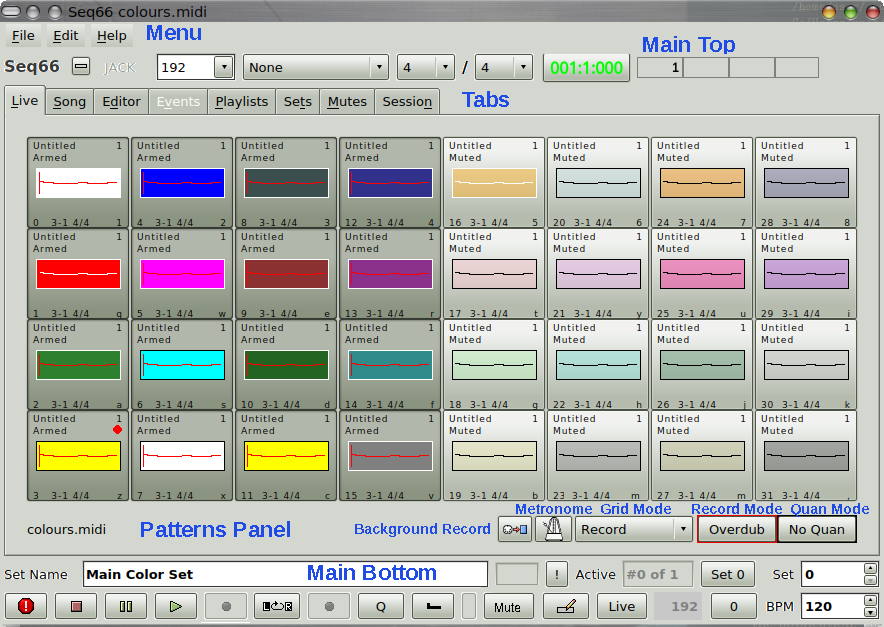
\includegraphics[scale=0.65]{main-window/main-window-annotated.png}
   \caption{Seq66 Main Screen, Annotated}
   \label{fig:main_screen_annotated}
\end{figure}

   The \textsl{Seq66} main window (i.e. the "Live Grid") appears as shown above.
   This figure has many differences from the \textsl{Seq24} main window,
   but the functionality is similar.
   \textsl{Seq66} allows resizing, and can
   be configured to start with its size scaled up or down.
   There is also a button near the top left that can
   hide the menu and the bottom panels, to allow reducing the
   size of the window event further.
   The features of the main window, including the "look" of the application,
   can be configured via the 'rc', 'usr', 'ctrl', 'drums', 'playlist', 'mutes',
   and 'palette' configuration files, via command-line options, via
   desktop themes, and via Qt ('qss') style-sheets.
   We break the discussion into sections for the following
   groups shown in the figure above:

   \begin{itemize}
      \item \textbf{Tabs}
      \item \textbf{Main Top}
      \item \textbf{Main Bottom}
      \item \textbf{Menu}
   \end{itemize}

\subsection{Tabs}
\label{subsec:introduction_main_tabs}

   The following tabs are present in \textsl{Seq66}:

   \begin{itemize}
      \item \textbf{Live}
      \item \textbf{Song}
      \item \textbf{Editor}
      \item \textbf{Events}
      \item \textbf{Playlists}
      \item \textbf{Sets}
      \item \textbf{Mutes}
      \item \textbf{Session}
   \end{itemize}

   We present brief descriptions here and links to sections with more detail.
   All tabs are discussed in more detail, each in its own section.

\subsubsection{Tabs / Live}
\label{subsubsec:introduction_main_tabs_live}

   The \textbf{Live} tab is foremost in the application.
   It provides a grid of \textsl{patterns}
   (also called \textsl{slots}, \textsl{loops}, \textsl{tracks}, or
   \textsl{sequences}) that display recorded MIDI data, status information, and
   provide popup-menus for each pattern.
   The buttons can
   be colored via a palette, and the status is easy to see
   from the coloring of activated buttons and a label that says "Armed"
   versus "Muted".
   The buttons can be toggled by a keystroke, shown in the lower
   right corner of the button.
   Another name for the \textbf{Live} tab is the \textbf{Patterns Panel};
   it can be replicated in multiple external windows.
   See \sectionref{sec:patterns_panel}.

\subsubsection{Tabs / Song}
\label{subsubsec:introduction_main_tabs_song}

   The \textbf{Song Editor} combines all patterns
   into a complete tune with controlled repetitions of each pattern.
   It provides a way to lay out \textsl{triggers} for each pattern
   that control playback without musician interaction.
   The editing capabilities of the song editor are extensive, including
   dragging triggers, addition transposition to triggers, and more.
   See \sectionref{sec:song_editor}.

\subsubsection{Tabs / Editor}
\label{subsubsec:introduction_main_tabs_editor}

   The \textbf{Pattern Editor} allows for the recording and editing of
   notes and other MDII events.
   It can be shown in the \textbf{Editor} tab or in an
   external window.  When opened in the tab, the pattern editor is compressed
   vertically by reducing the height of the "data" area and removing some
   buttons.  Otherwise, the pattern editor works the same in the tab and in
   external windows.
   See \sectionref{sec:pattern_editor}.

\subsubsection{Tabs / Events}
\label{subsubsec:introduction_main_tabs_events}

   The \textbf{Event Editor} provides a way to see the details of events
   and to do some modifying of them.  It's meant for light usage; there are
   some less-used events that it cannot edit.
   It is especially useful in trouble-shooting a song.
   See \sectionref{sec:event_editor}.

\subsubsection{Tabs / Playlist}
\label{subsubsec:introduction_main_tabs_playlist}

   The \textbf{Playlist Editor} is meant for the creation of
   play-lists.  One can create multiple playlists with multiple songs in each
   playlist.  The selection of playlists and songs can be done via keystrokes
   or MIDI control.
   Note that editing of the playlists can also be done by directly editing a
   \texttt{.playlist} file.  See \sectionref{sec:playlist}.

\subsubsection{Tabs / Sets}
\label{subsubsec:introduction_main_tabs_sets}

   The \textbf{Sets Editor} allows one to see, edit, and rearrange the sets
   that a tune contains.  Sets are also referred to as "banks".
   A useful feature of sets is that they can selected and cause a major change
   in the patterns that are playing.
   See \sectionref{sec:setmaster}.

\subsubsection{Tabs / Mutes}
\label{subsubsec:introduction_main_tabs_mutes}

   Mute-groups provide a way to turn on and turn off multiple patterns at once
   via a keystroke or a MIDI control; the \textbf{Mutes Editor} also provides a
   way to use buttons to control the mute-group.
   Mute-groups can be saved in the
   \texttt{.mutes} file or in the tune itself.
   See \sectionref{sec:mutes_master}.

\subsubsection{Tabs / Session}
\label{subsubsec:introduction_main_tabs_session}

   The \textbf{Session} tab displays some aspects of the running setup of
   \textsl{Seq66}.  It displays the name of the session manager, if any, client
   IDs, etc.  It also has a button reload the whole session after configuration
   changes are made.

   Here, a session log file can also be specified.
   If defined, then all messages written to the terminal when \textsl{Seq66}
   is run from a terminal shell are instead redirected to this file.
   The default log file is \texttt{seq66.log} specified to use
   the "home" directory.
   This file can be cleared using the button to the right of it; however,
   messages will continue to be logged to this file until
   \textsl{Seq66} is completely exited and then manually restarted.

   In addition, text data for patterns can be viewed and edited here.
   Select the desired pattern, enter the desired text, and click the
   \textbf{Save Info} button.
   The song is now modified and can be saved.

   Also see \sectionref{sec:sessions}.

\subsection{Main Top Controls}
\label{subsec:introduction_main_top_controls}

   Here, we first discuss the top and bottom \textbf{Main} controls, as
   shown in the following collapsed figure:

\begin{figure}[H]
   \centering 
%  \includegraphics[scale=0.75]{main-window/main-window-controls.png}
   \includegraphics[scale=0.75]{main-window/main-window-top.png}
   \caption{Main Window Top Controls}
   \label{fig:main_window_top_controls}
\end{figure}

   See the following section and
   \sectionref{subsec:introduction_main_bottom_controls}.
   The top panel of the Pattern window is simple, consisting of the
   name of the program and a few controls.
   The top main control items are, from left to right:

   \begin{itemize}
      \item \textbf{Seq66 Logo}
      \item \textbf{Show/Hide Button}
      \item \textbf{Engine Status}
      \item \textbf{PPQN Selection}
      \item \textbf{Buss Override for Play-set}
      \item \textbf{Global Beats Per Measure}
      \item \textbf{Global Beat Width}
      \item \textbf{BBT/HMS Time Display}
      \item \textbf{Beat Indicator Bar}
   \end{itemize}

   The status indicators that can appear to the right of the logo:

   \begin{itemize}
      \item \textbf{ALSA} appears if running using ALSA for MIDI.
      \item \textbf{JACK} appears if running using JACK for MIDI.
      \item \textbf{JACK Master} appears if running using JACK transport, as
         transport master.
         JACK transport can be used even if using ALSA for MIDI.
      \item \textbf{JACK Slave} appears if using JACK transport as
         transport slave.
      \item \textbf{Portmidi} appears if using the internal portmidi-derived
         MIDI engine.  This is currently always the case on \textsl{Windows}.
   \end{itemize}

\subsubsection{Show/Hide Button}
\label{subsubsec:introduction_show_hide_button}

   If present (it is a build option),
   this button at the left of the top bar
   allows the main menu and the bottom two
   rows of controls to be hidden.
   This measure can save a lot of space (e.g. in a \textsl{Raspberry Pi}
   setup.
   If your window manager (e.g. \textsl{Fluxbox})
   allows hiding the window decorations, the smallest useful size of the
   main window can be about 450 x 320 pixels.
   A good 'ctrl' automation file (e.g. for the \textsl{LaunchPad})
   is necessary to control \textsl{Seq66} in this tiny setup;
   main menu hot-keys are not accessible with the main menu hidden.

\begin{figure}[H]
   \centering 
   \includegraphics[scale=1.0]{main-window/main-window-tiny.png}
   \caption{Main Window Tiny (shown full size)}
   \label{fig:main_window_tiny}
\end{figure}

   Most of the other tabs are not usable at this small size,
   as they are too "busy" with many editing elements, and
   \textsl{Seq66} does not shrink or expand them.

%  Might be enough for live play?
%  Perhaps we should add a 'usr' option for the "tiny" mode?
%  And hide the rest of the tabs?  Switch some buttons around?

\subsubsection{PPQN Selection}
\label{subsubsec:introduction_ppqn_selection}

   This drop-down allows one to change the pulses-per-quarter-note (PPQN) of the
   loaded tune, and this change can then be saved, if desired, with the file.
   As with \textsl{Seq24}, the default PPQN is 192.
   \texttt{32, 48, 96, 120, 192, 240, 384, 768, 960, 1920, 2400, 3840,
   7680, 9600, and 19200}.
   The PPQN cannot be changed to to values not in this list, though.
%  Values, even weird ones, can be entered by typing them.
%  However, some values, such as 120, are not
%  displayed properly in the grids.
%  (Modify the file to use a supported value, if possible.)
   If a MIDI file is loaded, this modifies that file, rescaling all the
   pattern events and pattern triggers.
   Also see \sectionref{paragraph:menu_edit_preferences_play_options}.

\subsubsection{Buss Override for Play-set}
\label{subsubsec:introduction_sets_buss_override}

   This drop-down allows for overriding the buss (port) number used by all of
   the patterns in the current play-set.
   Unlike the \texttt{buss-override} setting in the 'usr' file
   (see \sectionref{subsubsec:usr_file_user_midi_settings}),
   this action causes a modification of the file (and a prompt to save at
   exit).

   \index{play-set}
   The \textsl{play-set} is the current set of patterns to be played.
   Normally, this set holds only the active patterns in the current
   play-screen.
   However, it can also be configured to include patterns from other sets.
   (See \sectionref{subsec:configuration_rc}.)

   The list of
   output busses is either the existing MIDI ports on the system, or,
   if port-mapping (see \sectionref{sec:port_mapping}) is active, the list
   of mapped output ports.
   Port-mapping is a useful way to redirect the set to a different output
   device; it can be used to provide a full set of virtual devices that any of
   the user's sequences can depend on.

   \index{--bus option}
   Another way to specify busses is the
   \texttt{-{}-buss n} command-line option.
   It causes \textsl{every} pattern in \textsl{every} set in the MIDI
   file to be directed to that buss number, and when a new
   sequence/pattern is created.  This option is only
   for convenience in testing.  Save the file, and it will
   have that buss number as part of each track's data, which makes the song
   file less portable, so be careful with both options.

\subsubsection{Global Beats Per Measure}
\label{subsubsec:introduction_global_beats_per_measure}

   This drop-down changes the global beats/measure for the song.
   Along with the beat-width setting, this set of values allows
   for a large number of different time signatures, even crazy ones.
   \textsl{Warning}: It modifies every pattern in the song, but is not
   otherwise saved in the configuration.
   Values: \texttt{1 to 16, 32}

\subsubsection{Global Beat Width}
\label{subsubsec:introduction_global_beat_width}

   This drop-down changes the global beat width (time-signature denominator)
   for the song.
   Along with the beats-per-measure setting, this set of values allows
   for a large number of different time signatures.
   \textsl{Warning}: It modifies every pattern in the song, but is not
   otherwise saved in the configuration.
   Values: \texttt{1 to 16, 32}

\subsubsection{BBT or HMS Time Display}
\label{subsubsec:introduction_time_display}

   This push-button shows the current time during playback. 
   It can be shown in BBT (bars:beats:ticks) or HMS (hours:minutes:seconds),
   which can be switched by clicking this button.
   (The \textbf{BBT/HMS} at the bottom of the window has been removed.)

\subsubsection{Beat Indicator}
\label{subsubsec:introduction_beat_indicator}

   The beat indicator is inspired by the \textsl{Kepler34} implementation.
   It shows the first beat in color, and the rest of the beats in the theme
   color.
   It does not adapt to changes in the time-signature until
   playback is stopped.

\subsection{Patterns Panel (Live Grid)}
\label{subsec:introduction_main_live_grid}

   In the center of the main window is the \textsl{patterns panel}, also 
   known as the \textsl{live grid}, where patterns/loops/tracks are shown
   and where they can be controlled.
   A MIDI file can be dragged-and-dropped onto the live grid in order
   to open it.
   Also shown in the patterns panel are a
   background-record button, metronome button, a
   grid-mode dropdown to control how the grid is used,
   a button to choose how recording works (e.g. overdub versus merge), and
   a button to indicate how recording is quantized.
   The patterns panel is discussed in more detail in
   \sectionref{sec:patterns_panel}.

\subsection{Main Bottom Controls, First Row}
\label{subsec:introduction_main_bottom_controls}

   The bottom main control items take up two rows.
   Here is the first row and its contents:

\begin{figure}[H]
   \centering 
   \includegraphics[scale=0.75]{main-window/main-window-bottom-1.png}
   \caption{Main Window Bottom, First Row}
   \label{fig:main_window_bottom_1}
\end{figure}

   \begin{itemize}
      \item \textbf{Set Name}
      \item \textbf{MG} (Mute Group)
      \item \textbf{Underrun Indicator}
      \item \textbf{Active Set Indicator}
      \item \textbf{Set Reset ("!")}
      \item \textbf{Set 0 Selector}
      \item \textbf{Set Changer}
   \end{itemize}

\subsubsection{Set Name}
\label{subsubsec:introduction_mg}

   This text field shows the name of the current set, and also allows editing
   the set name.
   The existing sets can be seen in the \textbf{Sets} tab.

\subsubsection{MG (Mute Group)}
\label{subsubsec:introduction_mute_group}

   This text field shows the name of the current mute-group, if one is
   in force. The existing mute-groups, if any, can be seen in the
   \textbf{Mutes} tab, or in the active 'mutes' files specified in the
   'rc' main configuration file.

\subsubsection{Underrun Indicator}
\label{subsubsec:introduction_underrun_indicator}

   This text field is empty under normal circumstances, including during
   playback.  However, if one opens a pattern editor for a pattern with a lot
   of events, and turns on recording for that pattern, then this field might
   start flashing numbers, which indicate the
   current underrun value in microseconds.  This gives an indication that
   timing of playback might be off a bit, usually less than 10 milliseconds.
   This happens because the event-list is locked during redrawing,
   when recording, to avoid problems when new notes come in.

\subsubsection{Set Reset ("!")}
\label{subsubsec:introduction_set_reset}

   This small button with an exclamation point
   to the right of the set name is meant to clear
   out all playing sets, and make only the current set the playing set.
   This button is useful when in "all-sets" mode or when sets get added
   automatically via the "additive" mode, so that multiple sets are playing
   at once.
   See \sectionref{subsec:configuration_rc}.

\subsubsection{Set Master Button}
\label{subsubsec:introduction_set_master_button}

   The Set Master button has been removed.
   The external window it used to bring up has been replaced
   by the \textbf{Set Master} tab.

%  This button brings up an external window showing the
%  panel.  This panel is also available in a center tab.  It is a work in
%  progress, and doesn't have a whole lot of functionality yet.
%  It can currently show existing sets in one view, and allow
%  reordering the sets.

\subsubsection{Active Set Indicator}
\label{subsubsec:introduction_active_set_indicator}

   This read-only text field shows the set number of the currently active set.
   One can open a number of external \textsl{Live Frames} by
   \textsl{shift-left-clicking} on pattern slots.
   The currently active set is then the
   set that has the mouse focus.  This allows for working with multiple sets
   without a lot of mouse/keyboard navigation.
   Note that there is always at least one set in a \textsl{Seq66}
   tune.

\subsubsection{Set 0}
\label{subsubsec:introduction_set_zero}

   This button provides a fast way to get back to set 0, without clicking the
   mouse a bunch of times.
   It is useful when creating an external live grid
   (see \sectionref{fig:multiple_live_grids}),
   which currently also sets the main grid to the same set.
   Click on this button, and the external set and set 0 can be seen at the same
   time.

\subsubsection{Set Changer}
\label{subsubsec:introduction_set_changer}

   This spin-box allows showing a different set in the main windows.
   This set can be modified by adding new patterns, changing its name, or
   importing other MIDI files into the current set.

\subsection{Main Bottom Controls, Second Row}
\label{subsec:introduction_main_bottom_controls_2}

   Here is the second row and contents:

\begin{figure}[H]
   \centering 
   \includegraphics[scale=0.75]{main-window/main-window-bottom-2.png}
   \caption{Main Window Bottom, Second Row}
   \label{fig:main_window_bottom_2}
\end{figure}

   \begin{itemize}
      \item \textbf{Panic}
      \item \textbf{Stop}
      \item \textbf{Pause}
      \item \textbf{Play}
      \item \textbf{Record Button}
      \item \textbf{L/R Loop}
      \item \textbf{Live Song Record}
      \item \textbf{Keep Queue}
      \item \textbf{Mute Group Learn}
      \item \textbf{Developer Test}
      \item \textbf{Mute} (Toggle Mute Status)
      \item \textbf{Song Editor}
      \item \textbf{Live/Song}
      \item \textbf{PPQN Indicator}
      \item \textbf{Tap BPM}
      \item \textbf{Beats Per Minute Control}
   \end{itemize}

   Many of these controls have keystrokes and MIDI-control slots that can be
   set up in the 'ctrl' file.

   Note that \textbf{BBT/HMS Toggle Button} has been removed
   (version 0.99.9).
   One can now click on the \textbf{BBT/HMS Time Display} to
   change the format.

\subsubsection{Panic}
\label{subsubsec:introduction_panic_button}

   This button causes playback to stop, all patterns to mute, and flushes the
   MIDI buss.
   There is a keystroke control and a MIDI control
   for this automation operation, plus
   a MIDI-announcement (output) configuration item for it.

\subsubsection{Stop}
\label{subsubsec:introduction_stop_button}

   This button stops playback and rewinds to the beginning of the song.
   By default, the \texttt{Esc} key operates this function,
   and there is both a MIDI-control slot and a MIDI-announcement slot
   available for it.

\subsubsection{Pause}
\label{subsubsec:introduction_pause_button}

   This button stops playback, but does not rewind to the beginning of the
   song.  It also resumes playback at the same point as the pause.  By default,
   the \texttt{Period} key operates this function, and there is a MIDI-control
   slot and a MIDI-announcement slot available for it.  This key is also
   hardwired to pause and start playback in the pattern editor and the song
   editor.

\subsubsection{Play}
\label{subsubsec:introduction_play_button}

   This button starts playback, either at the beginning or at the pause point.
   Also called the "start button".
   By default, the \texttt{Space} key operates this function,
   and there is both a MIDI-control slot and a MIDI-announcement slot
   available for it.
   This key is also hardwired to toggle playback in the pattern editor and the
   song editor.

\subsubsection{Record Button}
\label{subsubsec:introduction_record_button}

   This button turns on recording for the various kinds of recording
   described in \sectionref{sec:recording}.
   Its color indicates the record-by feature in force:

   \begin{itemize}
      \item \textbf{Grey}.
         No pattern is selected, so this button is non-functional.
      \item \textbf{Red}.
         This color indicates the normal recording mode, which toggles only a
         single pattern for recording.
         This button is enabled and colored red only if a pattern is the last
         one selected in the grid.
      \item \textbf{Yellow}.
         This color indicates the record-by-channel recording mode,
         which toggles, for recording, all patterns that have an
         output channel set.
         Incoming events that have a channel nybble are routed to that
         pattern.
      \item \textbf{Green}.
         This color indicates the record-by-buss recording mode,
         which toggles, for recording, all patterns that have an
         input bus set. This button is green only if there is at least
         one such pattern.
         A pattern can be assigned an input buss via its right-click
         menu, but only if
         \textbf{Edit / Preferences / MIDI Input / Record into patterns by bus}
         is enabled.
   \end{itemize}

   These modes are selected in the 'rc' file as described in
   \sectionref{subsubsec:configuration_rc_midi_cmt}.
   They are mutually exclusive.

\subsubsection{L/R Loop}
\label{subsubsec:introduction_loop_button}

   This button has been added to the main window.
   It also appears in the "external" version of the song editor.
   This reflects that the \textbf{L/R} loop markers in the song editor can now
   be used in the pattern editor as well.  This new feature makes it easier to
   focus in on a pattern and tinker repeatedly with the same small section.
   In addition, looping can now be done in both the Live and Song modes of
   playback.

   \index{loop mode}
   Activates loop mode. When play is activated, plays the song and loop
   between the
   \index{L marker}
   \index{R marker}
   \textbf{L marker} and the \textbf{R marker}.
   It is a state button, and its appearance indicates when it is
   depressed, and thus active.
   \textsl{If this button is deactivated during playback, then playback
   continues past the \textbf{R marker}.}
   Note that these markers can be placed using left
   and right mouse clicks, respectively, in the time/measures ruler.
   Furthermore, the \textbf{L/R} markers can also be set in a pattern editor,
   where they can be used to focus in on a small section of notes.
   Lastly, this looping mechanism is also available in Live mode as well.

\subsubsection{Live Song Record}
\label{subsubsec:introduction_live_record_button}

   This button causes a live playing session to be recorded to Song mode.
   That is, triggers are added to the song automatically as the musician mutes
   and unmutes patterns, and the triggers can then be
   seen as layouts in the \textsl{Song} editor.
%  FIXME:
%  By default, the \texttt{P} key operates this function.

   Using the \texttt{Ctrl} modifier while clicking this button
   turns off the recording-snap feature.
   This change can also be done in the song editor.
   Using the \texttt{Shift} modifier while clicking this button
   causes recording immediately after starting playback.
   This feature is useful in avoid delay at start up.

\subsubsection{Keep Queue}
\label{subsubsec:introduction_keep_queue_button}

   Puts the application into a "sticky" queue mode.
   In this mode, pressing a pattern key does not do a mute/unmute function, but
   instead turns on queuing for the selected pattern.
   By default, the \texttt{Backslash} key operates this function,
   and there is a MIDI-control slot available for it.

\subsubsection{Mute Group Learn}
\label{subsubsec:introduction_mute_group_learn_button}

   \index{L button}
   Also called the "L" button.
   Sets up to learn the current set of active patterns ("mute group") into a
   mute-group.
   The default keystroke to control this button is lower-case "L".
   When in group-learn mode, the \texttt{Shift} key cannot be hit, so the
   group-learn mode automatically converts the keys to their shifted versions.
   This feature known as \textsl{shift-lock} or \textsl{auto-shift}.
   This feature is not used if a non-QWERTY keyboard layout is
   specified in the 'ctrl' file.

   After pressing the "L" button, the user can then press a keystroke, which is
   automatically shifted, and the pattern set is saved, and can be recalled by
   pressing that button, shifted, later.
   It can be saved in a 'mutes' file, as part of
   the MIDI tune, or in both places.

   \textsl{Example}:
   We have 5 patterns armed in the current set. Press the "L" button,
   and then press the "s" key.  These pattern statuses are saved and can be
   recalled later by the "S" ("s"-shifted) key.

   By default, the \texttt{el} (lower-case "L") key also sets this function,
   and there is a MIDI-control slot available for it, as well as a
   MIDI-announcement slot.
   In addition to that, one can also press
   the \texttt{Ctrl-L} key.
   The "el" with it!

   Remember that groups work with the playing ("in-view") screen-set.
   One must change the screenset and give it the command to make it the
   playing one.
   \index{keys!Home}
   By default, the \texttt{Home} key is configured for this purpose.

   There is also a setting in the 'mutes' file called
   \texttt{mute-group-selected}.  If this value is set to a value from 0 to 31,
   then that mute group will be automatically applied when
   \textsl{Seq66} starts up.
   This is useful with the loading of the most-recent MIDI file (which is also
   a feature of \textsl{Seq66}.
   Also see the section about the "mute master" tab,
   \sectionref{sec:mutes_master}.

\subsubsection{Developer Test}
\label{subsubsec:introduction_developer_test_button}

   This button is always disabled.  Functionality is added temporarily when
   testing new features. Ignore this button.

\subsubsection{Toggle Mute Status}
\label{subsubsec:introduction_toggle_mute_status_button}

   The \textbf{Mute}  button toggles the mute/armed status of all of the
   patterns in the current set.
   Works the same as the
   \textbf{Edit / Toggle All Tracks} menu or the hard-wired
   \texttt{Ctrl-T} key.
   There is also an automation control entry for it, associated by
   default with \texttt{F8}.
   As of version 0.99.16, it is no longer disabled in Song Mode.

\subsubsection{Song Editor}
\label{subsubsec:introduction_song_editor_button}

   This button (with a "pencil" icon)
   brings up an external window for editing the Song/Performance
   information.  If already up, it closes it.
   Works the same as the
   \textbf{Edit / Song Editor} menu or the hard-wired \texttt{Ctrl-E} key.

\subsubsection{Live/Song Mode}
\label{subsubsec:introduction_livesong_mode_button}

   This button toggles between the \textsl{Live} and \textsl{Song} performance
   mode. In the Live mode, the musician controls are muting/unmuting of each
   pattern.  In the Song mode, the triggers layed out in the
   \textbf{Song Editor} control the playback.
   By default, the \texttt{F10} key operates this function,
   There is also a MIDI automation control for this button.

\begin{comment}
   \itempar{Toggle Tracks}{pattern!toggle tracks}
   \index{pattern!toggle tracks}
   This button changes the status of all of the
   \textsl{playing} tracks, reversing the
   mute status of each pattern that is playing.
   The next click will then unmute only those tracks.
   Because it can be confusing, this button is disabled
   in Song mode.

   The \texttt{Ctrl-M}, \texttt{Ctrl-U}, and \texttt{Ctrl-T} keys,
   as shown in the \textbf{Edit} menu, mute, unmute, and toggle
   all patterns.

\end{comment}

\subsubsection{PPQN Indicator}
\label{subsubsec:introduction_ppqn_indicator}

   This read-only field displays the current PPQN for the current tune.

   \configref{usr}{user-midi-settings}{midi\_ppqn}

\subsubsection{BBT/HMS Toggle (removed)}
\label{subsubsec:introduction_time_format_toggle_button}

   The time display has been converted to a button, and click it will
   switch the format. So the BBT/HMS Toggle button
   \textsl{has been removed}.
   See the top bar for the time display/button.

%  Toggles the format of the current time displayed during playback. 
%  It can be shown in B:B:T (bars:beats:ticks) or H:M:S (hours:minutes:seconds).

\subsubsection{Tap BPM Button}
\label{subsubsec:introduction_tap_bpm_button}

   Tap this button with a regular beat to determine the beats-per-minute of the
   tapping.  With each tap, the counter on the button increments and the BPM is
   recalculated.  Stop tapping for a few seconds to reset the counter.
   By default, the \texttt{F9} key operates this function, but it
   There is also a MIDI-control slot for this function, and
   \texttt{F9} is the default key for this function.

\subsubsection{Beats Per Minute Control}
\label{subsubsec:introduction_bpm_control}

   This control can be text-edited or spun to change the beats/minute value
   used in playing back the current song.  This value is also saved to the
   file.

%-------------------------------------------------------------------------------
% vim: ts=3 sw=3 et ft=tex
%-------------------------------------------------------------------------------


% Menu

%-------------------------------------------------------------------------------
% menu
%-------------------------------------------------------------------------------
%
% \file        menu.tex
% \library     Documents
% \author      Chris Ahlstrom
% \date        2015-08-31
% \update      2025-05-30
% \version     $Revision$
% \license     $XPC_GPL_LICENSE$
%
%     Provides the Menu section of seq66-user-manual.tex.
%
%-------------------------------------------------------------------------------

\section{Menu}
\label{sec:menu}

   The \textsl{Seq66} menu structure is more complex than
   that of \textsl{Seq24}.  In particular, the \textsl{File} menu has two
   variants:  a normal file menu, and a file menu when \textsl{Seq66} is
   running under the \textsl{New/Non Session Manager}.
   (See \sectionref{subsec:sessions_nsm}.)

\subsection{Menu / File}
\label{subsec:menu_file}

   The \textbf{File} menu is used to save and load files in
   Standard MIDI Format 0 or 1, \textsl{Cakewalk} "WRK",
   and \textsl{Seq66} MIDI files.
   It also supports a list of recent files, and
   sub-menus for import and export functions,
   which have expanded quite a bit.
   The \textsl{Seq66} \textbf{File} menu contains the sub-items shown below.
   The next few sub-sections discuss
   the sub-items in the \textbf{File} menu.
   Please note that these entries are different
   if \textsl{Seq66} is started under the control of the
   \textsl{New/Non Session Manager}.  
   See \sectionref{subsubsec:sessions_file_menu}.
   However, the import and export menus remain the same, although there are
   slight differences in how they work.

\begin{figure}[H]
   \centering 
   \includegraphics[scale=0.75]{main-menu/file/file-import-export-menus.png}
   \caption{Seq66 File Menu Plus Import/Export, Composite View}
   \label{fig:menu_file_items}
\end{figure}

   \begin{enumber}
      \item \textbf{New}
      \item \textbf{Open}
      \item \textbf{Open Playlist}
      \item \textbf{Recent MIDI files}
      \item \textbf{Save}
      \item \textbf{Save As}
      \item \textbf{Import}
      \begin{enumber}
         \item \textbf{Project Configuration...}
         \item \textbf{MIDI to Current Set...}
         \item \textbf{Playlist...}
         \index{restart!automatic}
         Once the playlist is imported,
         \textsl{Seq66} is automatically \textsl{\textbf{restarted}}
         in order to load the playlist.
         Be careful!
      \end{enumber}
      \item \textbf{Export}
      \begin{enumber}
         \item \textbf{Project Configuration...}
         \item \textbf{MIDI Only...}
         \item \textbf{Song...}
         \item \textbf{SMF 0...}
      \end{enumber}
      \item \textbf{Quit} (\textbf{Exit} in \textsl{Windows})
   \end{enumber}

   For information on the \textbf{File} menu when \textsl{Seq66} is
   running under the \textsl{Non Session Manager}, see
   \sectionref{subsubsec:sessions_file_menu}.

\subsubsection{Menu / File / New}
\label{subsec:menu_file_new}

   The \textbf{New} menu entry clears the current song.
   (A play-list or mute-groups setup, if loaded, are not affected.)
   If unsaved changes are pending, the user is prompted to save the changes.
   Prompting for changes is more comprehensive than \textsl{Seq24}.
   However, when in doubt, save!
   Keep backups of your tunes and configuration files!

\subsubsection{Menu / File / Open}
\label{subsubsec:menu_file_open}

   The \textbf{Open} menu entry opens a song (MIDI file or \textsl{Cakewalk}
   WRK file), replacing the current song (after a prompt if the song was
   modified).
   It opens up a standard file dialog:

\begin{figure}[H]
   \centering 
   \includegraphics[scale=0.65]{main-menu/file/light-menu-file-open.png}
   \caption{File / Open}
   \label{fig:menu_file_open}
\end{figure}

   This dialog lets one type a file-name, highlighting the first file
   that matches the characters typed.
   \textsl{Seq66} can open \textsl{Seq66}, MIDI SMF 0, and SMF 1 files, and
   \textsl{Cakewalk} WRK files.
   If the file is an SMF 0 file, where all channels appear on one track, the
   track can be split so that each channel (0 to 15)
   is stored in the corresponding
   pattern, and pattern 16 contains the original track.
   This feature is enabled via
   \textbf{Edit / Preferences / Pattern / Automatic conversion of SMF 0 to SMF
   1} or the 'usr' setting \texttt{convert-to-smf-1 = true}.

   Note that a MIDI file can be drag-and-dropped from a file manager onto
   the grid to open a file.

\subsubsection{Menu / File / Open Playlist}
\label{subsubsec:menu_file_open_playlist}

   The \textbf{Open Playlist...} menu entry opens a \textsl{Seq66}
   play-list file.

\begin{figure}[H]
   \centering 
   \includegraphics[scale=0.65]{main-menu/file/dark-menu-file-open-playlist.png}
   \caption{File / Open Playlist}
   \label{fig:menu_file_open_playlist}
\end{figure}

   The playlist file contains a list of "playlist sections",
   each listing a number of MIDI songs.
   These playlists and songs can be
   selected by the arrow keys or by MIDI control,
   and are displayed and editiable in the \textsl{Playlist} tab
   in the main window.
   See \sectionref{sec:playlist}.

\subsubsection{Menu / File / Recent MIDI files}
\label{subsubsec:menu_file_recent}

   This menu entry provides a list of the last few MIDI files created or opened;
   play-list selections are \textsl{not} included in this list.

\begin{figure}[H]
   \centering 
   \includegraphics[scale=0.65]{main-menu/file/menu-recent-files.png}
   \caption{Seq66 Menu File Recent Files}
   \label{fig:menu_file_recent_files}
\end{figure}

   Here is the long form when the 'rc' file's
   \texttt{[recent-files] full-paths} value is set to true:

\begin{figure}[H]
   \centering 
   \includegraphics[scale=0.65]{main-menu/file/menu-recent-files-long.png}
   \caption{Seq66 Menu File Recent Files, Full Paths}
   \label{fig:menu_file_recent_files_full_paths}
\end{figure}

   This list is saved in the \texttt{[recent-files]} section of the
   'rc' configuration file.
   In the 'rc' file, the full path to the file-name is stored.
   This path is in "UNIX" format, using the forward slash (solidus),
   as the path separator, even in \textsl{Windows}.
   The \texttt{full-paths} option can be set to show the full path in the
   recent-files drop-down menu.
   Only unique entries are included in the recent-files list.
   The limit is 12 recent-file entries.
   This is a feature from \textsl{Kepler34} \cite{kepler34}.
   One can also set \textsl{Seq66} to load the most-recent file at startup.
   Here is an example from an 'rc' file:

\begin{verbatim}
   [recent-files]
   full-paths = false
   load-most-recent = true
   count = 3
   /home/user/git/seq66/data/b4uacuse-gm-patchless.midi
   /home/user/git/seq66/data/midi/colours.midi
   /home/user/git/Julian-data/TestBeeps.midi
\end{verbatim}

\subsubsection{Menu / File / Save and Save As}
\label{subsubsec:menu_file_open_save_as}

   The \textbf{Save} menu entry saves the song under its current file-name.
   If there is no current file-name, it opens up a standard file
   dialog to name and save the file.
   The \textbf{Save As} menu entry saves a song under a different name.
   It opens up the following standard file dialog, very similar to the 
   \textbf{File Open} dialog, with an additional \textbf{Name} text-edit field.
   The exact look of the dialog depends on system Qt settings or the current
   Qt theme.

\begin{figure}[H]
   \centering 
   \includegraphics[scale=0.65]{main-menu/file/dark-menu-file-save-as.png}
   \caption{File / Save As}
   \label{fig:menu_file_save_as}
\end{figure}

   To save a new file or save the current file to a new name,
   enter the name in the name field, without an extension.
   \textsl{Seq66} will append a \texttt{.midi} extension to the filename.
   The file will be saved in a format that the Linux \textsl{file} command
   will tag as something like:

   \begin{verbatim}
      colours.midi: Standard MIDI data (format 1) using 16 tracks at 1/192
   \end{verbatim}

   It looks like a simple MIDI file, and yet, if one re-opens it in
   \textsl{Seq66}, one sees that the mute-groups, labeling, pattern
   information, and song layout have been preserved in this file.
   This information is saved in a way that MIDI-compliant software
   should be able to use or ignore without failure.
   After the last track in the file, a number of
   \index{SeqSpec}
   sequencer-specific (SeqSpec) items are saved, to preserve
   the extra information that \textsl{Seq66} adds to the song.
   There is no way to save a \textsl{Cakewalk} "WRK" file.
   \textsl{Seq66} can only read them, and then save them as
   \textsl{Seq66} files.

   \index{Meta events}
   Meta events are now handled by \textsl{Seq66}.
   Meta events \textbf{Set Tempo}
   and \textbf{Time Signature}
   are now fully supported.
   Other meta events,
   such as \textbf{Meta MIDI Channel}
   and \textbf{Meta MIDI Port}
   are now read as events, and are saved back when the file is saved.
   They cannot be edited in \textsl{Seq66}, but they are not lost.
   (Channel and port meta events are
   considered \textsl{obsolete} in the MIDI standard.)
   Various meta text events, such as \textbf{Lyric},
   can be edited and saved.

\subsubsection{Menu / File / Import / Project Configuration}
\label{subsubsec:menu_file_import_project_configuration}

   This command is useful to grab an existing project configuration
   (i.e. the set of \texttt{qseq66.*} files) and copy it
   to the current "home" configuration directory.
   This command is most useful in importing a project into a new
   NSM session.
   Previously, the "home" project would be imported automatically
   into a new NSM session, but this was deemed confusing by some users, and
   properly so!

   This command brings up a file dialog box. Navigate to the desired
   source directory and then select the desired 'rc' file.
   Any configuration files in the current "home" directory are removed
   and replaced with all files and subdirectories from the selected
   directory.
   If NSM is not running, \textsl{Seq66} restarts and loads the
   imported configuration.
   Be aware!
   Otherwise, a prompt to restart using the NSM client is shown.
   For more information, see
   \sectionref{subsubsec:midi_export_file_import_project}.

\subsubsection{Menu / File / Import / MIDI to Current Set}
\label{subsubsec:menu_file_import}

   The \textbf{Import} menu entry imports an SMF 0
   or SMF 1 MIDI file as one or more patterns, one pattern per track,
   into the specified screen-set.
   This functionality is explained in detail in
   \sectionref{subsubsec:midi_export_file_import}.

\subsubsection{Menu / File / Import / Playlist}
\label{subsubsec:menu_file_import_playlisMIDI to Current Sett}

   A user can create a playlist that accesses MIDI files anywhere in the file
   system.
   However, in a session manager, it is preferable to have the configuration
   self-contained.
   Even without a session manager, it can be useful to copy a playlist to a
   subdirectory in order to separate it and its MIDI files from other
   playlists.
   Once a project has been imported or saved, then a playlist can also be
   imported, along with all of the MIDI files it references.

   This command brings up a file dialog box. Navigate to the desired
   source directory and then select the desired 'playlist' file.
   This menu entry copies the playlist file and its associated
   MIDI files; see
   \sectionref{subsubsec:midi_export_file_import_playlist}.

\subsubsection{Menu / File / Export / Project Configuration}
\label{subsubsec:menu_file_export_project}

   This menu entry lets the user select a destination directory.
   Then the project files from the current "home" directory are copied
   to that destination directory. Useful for backup or for making
   an experimental configuration official.
   See \sectionref{subsubsec:midi_export_configuration_export}.

\subsubsection{Menu / File / Export / Song}
\label{subsubsec:menu_file_export_song_as_midi}

   Thanks to the \textsl{Seq32} project, the ability to export songs to MIDI
   format has been added.  In this export, a complete song performance is
   recoded so that other MIDI sequencers can play the performance properly.
   This functionality is explained in detail in
   \sectionref{subsubsec:midi_export_song_export}.

\subsubsection{Menu / File / Export / MIDI Only}
\label{subsubsec:menu_file_export_midi_only}

   Sometimes it might be useful to export only the non-vendor-specific
   (non-SeqSpec) data from a \textsl{Seq66} song, in order to reduce the
   size of the file or to accomodate non-compliant sequencers.
   This functionality is explained in detail in
   \sectionref{subsubsec:midi_export_file_export_midi_only}.

\subsubsection{Menu / File / Export / SMF 0}
\label{subsubsec:menu_file_export_smf_0}

   This feature allows all tracks in the song to
   be consolidated and exported in MIDI's SMF 0 format.
   It follows rules similar to song export.
   See \sectionref{subsubsec:midi_export_file_export_smf_0}.

\subsection{Menu / Edit}
\label{subsec:menu_edit}

   The \textbf{Edit} menu has undergone some expansion in \textsl{Seq66}.

   \begin{enumber}
      \item \textbf{Preferences...}
      \item \textbf{Song Editor}
      \item \textbf{Apply Song Transpose}
      \item \textbf{Clear Mute Groups}
      \item \textbf{Reload Mute Groups}
      \item \textbf{Mute All Tracks}
      \item \textbf{Unute All Tracks}
      \item \textbf{Toggle All Tracks}
      \item \textbf{Copy Current Set}
      \item \textbf{Paste To Current Set}
   \end{enumber}

   \setcounter{ItemCounter}{0}      % Reset the ItemCounter for this list.

   \itempar{Preferences}{edit!preferences}
   This entry brings up a \textbf{Preferences} menu entry,
   to allow viewing and tweaking MIDI I/O ports, displays options, JACK
   options, and more.
   It can also be brought up by \texttt{Ctrl-P}.
   It has a lot of configuration items, and is
   discussed in \sectionref{sec:edit_preferences}.

   \itempar{Song Editor}{edit!song editor}
   \index{performance editor}
   \index{song editor}
   This item toggles the presence of the main song/performance editor.
   Note that the song editor is also available in the
   \textbf{Song} tab in the main window.
   The song/performance editor allows specifying exact numbers of loop replays;
   this provides a canned rendition of all the patterns in theMIDI tune.

   \itempar{Apply Song Transpose}{edit!song transpose}
   \index{song transpose}
   Selecting this item applies the global song transposition value to
   all sequences / patterns marked as transposable.
   This actively changes the note / pitch value of all note and aftertouch
   events in every pattern.
   The change can range from -12 semitones to 12 semitones.
   For the setting of the global song transpose value, see
   \sectionref{sec:song_editor}.
   Normally, drum tracks are \textsl{not} transposable.
   This can be set by clicking the "transposable" button in the
   pattern editor.
%  Note that transpose can be enabled in the
%  in the sequence editor
%  (see \sectionref{sec:pattern_editor}).

   \itempar{Clear Mute Groups}{edit!clear mute groups}
   \index{mute groups}
   A feature of \textsl{Seq66} is that the mute groups
   can be saved in both the 'rc' file \textsl{and} in the "MIDI" file.
   This menu entry clears them. If this resulted in any mute-group sequences
   status being set to false, then the user is prompted to save the MIDI
   file, so that it will no longer have any
   mute-group information.  And then, if the
   application exits, the cleared mute-group information is also saved to
   the 'rc' file.

   \itempar{Reload Mute Groups}{edit!load mute groups}
   \index{rc!mute groups}
   This menu entry reloads the mute-groups from the 'rc' file.
   So, if one loads a MIDI file that has its own mute groups that one does not
   like, this command will restore one's favorite mute-grouping from the 'rc'
   file.

   \itempar{Mute All Tracks}{edit!mute all tracks}
   \index{mute all}
   This menu entry, useful mostly in \textbf{Live} mode,
   immediately mutes \textsl{all} patterns in the entire song.
   The hard-wired menu short-cut for this action is \texttt{Ctrl-M}.

   \itempar{Unmute All Tracks}{edit!unmute all tracks}
   \index{unmute all}
   This menu entry, useful mostly in \textbf{Live} mode,
   immediately unmutes \textsl{all} patterns in the entire song.
   The hard-wired menu short-cut for this action is \texttt{Ctrl-U}.

   \itempar{Toggle All Tracks}{edit!toggle all}
   \index{toggle all}
   This option toggles the mute/armed status of \textbf{all} tracks.
   It is useful mostly \textbf{Live} mode, which overrides \textbf{Song}
   mode even if the Song Editor is focused.
   The hard-wired menu short-cut for this action is \texttt{Ctrl-T}.
   The default keystroke in the 'ctrl' file is \texttt{F8}.

   \itempar{Copy Current Set}{edit!copy set}
   \index{copy set}
   This item marks the current set (i.e. the play-set)
   for the copying of all its patterns to another set.
   After clicking this menu entry, one can move to another set to paste it,
   using the following menu entry.

   \itempar{Paste To Current Set}{edit!paste set}
   \index{paste set}
   Once a set has been copied into the internal set clipboard,
   then this menu item is enabled.
   Move to the desired set (whether empty or note), and then
   click this menu item.
   All of the patterns in the original set are pasted into the current set,
   \textsl{overwriting all patterns} already in the set.
   Also note that the set clipboard can be pasted after a
   \textbf{File / New} or \textbf{File / Open},
   to copy it into another file.

\subsection{Menu / Help}
\label{subsec:menu_help}

   The usual \textbf{Help} dialog is provided.
   As of version 0.98.8, it has been beefed up with a way to access a
   tutorial and the user manual.

   These new help items are a work in progress, so please apprise
   us of any issues; include information on the operating system and,
   if \textsl{Linux}, the desktop/window manager in use.

\subsubsection{Menu / Help / About...}
\label{subsubsec:menu_help_about}

   \index{Help!about}
   This menu entry shows the "About" dialog.
   That dialog provides access to some credits for the program as well.
   authors and the project documentors, and active link to them.
   It also shows Git version-control information as well.

\subsubsection{Menu / Help / Build Info...}
\label{subsubsec:menu_help_build_info}

   \index{Help!build info}
   This menu entry shows the "Build Info" dialog.  This list of
   build options enabled in the current application is the same list
   that it generated via this command line:

   \begin{verbatim}
      $ seq66 --version
   \end{verbatim}

\subsubsection{Menu / Help / Song Summary File...}
\label{subsubsec:menu_help_song_summary_file}

   \index{Help!song summary}
   This menu entry allows one to write a summary of the song data into a text
   file. It brings up a file dialog which defaults to the name of the
   currently-loaded MIDI file, with the extenstion \texttt{.text} and
   the directory from where the MIDI file was loaded.
   It shows the filename, the information about the sets and tracks,
   MIDI format (0 or 1), and the PPQN.

   It also shows each sequence: name, channel (128 mean there is no output
   channel), the time signature, buss number (and any mapping), the length in
   pulses, the event and trigger count, transposability, key and scale, and
   color number (if any).
   For each trigger in the pattern, its start, stop, offset, and transposition
   values are shown.
   This file can be helpful for trouble-shooting or solving puzzling effects in
   the tune.

\subsubsection{Menu / Help / App Keys}
\label{subsubsec:menu_help_app_keys}

   \index{Help!app keys}
   This entry brings up a dialog that shows brief descriptions of the
   non-automation keys available in various contexts.
   These keys are almost exclusively hardwired and currently cannot be
   changed via a configuration file.  By pressing a button, the desired
   keystrokes can be quickly viewed. Note that the descriptions come from small
   HTML files that are part of the installation.

\subsubsection{Menu / Help / Tutorial}
\label{subsubsec:menu_help_tutorial}

   \index{Help!tutorial}
   This entry brings up a short tutorial of \textsl{Seq66} in the default
   browser. This tutorial is meant only to jump-start a new user of
   \textsl{Seq66}, and is a work in progress.
   It does not cover nearly as much as the user manual, so check that out in
   the next section.

   Normally, the tutorial will open a web page.  If it does not, one might need
   to set up a default browser.  On Linux, make sure that there is a "desktop"
   file for the browser, as in
   \texttt{/usr/share/applications/firefox.desktop}.
   If so, then run the following command, and then test it:

   \begin{verbatim}
      $ xdg-settings set default-web-browser firefox.desktop
      $ xdg-open https://ahlstromcj.github.io/docs/seq66/tutorial/index.html 
   \end{verbatim}

   On Windows, this procedure is still \textsl{to be determined}.

   In both systems, one can override the default applications by opening
   the specified 'usr' file (usually \texttt{qseq66.usr} or
   \texttt{qpseq66.usr} and specifying the full path to the desired
   applications (Linux paths shown here):

   \begin{verbatim}
      [user-options]
      log = "/home/user/.config/seq66/seq66.log"
      pdf-viewer = "/usr/bin/zathura"
      browser = "/usr/bin/google-chrome"
   \end{verbatim}

   Also see \sectionref{subsubsec:usr_file_user_options}.

\subsubsection{Menu / Help / User Manual}
\label{subsubsec:menu_help_user_manual}

   \index{Help!user manual}
   This menu entry first tries to locate the user manual on the internet and
   open it in the default browser. If not found, or the network is down,
   then this entry brings up the full \textsl{Seq66} user manual in the default
   PDF viewer.  It currently looks in the possible installation areas and in
   the \textsl{Seq66} source tree to find the PDF.

   On Linux, one can follow the setup procedure in the previous section and
   test it via the following command, which will show the manual in the default
   browser.:

   \begin{verbatim}
      $ xdg-open https://ahlstromcj.github.io/docs/seq66/seq66-user-manual.pdf
   \end{verbatim}

%-------------------------------------------------------------------------------
% vim: ts=3 sw=3 et ft=tex
%-------------------------------------------------------------------------------


% Patterns Panel

%-------------------------------------------------------------------------------
% patterns_panel
%-------------------------------------------------------------------------------
%
% \file        patterns_panel.tex
% \library     Documents
% \author      Chris Ahlstrom
% \date        2015-08-31
% \update      2025-05-15
% \version     $Revision$
% \license     $XPC_GPL_LICENSE$
%
%     Provides the concepts.
%
%-------------------------------------------------------------------------------

\section{Patterns Panel}
\label{sec:patterns_panel}

   The main window of \textsl{Seq66} is
   where one creates a set of patterns (a "screen-set"),
   manages the configuration, controls the playback rate, adds tempo events,
   and opens the pattern, song, event, mute-groups, or playlist editors.

   \index{Patterns Panel}
   \index{Live Grid}
   The \textbf{Patterns Panel}, also called the \textbf{Live Grid},
   is the center of the
   \index{main window}
   \textbf{main window} of \textsl{Seq66}.
   It is also referred to as the "Live Grid", where each pattern is
   presented in a "slot".
   See \figureref{fig:main_screen_annotated} and
   \sectionref{sec:live_grid}.

   \index{drag and drop}
   In addition, an external MIDI file can be dragged onto this grid,
   and dropped, to easily open a MIDI file:

\begin{figure}[H]
   \centering 
   \includegraphics[scale=0.75]{main-window/live-grid-drag-n-drop.png}
   \caption{Patterns Panel Drag-and-Drop}
   \label{fig:patterns_panel_drag_n_drop}
\end{figure}

%  This drag-and-drop can be done even with "external" pattern editors.
   If a modified file is loaded, the user
   will be prompted to save, discard, or cancel.

   \textsl{Seq66} works with "patterns" (also known as "loops", "tracks", or
   "sequences") that are repeated throughout a song.
   One composes and edits small patterns in a grid,
   and combines them to create a full song.
   This is a powerful way to work, and makes one productive quickly.

   The musician can
   control the playback and muting/unmuting of each pattern in
   the song, while it is playing, from within this window.
   One can also switch to other screensets, to work with a different
   section of the song.

%  For exposition, we divide the patterns panel
%  into a menu bar, a top panel, a pattern panel (live frame/grid),
%  and a bottom panel.

\subsection{Patterns / Main Panel}
\label{subsec:patterns_panel_main}

   The main panel of the application provides a grid of empty boxes,
   or boxes that have patterns,
   as shown in
   \figureref{fig:patterns_panel_popup_menu}.
   These boxes are referred to as "slots", and are implemented by
   push-buttons.
   Each filled slot represents a loop, track, sequence, or pattern
   (interchangeable terms).
   One sees only 32 loops at a time in the main panel, but many more than
   32 loops are supported by \textsl{Seq66}.

   \index{screen-set}
   This group of 32 loops is called a "screen-set".
   One can switch between sets by using these keys to move down and up:
   \index{keys![}
   \index{keys!screenset down}
   \index{keys!]}
   \index{keys!screenset up}

   \begin{verbatim}
      [ ]
   \end{verbatim}

   One can also use 
   the spin-widget labeled \textbf{Set}, or
   \index{keys!Home}
   \index{keys!screenset play}
   by hitting the (default) \texttt{Home} key to make it the playing screenset.
   There are a total of 32 sets, for a total of 1024 loops/patterns. 
   Only one screen-set can be controlled at a time, in general.
   Multiple screensets can be playing at the same time, in some configurations.

   The \texttt{Page Up} and \texttt{Page Down}, and \texttt{Up/Down Arrow}
   keystrokes can be used if the \textbf{Set} spin-button has focus.
   It is important to note that incrementing/decrementing
   the screen-set will \textsl{not} wrap around.
   We consider this a feature rather than a bug, at this time.
   There are some other important considerations for set-handling.
   See \sectionref{sec:setmaster}.

   Note the buttons for changing and showing the
   loop/recording modes of the grid slots and recording quantization.
   The normal arm/mute (loop) mode can be changed to other grid
   modes to make it easier to record, copy, paste, delete, and do other
   operations on a pattern.

   \textsl{Seq66}'s pattern grid can be put in various recording
   modes (e.g. overdub/merge versus overwrite)
   Quantization can be turned on globally in \textsl{Seq66}'s pattern grid
   as well.
   These operations are also available as automation controls.
   See \sectionref{paragraph:configuration_midi_record_quan}.

\subsubsection{Pattern Slots}
\label{subsubsec:patterns_pattern_slot}

   \index{pattern!slot}
   A \textbf{pattern slot} is a box/button that can hold a pattern.
   If a pattern is present in the slot, text information and MIDI
   events are drawn on the button.
   The top line shows
   the title of the pattern, the number of measures in the pattern, and
   indicate if the pattern has a loop-count (indicated by a \textbf{+} sign.
   In addition, \textsl{if the pattern has an input buss set}, that number
   appears before the measures number, separated by a colon.
   A \textsl{right-click} over a pattern button brings up a fairly extensive
   popup menu.
%  Also see \sectionref{subsubsec:patterns_pattern_filled}.

   When a pattern is left-clicked, in the default grid mode,
   its armed/muted status is toggled.
   This action can be changed via the "grid modes" discussed in
   \sectionref{paragraph:patterns_loop_modes}.

%  The slot at the bottom left of this figure shows the features:
%
%  \begin{itemize}
%     \item The sequence number (from 0 on up) appears at the bottom left of
%        the slot.
%     \item The buss number (re 0) and the channel number (re 1) appears
%        to the right of the sequence number, in the format "0-1".
%     \item To the right of that, the time signature ("4/4") appears, at the
%        bottom.
%     \item The hot-key for muting/unmuting the pattern appears next,
%        at the bottom right of the slot.
%     \item The title of the sequence appears at the top left of the pattern
%        slot.
%     \item The length of the sequence, in number of measures (bars), appears
%        at the upper right of the slot.
%     \item The font is a \textsl{Qt} font.
%  \end{itemize}

   A pattern can show a number of different statuses based on the coloring
   of elements in the pattern slot.
   (However, some of the special coloring using in
   \textsl{Sequencer64} are not supported in \textsl{Seq66}).

   \begin{itemize}
      \item \textbf{Empty background}.
         When the default button coloring for
         the current \textsl{Qt} theme is shown, without a pattern box,
         this state indicates that the slot is unused.
      \item \textbf{Yellow pattern box}.
         This color is used when a pattern is
         first created by \textsl{double-clicking} on the slot.
         However, this color sticks even when notes are added.
         Feel free to change it to another color, or no color.
      \item \textbf{Normal background}.
         Unarmed (muted) patterns show the
         unactivated/unchecked state of the button as per the \textsl{Qt}
         theme.  If a color is applied, it has a slight bit of alpha in the
         color so that the color appears muted.
      \item \textbf{Active background}.
         An armed (unmuted) pattern shows the
         activated/checked state of the button as per the \textsl{Qt}
         theme.  If a color is applied, it has no transparency, and the 
         color appears bright.
      \item \textbf{Line events}.
         \index{event!note}
         Lines indicate the presence of notes.  Depending on settings, the
         lines indicate the notes themselves, or a "fingerprint", a condensed
         indication of notes useful in reducing the overhead of
         drawing long patterns.
      \item \textbf{Red events}.
         \index{event!drum note}
         Indicates a pattern for which the transpose feature is
         disabled.  Most useful with drum patterns.
      \item \textbf{Circular events}.
         \index{event!tempo}
         Small circles indicate tempo events.  Generally, these events should
         appear only in the tempo track (which is normally track 0).
   \end{itemize}

   The user can also apply coloring to each sequence.
   This feature was adopted from \textsl{Kepler34} \cite{kepler34}.
   The color is more saturated when the pattern is unmuted.
   \index{pattern!color menu}

\paragraph{Pattern Context Menus}
\label{paragraph:patterns_context_menus}

   \index{pattern!right click}
   \index{slot!empty slot right-click}
   \textsl{Right-clicking} on an \textbf{empty slot} brings up a menu to create
   a new loop or open an external live grid, as well as some other operations.
   This is the menu for an empty slot:

   \begin{enumerate}
      \item \textbf{New pattern}
      \item \textbf{External live frame for set 0}
   \end{enumerate}

   \setcounter{ItemCounter}{0}      % Reset the ItemCounter for this list.

   \itempar{New}{pattern!new}
   Creates a new loop or pattern.
   Clicking this menu entry fills in the empty box with an untitled
   pattern.
   Another way to create a new loop (without using the menu), is
   to hold the \texttt{Ctrl} key and click on the slot.
   A third to create a new loop is to
   \textsl{double-left-click} on an
   empty slot; this also brings up an external pattern editor (discussed
   later).

   \itempar{External live frame for set 0}{live!external}
   This option brings up an external \textbf{Live} frame window, which
   is the same as the patterns panel, but can be used to show a different set
   in a multi-set project.  Up to 32 external live frames can be shown.
   An external live grid can be activated by the \textbf{Activate} button,
   which sets the playing screen-set
   (and updates the main window to match).
   Another way to bring up an external live frame
   is to hold the \texttt{Shift} key and click on the slot.

%  An external MIDI file can be dragged onto this "external" grid,
%  and dropped, to easily open a MIDI file, so be careful!

\begin{figure}[H]
   \centering 
   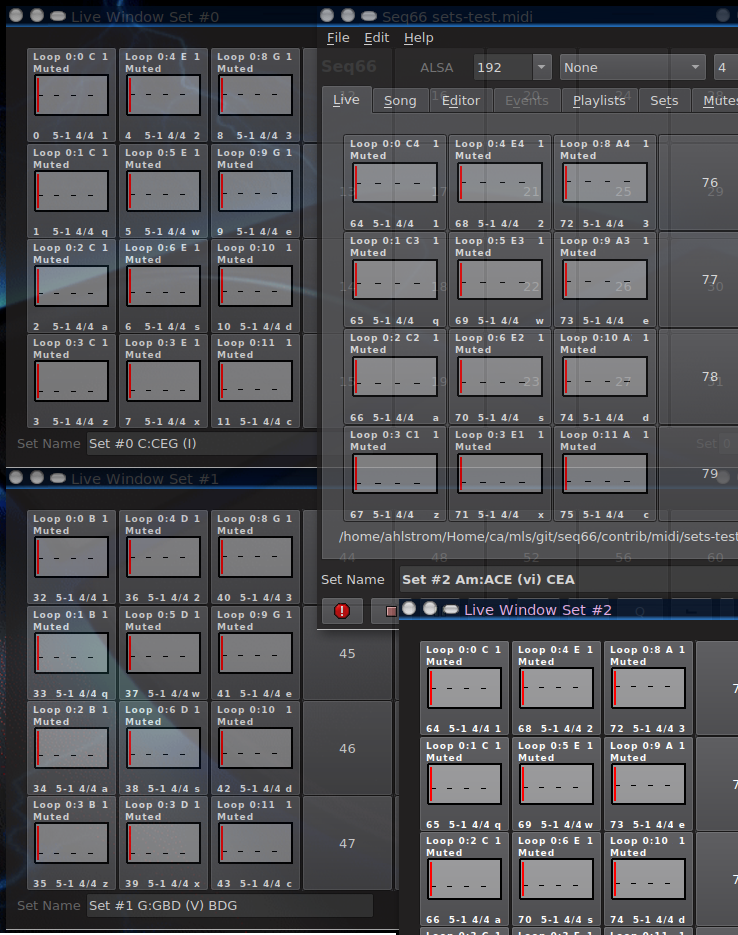
\includegraphics[scale=0.65]{main-window/multiple-live-grids.png}
   \caption{Multiple Live Grids}
   \label{fig:multiple_live_grids}
\end{figure}

   Note that the right-click slot menu has some items removed when the live
   grid is in an external window, or the main window is showing a set other
   than set 0, as indicated by the asterisks in the list below.
%  \textsl{We hope to rectify that in a future release.}

   Once a pattern is created in a slot, there are more
   right-click options for that slot.
   \index{pattern!right click}
   A \textsl{right-click} on a \textbf{slot with a pattern} brings up a menu
   to allow one to edit it, or perform a few other actions
   specified in the context menu.  Here are the menu entries:

% \begin{figure}[H]
%    \centering 
%    \includegraphics[scale=0.65]{main-window/slot-record-toggle.png}
%    \caption{Slot Popup Menu}
%    \label{fig:slot_record_toggle}
% \end{figure}

   The menu for a slot with a pattern is more extensive:

\begin{figure}[H]
   \centering 
   \includegraphics[scale=0.75]{tabs/live/pattern-popup-menu-2.png}
   \caption{Patterns Panel Pop-up Menu}
   \label{fig:patterns_panel_popup_menu}
\end{figure}

   This layout has changed; the entries are nested to save space.

   \begin{enumerate}
      \item \textbf{New pattern}
      \item \textbf{Live grid window for set ...} *
      \item \textbf{Record toggle}
      \item \textbf{Edit}
      \begin{enumerate}
         \item \textbf{Edit pattern in tab} *
         \item \textbf{Edit pattern in window} *
         \item \textbf{Edit events in tab} *
      \end{enumerate}
      \item \textbf{Color}
      \item \textbf{Track}
      \begin{enumerate}
         \item \textbf{Flatten triggers}
         \item \textbf{Export}
         \item \textbf{Copy}
         \item \textbf{Cut}
         \item \textbf{Delete}
         \item \textbf{Clear events}
      \end{enumerate}
      \item \textbf{Merge into pattern}
      \item \textbf{Input Bus}
      \item \textbf{Output Bus}
      \item \textbf{Output Channel}
   \end{enumerate}

   The first menu entry is the same as above.  However, since there is
   already a pattern present in the slot, the user is prompted before erasing
   the current pattern and creating a new one.

   \setcounter{ItemCounter}{0}      % Reset the ItemCounter for this list.

   \itempar{New Pattern}{pattern!new}
   Creates a new pattern in the empty slot.
   \index{slot!double-click}
   A double-click on an empty slot can also be used.

   \itempar{Live grid window for Set}{pattern!external live frame}
   This selection uses the pattern number to open the corresponding screenset
   number in an external \textbf{Live} frame.
   This allows viewing and interacting with a number of sets.

   \itempar{Record Toggle}{pattern!record toggle}
   Selecting this item toggles the recording status of the pattern.
   If the grid record mode button shows something other than
   \textbf{None} (e.g. \textbf{Quantize}), then that alteration is supplied.
%  (The loop-record style is not applied at this time. TODO).
   Note that recording can also be set in the pattern editor, or via
   the "record" loop-mode, or by automation.
   (The default key is \texttt{+}; click it and then select the
   desired slot via mouse or hot-key.)

\begin{figure}[H]
   \centering 
   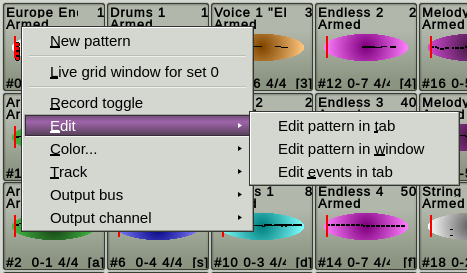
\includegraphics[scale=0.75]{tabs/live/pattern-popup-menu-3.png}
   \caption{Patterns Panel Pop-up Edit Menu}
   \label{fig:patterns_panel_popup_edit_menu}
\end{figure}

   \itempar{Edit Pattern In Tab}{pattern!edit in tab}
   Selecting this item activates the \textbf{Edit} tab and fills it with data
   from the selected pattern.
   Note that this editor is slightly simpler than the external pattern editor
   described just below.

   \itempar{Edit Pattern In Window}{pattern!edit in window}
   Selecting this item brings up the pattern in an external pattern editor that
   has a few addition controls over the \textbf{Edit} tab (where space is more
   constrained).

   In addition to \textsl{right-click} and select \textbf{New}, the user can
   \index{empty slot double-click}
   \textsl{double-click} on the empty slot,
   to bring up a new instance of the sequence
   editor.  For \textsl{double-click} on an existing pattern,
   the effect can be a bit confusing at first,
   because it also toggles the armed/muted status of the slot
   quickly twice (leaving it as it was).

   \index{editing shortcut}
   \index{keys!=}
   \index{keys!pattern edit}

   A nice feature is hitting the equals ("=") key, then hitting
   a pattern shortcut key (hot-key), to bring up a new sequence or edit an
   existing one in a \textbf{Pattern Editor} .

   \itempar{Edit Events In Tab}{pattern!events in tab}
   Edits an existing loop or pattern, but using a detailed \textbf{Event Editor}
   tab that shows events as text and numbers, and allows editing them as text
   and numbers.
   This editor is basic, meant for viewing
   MIDI events and making some minor edits or deletes.
   The \textbf{Event Editor} is most useful when trying to find events
   that are screwing up the performance of that pattern.
   See \sectionref{sec:event_editor}, for more information.

   \index{keys!-}
   \index{keys!event edit}
   Another feature is hitting the minus
   ("-") key, then the hot-key, to bring up the \textbf{Event Editor} tab.
   The configuration file settings for the the '=' and
   '-' keys can be altered in the 'ctrl' file.

   \itempar{Pattern Color}{pattern!color}
   Opens a menu to select a color for the pattern.  This selects a color
   palette value (index) into the currently loaded color palette.
   32 palette colors are supported, and the palette can be modified.
   See \sectionref{sec:palettes}.

\begin{figure}[H]
   \centering 
   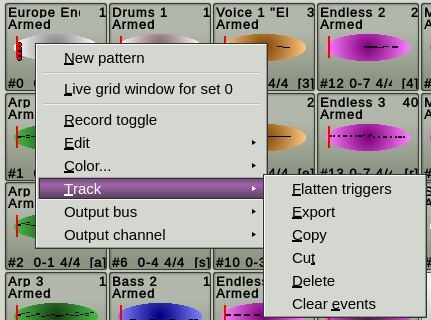
\includegraphics[scale=0.75]{tabs/live/pattern-popup-menu-5.png}
   \caption{Patterns Panel Pop-up Track Menu}
   \label{fig:patterns_panel_popup_track_menu}
\end{figure}

   \itempar{Flatten}{pattern!flatten}
   This item "flattens" a sequence that has triggers.
   This means that the triggers are used to create the events without
   the triggers, so that the track can be used in MIDI sequencers that
   do not support \textsl{Seq66} triggers.
   However, one trigger is created for the whole track, for potential
   future editing in \textsl{Seq66}.
   Other sequencers should simply ignore this trigger.

   \itempar{Export}{pattern!export pattern}
   This operation takes the current track, in whatever form it is (SMF 0, 1,
   and with or without triggers), and writes it to a new
   MIDI file in pattern zero (MIDI track 1).
   This makes it easy to import the track into many different tunes.
   (In future release, perhaps a destination track number will be
   specifiable....)

   \itempar{Copy}{pattern!copy}
   Copies the pattern underneath the mouse cursor.
   The pattern can then be pasted elsewhere in the Patterns panel.
   One can also drag-and-drop a pattern into another cell (there is no outline
   box during the drag, unfortunately).
   See \sectionref{subsubsec:patterns_pattern_slot}.
   Note that there is no \texttt{Ctrl-C} key for this operation in the
   live (main) window.

   \itempar{Cut}{pattern!cut}
   Cuts the pattern while copying it for later pasting.
   There is no \texttt{Ctrl-X} key for this operation.

   \itempar{Delete}{pattern!delete}
   Deletes the pattern.  Currently the same as Cut!

   \itempar{Clear events}{pattern!clear}
   This selection leaves the pattern and its specifications in place,
   but removes all events from the pattern.

   \itempar{Paste Pattern}{pattern!paste}
   Pastes a loop or pattern that was previously copied.
   This option is shown only when
   \textsl{right-clicking} over an empty pattern.
   It causes a cut or copied pattern to be replicated into the emptly slot.
   Note that there is no \texttt{Ctrl-V} key for this operation in the
   main window.
   Also note that the pattern clipboard can be pasted after a
   \textbf{File / New} or \textbf{File / Open},
   to copy it to another file.

   \itempar{Merge Into Pattern}{pattern!merge}
   Like \textbf{Paste to pattern}, it pastes a
   patten that was cut or copied into the pattern slot where the mouse was
   \textsl{right-clicked}.  However, the original notes remain.  Thus, the merge
   option provides a way to build up a pattern by copying other patterns.

   \itempar{Output Bus}{pattern!buss}
   This item allows one to select the output buss for a pattern without having
   to open the editor.
   Note that having an output buss setting for a pattern is mandatory.
   The output buss is stored as a simple buss number ranging from 0 on up to
   the number of MIDI output devices.

   \itempar{Output Channel}{pattern!channel}
   This item allows one to select the output channel for a pattern without
   having to open the editor.

\begin{figure}[H]
   \centering 
   \includegraphics[scale=0.65]{main-window/slot-inputt-buss.png}
   \caption{Input Bus Popup Menu}
   \label{fig:slot_input_bus}
\end{figure}

   \itempar{Input Bus}{pattern!input buss}
   \textsl{Seq66} supports an
   \textsl{optional} input buss setting for each pattern.
   This setting is not available in the pattern editor due to lack
   of room, so this popup menu is the only way to get to this option.
   Normally, the "current" pattern, which is the one opened in
   the pattern editor, is the only one accepting input when
   recording is activated.

   By setting an input buss, incoming MIDI events can be routed to
   the pattern that is set to accept input from that buss.
   As the figure shows, the full set of input ports is shown.
   Some are disabled. (The "ALSA Announce" buss, should be disabled; this
   is a bug.)

   In the figure, the "Input B" pattern will accept events from
   the \textsl{KORG nanoKEY2} keyboard.
   If the \textbf{Free} entry is selected (the default), then
   the pattern will accept input from any MIDI input port.

   \textbf{Important}:
   \begin{itemize}
      \item If a MIDI input device is not enabled in the port list,
         it will not work as an input buss.
      \item If a MIDI input device is defined as an automation controller for
         \textsl{Seq66}, it will not work as an input buss.
      \item To disable the usage of input-buss routing, set the input buss
         to \textbf{Free} for all patterns, then save and reload the file.
      \item To record normally to a pattern, open the pattern for recording
         and use a MIDI device that has \textsl{not} been assigned as
         a pattern's input buss.
   \end{itemize}

   One final note... the input buss setting overrides the record-by-channel
   setting.

\paragraph{Pattern Labels}
\label{paragraph:patterns_labels}
   
   A \textbf{filled pattern slot} is referred to as a \textsl{pattern}
   (or \textsl{track}, \textsl{loop}, or \textsl{sequence}).
   A pattern is shown in the pattern grid as a filled slot with a number of
   labels surrounding it.  Here are the labels shown:

   \begin{itemize}
      \item \textbf{Pattern Name}. Top left.
         \index{pattern!name}
         This line, in the upper left of the pattern slot, contains the name or
         title of the pattern, for reference when juggling a number of
         patterns.
      \item \textbf{Pattern Status}. Second line.
         \index{pattern!status}
         Underneath the pattern-name is the status of the pattern, such as
         "New" (untitled with zero events), "Armed", "Muted", or "Queued".
         This status is useful when the Qt theme coloring makes the exact
         status difficult to determine.
      \item \textbf{Pattern Length}. Top right.
         \index{pattern!length}
         The length of the pattern, in measures, is shown in the upper
         right corner of the pattern slot.
         If the pattern has been modified, an \textbf{asterisk}
         appears after the
         number.
         Otherwise, if the loop-count for the pattern is greater than 0, 
         then an \textbf{plus sign} is shown.
         Remember that a pattern loop-count of 0 means the pattern can repeat
         "forever".
      \item \textbf{Notes or Fingerprint}. Center progress box.
         \index{pattern!contents}
         The contents of the pattern, in the central box,
         provide a distinguishable representation of the notes or events in the
         pattern.
         The notes are shown in the center, inside a "progress box" that
         can also be colored, or not shown at all.
         Long patterns can be replaced by a much shorter "fingerprint", for
         faster drawing.
         Tempo events are indicated by a small circle.
         \index{empty pattern}
         An pattern with no playable events will not needlessly scroll
         during playback.
         However, if a pattern has even a single event (say, a program change),
         it will scroll.
      \item \textbf{Progress Cursor}. Center.
         At the left of each center box is a vertical line, waiting for
         playback to start so that it can move through the pattern, again and
         again.
         When the song is playing, this vertical bar
         tracks the position of the playback of the pattern or loop; it
         returns to the beginning of the box every time the pattern starts
         over.
      \item \textbf{Sequence Number}. Bottom left.
         This number is shown at the bottom left of the pattern slot.
         Pattern numbers, by default, range from 0 to 1023.
         Note how it varies fastest by row (top to bottom).
         There is a configuration item to change transpose them.
      \item \textbf{Bus-Channel}. Bottom, second from left.
         \index{pattern!bus-channel}
         This pair of numbers shows the the MIDI buss number, a dash, and
         the MIDI output channel number.
         For example, "0-2" means MIDI buss 0 (re 0), channel 2 (re 1).
         \index{pattern!free channel}
         If the channel is an "F", this means that the pattern has no specified
         output channel, and can play on all channels.
         This "free" channel concept is useful for applying Program Changes and
         Volume controls to many channels at once.
      \item \textbf{Beat/Beat Width}. Bottom, third from left.
         \index{pattern!beat}
         This pair of numbers is the standard time-signature of the pattern,
         such as "4/4" or "3/4".  The first number is the beats-per-measure,
         and the second is the size of the beat, here, a quarter note.
      \item \textbf{Shortcut Key}.  Also known as the
         \textbf{hot key}, this symbol is shown at the bottom right of the
         slot, in square brackets for better visibility.
         The key noted in the lower-right corner of the pattern is a "hot-key"
         that can be pressed to toggle the mute/unmute status of that pattern.
         This action is an alternative to
         \textsl{left-click} on the pattern.
         This hot-key can also be used to open the pattern in a pattern editor
         or in the event editor.
         Other actions are supported by changing the 
         \textbf{loop mode}.
      \item \textbf{Armed}. Highlight color of button.
         Button highlighting indicates that the pattern is armed
         (unmuted), and will play if playback is initiated in the pattern
         \index{live mode}
         window in live mode.
         An item is armed/disarmed by a
         \textsl{left-click} on it, or by using the
         button's hot-key.
      \item \textbf{External Frame}. \textsl{Shift-left-click}.
         \index{shift left click}
         If the \texttt{Shift} key is held during a
         \textsl{left-click} on a pattern,
         the corresponding set's \textbf{Live} frame is brought up.
   \end{itemize}

   \index{pattern!left click}
   \textsl{Left-click} on an filled pattern box will toggle the status of the
   pattern between muted (white background) and unmuted (black background).
   If the song is playing via the main window, toggling this status makes
   the pattern stop playing or start playing.  The armed status
   can also be toggled using hot-keys and MIDI controls.

\subsubsection{Basic Pattern Control}
\label{subsubsec:patterns_basic_pattern_control}

   In addition to the arm/mute function done by clicking on a pattern slot,
   there are some additional controls that can be enabled on the fly:

   \begin{itemize}
      \item \textbf{Queue}.
         Enables one pattern to be turned on or off as soon as the pattern
         loops to its beginning.
      \item \textbf{Keep-queue}.
         The same as Queue, but stays active until disabled.
      \item \textbf{Oneshot}.
         Similar to Queue, but it merely unmutes a pattern for one cycle,
         then mutes it.
      \item \textbf{Replace}.
         Soloes a pattern immediately.
         Can be repeated many times.
         Then restores the original status of patterns.
      \item \textbf{Solo}.
         Similar to Replace, but the process is queued.
      \item \textbf{Snapshot}.
         Similar to Queue, but arms a pattern, plays it once, and turns it
         off.
      \item \textbf{Learn}.
         Maps a set of pattern arm/mute statuses to a keystroke.
   \end{itemize}

   These actions are described in detail below.
   They have some common preconditions and indicators that are listed here:

   \begin{itemize}
      \item \textbf{Live mode}.
         Make sure that the song is in \textbf{Live} mode.
      \item \textbf{Playback}.
         These features work best with playback already started.
      \item \textbf{Enabled patterns}.
         Make sure that some patterns are armed.
         In some cases, a snapshot of them is saved.
      \item \textbf{Status indicator}.
         When a control-mode is activated, a status indicator appears, with
         italics text indicating the status. It appears between the
         file-name and the Metronome button.
   \end{itemize}

   The keystrokes noted are mentioned in
   \sectionref{paragraph:patterns_pattern_keys}.

\paragraph{Pattern Queue}
\label{paragraph:patterns_pattern_queue}

   Pressing the "queue" key and then hitting a pattern hot-key
   will queue an on/off toggle for a pattern when the end of the loop is
   reached.
   This means that the change in state of the pattern will not take hold
   immediately, but will kick in when the pattern loops back to its beginning.
   This pending state is indicated by coloring the central box of the
   pattern grey.
   Also check out the "keep queue" functionality and
   the "one-shot queue" functionality described below.

   \begin{enumber}
      \item Press \texttt{o}; note that a "Queue" status indicator appears.
      \item Click a pattern.
      \item It is queued for arm or queued for mute (the opposite of its
         original status).
      \item It is in effect for only one pattern click, then must be
         reestablished, if desired, by going back to step 1.
   \end{enumber}

% This is something to look into. Doesn't seem to work at all. Does it
% work in Sequencer64.
%
%  Queue also works for mute/unmute pattern sets ("groups"); in this case,
%  every sequence will toggle its status after its individual loop ends. 

\paragraph{Pattern Keep-Queue}
\label{paragraph:patterns_pattern_keep_queue}

   Pressing the "keep queue" hot-key activates a "sticky" queue mode.
   In this mode, pressing a pattern key immediately turns on queuing.
   Multiple patterns can be handled serially in this way;
   keep-queue persists until one clicks the queue hot-key again,
   or changes the active (viewed) screen-set. 
   \index{queue!cancel}
   Keep-queue” is cancelled by pressing the keep-queue hot-key again.
   There is also a \textbf{Q} button in the main window
   for the same purpose.
   Also note the "queued replace/solo" functionality, described a bit later.

   \begin{enumber}
      \item Press the backslash; note that a "Keep Q" status indicator appears.
      \item Click a pattern.
      \item It is queued for arm or queued for mute (opposite of original status)
      \item It is in effect for all pattern clicks until the keep-queue key
         is pressed again.
         The "Keep Q" status indicator disappears.
   \end{enumber}

\paragraph{Pattern Oneshot}
\label{paragraph:patterns_pattern_oneshot}

   Thanks to \textsl{Kepler34}, we have "one-shot queue"
   functionality.  This one-shot setup queues a pattern up for unmuting only,
   and, once the pattern has played, it is automatically muted.  This process
   is easier than having to unqueue the pattern manually before the next
   playback.

   A light-grey color is used to show a "one-shot" queue.
   The one-shot queue can only turn a pattern on, and it
   will force the pattern off after one play.

   \begin{enumber}
      \item Press the pipe key; note that a "Oneshot" status indicator appears.
      \item Click a pattern.
      \item It is queued for arm only.
      \item It plays once, and then stops.
         The "Oneshot" status indicator disappears automatically.
   \end{enumber}

\paragraph{Pattern Replace}
\label{paragraph:patterns_pattern_replace}

   The "replace" automation key/control sets a form of muting/unmuting.
   When the "replace" hot-key is
   pressed, and then a pattern's hot-key is pressed,
   that sequence is unmuted, and all of the other sequences are muted.
   Other patterns can be clicked to be armed/muted; when the "replace" hot-key
   is clicked again, the original patterns armed before the first "replace"
   click are restored.
   "Replace", like other controls, is also implemented via MIDI control,
   where the MIDI control can be activated; but then the user has to select
   the desired sequence.  

   \begin{enumber}
      \item Press 0; note that a "Replace" status indicator appears.
      \item Click a pattern; it either stays on or is turned on.
      \item All other patterns are saved as a snapshot, then are immediately
          muted (no queuing).
      \item More patterns can be soloed by clicks.
      \item Press 0 again, and the original patterns (snapshot) are restored.
          The "Replace" status indicator disappears.
   \end{enumber}

\paragraph{Pattern Solo}
\label{paragraph:patterns_pattern_solo}

   \textsl{Seq66} provides an extension to the replace functionality
   that is called "queued-replace" or "queued-solo".
   In this feature, the "keep queue" function is activated and the
   replace function is queued so that it does not occur until the next
   time the patterns loop.
   And queued-replace provides a form of snapshot, limited to the
   \textsl{current} screen-set.
   Here are the steps:

   \begin{enumerate}
      \item Be careful which key, "BS" (\texttt{Ctrl-H})
         or "BkSpace" (\texttt{Backspace}), is configured.
         They are two different keystrokes. "BkSpace" 
         is to be preferred and is the default.
      \item Start playback with some patterns on. 
      \item Press and release
         the "solo" hot-key.  This puts the application into
         "queued replace" mode.
         It is indicated via a highlighted "\textbf{Q}" button
         and a "Solo" status indicator.
      \item Click the desired pattern hot-key.  Observe that it arms or
         stays on, and that the other playing patterns show the "queued" color
         (grey).  At the end of the loop, they turn off, and the "replace"
         pattern is now soloed.
         This step can be repeated with other patterns.
%     \item Click the same pattern hot-key again. Observe that the other
%        patterns that were toggled off are now queued to be toggled on at the
%        next loop.  Step 4 can be repeated endlessly.
      \item To end
         \index{queue!clear}
         \index{queue!end}
         the "queued-replace" mode, click the "solo" hot-key.
         This restores the original statuses of the patterns.
         Also, changing the active screen-set ends "queue-replace"
         mode.
% Make sure this works:
% It does \textsl{not} end normal queue mode, to preserve the
%        behavior found in \textsl{Seq24}.
%        One needs to clear the queue mode in order to select another pattern
         to solo.
   \end{enumerate}

\paragraph{Pattern Snapshot}
\label{paragraph:patterns_pattern_snapshot}

   When a snapshot key is pressed and released the state of the patterns
   (armed versus unarmed) is saved as a snapshot.
   While the snapshot is in force, one can then change the state of the patterns
   (using keyboard, mouse, or MIDI controls) to change how the song plays.
   When the snapshot mode is exited by pressing the snapshot key again, the
   original saved state of the patterns is restored.

   \begin{enumber}
      \item Press \texttt{Ins}; note that a "Snapshot" status indicator appears.
      \item The first press of Ins saves the current state of the patterns.
      \item The user can mute/unmute any combinations of patterns.
      \item The next press of \texttt{Ins} restores the snapshot.
         The "Snapshot" status indicator disappears.
      \item The snapshot "buffer" is cleared to get ready for the next
         \texttt{Ins}.
      \item Snapshot mode is non-queued.
   \end{enumber}

\paragraph{Pattern Learn}
\label{paragraph:patterns_pattern_learn}

   Learn is activated by the \texttt{l} (lower-case L) key or the "L"
   button.
   Once activated, the next pattern hot-key (lower-case) pressed will
   cause the current set of armed/muted patterns in the screen-set to be
   stored with the upper-case (shifted) version of that hot-key.
   See \sectionref{subsubsec:introduction_mute_group_learn_button}.

\subsubsection{Pattern Keys and Clicks}
\label{subsubsec:patterns_pattern_keys_and_clicks}

   This section recapitulates all the clicks and keys that perform actions
   in the Pattern windows.  Some additional clicks and keys are noted here
   as well.
   Also refer to \sectionref{sec:kbd_mouse_actions}.

\paragraph{Pattern Keys}
\label{paragraph:patterns_pattern_keys}

   \index{keys!hot}
   \index{keys!shortcut}
   Each pattern in the patterns panel can have a hot-key or shortcut-key
   associated with it.

   \index{keys!pattern toggle}
   \textbf{Pattern Toggle}.
   Like a \textsl{left-click}, for each pattern, its assigned hot-key will
   also toggle its status between muted/unmuted (armed/unarmed).
   Here is the normal layout of patterns, which was built into
   \textsl{Seq24}'s "DNA":

   \begin{verbatim}
      [  0 ] [  4 ] [  8 ] [ 12 ] [ 16 ] [ 20 ] [ 24 ] [ 28 ]
      [  1 ] [  5 ] [  9 ] [ 13 ] [ 17 ] [ 21 ] [ 25 ] [ 29 ]
      [  2 ] [  6 ] [ 10 ] [ 14 ] [ 18 ] [ 22 ] [ 26 ] [ 30 ]
      [  3 ] [  7 ] [ 11 ] [ 15 ] [ 19 ] [ 23 ] [ 27 ] [ 31 ]
   \end{verbatim}

   There is an alternate (and fairly new) mapping that can be enabled
   using the \texttt{swap-coordinates} option in the 'usr' file.
   See \sectionref{subsubsec:usr_file_user_interface_settings}.
   Below is the default keyboard "grid" that is
   mapped to the loops/patterns on the screen-set.

   \begin{verbatim}
      [ 1 ][ 2 ][ 3 ][ 4 ][ 5 ][ 6 ][ 7 ][ 8 ]
      [ q ][ w ][ e ][ r ][ t ][ y ][ u ][ i ]
      [ a ][ s ][ d ][ f ][ g ][ h ][ j ][ k ]
      [ z ][ x ][ c ][ v ][ b ][ n ][ m ][ , ]
   \end{verbatim}

   These characters are shown in the lower right corner of each
   pattern, as an aid to memory.
   This grid can be changed in the 'ctrl' file in the
   \texttt{[loop-control]} section.
   However, it is best to leave this setup as is, except for the key-swapping
   needed for alternative keyboard layouts like "QWERTZ".

   \index{keys!pattern shift}
   \textbf{Pattern Shift}.
   A "shift" functionality is available for the
   mute/unmute hot-keys when a set is larger than 32 patterns.
   \index{keys!slash}
   \index{variset!slash key}
   Normally, pressing the \texttt{1} key will toggle
   sequence 0.  If preceded by one slash key (\texttt{/}), then sequence 32
   will be toggled.  If preceded by two slash keys, then sequence 64 will be
   toggled.  This features supports using set sizes of 32, 64, and 96 patterns.

   \index{keys![}
   \index{keys!decrement set}
   \index{keys!screenset down}
   \textbf{Screenset Increment and Decrement}.
   The "\texttt{[}" and
   \index{keys!]}
   \index{keys!increment set}
   \index{keys!screenset up}
   "\texttt{]}" keys on the keyboard decrement or increment the set number.

   \index{keys!alt}
   \index{keys!snapshot}
   \textbf{Snapshot}.
   Unlike in \textsl{Seq24}, the \texttt{Alt} keys are not used for snapshots.
   In addition, the snapshot key acts like a \textsl{toggle}...
   no need to hold it down.
%  Lastly, there is only one snapshot key slot.
   It's best to use something that does not trigger desktop/window
   commands; the default key is \texttt{Ins}.
   Configured in the 'ctrl' file \texttt{[automation-control]} section.

   \index{keys!right ctrl}
   \index{keys!queue}
   \index{queue!temporary}
   \index{keys!avoid ctrl/alt}
   We do \textbf{not}
   recommend using \texttt{Ctrl} or \texttt{Alt}
   keys for pattern control.  They conflict with application or desktop
   settings.
   The default queue key is \texttt{o} (lower-case O).

   \index{keys!keep queue}
   \index{queue!keep}
   The default keep-queue key is the \texttt{Backslash}.

   \index{one-shot queue}
   \index{keys!one-shot queue}
   \index{queue!one-shot}
   The default one-shot queue key is \texttt{|}, the pipe character.

   \index{keys!replace}
   The default keep-queue key is \texttt{Keypad Home}.

   \index{queue!solo}
   The default solo key is \texttt{Backspace}.

   \begin{comment}


   Before pressing the "keep queue" key, patterns 33 ("\textbf{q}")
   and 34 ("\textbf{a}") are
   unmuted, while the desired replace pattern, 32 ("\textbf{1}") is off.
   Then the user presses (and holds) the "replace" key, then clicks the
   "\textbf{1}" key.
   This puts all unmuted patterns, plus the muted
   replace pattern as well, into queue mode, as shown by the grey panels.
   When the progress bar reaches the end of the pattern, pattern 32 will go on,
   and patterns 33 and 34 will go off.
   If the replace-pattern is already on, it is not queued, as
   there's no need to turn it on.

   If, while in queue mode, the replace key is held and
   "\textbf{1}" is pressed again,
   the other patterns will be queued, and will turn on again.  Thus, the
   solo status of the replace pattern can be toggled at will, until queue mode
   is exited by pressing and releasing the normal "queue" key.
   If the replace key is \textsl{not} held down, and another pattern's replace
   hot-key is pressed, that pattern will be queued normally.
   If one wants to change the solo functionality to a different pattern,
   simple hold the replace key and click on a different pattern.  The new
   arrangement of soloing is memorized.
   One can clear the queue mode by pressing the normal queue key.

   \end{comment}

   There are more keys defined in the 'ctrl' file, and it is
   worth figuring out what they do, if not documented here.
   Also see the installed \texttt{control\_keys.ods} spreadsheet.
   For a couple of short, but good, video tutorials about using arming,
   queuing, and snapshots in \textsl{Seq24}, see reference \cite{wootangent1}.

\paragraph{Other Pattern Clicks}
\label{paragraph:patterns_pattern_clicks}

   \index{pattern!left click}
   \index{pattern!mute toggle}
   \textsl{Left-click} on a pattern-filled box will change its state
   \index{pattern!mute}
   \index{pattern!unmute}
   from muted (white background) to playing (black background), whether
   the sequencer is playing or not.

   \index{pattern!left click-drag}
   \textsl{Left-click-hold-drag} on a pattern, drags it to a different
   pattern on the grid.
   The box disappears while dragged, and reappears in the new location when
   dropped.  However, a pattern \textsl{cannot} be dragged if its
   \textbf{Pattern Editor} window is open.

   \index{pattern!right click}
   \textsl{Right-click} on a pattern brings up the appropriate context menus, as
   discussed earlier, depending on whether the pattern box is empty or
   filled.

   \index{pattern!middle click}
   \textsl{Middle-click} on a pattern will bring up the pattern
   in the \textbf{Editor}
   tab in the main window.

   \index{pattern!shift-left-click}
   \index{shift-left-click live-frame}
   \textsl{Shift-left-click} on a pattern will open up an external
   live-frame for the
   set having the same number as the pattern.

   \index{pattern!ctrl-left-click}
   \index{ctrl-left-click new pattern}
   \textsl{Ctrl-left-click} on a pattern will create a new pattern, just like
   double-click will (if enabled).

   \index{solo!true}
   \index{pattern!alt-left-click}
   \index{patterns panel!inverse muting}
   \index{patterns panel!solo}
   \index{alt-left-click solo}
   There is a truer "Solo" functionality in the Patterns
   Panel and the Song Editor.  To "solo" a pattern, move the mouse cursor
   over the pattern, hold the \texttt{Alt} key, and left-click the pattern.
   This will turn off all the other patterns, so that the selected pattern ins
   the only one playing.
   Also see \sectionref{paragraph:patterns_loop_modes}; it notes another way to
   solo a pattern.

   One thing to remember with solo is that it can be reversed (reenabling all
   the other patterns) only if that same pattern is clicked. Soloing another
   pattern will lose the list of previously-enabled patterns.

\paragraph{Metronome}
\label{paragraph:patterns_metronome}

   \index{metronome}
   Also shown in the figure is a \textbf{Metronome} button.
   This is a feature new with \textsl{Seq66} version 0.99.0, and still has a few
   minor issues to work out, but it works.
   The metronome has a number of configurable items.
   See \sectionref{subsubsec:configuration_rc_metronome}.

   Clicking the metronome button turns the metronome on and off.
   To use the metronome (once configured), click the button to enable it,
   then start playback.
   It can be turned on and off during playback.
   It is always available, stored as a hidden automatically-generated
   pattern.

\paragraph{Count-in Recording}
\label{paragraph:patterns_background_recording}

   \index{count-in recording}
   Also shown in the figure is a \textbf{Count-In Recording} button.
   This feature still has a few
   minor issues to work out, but it works.
   It is not \textbf{background recording}, which involves a
   thread continuously recording in the background.  Some day.

   The recorder has a number of configurable items.
   See \sectionref{subsubsec:configuration_rc_background_recording}.
   Count-in recording needs to be enabled in the configuration.
   Otherwise, the count-in-recording button is disabled.

   When enabled, press the count-in-recording button.  Now all events on the
   given input buss will be recorded, even if playback is not started.
   Better to start playback after enabling recording!

   Once one is satisfied with the recording, stop playback, then
   click the count-in-recording button again.
   If any events have been recorded, then they are pasted into a new pattern in
   the next available pattern slot.
   There, they can be edited or deleted.
   Note that the count-in pattern is muted while recording.
   We will change how it works based on user feedback.

\paragraph{Pattern Loop-Record Modes}
\label{paragraph:patterns_loop_modes}

   \textsl{Seq66} has always had the feature of turning on recording,
   including quantized recording, in the pattern editor.
   Now, it also provides for
   \index{loop!grid modes}
   loop-grid modes.
   With this feature, the normal loop muting/unmuting
   functionality of the \textbf{Live Grid} buttons
   can be changed to allow the toggling
   of recording or other actions to be applied to the affected  pattern.
   This new functionality is enabled by two buttons in the main window grid and
   by two refactored keystroke/MIDI controls ("Record" and "Quan Record").
   The normal mode (mute/unmute) is called \textbf{Loop}.

   \begin{itemize}
      \item \textbf{Loop}.
         This mode is the legacy and long-time standard mode of
         \textsl{Seq24}, \textsl{Sequencer64}, and \textsl{Seq66}.
         When in this mode, a click on a pattern slot, a loop-control
         keystroke, or a loop-control MIDI event will change the mute/unmute,
         armed/unarmed status of a pattern.
      \item \textbf{Record}.
         A click/key on the pattern turns on recording for that pattern.
         This status is shown by the appearance of a red circle in the pattern
         button.
      \item \textbf{Copy}.
         Copies the selected pattern into the clipboard.
      \item \textbf{Paste}.
         Pastes the clipboard into the selected pattern.
      \item \textbf{Clear}.
         Removes the events from the selected pattern.  Careful!
      \item \textbf{Delete}.
         Deletes the selected pattern.  Careful!
      \item \textbf{Thru}.
         Turns on the MIDI Thru functionality of the selected pattern.
      \item \textbf{Solo}.
         Soloes the selected pattern.
      \item \textbf{Cut}.
         Deletes the selected pattern and copies it into the clipboard.
      \item \textbf{Double}.
         Doubles the length of the selected pattern.
   \end{itemize}
   It has been supplemented by four recording modes.
   Here are the modes:

   \begin{itemize}
      \item \textbf{Overdub}.
         \index{merge}
         \index{overdub}
         \index{record!merge}
         \index{record!overdub}
         Also known as \textbf{Merge},
         this mode is selected by clicking on the \textbf{Loop} button,
         then using the \textbf{Record} control.
         These commands cycle between all the modes in this list.
         Overdub is the same as the \textbf{Merge} option in the 
         pattern editor.
         Clicking a grid will turn on/off the overdub recording mode
         for that pattern.
         It enables recording that accumulates note events in each pass of
         looping through the pattern.
      \item \textbf{Overwrite.}
         \index{overwrite}
         \index{recording!overwrite}
         This mode causes the grid button to turn on overwrite recording.
         When the loop restarts over and a note is pressed,
         then the existing notes in that loop are erased,
         and the new note is added.
      \item \textbf{Expand}.
         \index{expand}
         \index{recording!expand}
         This mode causes the grid button to turn on expand recording.
         Once the end of the loop is near, whether or
         not any notes are being input, another measure is added to the length
         of the loop.
      \item \textbf{One-shot}.
         \index{one-shot}
         \index{recording!one-shot}
         When this option is set, with the record button on, and no pattern
         playing, recording won't start until a note comes in, and when the
         first note comes in, the progress bar starts at the left (time 0).
         As each new set of notes at the same timestamp come in, the
         notes are recorded and the current time advances by one snap value.
         Once the end of the pattern lenght is reached, recording is turned
         off.
      \item \textbf{One-shot Reset}.
         \index{one-shot reset}
         \index{recording!one-shot reset}
         When the \textbf{One-shot} option is selected, this new option
         is enabled.
         When clicked, three things happen:
         \begin{itemize}
            \item One-short counters/flags are \textsl{reset}.
            \item Recording is turned \textsl{back on}.
               Thus, one can easily re-do a one-shot recording.
            \item The (note) events just recorded are \textsl{no longer
            erased}. Instead, one can use the slot popup menu entry
            \textbf{Clear events}.
            This seems safer, if slightly clumsy.
         \end{itemize}
   \end{itemize}

   These loop-record modes are automatically applied if a pattern is opened
   in the pattern editor.

   Once the recording mode is turned on, whether here or in the pattern editor,
   then the recording type comes into play.
   The types of alteration that can come into play are set by clicking the
   button at the right labeled "None" until the desired recording mode
   is shown:

   \begin{itemize}
      \item \textbf{None}.
         Incoming events are recorded as is.
         Plain recording, events recorded with timestamps unaltered.
         Indicated by a red circle in the pattern slot.
      \item \textbf{Quantize}.
         When recording, quantize the incoming events.
         Incoming events are quantized to the snap value of the pattern.
         Indicated by a red circle and a "Q" inside it in a pattern slot.
      \item \textbf{Tighten}.
         A weaker version of \textbf{Quantize}.
         Incoming events are partially quantized to the snap value of the
         pattern.
         Indicated by a red circle and a "T" inside it in a pattern slot.
         This mode is accessible only via this recording mode; there
         is no such button in the pattern editor.
      \item \textbf{Note Map}.
         If a 'drums' file has been specified and is active, then
         incoming events are remapped to different notes.
         This feature is useful in transforming the notes of an old
         drum machine into, say, a \textsl{General MIDI} drum kit.
         Indicated by a red circle and an "N" inside it in a pattern slot.
         This mode is accessible only via this recording mode; there
         is no such button in the pattern editor.
   \end{itemize}

   These alterations are automatically applied if a pattern is opened
   in the pattern editor.

\subsection{Patterns / Bottom Panel}
\label{subsec:patterns_panel_bottom}

   The first line of the bottom panel contains the \textbf{Set Name}
   of the current set, which is editable.
   It contains a button with an exclamation point (\textbf{!}), which
   can be used to reset the play-set (the total of all patterns that are loaded
   for playback) to the patterns in the current set.
   The \textbf{Set} spin-box can be used to change the current set.

   \begin{enumber}
      \item \textbf{Set Name}
      \item \textbf{Set Reset}
      \item \textbf{Set}
   \end{enumber}

   \setcounter{ItemCounter}{0}      % Reset the ItemCounter for this list.

   \itempar{Set Name}{pattern!set name}
   Each of the 32 available screen-sets can be given a name by entering it
   into this field.  This name is saved with the MIDI file.

   \itempar{Set}{pattern!set number}
   This spin widget selects the current screen-set.  The values in this
   field range from 0 to 31 (less if the set-size is a larger value),
   and default to 0.

   \itempar{Set Reset}{pattern!set reset}
   \textsl{Seq66} has a new feature whereby multiple sets can play at once.
   This button, an exclamation point, will reset the playback to the patterns
   in the current set.

   The bottom panel of the Patterns window provides way to control the
   overall playback of the song.  It has changed quite a bit over the last few
   versions of \textsl{Seq66}, and we have not yet caught up with the
   diagrams. And the Qt user-interface adds more changes.
   Refer to the diagram of the whole window, for now.
   It has a number of items:

   \begin{enumber}
      \item \textbf{Panic!}
      \item \textbf{Stop}
      \item \textbf{Play and Pause}
      \item \textbf{Record}
      \item \textbf{Loop}
      \item \textbf{Song Record}
%     \item \textbf{Song Record Snap}
%     \item \textbf{Log Tempo}
%     \item \textbf{Record Tempo}
      \item \textbf{Keep-Queue Status}
      \item \textbf{Toggle Song/Live Mode}
      \item \textbf{Tap Tempo}
      \item \textbf{BPM}
   \end{enumber}

   \setcounter{ItemCounter}{0}      % Reset the ItemCounter for this list.

   \itempar{Panic!}{pattern!panic}
   This new button stops the song and sends MIDI Off messages on all notes.

   \itempar{Stop}{pattern!stop}
   The red square button stops the playback of the song and all its patterns.
   \index{keys!esc (stop)}
   The keystroke for stopping playback is the \texttt{Escape} character; it
   stops playback and rewinds to the beginning of the song.
   The \texttt{Space} keystroke will do the same thing if playback is in
   progress; it is effectively a playback toggle key.

   \itempar{Play and Pause}{pattern!Play}
   \index{pattern!Pause}
   The green triangular button starts the playback of the whole song.
   \index{keys!space (play)}
   The keystroke for starting playback is the \texttt{Space} character by
   default.  It also stops playback, also rewinding the song to the beginning.
   \index{pause}
   The Pause button toggles playback without rewinding the song.
   A Pause key (by default, the period) is also defined.

   \itempar{Record}{patterns!record}
   This button is normally disabled.
   Recording is enabled as desired for only one pattern in this mode.
   When record-by-channel is set, this button is yellow.
   This mode allows events to be redirected to the sequence whose number is the
   channel number (0-15) of the event.
   When record-by-buss is set, this button is red.
   This mode allows events to be redirected to the sequence whose number is the
   buss number (0-15) of the event.

   \itempar{Loop}{pattern!loop}
   If this button is active, then the playback will loop
   between the "L" and "R" markers in the pattern editor or the song editor
   time-lines.
   As with the "L" and "R" markers in the pattern editor, this can
   be placed via left and right mouse clicks.
   Note that the "L" and "R" markers can be selected via the keyboard using
   their respective shifted key.  Once selected, the marker can be moved left
   or right using the left and right arrow keys.

   \itempar{Song Record}{pattern!song record}
   Song-recording in \textsl{Seq66} is adopted from the
   \textsl{Kepler34} project.
   This feature takes live muting changes and records them as
   triggers in the \textbf{Song Editor}.
   The default hot-key for this function is \texttt{P}.
   This feature does not honor queuing...
   rather than waiting until the end of the pattern when the queuing takes
   effect, the trigger recording starts immediately.

%  \itempar{Song Record Snap}{pattern!song record snap}
%  This button toggles snapping the beginning and end of a recorded trigger to
%  the nearest beat.  There is no hot-key for this button at this time.
%  And, in fact, at present, song-record snap is alway in force.

   \itempar{BPM}{pattern!BPM}
   The spin widget adjusts the "beats per minute" (BPM) value.  The
   range of this field is from 1 bpm to 600 bpm, with a default value of
   120 bpm.
   Although this field looks editable, it is not.  Most keystrokes
   that are entered actually toggle one of the pattern boxes.
   However, the following keys can also modify the BPM in small increments:
   \index{keys!semicolon}
   The \texttt{semicolon} reduces the BPM;
   \index{keys!apostrophe}
   The \texttt{apostrophe} increases the BPM.
   Also, if one \textsl{right-clicks} on the
   \textbf{Up} button, the BPM advances to its largest
   supported value, and if one \textsl{right-clicks} on the
   \textbf{Down} button, the BPM
   advances to its lowest value.
   MIDI control for this value is also available.
   The precision of the BPM value can be set to 0, 1, or 2
   decimal places, and the increment values for the step size (small)
   or page size (large) of the BPM spinner can be configured in the 'usr' file.

   \itempar{Tap Tempo}{pattern!tap tempo}
   This control is clicked in time with a tune, to set the
   tempo based on the tempo of the clicks.  Once clicked, the label of this
   button increments with every click, and the \textbf{BPM} field updates to
   display the calculated tempo.  If the user stops tapping for 5 seconds, the
   label reverts to 0, the BPM value keeps its final value, and the user can
   try tapping the tempo again, or accept the current value.
   Tapping can also be done using the keystroke defined
   in the 'ctrl' file.
   It defaults to the "\texttt{F9}" key.

   \itempar{Keep-Queue Status}{pattern!keep-queue}
   This item is the \textbf{Q} button.
   It provides a visual way to know the current state of keep-queue, and is
   activated either by clicking on it or by pressing the assigned keep-queue
   key.

   \itempar{Toggle Song/Live Mode}{pattern!song/live}
   Pressing this button toggles between the song mode and live mode.
   Note that the default mode is configurable, and \textsl{Seq66} can go into
   song mode when a loaded MIDI file has triggers, if configured to do so.

\subsection{Patterns / Multiple Panels}
\label{subsec:patterns_panel_multiple}

   Multiple patterns-panels can be created in addition to the one in the "Live"
   tab.  The live set-up and set-down keystrokes, as well as their MIDI control
   counterparts (both defined in a 'ctrl' file).
   apply only to the main window.

\subsection{Patterns / Variable Set Size}
\label{subsec:patterns_panel_variset}

   \index{variset}
   This option, informally known as "variset", allow some changes in
   the set size and layout from the default 4x8 = 32 sets layout.
   The row count can be set from 4 to 8, and the column count can be set to 8
   to 12.  Note that the set size can only be \textsl{increased} by these
   settings.

   \textbf{Warning:}
   \textsl{seq24} was fairly hardwired for supporting 32 patterns per
   set, and there are still places where that is true.  Thus,
   consider this option to be experimental.

   The \texttt{-o sets=8x8} option can be used to set this mode.
   These settings can be made permanent in the 'usr' file.
   In that file, the options modified are \texttt{mainwnd\_rows} and
   \texttt{mainwnd\_cols}.

   Generally, it is recommend to stick with the 4x8 (32 patterns/set),
   8x8 (64 patterns/set), and 8x12 (96 patterns/set).  This works best with the
   existing set of 32 hot-keys.

   Also note that the Qt 5 user-interface also supports "variset", whether in
   the main window or in the external live-frame.  In addition, the Qt windows
   can be resized and still show reasonable renditions of the pattern-slots.

\subsection{Patterns / Set Handling}
\label{subsec:patterns_panel_set_handling}

   Let's go through an example using the \texttt{Home} key (or whatever key is
   configured as the \textbf{Set Playing Screenset} key.)

   \begin{enumber}
      \item Load a song with more than one screen-set.
      \item Unmute the pattern(s) in the first set and start playback.
      \item Use the "\texttt{]}" (\textbf{Screenset Up}) key to move to the next
         set.  Note that the first set is still playing.  Also note that the
         now-current set is \textsl{not} playing.
      \item Press the \texttt{Home} key.
         Note that the first set turns off, and the current set turns on.
         These steps can be repeated at will.
      \item Finally, hit the \texttt{F8} (\textbf{Toggle Mutes}) key.
         Note that all tracks on all sets toggle muting each time this key is
         pressed.
   \end{enumber}

%-------------------------------------------------------------------------------
% vim: ts=3 sw=3 et ft=tex
%-------------------------------------------------------------------------------


% Pattern Editor

-------------------------------------------------------------------------------
% pattern_editor
%-------------------------------------------------------------------------------
%
% \file        pattern_editor.tex
% \library     Documents
% \author      Chris Ahlstrom
% \date        2015-08-31
% \update      2025-06-06
% \version     $Revision$
% \license     $XPC_GPL_LICENSE$
%
%-------------------------------------------------------------------------------

\section{Pattern Editor}
\label{sec:pattern_editor}

   The \textsl{Seq66} \textbf{Pattern Editor} can edit and preview a
   pattern, configure its buss, channel, transpose, musical
   scale, and many other settings.
   A slightly trimmed version of the \textbf{Pattern Editor} appears in the
   \textbf{Edit} tab in the main window; some controls are hidden and the data
   pane is vertically compressed.
   The full version can be brought up in an external window.

\begin{figure}[H]
   \centering 
   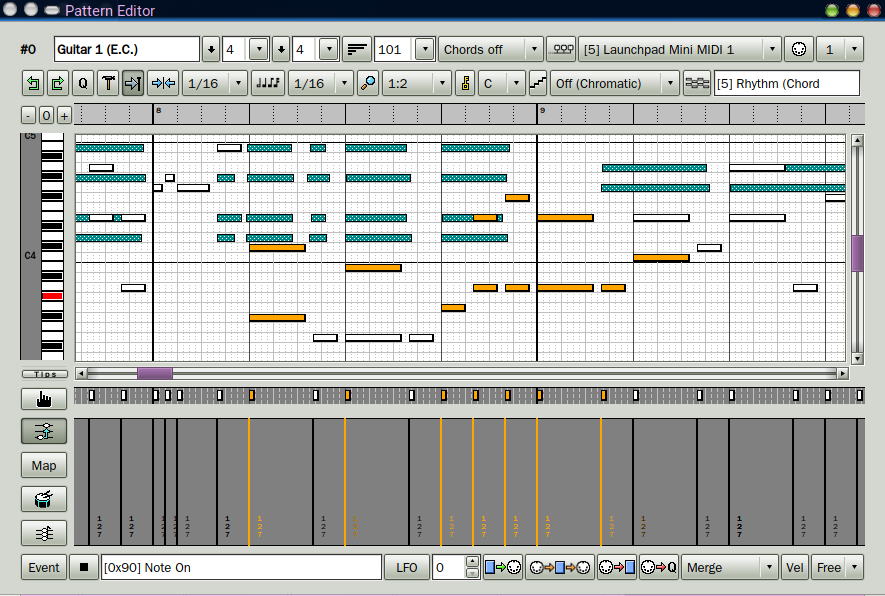
\includegraphics[scale=1.00]{pattern-editor/pattern-edit-window.png}
   \caption{External Pattern Editor Window}
   \label{fig:pattern_editor_window}
\end{figure}

   This figure does not show a recent new feature: for selected event,
   the orange data line is topped with a circular "grab handle" that can
   be used to change the amplitude of the data (e.g. velocity) being
   shown.
  
   The \textbf{Pattern Editor} is complex, and we will discuss the external
   window only since its features are a superset of the \textbf{Edit} tab.
   For exposition, we break the window into the following sections:

   \begin{enumber}
      \item \textbf{First Row}
      \item \textbf{Second Row}
      \item \textbf{Time}
      \item \textbf{Piano Roll}
      \item \textbf{Events Pane}
      \item \textbf{Left Buttons}
      \item \textbf{Data Pane}
      \item \textbf{Bottom Row}
      \item \textbf{Common Actions}
   \end{enumber}

   Before we describe this window, there are some things to recognize.
   First, if the pattern is empty when play is started, the progress bar will
   still move, so that the user can play a MIDI instrument and record new notes.
   Second, to add a note with the mouse the following options turn on painting
   note:

   \begin{itemize}
      \item One must press \textsl{and hold} the \textsl{right}
         mouse button (the pointer changes to a pointing finger),
         press the left mouse button.
      \item Click in the pattern editor, press the
         \index{keys!i}
         \index{keys!p}
         \texttt{p} key to select the "pencil" or "paint" mode,
         or
         \texttt{i} key to select "insert" mode (a la vi),
      \item Click on the "pointing finger" button.
      \item 
   \end{itemize}

   \index{mouse!left-click}
   Left-click to add a note or
   \index{mouse!left-click-drag}
   left-click-drag to add multiple notes as the mouse moves.

   To exit the painting mode,
   \index{keys!x}
   \index{keys!Esc}
   press or release the right mouse button, press
   \texttt{x} to "eXit" or "eXscape" from paint mode,
   or click the "pointing finger" button again.
   \texttt{Esc} also exits paint mode if the pattern is not playing.

   Notes are drawn only with the length selected by the "notes" button
   near the top of the pattern window.  There are tricks to
   modifying the new notes, described later.

   \textsl{Seq66} automatically scrolls
   horizontally through the sequence/pattern editor window when
   playback moves the progress bar past the current frame of data.
   This feature makes it easier to follow patterns that are longer than a
   measure or two.
   One might want to print out the following figure to follow along.  There is
   a lot of functionality in this window.
   Also, some items have changed slightly from when this diagram was made.

\begin{figure}[H]
   \centering 
   \includegraphics[scale=0.90]{pattern-editor/pattern-edit-window-annotated.png}
   \caption{Pattern Editor Window, Annotated}
   \label{fig:pattern_editor_window_annotated}
\end{figure}

   The arrow keys can be used to move left, right, up, or down.
   \index{keys!vi}
   \index{keys!hjkl}
   For \textsl{vi} users, the \texttt{h} (left), \texttt{j} (down),
   \texttt{k} (up), and \texttt{l} (right)
   keys can be used while any pane is in focus, and they act like the arrow
   keys.
   The \texttt{Home} and \texttt{End} keys move to the beginning and end of the
   pattern.
   One can page vertically in the piano roll using the
   \index{keys!page-up} \texttt{Page Up} and 
   \index{keys!page-down} \texttt{Page Down} keys.

\subsection{Pattern Editor / First Row}
\label{subsec:pattern_editor_first_row}

   The top bar (horizontal panel) of the Pattern (sequence) editor
   lets one change the name of
   the pattern/loop/sequence/track, the time signature of the piece, how long
   the track is, and some other configuration items.

   \begin{enumber}
      \item \textbf{Track Number}
      \item \textbf{Track Name}
      \item \textbf{Add Time Signature Event} (not pictured)
      \item \textbf{Beats Per Bar Reset} and \textbf{Beats Per Bar}
      \item \textbf{Beat Width Reset} and \textbf{Beat Width}
      \item \textbf{Pattern Length Reset} and \textbf{Pattern Length}
      \item \textbf{Chord Types}
      \item \textbf{Buss Reset} and \textbf{Buss Selection}
      \item \textbf{Channel Reset} and \textbf{Channel Selection}
   \end{enumber}

   \setcounter{ItemCounter}{0}      % Reset the ItemCounter for this list.

   \itempar{Track Number}{pattern editor!number}
   This item shows the sequence/track/pattern/loop
   number, to make it easier to pick it out when a lot of patterns are being
   edited at once.

   \itempar{Track Name}{pattern editor!name}
   Provides the name of the pattern.
   This name should be short and memorable.
   It is displayed in the \textbf{Live Grid} (the \textbf{Patterns Dialog}),
   on the top line of its pattern slot.

   \itempar{Add Time Signature Event}{pattern editor!time signature}
   This button is shown in the composite picture in
   \sectionref{subsec:pattern_editor_measures_ruler},
   to the left of the beat selector.
   When either the beats/bar or beat width values (see below) are changed,
   and the progress marker is at time 0, then the change is
   saved as a Time Signature Meta event at time 0. Additional changes there
   overwrite that event.
   Otherwise, move the "L" marker and click this button to log another
   time-signature.
   There are interactions between the beats/bar, beat-width, and the length (in
   measures) of the pattern.
   Generally, if both the beats/bar and beat-width are to be changed,
   it is better to change the beat-width first.
   In any case, the measures might have to be adjusted as well.
   It is better to get all the time signatures in place before adding notes.
   To add time signatures at later times in the tune, this must be done:

   \begin{enumber}
      \item Move the mouse cursor to the \textsl{top half} of the time pane;
         the cursor will change to a vertical arrow. Click at the desired time
         and observe the red progress line and "L" marker.
      \item Change the beats-per-measure, if desired.
      \item Change the beats-width, if desired.
      \item Click the \textbf{Add Time Signature} button to log the
         new time signature.
   \end{enumber}

   It adds a time-signature Meta event and adjusts the pattern
   length (if needed) at once.
   The new time signature should appear in the data and event panes as well.

   \itempar{Beats Per Bar}{pattern editor!beats/bar}
   \index{beats per bar}
   Specifies the number of beat units per bar in the time signature.
   The possible values range from 1 to 16, if the drop-down menu is used.
   Arbitrary values up to 32 can be entered by typing the number.
   The "Reset" button resets the value to 4.

   \itempar{Beat Width}{pattern editor!beat width}
   \index{beat width}
   Specifies the size of the bottom beat unit of the time signature:
   1 for whole notes; 2 for half notes; 4 for quarter notes; 8 for eight notes;
   16 for sixteenth notes; and 32 for thirty-second notes.
   The whole time signature is display at the bottom center of the
   corresponding pattern slot in the \textbf{Live Grid}.
   Arbitrary values up to 32 can be entered by typing the number.
   The "Reset" button resets the value to 4.

   Editing a non-power-of-2 beat width yields a warning prompt appears because MIDI tracks can store only time
   signatures where the beat width is a power of 2.
   If the prompt is OK'ed, then the non-standard beat-width is set,
   but it is \textsl{not added as a time-signature event}.
   Instead, it is stored as a SeqSpec event for \textsl{Seq66}.
   Also note that it is difficult to display these time-signatures
   correctly, since the pulse/beat calculations yield non-integers that are
   not detected in displaying a gird.

   \itempar{Pattern Length}{pattern editor!length}
   Sets the length of the current pattern, in measures.
   The possible values range from 1 to 64.
   Arbitrary values up to 1024 can be entered by typing the number.
   \textsl{However}, when opening or importing a non-\textsl{Seq66}
   MIDI tune, the length of each track will be used, and so other values
   are possible.

   Bringing up a pattern less than one measure or bar in
   length in the pattern editor will adjust the pattern to pad it to the
   length of one measure.
   \index{pattern editor!progress bar}
   \textsl{Seq66} will, when it reads such a short pattern
   from a MIDI file,

   \index{expand}
   \index{recording!expand}
   A feature from user \textsl{stazed} allows the pattern to expand
   indefinitely while the user inputs MIDI from a controller, via the
   \textbf{Expand} option of the \textbf{Loop Record Type}.
   This works in \textbf{Live} mode or \textbf{Song} mode.
   The pattern extends continually with or without note entry.
   Once playback starts, the progress bar moves forward.
   Notes are recorded they are played on a MIDI controller.
   Once the end of the measure is neared, another
   measure is added, whether or not more notes are struck.
   The measure-count at the top of the editor shows the current number
   of measures.
   Once playback (and recording) stops, the user can either accept the
   final length, or change the length to a lesser number.
   If the lesser length will drop notes, a prompt will appear
   for the user to accept or reject the length change.

   \itempar{Chord Types}{pattern editor!chord types}
   \index{chord generation}
   This setting allows one to select a chord type (e.g. "major" or "minor").
   When active, a note is treated like the base note of the selected chord
   type, and extra notes are generated to create that chord.
   The \textbf{Chord Generation Reset} button is at the left of the
   \textbf{Data Pane}.
   One can insert chords with one click.
   (This feature comes from user "stazed"
   and his \textsl{Seq32} project \cite{seq32}.)
   Select the desired chord type first.
   Once a value other than \textbf{Off} is selected,
   drawing mode will add multiple notes representing the chord
   created, with the clicked note value as the base of the chord.

   \itempar{MIDI Out Device (Buss)}{pattern editor!midi out device}
   This setting specifies a virtual MIDI output buss or a
   MIDI output device set up by the computer and
   attached MIDI equipment.
   The button resets it to buss 0.
   Note that, if the pattern's selected buss is not found, this entry will be
   blank.  The user must select a valid buss from this dropdown.

   \itempar{MIDI Out Channel}{pattern editor!midi out channel}
   The drop-down selects the MIDI output channel.
   The possible values range from 1 to 16, plus \textsl{Free}, which means
   that the channels of the events are preserved, and are used as the output
   channel, a bit like an SMF 0 track.
   The editing channel is always channel 1; the selected channel is applied
   on playback.
   If instruments are assigned in the 'usr' configuration file
   for that device and channel, their names will be shown in the dropdown.

   In addition, this setting determines the channel applied when painting notes
   in the piano roll.  If set to "1" or "Free" (no channel), then channel 1 is
   applied.  Otherwise, if set to "2" through "16", that channel is applied.

\subsection{Pattern Editor / Second Row}
\label{subsec:pattern_editor_second_row}

   The second horizontal panel of the Pattern Editor provides a number
   of additional settings and functions:

   \begin{enumber}
      \item \textbf{Undo}
      \item \textbf{Redo}
      \item \textbf{Quantize Selection}
      \item \textbf{Tools Popup}
      \item \textbf{Follow Progress}
      \item \textbf{Reset Snap} and \textbf{Grid Snap}
      \item \textbf{Note Length Reset} and \textbf{Note Length}
      \item \textbf{Zoom Reset} and \textbf{Zoom}
      \item \textbf{Key Reset} and \textbf{Key of Sequence}
      \item \textbf{Scale Reset} and \textbf{Musical Scale}
      \item \textbf{Background Sequence}
   \end{enumber}

%  \setcounter{ItemCounter}{0}      % Reset the ItemCounter for this list.

\subsubsection{Pattern Editor / Undo/Redo}
\label{subsubsec:pattern_editor_second_row_undo_redo}

   \setcounter{ItemCounter}{0}      % Reset the ItemCounter for this list.

   \itempar{Undo}{pattern editor!undo}
   The \textbf{Undo} button rolls back any changes to the pattern from this
   session.  It will roll back one change each time pressed.
   \index{keys!ctrl-z}
   Pressing \texttt{Ctrl-Z} is the same as using the \textbf{Undo} button.

   \itempar{Redo}{pattern editor!redo}
   The \textbf{Redo} button will restore any undone changes to the pattern from
   this session.
   It will restore one change each time it is pressed.
   There is currently no redo key.

\subsubsection{Pattern Editor /  Quantize Selection}
\label{subsubsec:pattern_editor_second_row_quantize_selection}

   \index{quantize}
   \index{pattern editor!quantize}
   This button quantizes the selected events as per
   the \textbf{Grid Snap} setting.

\subsubsection{Pattern Editor / Tools Popup}
\label{subsubsec:pattern_editor_second_row_tools_popup}

   This button brings up a nested menu of tools for modifying selected
   events and notes.

   \begin{enumber}
      \item \textbf{Select Notes...}.
      Selects Note Ons, Note Offs, and Aftertouch.
      In order for notes to be modified by quantization or randomization,
      they need to be selected first, otherwise some menu entries are
      disabled.
      Notes can be selected in the piano roll of via this menu.
      This menu provides two note-selection options:
         \begin{itemize}
            \item \textbf{Select all}. Selects all notes in the pattern;
               \index{keys!ctrl-a} \texttt{Ctrl-A} will also select
               all of the events in the pattern editor.
            \item \textbf{Invert selection}. Inverts the selection of notes.
         \end{itemize}
      \item \textbf{Note timing/velocity...}. This menu
            offers four ways to tweak the timing of the selected notes:
         \begin{itemize}
            \item \textbf{Quantize}.
               \index{quantize}
               Quantizes the selected notes in time, the same way as the
               \textbf{Quantize} ("\textbf{Q}") button.
            \item \textbf{Tighten}.
               \index{tighten}
               This operation merely a less strict form of quantization.
            \item \textbf{Jitter}.
               \index{jitter}
               Jittering modifies the timing of a note by adding or subtracting
               a small random of time.
            \item \textbf{Randomize velocity}.
               \index{randomize}
               This operation modifies the velocity of a note by a small
               amount.
         \end{itemize}
      \item \textbf{Pitch transpose}. Allows uniform transpostion
         regardless of the key and scale in force for the pattern.
         \index{modify pitch}
         Selecting this item entry brings up a sub-menu.
      \item \textbf{Harmonic transpose}. Makes sure
         that all transpositions stay on the selected scale.
         If the scale selection is \textbf{Off}, this is the same as plain
         pitch transpose, and so is not enabled.
      \item \textbf{LFO}. Allows for modulating of control values with a
         low-frequency oscillator.
         See \sectionref{subsec:pattern_editor_bottom}.
      \item \textbf{Pattern fix}. Allows for fixing up a new pattern
         that was recorded with some timing errors, or transforming the
         pattern in various ways.
      The pattern fix dialog provides a way for more control over the
      modifications of a pattern.
      It's complex and deserves a section of its own.
      See \sectionref{subsec:pattern_editor_pattern_fix}.
   \end{enumber}

\subsubsection{Pattern Editor / Follow Progress}
\label{subsubsec:pattern_editor_second_row_follow_progress}

   \index{follow progress}
   This button toggles whether or not the progress bar follows
   progress in long patterns.  Turning off this feature is useful when
   one wants to concentrate on the current measure without the paging to
   subsequent measures that occurs with the "follow progess" feature.

\subsubsection{Pattern Editor / Snap Reset and Grid Snap}
\label{subsubsec:pattern_editor_second_row_grid_snap}

   \index{grid snap}
   \index{pattern editor!grid snap}
   Grid snap selects where the notes will snap when
   \textsl{drawn} and when \textsl{moved} (but not when lengthened/shortenend).
   That is, it selects the snap-spacing for the notes.
   It also applies to moving selected notes horizontally with the
   arrow keys.

   The following values are supported:
   \textbf{1}, \textbf{1/2}, \textbf{1/4}, \textbf{1/8},
   \textbf{1/16} (\textsl{the default value}),
   \textbf{1/32}, \textbf{1/64}, and \textbf{1/128}.
   Additional values are also supported:
   \textbf{1/3}, \textbf{1/6}, \textbf{1/12}, \textbf{1/24},
   \textbf{1/48}, \textbf{1/96}, and \textbf{1/192}.
   The button to the left of this control resets it to the default value.

\subsubsection{Pattern Editor / Note Length Reset/Note Length}
\label{subsubsec:pattern_editor_second_row_note_length}

   \index{note length}
   \index{pattern editor!note length}
   Note length determines the duration of inserted (drawn by the mouse)notes.
   Like the \textbf{Grid Snap} values,
   the following values are supported:
   \textbf{1}, \textbf{1/2}, \textbf{1/4}, \textbf{1/8},
   \textbf{1/16} (\textsl{the default value}),
   \textbf{1/32}, \textbf{1/64}, and \textbf{1/128}.
   Additional values are also supported:
   \textbf{1/3}, \textbf{1/6}, \textbf{1/12}, \textbf{1/24},
   \textbf{1/48}, \textbf{1/96}, and \textbf{1/192}.
   The button to the left of this control resets it to the default value.

\subsubsection{Pattern Editor / Zoom Reset/Zoom}
\label{subsubsec:pattern_editor_second_row_zoom_reset}

   \index{zoom!horizontal}
   \index{pattern editor!horizontal zoom}
   Horizontal zoom is the ratio between MIDI pixels and ticks, written as
   "pixels:ticks", where "ticks" is the "pulses" in "PPQN".
   For example, 1:4 = 4 ticks per pixel.
   Supported values are
   \textbf{1:1}, \textbf{1:2} (\textsl{the default value}),
   \textbf{1:4}, \textbf{1:8}, \textbf{1:16},
   and \textbf{1:32}, along with
   more values to support higher PPQN tunes:
   \textbf{1:64}, \textbf{1:128}, \textbf{1:256}, and \textbf{1:512}.
   The default zoom is 2 for the standard PPQN value, 192, but it
   increases for higher PPQN values, so that the default zoom looks sensible.
   As the right number (ticks) goes higher,
   the effect is to zoom out, and show more of the pattern.
   The button to the left of this control resets it to the default value.
   Zoom can also be changed via the \texttt{Z} and \texttt{Z} keys, and
   reset by the \texttt{0}.

\subsubsection{Pattern Editor / Key Reset/Key}
\label{subsubsec:pattern_editor_second_row_musical_key}

   \index{key}{pattern editor!key}
   Selects the desired musical key for the pattern.  The following keys are
   supported:
   \textbf{C}, \textbf{C\#},
   \textbf{D}, \textbf{D\#},
   \textbf{E}, \textbf{F}, \textbf{F\#},
   \textbf{G}, \textbf{G\#},
   \textbf{A}, \textbf{A\#},
   and \textbf{B}.
   Changing the key shifts the marked note-rows
   for the \textbf{Musical Scale} setting and indicates the base notes
   of the key in a \textbf{bold} font.
   The small key button resets the key to \textbf{C}.

   \index{save musical key}
   The musical key that a sequence/pattern is set to is
   saved in the MIDI file along with the rest of the data for the sequence.
   \textbf{However},
   a change made to the key, scale,
   or background sequence (not to be confused with background-recording)
   in the pattern editor can be saved in the whole song,
   so that opening another sequence
   will apply the same settings to that sequence.  This is an optional feature,
   supported as noted below.
   Also see \textbf{Musical Scale} below for the scale-identification feature.

   \index{global-sequence}
   If the global-sequence feature is enabled, and the user selects
   a different key, scale, or background sequence in the pattern editor, 
   then \textsl{all} patterns share the selected key, scale, or background
   sequence.  Furthermore, these settings are saved in the "proprietary"
   section of the MIDI file, where they are available for all patterns.

   If the global-sequence feature is \textsl{not} enabled, and the user selects
   a different key, scale, or background sequence in the pattern editor, 
   then only that pattern will use the selected key, scale, or background.
   The key, scale, or background sequence change will be saved in the MIDI file
   only for that pattern, as a SeqSpec meta event.
   The global-sequence feature setting can be made in the 'usr' configuration
   file.

\subsubsection{Pattern Editor / Scale Reset/Musical Scale}
\label{subsubsec:pattern_editor_second_row_musical_scale}

   \index{scale}
   \index{pattern editor!musical scale}
   Selects the desired background scale for the pattern; it provides a way for
   someone to key in notes that are only in that scale.
   When a scale is selected, the following features are supported:

   \begin{itemize}
      \item The note grid lines that are \textsl{not}
         in the scale are painted grey in the piano roll.
      \item For harmonic transposition, the notes are shifted
         so that they remain in the selected scale.
      \item The exact notes that are considered "in-scale" shift according
         to the value of the selected \textbf{Key of Sequence}.
   \end{itemize}

   \index{musical scales}
   The following musical scales are supported so far:

   \begin{itemize}
      \item \textbf{Off (Chromatic)}
      \item \textbf{Major (Ionian)}
      \item \textbf{Minor (Aeolian)}
      \item \textbf{Harmonic Minor}
      \item \textbf{Melodic Minor}
      \item \textbf{Whole Tone}
      \item \textbf{Blues}
      \item \textbf{Major Pentatonic}
      \item \textbf{Minor Pentatonic}
      \item \textbf{Phrygian}
      \item \textbf{Enigmatic}
      \item \textbf{Diminished}
      \item \textbf{Dorian}
      \item \textbf{Mixolydian}
   \end{itemize}

   Please let us know of any mistakes in these scales.
   Note that the \textbf{Melodic Minor} scale is supposed to
   descend in the same way as the natural \textbf{Minor} scale, but
   there is no way to support that trick in \textsl{Seq66}.

   One can select which \textbf{Musical Scale} and
   \textbf{Key} the piece is in nominally,
   and \textsl{Seq66} will grey those keys on the piano-roll that
   are \textsl{not} in the selected scale for the selected key.
   This is purely visual; a user can still add off-key notes.
   This feature makes it easier to stay in key while playing and recording.
   The scale will shift when a different \textbf{Key} is selected.

   \index{save musical scale}
   The scale that a pattern is set to is
   saved in the MIDI file along with the rest of the data for the pattern.
   A change made to the key, scale, or background pattern in
   the pattern editor can be saved globally, so that opening another pattern
   apply the same settings to that pattern.  This is a configurable feature in
   the 'usr' file; see "global-seq-feature".
   This option allows applying the key/scale/background-sequence
   either globally (all patterns) or locally (per-pattern), with each pattern
   holding its key, scale, and background-sequence settings in
   SeqSpec meta events.

   \index{scale identifier}
   \index{keys!ctrl-k}
   The pattern editor's piano roll has a little secret:
   the \textbf{Scale Identifier}.
   When the piano roll has focus and \texttt{Ctrl-K} is pressed,
   all of the notes in the pattern are analyzed to try to determine
   the both the key and the scale of the existing notes.
   The method is not sophisticated... the notes are counted and are matched
   against all of the keys (C to B) and scales supported by \textsl{Seq66}.
   The combinations with the highest number of notes are then shown in a
   message box.
   This simple analysis depends on having at least 8 notes in the pattern, and
   it is possible to get weird results if
   there are only a few \textsl{different}
   notes, as in a simple bass line.
   Don't expect miracles from this feature.
   A more sophisticated analysis, the
   \textsl{Krumhansl-Schmuckler} key-finding
   algorithm, could be used, but it is a bit too complex
   for our needs, which are basic.

\subsubsection{Pattern Editor / Background Sequence}
\label{subsubsec:pattern_editor_second_row_background_sequence}

   \index{background sequence}
   \index{pattern editor!background sequence}
   One can select another pattern to draw on the background to help with
   writing corresponding parts.
   The button brings up a small menu with values of \textbf{Off} and
   \textbf{Set 0} (at a minimum).
   The 0 is a set number; sets are numbered from 0 to 31.
   Additional set numbers appear in the menu for each set that has data in it.
   Under the \textbf{Set 0} entry, a menu appears.
   Once the desired pattern is selected from that list, it appears as dark cyan
   note bars, along with the normal notes that are part of the pattern.

   \index{save background sequence}
   The background sequence that shows is saved in the MIDI file
   along with the rest of the data for the sequence/pattern.
   A change made to the key, scale, or background sequence in
   the pattern editor is saved in the editor, so that opening another sequence
   will apply the same settings to that sequence.
   This is an optional feature, as noted earlier.

\subsection{Pattern Editor / Measures Ruler}
\label{subsec:pattern_editor_measures_ruler}

   The measures ruler ("bar indicator", or "Time")
   consists of a \textsl{timeline} at the top and the 
   \textbf{L marker} and \textbf{R marker} items.
   The following are the elements next to and on
   the \textbf{Time} line.

\subsubsection{Pattern Editor / Measures Ruler / Vertical Zoom}
\label{subsubsec:pattern_editor_measures_ruler_vertical_zoom}

   \index{vertical zoom}
   \index{pattern editor!vertical zoom}
   The vertical zoom buttons
   allow the user to compress, reset, or expand the
   piano roll vertically.
   The \texttt{v}, \texttt{V}, and \texttt{0} keys offer
   the same functions.

   A more permanent change in vertical grid scaling
   can be made by setting the \textbf{Editor Key Height} value in
   the \textbf{Edit / Preferences / Display} tab,
   or in the 'usr' file.

\subsubsection{Pattern Editor / Measures Ruler / Time Bar}
\label{subsubsec:pattern_editor_measures_ruler_time_bar}

      The \textbf{Time} (or \textbf{Measures}) bar provides an explicit
      count of beats and bars.
      It follows the horizontal zoom of the piano roll.
      It also has a couple tricks, which are shown in the diagram below.

      \begin{itemize}
         \item \textbf{In the upper half} of the time-line,
            the mouse pointer changes to a vertical pointer.
            Clicking there then shows a vertical bar and a red dot; these mark
            the starting position of playback.
            This is useful for reviewing some notes.
         \item \textbf{In the lower half} of the time-line,
            the mouse pointer changes to a "finger" icon.
            Left-clicking there then moves the "L" marker to that point.
            Right-clicking there moves the "R" marker to that point.
            ("R" will never precede "L", though).
            If the \textbf{Loop} button in the main window is active, then
            playback will loop between the "L" and "R" buttons.
            This looping now works with both Live and Song modes.
      \end{itemize}

   The following figure shows three steps in cursor movement, and the final
   result for setting a time-signature.

\begin{figure}[H]
   \centering 
   \includegraphics[scale=0.65]{pattern-editor/seqtime-cursor-composite.png}
   \caption{Setting a Time Signature}
   \label{fig:pattern_editor_seqtime_cursor_composite}
\end{figure}

   The steps shown are

   \begin{enumber}
      \item The mouse cursor is in the piano roll, and has the normal
         appearance for the current mouse cursor theme.
      \item The mouse cursor is in the bottom half of the time line, and
         here it's a pointing finger.
         When left-clicked, the "L" marker is set there.
         When right-clicked, the "R" marker is set there.
      \item The mouse cursor is in the top half of the time line, and is
         shown as a vertical arrow.
         A left- or right-click sets the current position in the
         pattern, and a red vertical line marks that position.
      \item The time-signature button (the "4/8" shown in the top
         bar) is clicked, and a time-signature is added at that point.
      \item The data pane switches to show Time Signatures.
         These cannot be edited in the data pane, but in the event bar above
         it, they can be selected by drawing a box around them, and then
         be either deleted or moved with the Left/Right arrow keys.
   \end{enumber}

   Note that the "L" and "R" markers can be selected via the keyboard using
   their respective shifted key.  Once selected, the marker can be moved left
   or right using the left and right arrow keys.
   Also note that the default position of the "R" marker is at the end of the
   fourth measure, so it might not be visible in the pattern editor without
   scrolling to it.

\subsection{Pattern Editor / Piano Roll}
\label{subsec:pattern_editor_piano_roll}

   The piano roll is the center of the pattern/loop/track/sequence editor.
   When a pattern is opened in the editor, the piano roll scrolls
   automatically to the first notes.

   The piano roll is accompanied by a thin "event bar"
   ("event pane") just below it,
   and a taller "data pane" or "data area" just below that.
   While the pattern editor is very similar to note editors in other
   sequencers, it is a bit different in feel.  A good mouse with at least 3
   buttons is very helpful for editing.  Buttons and keystrokes enhance the
   ease of editing.

   The piano roll shows notes, and, optionally, a background pattern or a
   scale.  Notes are shown as narrow rectanges; the background
   pattern and scale are shown as bars running the length of the piano roll.

   When the piano roll has keyboard focus, the \texttt{Space} key
   starts and stops playback, rewinding to the beginning when stopped.
   The \texttt{.} (period) key starts and pauses playback, without
   rewinding.
   The first \texttt{Esc} key stops playback;
   the second \texttt{Esc} key exits "paint" mode; and
   the third \texttt{Esc} key closes the pattern editor \textsl{if}
   the 'usr' \texttt{[pattern-editor] escape-pattern} option is set.
   This functionality is similar to that of the main window, but
   these keys are not reconfigurable in the piano roll.

   One can page vertically in the piano roll using the
   \index{keys!page-up} \texttt{Page Up} and 
   \index{keys!page-down} \texttt{Page Down} keys.
   One can go to the leftmost position using the 
   \index{keys!ctrl-home} \texttt{Home} key,
   and to the rightmost position using the
   \index{keys!ctrl-end} \texttt{End} key,
   The mouse scroll wheel can also be used to move the panes around.
   For implementation reasons, the scroll wheel is active
   \textsl{only} in the piano roll.

   \index{keys!arrows}
   \textsl{If no notes are selected}, the arrow keys will move the piano row
   up, down, left, and right in small steps.
   Otherwise, the selected notes are moved
   up, down, left, and right.

   \index{keys!hjkl}
   In addition, the "vi" keys \texttt{h}, \texttt{j}, \texttt{k}, and
   \texttt{l} will act like the arrow keys. This can be convenient, especially
   if the arrow-keys are unwieldly.  For example, the
   \textsl{Microsoft Arc} keyboard puts all four arrows on one button!

   \index{keys!ctrl-arrows}
   \textsl{If no notes are selected}, then \texttt{Ctrl-Left-Arrow}
   and \texttt{Ctrl-Right-Arrow} will move the progress bar to the left or
   right by one snap value.

   \index{step}
   \index{note step}
   With the note-step feature, if one paints notes with the mouse,
   the note position advances with each click.
   If one paints notes via an external MIDI keyboard, the notes are painted and
   the note position advances.
   To preview notes entered via a MIDI device, click the
   \textbf{MIDI Thru} button to activate so that they will be
   passed to the sound generator or software synthesizer.

\subsubsection{Pattern Editor / Piano Roll Items}
\label{subsubsec:pattern_editor_piano_roll_items}

   The center of the pattern editor consists of a time panel at the top,
   a virtual keyboard at the left, a note grid, a vertical scrollbar, an event
   panel, and a data panel at the bottom.

   \begin{enumber}
      \item \textbf{Beat}
      \item \textbf{Measure}
      \item \textbf{Virtual Piano Keyboard}
      \item \textbf{Notes}
   \end{enumber}

   \setcounter{ItemCounter}{0}      % Reset the ItemCounter for this list.

   \itempar{Beat}{piano roll!beat}
   The light vertical lines represent the beats defined by the configuration
   for the pattern.  The even lighter dotted lines between the beats are useful
   for snapping notes.

   \itempar{Measure}{piano roll!measure}
   The heavy vertical lines represent the measures (bars) defined by the
   configuration for the pattern.
   \index{pattern!end marker}
   Also note that the end of the pattern
   occurs at the end of a measure, and is marked by a blocky \textbf{END}
   marker.

   \itempar{Virtual Piano Keyboard}{piano roll!virtual piano keyboard}
   The virtual keyboard is a fairly powerful interface.  It shows,
   by shadowing, which note on the keyboard will be drawn. It can be
   played with a mouse, using left-clicks, to preview a short motif.
   Every octave, a note letter and octave number are shown, as in
   "C4".  If there is a difference scale in force, then the letter changes to
   match, as in "F\#5".

   \index{virtual keyboard!right-click}
   A right-click in the virtual keyboard area toggles the display
   between octave-note letters, MIDI note-numbers, and other views.
   The following figure shows all views, superimposed for comparison.

\begin{figure}[H]
   \centering 
   \includegraphics[scale=1.00]{pattern-editor/pattern-edit-window-key-numbers.png}
   \caption{Virtual Keyboard Number and Note Views}
   \label{fig:pattern_editor_key_numbers}
\end{figure}

   \itempar{Notes}{piano roll!notes}
   Musical notes are indicated in the piano roll
   by thick horizontal bars with white
   centers.  Each bar provides
   a visual representation of the pitch of a note and the length of a note.
   The current scale and background pattern can also be shown in the piano
   roll.

   \itempar{Time Scroll}{pattern editor!time scroll}
   Allows one to pan through the whole pattern, if it is too long to fit in
   the window horizontally.

\subsubsection{Pattern Editor / Note Painting}
\label{subsubsec:pattern_editor_note_painting}

   When we say "editing" in the context of the piano roll, in part we mean that
   we will "draw"
   \index{draw mode}
   \index{mode!draw}
   \index{paint mode}
   \index{mode!paint}
   or "paint" notes.
   Drawing, modifying, copying, and deleting notes is fairly easy in
   \textsl{Seq66}, though slightly different from other MIDI sequencers.

   The \textsl{Seq24} note-editing style is as expected for basic
   actions such as selecting and moving notes using the left mouse button.
   Drawing a note or event is a bit different, in that one must first
   enter the drawing mode ("paint mode").
   One way is to \textsl{click and hold} the right mouse button, and then
   \textsl{click and drag} the mouse to insert notes.
   (Note that one can use the \textsl{Ctrl-left-click} as a middle click. )
   \index{keys!p}
   Another way is to use the \texttt{p} key to enter the "paint" mode.
   To get out of the "paint" mode, press the
   \index{keys!x}
   \index{keys!Esc}
   \texttt{x} key while in the sequence editor.
   The \texttt{Esc} key also exits paint mode if the tune is not playing.
   Also available is a "finger" button
   (\textbf{Note Select/Note Entry})
   to click to toggle the mode.

   \index{notes!inserting}
   Notes are inserted to be at the current length and grid-snap values for
   the sequence editor for as long as the buttons are pressed while the mouse
   is dragged.
   The length of the note will
   be that specified in the note-length setting (e.g. "1/16").
   \index{auto-note}
   This is the "auto-note" feature.
   The auto-note feature also works with chord-generation.
   Notes are inserted only up to the specified sequence length.
   Once notes are inserted, moving the mouse with the left button still
   held down moves the notes to the new note value of the mouse.
   If one releases the left button, then presses and holds it again,
   more notes will be added in the same way.
   This is a good way to layer notes in a short sequence.
   The draw mode has the following features:

   \begin{itemize}
      \item Notes are continually added as the mouse is dragged ("auto-notes").
      \item Notes cannot be added past the "END" marker of the pattern, which
         marks the \textbf{Sequence Length in bars} setting.
      \item As the mouse is dragged while the left button is held in draw mode,
         notes are either added, or, if already present at that note-on time,
         are moved up and down.
      \item If the draw mode is exited, and entered again, then the original
         notes will not be altered.  Instead, new ones will be added.
      \item Notes can be added while the pattern is playing, and will be heard
         the next time the progress bar passes over them.
   \end{itemize}

   Drawing/painting can also be done while the sequence is playing,
   and notes will be added to be played the next time the progress bar crosses
   them.

\subsubsection{Pattern Editor / Note Editing}
\label{subsubsec:pattern_editor_note_editing}

   Once notes are in place, whether by recording or using "paint" mode,
   the piano roll provides a sophisticated set of note-editing
   actions.
   But, before editing, one can turn on
   \index{note!tooltips}
   "note tooltips", if desired.
   The thin button, labelled in tiny text as "Note Tips"
   next to the horizontal scroll bar toggles this mode.
   When enabled, moving the mouse over a note will show its value, time range
   in units of B:B:T, and its velocity.
   This view is quicker than opening up the \textbf{Event Editor}.
   Onward!

   \setcounter{ItemCounter}{0}      % Reset the ItemCounter for this list.

   \itempar{Event Selection}{event!select}
   There are various ways to select events and copy, delete, or modify them
   using the mouse or the keyboard in the piano roll:

   \begin{itemize}
      \item
         \index{keys!ctrl-a}
         \index{selection!all}
         \textbf{\texttt{Ctrl-A}}.
         Pressing the \texttt{Ctrl-A} key will select all of the events in the
         pattern editor.
      \item
         \index{keys!ctrl-e}
         \index{selection!events by channel}
         \textbf{\texttt{Ctrl-E}}.
         Pressing the \texttt{Ctrl-E} key will select all of the events in the
         pattern editor that have the channel that is selected in the
         channel dropdown.
         This selection is useful if one wants to move events from one channel
         into another pattern.
      \item
         \index{keys!ctrl-n}
         \index{selection!notes by channel}
         \textbf{\texttt{Ctrl-N}}.
         Pressing the \texttt{Ctrl-N} key will select all of the notes
         in the pattern editor that have the channel that is selected in the
         channel dropdown.
         This selection is useful if one wants to move notes from one channel
         into another pattern.
      \item
         \index{mouse!left-click}
         \index{pattern editor!left click}
         \index{pattern editor!select note}
         \textbf{Left Click}.
         Pressing the left button on a note or a event deselects all other
         notes or events, and selects the item clicked on.
         The selected note will turn orange (or the configured palette color).
      \item
         \index{mouse!left-click-drag}
         \index{pattern editor!select multiple notes}
         \textbf{Left Click Drag}.
         Pressing the left mouse button and dragging also lets one
         select ("lasso") multiple events and notes.
         The selected notes will turn orange.
         Adjustments can be made to one or more notes by selecting one or more
         notes, and then applying one or more special
         \index{selection action}
         "selection actions" to the selection.
         Be careful!  If you \texttt{Ctrl-left-click-drag}
         on an already-selected note,
         the drag will change the length of
         \textsl{all of the notes in the selection}.
      \item \index{mouse!ctrl-left-click}
         \textbf{Ctrl Left Click}.
         Pressing the \texttt{Ctrl} key and the left button on a note or an
         unselected event \textsl{adds} that event to the selection.
      \item
         \index{pattern editor!transpose notes}
         \textbf{Left Click Drag Selection Up/Down}.
         To move notes in pitch, once selected, grab one of the notes in the
         selection and drag it upward or downward.
         \index{down arrow}
         \index{up arrow}
         Also, when a selection is in force, the
         \texttt{Up} and \texttt{Down} arrow keys will
         change the pitch of every note in the selection.
         The smallest unit of pitch change is one MIDI note value.
      \item
         \index{pattern editor!move notes in time}
         \textbf{Left Click Drag Selection Left/Right}.
         To move notes in time, once selected, grab one of the notes in the
         selection and drag it leftward or rightward.
         \index{left arrow}
         \index{right arrow}
         Also, since a selection is in force, the
         \texttt{Left} and \texttt{Right} arrow keys can also
         be used to change the time of every note in the selection.
         The smallest unit of time change is the \textbf{Grid snap} value,
         which might be a 16th note, for example.
      \item
         \index{mouse!ctrl-left-click-drag}
         \textbf{Ctrl Left Click Drag}.
         \begin{itemize}
            \item Pressing the \texttt{Ctrl} while left-click-dragging
               \textsl{on unselected events} lets one make additional
               selections of multiple events and notes.
            \item Pressing the \texttt{Ctrl} while left-click-dragging
               \textsl{on an already-selected event} lets one stretch or
               compress the lengths of all notes in the selection.
%              Also achievable via a \textbf{Middle Click Drag}.
               \index{pattern editor!event stretch}
               \index{event!stretch}
               \index{pattern editor!event compression}
               \index{event!compression}
               This feature is called \textsl{event stretch}
               or \textsl{event compression}.
               Notes can be shortened below the default note length by event
               compression.  There is currently no way to change the length of
               the note using a keystroke.
         \end{itemize}
      \item \index{pattern editor!deselect notes} \index{selection!deselect}
         \textbf{Deselect Notes}
   \end{itemize}

   \index{note!selection box}
   The selection, copying, and pasting of notes has some minor tricks to
   remember.  When some notes are selected, the effective selection box
   goes from the first note to the last note, and from the top-most note to the
   bottom-most note.
   When pasting the notes, place the mouse cursor so that it lies on the
   desired row for the top-most note, and on the desired time location for the
   left-most note.  After pasting, be sure to verify the notes in the new
   location.

   \index{warning!wrap-around notes}
   \textbf{Warning}:  Reducing or increasing the length of a note selection
   by too much causes the note or notes to "wrap-around" to the end
   of the pattern boundary and grow more from the beginning of the sequence. 
   If it happens, one probably ought to undo it.

   The \textbf{Tools} button described in
   \sectionref{subsec:pattern_editor_second_row} can also be used to
   modify selections.
   Once one or more notes are selected, they can be modified in time,
   pitch, or length, as described above.

   \textbf{Warning:}
   \index{warning!down arrow}
   \index{warning!up arrow}
   \index{warning!note loss}
   If one moves the selection too low or too high in pitch, whether with the
   mouse or the arrow keys, any notes that go below the lowest MIDI pitch or
   above the highest MIDI pitch \textbf{will be lost}!
   If done using the mouse, the undo feature (\texttt{Ctrl-Z}) will work.
   If done using the arrow keys, the undo feature does not work!
   Be careful, especially if you have a fast keyboard repeat rate!

   Note that there is no possibility of note loss with a change in time.  When
   a note disappears at one end of the pattern boundary, it wraps around to the
   other end.  Cool.

   \itempar{Copy/Paste}{pattern editor!copy/paste}
   Copying, cutting, and pasting is supported by selecting a number of events
   or notes, and using the
   \index{pattern editor!cut}
   \index{keys!ctrl-x} Cut (\texttt{Ctrl-X}), 
   \index{pattern editor!copy}
   \index{keys!ctrl-c} Copy (\texttt{Ctrl-C}), and
   \index{pattern editor!paste}
   \index{keys!ctrl-v} Paste (\texttt{Ctrl-V})
   keys.
   When the notes are selected,
   \index{pattern editor!delete}
   \index{keys!del}
   \index{keys!backspace}
   one can delete them with the \texttt{Delete} or \texttt{Backspace} key.
   If the events are \textsl{cut}, using the \texttt{Ctrl-X} key, then
   they can be pasted, using the \texttt{Ctrl-V} key, then
   moving the cursor to the desired place, and clicking.

   One can move the selection box using the arrow keys, to the
   desired location, and then click to
   drop the notes at that location.
   Selected notes that are cut or copied can also be
   pasted into \textsl{other} pattern editor dialogs; that is, they can be
   pasted into other sequences.

\subsubsection{Pattern Editor / Misc Keys}
\label{subsubsec:pattern_editor_misc_keys}

   Here are some other, less standard,` keys useful in the pattern editor piano
   roll:

   \begin{itemize}
      \item
         \index{keys!c}
         \index{selection!repitch}
         \textbf{\texttt{c}}.
         Pressing the \texttt{c} key will attempt to use the note-mapper data
         (provided by a \texttt{*.drums} file) to change the notes in the
         pattern.  This will work only if the pattern is marked as transposable,
         to add some safety against multiple pitch changes; these are useful once
         when converting from one drum machine to General MIDI.
      \item
         \index{keys!ctrl-d}
         \index{selection!clear}
         \textbf{\texttt{Ctrl-D}}.
         Pressing the \texttt{Ctrl-D} key will clear the pattern clipboard.
      \item
         \index{keys!f}
         \index{selection!edge fix}
         \textbf{\texttt{f}}.
         Pressing the \texttt{f} key will attempt to fix wrap-around notes by
         moving the note.
      \item
         \index{keys!ctrl-k}
         \index{selection!analyze}
         \textbf{\texttt{Ctrl-k}}.
         Pressing the \texttt{Ctrl-k} key will analyze all the notes in the
         pattern to try to guess its scale, as discussed earlier.
      \item
         \index{keys!o}
         \index{recording toggle}
         \textbf{\texttt{q}}.
         Pressing the \texttt{o} key will toggle recording for the pattern.
      \item
         \index{keys!q}
         \index{selection!quantize}
         \textbf{\texttt{q}}.
         Pressing the \texttt{q} key will quantize the selected notes.
      \item
         \index{keys!r}
         \index{selection!randomize}
         \textbf{\texttt{r}}.
         Pressing the \texttt{r} key will quantize the selected notes.
      \item
         \index{keys!t}
         \index{selection!tighten}
         \textbf{\texttt{t}}.
         Pressing the \texttt{t} key will partially quantize (tighten)
         the selected notes.
      \item
         \index{keys!u}
         \index{selection!remove unlinked notes}
         \textbf{\texttt{u}}.
         Unlinked notes no longer occur.  But....
%        Unlinked notes do not occur unless note-wrap-around occurs.
%        When they do occur, they are painted in magenta.
         Pressing the \texttt{u} key will remove any unlinked notes found in
         the pattern.
         This fix is a stop-gap until we can figure out
         the best way to prevent unlinked notes while handling recording of
         notes near the end of the pattern length.
      \item
         \index{keys!=}
         \index{selection!relink notes}
         \textbf{\texttt{=}}.
         Pressing the \texttt{=} key relinks any unlinked notes found in
         the pattern. This causes the notes that are unlinked to be linked, and
         thus wrap around.
      \item
         \index{keys!space (play)}
         The default keystroke for starting playback is the \texttt{Space}
         character.
      \item
         \index{keys!esc (stop)}
         The default keystroke for stopping playback is the \texttt{Escape}
         character.
      \item
         \index{keys!period (pause)}
         The default keystroke for pausing playback is the \texttt{Period}
         character.
   \end{itemize}

\subsubsection{Pattern Editor / Zoom Keys}
\label{subsubsec:pattern_editor_zoom_keys}

   \index{zoom keys}
   \index{keys!0}
   \index{keys!z}
   \index{keys!shift-z}
   After a left-click in the piano roll, the
   \textbf{z}, \textbf{Z}, and \textbf{0}
   can be used to zoom the piano-roll view \textsl{horizontally}.
   The \textbf{z} key zooms out (smaller),
   the \textbf{Z} key zooms in (larger),
   and the \textbf{0} key resets the zoom to the default value.
   The horizontal zoom feature also affects the time-line
   (measures indicator) and the data area.

   \index{keys!v}
   \index{keys!shift-v}
   The note display can also be zoomed vertically.
   The \textbf{v} key zooms out vertically to make the notes thinner,
   the \textbf{V} key zooms in vertically to make the notes fatter,
   and the \textbf{0} key resets the zoom to the value of the "key height"
   setting in the 'usr' configuration file.
 
\subsection{Pattern Editor / Events Pane}
\label{subsec:pattern_editor_events_pane}

   The narrow (a few pixels high) events strip shows discrete events,
   such as \texttt{Note On} and \texttt{Note Off}.
   The events that are shown are selectable in the \textbf{Event} category
   selector and the "Selector for Existing Data"" drop-downs at bottom left.
   \index{event strip}
   These and other events appear
   as small squares in the event strip, along with a black vertical bar
   in the \textbf{Data Pane} with a
   height proportional to the data-value of the event and a numeric
   representation of that value.
	The event value (data) editor (directly under the event strip) is used 
	to change note velocities, channel pressure, control codes,
	patch select, etc.

   \textsl{We currently recommend being careful of editing or selecting events
   in that pane (feel free to disobey)}.
   Note On and Note Off events cannot be inserted in the event strip;
   it is too easy to screw up.
   Selection and editing in the events pane is disabled for
   \textbf{Note On}, \textbf{Note Off}, and \textbf{Aftertouch}.
   
   However, when in edit mode (the finger mode), other events, when
   selected in the event menus, can be inserted
   by a click in the event pane.
   Their values can be changed in the data pane.
 
\subsubsection{Pattern Editor / Events Pane / Non-Note Events}
\label{subsubsec:pattern_editor_events_pane_non_note_events}

   \index{events!insert}
   Other event types (including tempo) can be inserted via the event strip.
   To do that, first select the kind of event to insert using the
   \textbf{Event} button in the bottom panel; this process won't work
   for Note events.
   Then place the mouse cursor in the event strip and click to give it
   focus.
   Do one of the following:

   \begin{itemize}
      \item Right-click to make the drawing cursor appear at
         the exact spot where the event must go.  While holding the right
         button, click the left button.
         A small square for the event will appear.
         Or click-drag to insert a
         series of events, each at a snap value.
      \item Or press \texttt{i} (insert) or \texttt{p} (paint).
         to make the drawing cursor appear.
         Then click the left button or drag to paint as above.
   \end{itemize}

   Drawing mode can be exited by releasing the right mouse button or
   by pressing \texttt{Esc} or \texttt{x} (exit).

   \textsl{Note: we might, in the future, repurpose \texttt{p} and
   \texttt{x} for more obvious operations.}

   Note that the "finger" button \textsl{does not} apply to the event panel;
   it applies only to inserting notes in the piano-roll.

   \textsl{Be careful}
   when using smaller snap values (1/32, 1/64, etc.) to insert events.
   Move the mouse cursor very slowly, otherwise some snap values might be
   skipped, leaving missing events.  In that case, either remove the events and
   try again, or use the event editor to add events at the missing tick
   positions.

   To move the event(s) to a different time, select it/them via the left
   button.  Then drag the selection left or right as desired.
   The left and right arrow keys can also be used.
   \index{todo!high precision events}
   it is currently not possible to move them to positions smaller than the
   beat size; temporarily reduce the beat size if desired.
   Also, for regularly-spaced events, selected events can be hidden when moved
   into the next non-selected event.
   The event values can be edited via the data panel, described in the next
   section.
 
\subsubsection{Pattern Editor / Events Pane / Pattern Fix Button}
\label{subsubsec:pattern_editor_events_pane_pattern_fix}

   A button at the far right of the events panel will
   bring up the Pattern Fix dialog.
   See \sectionref{subsec:pattern_editor_pattern_fix}.

\subsection{Pattern Editor / Left Buttons}
\label{subsec:pattern_editor_left_buttons}

   Once the events are in place, the next step is to modify the
   data values of the events as needed.
   But first, note the buttons at the left.

   \begin{enumber}
      \item \textbf{Transpose}
      \item \textbf{Note Map}
      \item \textbf{Drum Note Mode}
      \item \textbf{Chord Generation Reset}
   \end{enumber}

%   \setcounter{ItemCounter}{0}      % Reset the ItemCounter for this list.

\subsubsection{Pattern Editor / Left Buttons / Transposable}
\label{subsubsec:pattern_editor_left_buttons_transposable}

   \index{transposable}
   \index{pattern editor!transpose toggle}
   This button toggles the ability of the sequence to be transposed.
   If transpose is enabled for that pattern, the button will be highlighted as
   per the current desktop theme.  Patterns for drums should, in general, not
   be transposable.
   If not set, then note-mapping cannot be applied.

\subsubsection{Pattern Editor / Left Buttons / Note Map}
\label{subsubsec:pattern_editor_left_buttons_note_map}

   \index{note map}
   \index{pattern editor!note map}
   If the pattern is transposable, then this button is enabled.
   If clicked, it applies the note-mapper, if set to active in the
   'rc' file, to all of the notes in the pattern.
   See \sectionref{subsec:configuration_drums}.
   It is most useful for converting percussion from older drum sets to
   General MIDI drums.  Enable transposition, apply the mapping, and then
   disable transposition to avoid transposing again (e.g. by accident).

\subsubsection{Pattern Editor / Left Buttons / Drum Mode}
\label{subsubsec:pattern_editor_left_buttons_drum_mode}

   \index{drum mode}
   \index{pattern editor!drum mode}
   This button changes from normal note mode to drum note mode. In the drum
   mode, the notes are drawn as small red diamonds without any duration.
   They are also entered the same way.
   This mode treats the events as having a minimal length.
   This is a feature adopted from \textsl{Kepler34}.

\subsubsection{Pattern Editor / Left Buttons / Chord Generation}
\label{subsubsec:pattern_editor_left_buttons_chord_generation}

   \itempar{Chord Generation}{pattern editor!chord generation}
   \index{chord generation}
   This button resets the chord-generation feature to \textbf{Off}.
   It's located by the data pane in order to save space in the first row.

\subsection{Pattern Editor / Data Pane}
\label{subsec:pattern_editor_data_view}

   Now on to the \textbf{Data Pane} itself, also known as the "data panel".
   The events that are shown in this pane
   are selectable in the \textbf{Event} category
   selector and the "Selector for Existing Data"" drop-downs at bottom left.
   \index{data pane}
   \textbf{Modify Event Data} offers a way to
   alter the event data values.
   Many different events can be altered in the data pane:
   Note On and Note Off velocities, program changes, aftertouch, channel
   pressure, pitch wheel, and tempo.
   \index{karaoke}
   \index{text events}
   Text events are also displayed (useful in karaoke), but they cannot be
   edited in this pane.
   (Instead see the \textbf{Session} tab's \textbf{Song Info} controls and
   the \textbf{Event Editor}.)

   The events values for the currently selected category of events are shown
   in this window as vertical lines of a height proportional to the value,
   \index{data!grab handle}
   topped by a circular grab handle.
   The exceptions are program changes and tempo, which are shown by small
   circles, red for program change and yellow for tempo.
   Also, the range of tempos in the data panel is set to match the
   \index{usr!bpm-minimum}
   \texttt{usr!bpm-minimum}
   and
   \index{usr!bpm-maximum}
   \texttt{usr!bpm-maximum}
   settings in the 'usr' file.
   This range is for display purposes.
   See \sectionref{subsubsec:usr_file_user_midi_settings}.

\subsubsection{Pattern Editor / Data Pane / Editing}
\label{subsubsec:pattern_editor_data_view_editing}

   These values can be easily modified by
   \index{mouse!left-click-drag}
   left-click-dragging the
   mouse past each line, to level it off at the given value.
   Easier to try it than explain it.
   \index{mouse!right-click-drag}
   Right-click-drag also works the same.
   \index{modify event-data}
   When notes are \textsl{selected}, and the
   mouse is used to change the values (heights) of the lines in the event-data
   area, \textsl{only the events that are selected} are changed.
   The data-values of \textsl{unselected} events are left unchanged.
   A cool feature from \textsl{Seq24}.

   Also, as the mouse passes over the data pane, events near the mouse
   acquire a grab handle, which can be used to select the event
   and modify its value by moving the mouse up or down.

   Note that some events are shown as small circles instead of a line; each
   circle has the numeric value next to it.

\subsubsection{Pattern Editor / Data Pane / Tempo Events}
\label{subsubsec:pattern_editor_data_view_tempo_events}

   \textbf{Tempo}
   events are shown as a small yellow circle.
   This circle can be grabbed and moved up or down.

\begin{figure}[H]
   \centering 
   \includegraphics[scale=1.0]{pattern-editor/data-pane-tempo.png}
   \caption{Data Pane Tempo}
   \label{fig:pattern_editor_data_pane_tempo}
\end{figure}

   A new feature is the ability to
   add tempo events in the data pane.
   To add a string of tempo events, first select \textbf{Tempo}
   from the \textbf{Event} dropdown.
   Move to the data pane, press and hold \texttt{Ctrl}
   and then left-click-drag the mouse to form a line
   as shown here.

\begin{figure}[H]
   \centering 
   \includegraphics[scale=1.0]{pattern-editor/data-pane-tempo-0.png}
   \caption{Data Pane Tempo Line Draw}
   \label{fig:pattern_editor_data_pane_tempo_line_draw}
\end{figure}

   Note that there are no events shown yet.
   While still holding \texttt{Ctrl}, release the left mouse button,
   and the tempo events appear.
   Release the \texttt{Ctrl} key.
   If this line of tempos is fine, right-click to lock them.

\begin{figure}[H]
   \centering 
   \includegraphics[scale=1.0]{pattern-editor/data-pane-tempo-1.png}
   \caption{Data Pane Tempo Events Drawn}
   \label{fig:pattern_editor_data_pane_tempo_events_drawn}
\end{figure}

   Otherwise, move the mouse around to change
   the tempo events, as shown here.
   Use the right-click to exit this mode.

\begin{figure}[H]
   \centering 
   \includegraphics[scale=1.0]{pattern-editor/data-pane-tempo-2.png}
   \caption{Data Pane Tempo Events Altered}
   \label{fig:pattern_editor_data_pane_tempo_events_altered}
\end{figure}

   Again, note that the range of the tempo events is
   determined by the BPM minimum and maximum values
   specified in the 'usr' file.
   There is currently no \textbf{Preferences}
   setting for these values.  

   Also note that, to delete tempo events in the pattern editor,
   select the events in the thin event pane, then press
   either \texttt{Delete} or \texttt{Ctrl-X}.
   They can also be deleted (slowly) in the event editor.
   Tempo event values can be modified by dragging the circle up and
   down.

\subsubsection{Pattern Editor / Data Pane / Program/Patch Events}
\label{subsubsec:pattern_editor_data_view_program_patch_events}

   \textbf{Program Change}
   events are shown as a small open circle with a numeric value and
   the default name of the program/patch.
   These names can be changed with a \texttt{.patches} file.
   See \sectionref{subsubsec:configuration_rc_patches}.
   Program Change event values can be modified by dragging
   the circle representing the event up or down.

\begin{figure}[H]
   \centering 
   \includegraphics[scale=1.0]{pattern-editor/data-pane-program.png}
   \caption{Data Pane Program Change}
   \label{fig:pattern_editor_data_pane_program_change}
\end{figure}

   \textsl{Seq66} has added \textsl{Seq32}-style grab-handles
   to Note events in the data panel.
   They are shown only if an event is selected, or if the mouse
   is on top of the event line.
   As the mouse moves through the data panel, the grab-handles are shown
   as circles at the top of each line.
   If the line is clicked, it is selected.
   If Ctrl-clicked, the selected line is added to the selection.
   If an empty spot in the data pane is clicked, all events are
   unselected.
   When present, the circular grab-handle can be clicked-and-held
   and moved up and down to change the event value.
   This is true for tempo and program change events as well.

\begin{figure}[H]
   \centering 
   \includegraphics[scale=1.0]{pattern-editor/grab-handles.png}
   \caption{Data Pane Note Grab-Handles}
   \label{fig:pattern_editor_data_pane_note_grab_handles}
\end{figure}

   \index{event data editor!mouse wheel}
   Any events that are selected in the piano roll or event strip can have
   their values modified with the mouse wheel.
   Data values can also be modified using the \textbf{LFO} pane (see below).

\subsection{Pattern Editor / Bottom Row}
\label{subsec:pattern_editor_bottom}

   The bottom row of the pattern editor provides for
   selecting events for viewing and editing, MIDI playback,
   pass-through, and recording.

   \begin{enumber}
      \item \textbf{Event Category Selector}
      \item \textbf{Selector for Existing Data}
      \item \textbf{Selected Event Name}
      \item \textbf{LFO Dialog}
      \item \textbf{Live Loop Count}
      \item \textbf{Armed/Muted Toggle} (Data To MIDI Buss)
      \item \textbf{MIDI Thru Toggle}
      \item \textbf{MIDI Record Toggle}
      \item \textbf{MIDI Record Quantized}
      \item \textbf{Loop Record Type} (Overdub, Replace, Expand, One-shot)
      \item \textbf{Record Velocity and Reset}
   \end{enumber}

\subsubsection{Pattern Editor / Bottom Row / Event Selection Menus}
\label{subsubsec:pattern_editor_bottom_event_selection_menus}

   \setcounter{ItemCounter}{0}      % Reset the ItemCounter for this list.

   \itempar{Event Category Selector}{pattern editor!event selector}
   This button brings up the following context menu, so that the user can
   select the category of events to view and edit.
   It shows all possible MIDI event categories, including Text events.

\begin{figure}[H]
   \centering 
   \includegraphics[scale=0.75]{pattern-editor/event-context-menu.png}
   \caption{Pattern Editor Event Button Context Menu}
   \label{fig:pattern_editor_bottom_event_context_menu}
\end{figure}

   Note the squares.  Some might be filled (black), most are empty.
   Filled squares indicate that the sequence has some events of that type.
   Otherwise, there are no such events in the sequence.
   Useful in deciding if it is worth selecting the event.

   The sub-menus of this context menu show 128 MIDI controller messages.
   The default names of these messages are shown.
   They also use the squares to
   indicate if there are any events of the type shown in the menu.
   These sub-menus can be modified by editing the 'usr' file:
   
   \begin{verbatim}
      $HOME/.config/seq66/seq66.usr
   \end{verbatim}

   to make it match one's instrument.

   \itempar{Existing Event Menu}{pattern editor!existing events}
   The existing-event selector is a small button (with a black-square icon)
   that brings up a menu with only existing events shown.
   Unlike the event-selector described above, this menu
   shows only the actual events existing in the track, for quicker selection.

   \itempar{Event Selection}{pattern editor!event selection}
   Shows the selection event, with its event number shown in hexadecimal
   notation, and the name of the event shown.

\subsubsection{Pattern Editor / Bottom Row / LFO Button}
\label{subsubsec:pattern_editor_bottom_lfo_button}

   \setcounter{ItemCounter}{0}      % Reset the ItemCounter for this list.

   \itempar{LFO Dialog}{pattern editor!LFO}
   An LFO (low-frequency oscillator) allows data events
   to be modulated by some rudimentary wave functions.
   See \sectionref{subsec:pattern_editor_lfo_panel}.

\subsubsection{Pattern Editor / Bottom Row / Loop Control}
\label{subsubsec:pattern_editor_bottom_loop_control}

   \setcounter{ItemCounter}{0}      % Reset the ItemCounter for this list.

   \itempar{Live Loop Count}{pattern editor!live loop count}
   Normally, in Live mode, a pattern plays endlessly if left alone.
   If this counter is set to a value greater than 0, then the pattern will loop
   only that number of times in Live mode.  For example, if set to 1, then the
   pattern acts like a "one-shot" loop.  This can save having to use
   queuing quickly to handle an intro phrase.
   To loop \textsl{endlessly}, set this value to 0.
   Also set it to 0 when playing the MIDI tune in \textbf{Song} mode.
   Otherwise, weird behavior will be observed.

   \itempar{Armed/Mute Toggle}{pattern editor!data to midi buss}
   This button causes the pattern to be output to the
   selected MIDI output buss,
   which will normally be connected to a software or hardware
   synthesizer, to be heard.
   This item performs muting/unmuting (disarming/arming) in the same way a
   pressing the corresponding pattern button in the \textbf{Live} frame.

   \itempar{MIDI Thru Toggle}{pattern editor!midi data pass-through}
   This button routes incoming MIDI data through
   \textsl{Seq66}, which then writes it to the MIDI output buss.
   When a new pattern editor is opened,
   and the new-editor-editor settings
   (\sectionref{paragraph:user_file_added_options_pattern_editor})
   are false, one can click the
   \index{thru}
   \textbf{Thru} button first to redirect MIDI controller input
   to the synthesizer port, and have it be heard, without
   arming the pattern or turning on MIDI Record.
   Note, though, that if MIDI Record is toggled on and off, the
   Thru function is effectively disabled.  To restore it,
   toggle the Thru off, then on, again.
   Also note that Thru will remain enabled when the pattern editor is closed.

   \textsl{Warning:}
   If Thru is active, and the output port for the pattern is the
   same as the input port, then the struck note will be repeated
   for as long as recording is active.

   \itempar{MIDI Record Toggle}{pattern editor!record midi data}
   This button routes incoming MIDI data into
   \textsl{Seq66}, which then saves the data to the sequence, and also
   displays the new information (notes) in the piano roll view.
   Note that \textsl{Seq66}'s pattern grid can be put in various recording
   modes (e.g. overdub/merge versus overwrite) where, instead of
   muting/unmuting the patterns, it turns on recording (without opening the
   pattern editor).
   If expand-recording is active, this button shows double arrows, the
   second arrow indicating expandability.

   \itempar{MIDI Record Quantized}{pattern editor!quantized record}
   This button should be called "MIDI Record Altered", as it now supports
   more than just quantization.
   With every click, this button changes the type of alteration, cycling
   between these changes:

   \begin{enumber}
      \item \textbf{None}.
         No alteration of the recorded input is done.
         The button shows as unselected.
      \item \textbf{Tighten}.
         The recorded input will be lightly quantized.
      \item \textbf{Quantize}.
         The recorded input will be fully quantized.
         The quantization is to the current snap value.
      \item \textbf{Notemap}.
         If a note-map (see the 'drums' file) is loaded, the remapping of notes
         is applied on the fly.
   \end{enumber}

   Alteration can be turned on globally in \textsl{Seq66}'s pattern grid
   as well.
   When the pattern is opened, the alteration and recording style are
   set for that pattern.

   \textsl{Currently, changing the alteration and recording style in the grid
   changes the open pattern as well.  We are not sure if that is a good feature
   or not.}

   \itempar{Loop Record Type}{pattern editor!recording type}
   In \textsl{Seq24}, the pattern recording worked by merging new notes played
   as the pattern to be recorded was looped.  This method allows a loop to be
   built up bit-by-bit.  \textsl{Seq66} adds two more methods from
   Stazed's \textsl{Seq32} project.  The three methods are:

   \begin{enumber}
      \item \textbf{Overdub}.
         \index{merge}
         \index{overdub}
         \index{recording!merge}
         \index{recording!overdub}
         This is the \textsl{Seq66} standard
         style of recording loops, where played notes will
         accumulate as the loop repeats.
%        See \sectionref{paragraph:patterns_recording_modes}
         Note that this item used to be called "Merge".
      \item \textbf{Overwrite.}
         \index{overwrite}
         \index{recording!overwrite}
         When the loop starts over, and a note is pressed,
         then the existing notes in that loop are erased first,
         then the new notes are added.
         This provides a good way of correcting major mistakes, live.
         It will not work if adding notes while recording is on, but
         play is stopped..
         This mode can cause incomplete notes if one
         holds the note and releases it in the next iteration, leaving a
         partially-drawn note behind.  The workaround is to try again.
      \item \textbf{Expand}.
         \index{expand}
         \index{recording!expand}
         Expansion operates when playing and recording.
         Once the end of the loop is near, \textsl{whether or note
         notes are being input or not},
         another measure is added to the length of the loop.
         This continues indefinitely while recording and play are active.
         In this mode, the record-button icon shows double arrows to indicate
         expand-recording.
         Once recording is done,
         the length can be reduced by typing it into the length combo-box
         at the top of the editor; if it will cut off recorded notes,
         a warning will occur.
         \index{recording!expand issue}
         This works best in \textbf{Live} mode.
         In \textbf{Song} mode, only one measure is added each time play is
         started, and playback stops when the song is complete.
         A workaround is to add a long track, perhaps empty, to the song.
         Awaiting user complaints to decide what to do.
      \item \textbf{Oneshot}.
         \index{oneshot}
         \index{recording!oneshot}
         There are two modes in one-shot recording:
         when play is stopped, auto-step recording is in force; when play
         is moving recording is normal, but stops at the end of the pattern.
         \begin{itemize}
            \item \textbf{Play stopped.}
               When this option is set, with the record button on, and no
               pattern playing, recording won't start until a note comes in,
               no matter how many repetitions of the loop have gone by.  The
               progress bar starts at the left (time 0).  When the first
               note comes in, the end of the pattern is marked.  As each new
               set of notes at the same timestamp come in, the notes are
               recorded and the current time advances by one snap value.
               The length of each note is determined by the snap size for
               the spacing of drawn events.  At the end of the pattern,
               recording stops automatically.  See the figure below for a
               recording from a \textsl{Yamaha DD-11}.  This is a useful way
               to record a pattern from a machine.
            \item \textbf{Play in progress.}
               With the patterns playing, nothing happens until the first
               note to be recorded is struck, even if many repeats of the
               pattern's length occurs.
               Once the first note is struck, the end of the current loop
               is marked.
               The notes are recorded until that end of the current loop.
               After that, no more recording in that pattern takes place.
         \end{itemize}
      \item \textbf{Oneshot Reset}.
         \index{oneshot}
         \index{recording!oneshot reset}
               One-shot reset is supposed to allow another one-shot
               recording, with the new events merged.
               It does not work yet; it overdubs during multiple loop
               repeats.
   \end{enumber}

   Remember that \textsl{Oneshot recording} is a kind of auto-step/step-edit
   recording, and that auto-step/step-edit can also be done by click-dragging
   the mouse.  Do not confuse it with \textsl{Oneshot playback}.

\begin{figure}[H]
   \centering 
   \includegraphics[scale=0.65]{pattern-editor/oneshot-recording.png}
   \caption{One-Shot Pattern Recording}
   \label{fig:pattern_editor_oneshot_recording}
\end{figure}

   In the figure above, we set up to record input from the port attached to a
   \textsl{Yamaha DD-11} drum machine.  After some trial and error,
   we set:

   \begin{itemize}
      \item \textbf{Length} to 2 measures (see the red text in the figure).
      \item \textbf{Snap} to 1/8th, which sets the spacing of drawn notes as
         well.  This determines the position of each new note.
      \item \textbf{Note Length} to 1/16th, which sets the length of drawn
         notes as well.
      \item \textbf{Recording Type} to \textbf{Oneshot}.
      \item \textbf{Recording} on. This is the button with the MIDI DIN
         connector pins going into the blue vertical rectangle.
   \end{itemize}

   Also, the \textbf{BPM} was set to 124 in the main
   window, to match the "39" tempo in the DD-11, which maps to 124 bpm.
   Finally, we picked the \textsl{Pop Rock 1} style.  
   Once this setup was in place, clicking the DD-11 Start/Stop button started
   recording automatically at time 0, and it stopped automatically at the
   length/end of the pattern.

   \index{auto-step}
   \index{step-edit}
   \index{recording!auto-step}
   \index{recording!step-edit}
   \index{auto-step!recording}
   \index{step-edit!recording}
   Why is the snap used instead of the note-length?  Because we're using the
   auto-step (step-edit) recording feature...
   the snap determines where the next note
   begins, and the length determines the length of the note to create.
   However, the note-length is a property of the piano roll, not the pattern
   itself.  The pattern uses the snap-length during auto-step/step-edit.
   This kind of note recording can be done in two ways:

   \begin{enumerate}
      \item Turn on recording without the pattern playing.
         Then activate the MIDI device's play.
      \item Left-click-drag the mouse to enter notes.
         note-drawing stops when at end of the pattern.
         But dragging back and forth will draw more notes.
   \end{enumerate}

   Now, the DD-11 is an old instrument from the pre-General-MIDI days.
   So, in order to play back this pattern on something like
   \textsl{QSynth} or \textsl{Hydrogen}, we need to re-map the notes to GM drum
   notes.  In the 'rc' file, the proper note-mapper file is specified:

   \begin{verbatim}
      [note-mapper]
      active = true
      name = "GM_DD-11.drums"
   \end{verbatim}

   We copy the recorded pattern and paste it into another slot for safety.
   We click the \textbf{Transposable} button for that pattern to enable the
   \textbf{Map} button.  Then we click the \textbf{Map} button, and the notes
   shift.  
   We click the \textbf{Transposable} button again to disable transposing,
   and save the file.
   Playing it into channel 10 of \textsl{QSynth} shows that it sounds a lot
   like the original DD-11 drums.

\subsubsection{Pattern Editor / Bottom Row / Note Velocity}
\label{subsubsec:pattern_editor_bottom_note_velocity}

   \setcounter{ItemCounter}{0}      % Reset the ItemCounter for this list.

   \itempar{Vol}{pattern editor!vol}
   This button resets the volume (velocity)
   of note recording to the \textbf{Free} setting.
   See the next item.

   \itempar{Velocity}{pattern editor!velocity}
   This dropdown allows setting the volume of the recording to either the
   incoming velocity or to the specified velocity.
   The velocity values are shown at the right side of each menu entry.
   These values correspond to MIDI volume levels from 127 down to 16.
   If the \textbf{Free} item is selected, then the incoming note velocity is
   preserved.

\subsection{Pattern Editor / Pattern Fix Dialog}
\label{subsec:pattern_editor_pattern_fix}

   This dialog provides for a number of overall modifications of a pattern.
   Before we start, some obvious limitations.
   Applying a fix, then deciding to change the fix, requires
   one to click the \textbf{Reset} before applying the next change.
   Now, if the change does not look correct, one can close the pattern
   editor and reopen it to see if the change took hold correctly.
   Also, once a change is made, the modify flag (asterisk) is shown,
   but currently a reset cannot remove that flag.

\begin{figure}[H]
   \centering 
   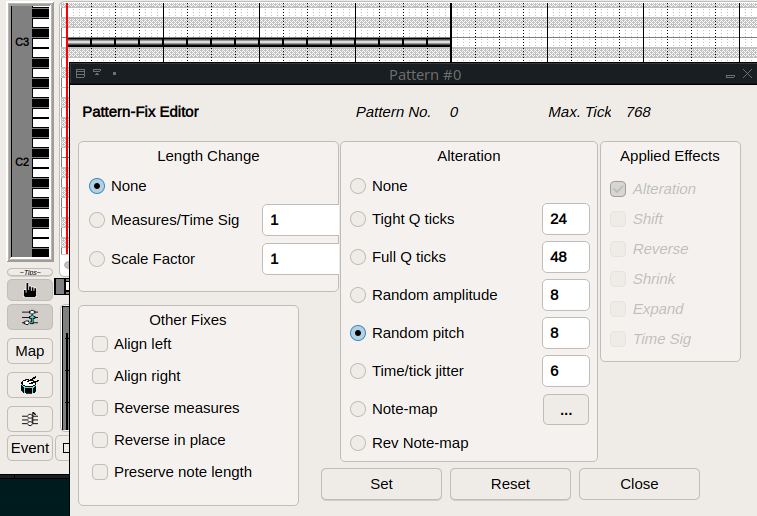
\includegraphics[scale=0.75]{pattern-editor/patternfix-randomize-pitch-setup.png}
   \caption{Pattern Fix Dialog}
   \label{fig:pattern_editor_pattern_fix}
\end{figure}

   \index{pattern-editor!fix}
   When this dialog is used, the time-stamp of \textsl{every event} in the
   pattern can be changed.
   Many other changes can be made as well.
   Once selected, the pattern number is shown in the title-bar and in a
   read-only text field.

   The following sections describe the dialog.
   For more details, go to the source-code bundle, enter the
   \texttt{contrib/notes/} directory, and
   examine the \texttt{pattern-fix-test.text} file.

\subsubsection{Pattern Editor / Pattern Fix / Length Change}
\label{subsubsection:patterns_fix_length_change}

   The \textbf{Length Change} selector allows for the following actions:

   \begin{itemize}
      \item \textbf{None}.
         No length change will occur.
         Alignment, reversing, and quantization can still be done.
      \item \textbf{Measures/Time Sig}.
         Allows the measures (length) of the pattern to be changed in three
         ways, depending on how the number is entered: as an integer or
         floating-point number (e.g. 1, 1.0, 1.75),
         or as a simple time-signature fraction (e.g. "3/4"; the "/" is a
         key indicator of this kind of change).
         In some ways it is similar to \textbf{Scale Factor}, described
         below.
         \begin{itemize}
            \item \textbf{Measures}.
               Entering an integer or a floating-point scale factor will scale
               the pattern events up or down,
               and change the number of measures.
               The final number of measures is always an integer.
               If the measure value is less than \texttt{1.0},
               the pattern will only be compressed.
               If less than 1 measure in length, the result will be
               1 measure; \textsl{Seq66} cannot allow less than 1 measure.
               \textsl{Note that, unlike setting the measures in the pattern
               editor itself, this measures change will \textbf{not}
               truncate notes.}
               If the number of measures is greater, then the notes will
               be expanded.
            \item \textbf{Time Signature}.
               Entering a fraction such as \textbf{3/4} or
               \textbf{12/8} will change the time signature of the pattern
               and scale the pattern down or up appropriately.
               This action can also change the length of the pattern.
         \end{itemize}
      \item \textbf{Scale Factor}.
         Scales the pattern.  For example, 2.0 doubles the length, and 0.5
         halves the length.
         In some ways it is similar to \textbf{Measures}, described
         above.
         The \textbf{Measures} is changed to be enough to contain the new length,
         but only if the scale is greater than 1.0.
         One thing to be aware of is that, if the pattern is expanded, the
         new measure count depends on the location of the last event in the
         expanded pattern.
   \end{itemize}

\subsubsection{Pattern Editor / Pattern Fix / Other Fixes}
\label{subsubsection:patterns_fix_other_fixes}

   \textbf{Other Fixes} provides some minor items, as follows.

   \begin{itemize}
      \item \textbf{Align left}.
         Aligns the pattern to the left (i.e. the beginning)
         of the sequence, removing any delays.
         Useful when recording a pattern live and not quite
         hitting the first beat in time.
      \item \textbf{Align right}.
         Align the pattern to the right of the sequence;
         the last note ends at the end of the sequence.
      \item \textbf{Reverse measures}.
         Reverses all of the events in the whole pattern, flipping the measures
         completely.  For example, if all the events occur near the end of the
         pattern, after reversal they will all appear near the beginning of the
         pattern.
      \item \textbf{Reverse in place}.
         This is probably a more natural reversal method.
         The relative location of a cluster of notes doesn't change, but the
         notes are simply reversed in place.
      \item \textbf{Preserve note length}.
         Prevents Note Offs from being scaled, which shortens or lengthens the
         notes, and in some case might cause notes to bleed past a measure.
         When scaling down, it is usually better to leave this option off.
   \end{itemize}

\subsubsection{Pattern Editor / Pattern Fix / Alteration}
\label{subsubsection:patterns_fix_alteration}

   The \textbf{Alteration} selector allows for various types of
   quantization, randomization, and note-mapping.

   It works similarly to the \textbf{Tool} entries of the
   same name (see \sectionref{subsec:pattern_editor_second_row}),
   but works on \textsl{all events}, not just selected events.
   Also included is a \textbf{Jitter} option, with a range for the jitter.
   This option slightly randomizes the time-stamps of note events.

   \begin{itemize}
      \item \textbf{None}.
      No "alteration" process is done.
      \item \textbf{Tight Q ticks}.
         Quantizes the note times by the amount shown (MIDI ticks)
         in the text-field next to it. Normally, one wants this to be
         half of the next value described.
      \item \textbf{Full Q ticks}.
         Quantizes the note times by the amount shown (MIDI ticks)
         in the text-field next to it. Normally, one wants this to be
         the size of a note, for example, a 16th note, which is 48
         ticks by default.
      \item \textbf{Random amplitude}.
         Randomizes the velocity of notes by plus-or-minus the number of units
         specified in the text-field.
      \item \textbf{Random pitch}.
         Randomizes the pitch of notes by plus-or-minus the number of units
         specified in the text-field.
         The notes adhere to the musical scale set in the pattern
         editor, including the chromatic scale, which includes all twelve
         notes in an octave.
         See \figureref{fig:pattern_editor_pattern_fix}, which shows
         the setup for randomizing the pitches, plus the pattern to be
         randomize.
      \item \textbf{Time/tick jitter}.
         Randomizes the timing of each note by plus-or-minus the number of
         MIDI ticks shown in the text-field.
         Most useful to humanize a too-rigid rhythm.
      \item \textbf{Note-map}.
         Remaps the notes according to a 
         \texttt{.drums} or \texttt{.notemap} file (both are
         identical in concept and layout).
         Unlike the one-the-fly note-mapping capability (where the
         note-map is created at the startup of the application),
         this is a temporary note map.
         The note-map file is read, all notes are re-mapped, and the
         note-map goes away.
         By default the note-map file is the one specified in the 'rc' file,
         though it need not be active for this operation.
         Clicking on the \texttt{...} allows one to select another file to
         use (but only for a pattern-fix).
         The note-map can be used to remap drum notes, or to produce
         special note-remappings, such as inversion.
      \item \textbf{Rev Note-map}.
         This is the same as note-mapping, but maps in the opposite direction.
   \end{itemize}

%  Question:  would a vertical "pattern flip" (of the note values themselves)
%  be useful?

   This figure shows the result of randomizing notes to adhere to a
   Phrygian scale based on C.

\begin{figure}[H]
   \centering 
   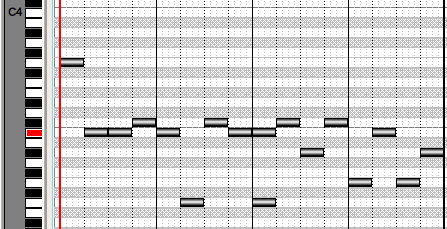
\includegraphics[scale=0.75]{pattern-editor/patternfix-randomize-pitch-result.png}
   \caption{Result of Pattern Fix Note Pitch Randomization}
   \label{fig:pattern_editor_pattern_fix_pitch_randomization}
\end{figure}

\subsubsection{Pattern Editor / Pattern Fix / Applied Effects}
\label{subsubsection:patterns_fix_applied_effects}

   \textbf{Applied Effects} does not do anything except show the effect of the
   changes. The fix process followed is:

   \begin{enumerate}
      \item Apply the left/right-alignment (if selected).
      \item Modify the number of measures (if selected).
      \item Do the scaling (if selected).
      \item Perform the quantization/tightening (if selected).
   \end{enumerate}

   The presumed effect of the change is shown, if applicable.
   Note that changing the measure in this dialog is different from
   changing the measures in the "length" dropdown, which only changes the
   measures.
   Changing the measures to a large number on a pattern of 1 measure will
   greatly expand the notes!

   Any accidental changes can be \textbf{Reset}
   in this dialog.
   Undo in the pattern-editor itself with \texttt{Ctrl-Z} affects
   only MIDI events, not things like the time-signature from the
   drop-downs.

\subsection{Pattern Editor / LFO Dialog}
\label{subsec:pattern_editor_lfo_panel}

   The LFO dialog allows for modulating note velocities and the control values
   of the event type in shown in the data pane.
   It can even modulated tempo events.

   By clicking on the \textbf{LFO} button or using the \texttt{Ctrl-L} key,
   the following window appears, with a set of 4 vertical sliders:

\begin{figure}[H]
   \centering 
  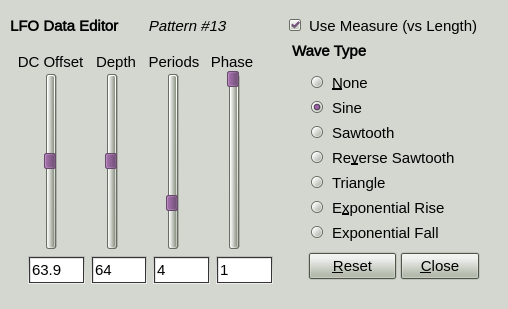
\includegraphics[scale=0.65]{pattern-editor/lfo.png}
   \caption{Pattern Editor LFO}
   \label{fig:pattern_editor_bottom_lfo}
\end{figure}
   
   The user-interface items function as follows.

   \begin{enumber}
      \item \textbf{Use Measures (vs Length)}.
         The length of a waveform period can be determined by the length of the
         pattern (2 measures as shown next to the label "LFO Data Editor") or
         by the length of a measure. This check-box determines that.
         In the diagram, it is checked, so the 2 measures covers four periods
         of the sine wave.
         Especially useful in modifying long patterns.
      \item \textbf{DC Offset} (\textbf{D}).
         Provides a kind of DC offset for the data value. Starts at 64, and
         ranges from 0 to 127.
         In the diagram above, one can see that the "0-value" line for the sine
         wave is at 64.
      \item \textbf{Depth} (\textbf{R}).
         Controls the depth of modulation; i.e. the modulation range.
         Starts at 64, and ranges from 1 to 127.
         The data values range from \( y = DC - R \) to \( y = DC + R\).
%        For the sine-wave shown above, the range is 0 to 128 (actually 127).
      \item \textbf{Periods}.
         Indicates the number of periods per pattern length.
         For long patterns, this parameter should be set high,
         to even show an effect.  It is also subject to an 'anti-aliasing'
         effect, especially for short patterns.
         Try it!
      \item \textbf{Phase Shift} (\textbf{P}).
         Provides the phase shift within a period of the LFO wave.
         A value of 1 is a phase shift of 360 degrees (one whole period).
         Thus, the data at \( P = 0 \) would look exactly the same at phase
         \( P = 1\).
      \item \textbf{Wave Type}.
         Selects the kind of wave to use for the LFO:
         \begin{enumber}
            \item \textbf{None}.
               This setting is useful if one wants to change only the DC
               offset.
            \item \textbf{Sine}.
               Modulates via a sine wave.
               Change the \textbf{Phase Shift} to get a cosine function.
               If the \textbf{DC Offset} is below 64, then negative values are
               converted to positive. As an example, setting the DC offset to 0
               will produce the absolute value of the \texttt{sin()} function.
            \item \textbf{Sawtooth}.
               Provides a ramp modulation.
            \item \textbf{Reverse Sawtooth}.
               Provides a ramp modulation in the opposite direction.
            \item \textbf{Triangle}.
               Modulates via a triangle wave; somewhat similar to a sine wave.
            \item \textbf{Exponential Rise}.
               Provides an exponential ramp modulation.
               This ramping is easiest to see if the DC offset is 0,
               and the Mod range is 127.
               Varying the \textbf{Phase Shift} with the slider
               will move the peak of the curve left to right.
            \item \textbf{Exponential Fall}. Provides a ramp modulation in the
               opposite direction.
         \end{enumber}
         Note that one might have to change one or more parameters
         slightly to see the effect of the new waveform.
      \item \textbf{Reset Data}.
         This button restores the initial pattern event data.  Useful when one
         applies modulation that one ultimately does not like.
      \item \textbf{Close}.  Closes the LFO panel.
   \end{enumber}

   In addition to the \textbf{Reset Data} button, Ctrl-Z can be applied
   multiple times to undo changes one at a time.  Every motion of a control
   causes a complete change.

\subsection{Pattern Editor / Common Actions}
\label{subsec:pattern_editor_common}

   This section is a catch-all for actions not described above.

\subsubsection{Pattern Editor / Common Actions / Scrolling}
\label{subsec:pattern_editor_scrolling}

   \textsl{We still need to work out whether or not to use the scroll wheel.
   in Seq66, as we need to keep multiple event panes in sync while scrolling.}
   Let us describe the actions that can be performed with a
   scroll wheel, or with the scrolling features of multi-touch touchpads.
   There are three major scrolling actions available when using mouse
   scrolling, with the mouse hovering in the piano-roll area:

   \begin{itemize}
      \item \textbf{Vertical Panning (Notes Panning)}
         \index{scroll!normal scroll}
         \index{scroll!vertical pan}
         \index{scroll!notes pan}
         \index{pan!seqroll notes}
         Using the vertical scroll action of a mouse or touchpad moves the
         view of the sequence/pattern notes up and down.
         One can also click in the piano roll, and then use the
         \texttt{Page-Up} \index{keys!page-up}
         and \texttt{Page-Down} \index{keys!page-down}
         keys to move the view up and down in pitch.
      \item \textbf{Horizontal Panning (Timeline Panning)}
         \index{scroll!shift scroll}
         \index{scroll!horizontal pan}
         \index{scroll!timeline pan}
         \index{pan!seqroll time}
         Holding the Shift key, and then using the vertical scroll action of a
         mouse or touchpad moves the view of the sequence/pattern time forward
         and backward.
         One can also click in the piano roll, and then use the
         \texttt{Shift Page-Up} \index{keys!shift page-up}
         and \texttt{Shift Page-Down} \index{keys!shift page-down}
         keys to move the view left and right in time.
      \item \textbf{Horizontal Zoom (Timeline Zoom)}
         \index{scroll!ctrl scroll}
         \index{scroll!horizontal zoom}
         \index{scroll!timeline zoom}
         \index{zoom!seqroll time}
         Holding the Ctrl key, and then using the vertical scroll action of a
         mouse or touchpad zooms the view of the sequence/pattern time to
         compress it or expand it.
         One can also click in the piano roll, and then use the
         \texttt{z} \index{keys!z},
         \texttt{Z} \index{keys!Z}, and
         \texttt{0} \index{keys!0} keys to change the timeline zoom.
      \item \textbf{Vertical Zoom (Notes Zoom)}
         \index{scroll!vertical zoom}
         \index{scroll!notes zoom}
         \index{zoom!seqroll notes}
         Additional buttons for vertical zoom have been added:
         \textbf{-},
         \textbf{0}, and
         \textbf{+}.
         One can also click in the piano roll, and then use the
         \texttt{v} \index{keys!v},
         \texttt{V} \index{keys!V}, and
         \texttt{0} \index{keys!0} keys to change the notes zoom.
         The zoom can make the note-rows large enough to use on a touch screen.
   \end{itemize}

   The actions of this scrolling are smooth and fast.
   If an event is selected in the piano-roll area or the (thin) event area,
   then the scrolling increases or decreases the value of the event.
   In the case of a note, this increases or decreases the velocity of the note.
   For all events, this increases or decreases the length of the vertical line
   that represents the value of the event.

\subsubsection{Pattern Editor / Common Actions / Close}
\label{subsec:pattern_editor_close}

   \index{window!close}
   There is no \textbf{Close} button in the pattern editor.  One can use
   window-manager actions, such as clicking on the \textbf{X}
   button of the window
   frame, or pressing the exit key defined in the window manager.

%-------------------------------------------------------------------------------
% vim: ts=3 sw=3 et ft=tex
%-------------------------------------------------------------------------------


% Song Editor

%-------------------------------------------------------------------------------
% song_editor
%-------------------------------------------------------------------------------
%
% \file        song_editor.tex
% \library     Documents
% \author      Chris Ahlstrom
% \date        2015-08-31
% \update      2025-06-06
% \version     $Revision$
% \license     $XPC_GPL_LICENSE$
%
%     Provides the concepts.
%
%-------------------------------------------------------------------------------

\section{Song Editor}
\label{sec:song_editor}

   The \textbf{Song Editor}
   is also known as the "arrangement panel" or "performance editor".
   The \textbf{Song Editor} combines all patterns
   into a complete tune with controlled repetitions of each pattern.
   It shows one row per pattern/loop/sequence,
   with the placement of each pattern at various and possibly
   multiple time locations in the song.
   \index{performance}
   In \textsl{Seq24} parlance, the song editor creates a
   \textsl{performance}, and the performance is implemented by a set of
   triggers.
   Triggers are internal timing items stored with each pattern when a
   \textsl{Seq66} MIDI tune is saved.
   \index{song mode}
   In \textbf{Song} mode, these triggers, not the user, control
   playback.

   \begin{quotation}
      \textbf{Tip}
      In the installed \texttt{data/midi} directory, there are sample files for
      the tunes "Europe Endless" and "Peter Gunn" that illustrate what can be
      done with the song editor.  They are accompanied by descriptive text
      files.  Be sure to check them out.
   \end{quotation}

   \index{song editor!dual}
   Two song editor windows can be
   brought onscreen, one in the \textbf{Song} tab, and
   one in an external window.
   The \textbf{Song} tab and a \textbf{Song} window can be shown at the
   same time.

%  The \textbf{Song} editor activates
%  the \textbf{Song} mode of \textsl{Seq66}.
%  When the song editor has the focus of the application, it
%  takes over control from the patterns panel, and controls playback.

   Once playback is started in the song editor (using the \texttt{Space} or
   \texttt{.} keys), live mode is disabled.
   The song editor takes over the arming/unarming (unmuting/muting)
   shown in the patterns panel.  The highlighting of armed/unarmed patterns
   changes according to whether the pattern is triggered in the song editor.
   If one tries to change the muting in
   the patterns panel, the song editor immediately returns the pattern to the
   state it has in the song editor.  The only way to manually change the muting
   then is to click the pattern's label in the song editor.
   Both the song editor and the patterns panel both reflect the change in
   muting in the user-interface.

\begin{figure}[H]
   \centering 
   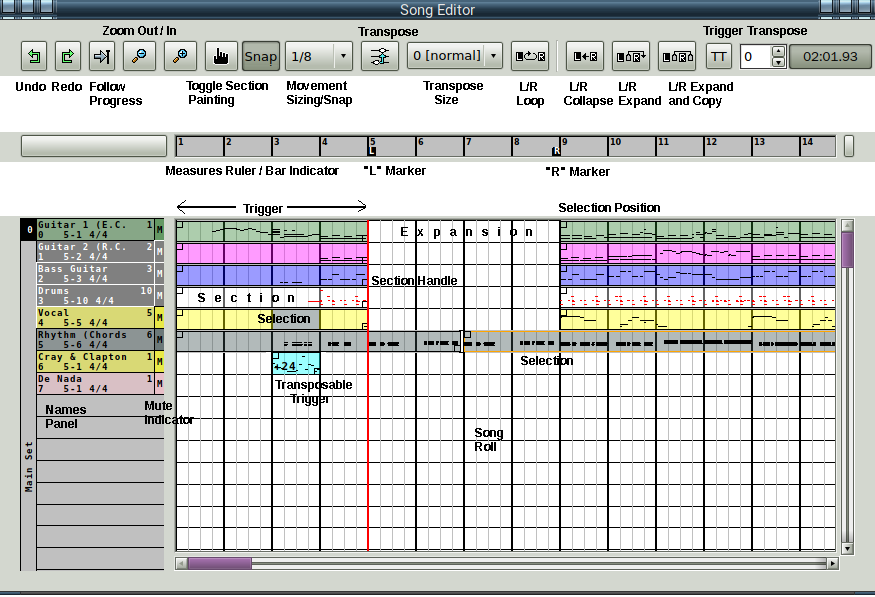
\includegraphics[scale=1.0]{song-editor/song-editor-annotated.png}
   \caption{Song Editor Window, Annotated}
   \label{fig:song_editor_window_annotated}
\end{figure}

   This is another diagram one might want to print out for reference.
   Note the major items shown:

   \begin{enumber}
      \item \textbf{Top Panel} (recent updates not yet shown)
      \item \textbf{Measures Ruler}
      \item \textbf{Patterns (Names) Panel}
      \item \textbf{Song Roll}
      \item \textbf{Bottom Panel}
   \end{enumber}

   The estimated duration of the tune appears at the right of the top panel.
   It is calculated from the length of patterns
   and the song triggers that may be present.
   Here are some of the features for the song editor:

   \begin{itemize}
      \item Toggling of the mute state of multiple patterns
         via the name fields of the patterns.
      \item Optional pattern coloring (selected in the Patterns panel)
      \item A configurable progress bar.
      \item \textbf{Undo} and \textbf{Redo} buttons.
      \item A \textbf{Transpose} button and transposition drop-down selector.
      \item Red coloring of events for patterns that are not transposable,
         such as drum tracks.
      \item Horizontal zoom (and a simple vertical zoom)
      via buttons and keystrokes.
      \item Opening a pattern editor via a double-click on any occupied
         track.
      \item Creating a pattern via a double-click on any unoccupied track.
   \end{itemize}

   The song editor is a bit complex; for exposition, we break it into
   sections, starting with playback keystrokes.

\subsection{Song Editor / Playback Keystrokes}
\label{subsec:song_editor_playback_keystrokes}

   The song roll (center panel)
   of the song editor provides keystrokes for starting,
   stopping, and pausing playback.
   Other keystrokes are described in
   \sectionref{subsubsec:song_editor_song_roll_keystrokes}.

%  \itempar{Stop}{song editor!stop}
%  Stops the playback of the song.
%  \index{keys!esc (stop)}
%  The keystroke for stopping playback is the \texttt{Esc} character.
%  It can be configured to be another character (such as \texttt{Space}, which
%  would make the space-bar toggle the playback status).

%  \itempar{Stop/Pause/Play}{song editor!play}
   \index{keys!space (toggle play)}
   The keystroke for starting playback is the \texttt{Space} character.
   \index{L marker}
   It starts the playback of the song at the \textbf{L marker}.
   The \textbf{L marker} serves as the start position for playback
   in the song editor.  One can change the start position only when the
   performance is not playing.
   The \texttt{Space} character also toggles playback.
   This character also rewinds the song to the beginning when stopping.

   Another keystroke for stopping playback is the \texttt{Esc} character.
   This character also rewinds the song to the beginning when stopping.
   (It also can exit paint mode, and,
   \textsl{if} the 'usr' \texttt{[pattern-editor] escape-pattern}
   option is set, will close an external song-editor window.

   \index{keys!period (pause)}
   The keystroke for pausing playback is the \texttt{Period} character.
   When used, it keeps the progress at the same spot as before.

   Note that there are no stop, pause, and play buttons in the
   song editor.
   They are provided by the main window.
   The \textbf{Song} tab can be activated in the main window to
   keep the playback buttons nearby.

\subsection{Song Editor / Top Panel}
\label{subsec:song_editor_top}

   The top panel shown earlier provides quick access to actions
   and configuration.

   \begin{enumber}
      \item \textbf{Undo}
      \item \textbf{Redo}
      \item \textbf{Follow Progress}
      \item \textbf{Zoom Out and Zoom In}
      \item \textbf{Toggle Selection/Trigger Painting}
      \item \textbf{Record Snap}
      \item \textbf{Grid Snap}
      \item \textbf{Transpose}
      \item \textbf{L/R Loop}
      \item \textbf{L/R Collapse}
      \item \textbf{L/R Expand}
      \item \textbf{L/R Expand and Copy}
      \item \textbf{Expand Song Roll} (not shown in figure)
      \item \textbf{Trigger Transpose}
      \item \textbf{Song Duration}
   \end{enumber}

   \setcounter{ItemCounter}{0}      % Reset the ItemCounter for this list.

   \itempar{Undo}{song editor!undo}
   The \textbf{Undo} button rolls back the last change in the layout of a
   pattern.  Each time it is clicked, the most recent change is undone.
   Also implemented via \texttt{Ctrl-Z}.

   \itempar{Redo}{song editor!redo}
   The \textbf{Redo} button reapplies the last change undone by
   the \textbf{Undo} button.
   Also implemented via \texttt{Shift-Ctrl-Z}.

   \itempar{Follow Progress}{song editor!follow}
   Toggles the mode of following progress
   for longer songs.  WHen active, the song roll pages right to keep up with
   the progress bar.

   \itempar{Zoom Out/Zoom In}{song editor!zoom}
   These buttons change the horizontal zoom.
   Zoom can also be changed via the keystrokes \texttt{z}, \texttt{0},
   and \texttt{Z}.
   Vertical zoom is also supported, by buttons to the left of the time-line and
   by keystrokes, as discussed below.

   \itempar{Toggle Selection/Trigger Painting}{song editor!paint}
   Toggles the ability
   to drag the mouse along the pattern's timeline to create triggers
   to indicate when the pattern will play.
   Short patterns will be duplicated one or more times as
   the mouse is dragged.
   This mode can alsp be changed via the keystrokes \texttt{p} ("paint"),
   \texttt{i} ("insert"), \texttt{x} ("excape").and \texttt{Esc}.

   \itempar{Grid/Record Snap}{song editor!grid/record snap}
   The \textbf{Movement Sizing/Snap} setting,
   if enabled, allows not only full clips of a pattern to be added,
   but smaller intervals listed below.
   It turns on record-snap for recording live performance triggers.
   It also enables the grid snap functionality,
   which ndicates the horizontal grid snap for movement actions and trigger
   drawing.
   If disabled, it allows the trigger to be placed and to be smoothly extended
   in either direction, without snapping, when the mouse is moved left or
   right. It allows exact recording of the musician's arming/muting of
   patterns.
   Unlike the \textbf{Grid Snap} of the pattern editor, the units
   of the song editor snap value are in fractions of a measure length.
   The following values are supported:

   \textsl{1/1, 1/2, 1/4, 1/8, 1/16, and 1/32}

   Note that arming/muting can be done in the "names" panel using a
   \textsl{right-click} on the pattern name.
   Also note that changes that occur within the snap value will 
   cause odd recording, so be sure to set the snap value low enough.

   When creating triggers for patterns longer than a measure,
   the pattern may wrap, so that beginning notes appear at the end of the
   trigger, and notes can wrap around.
   To avoid this, a trick is needed:

   \begin{enumerate}
      \item Undo that trigger insertion.
      \item Select the \texttt{Length} Snap value.
      \item Insert the trigger.
      \item Click another snap value.
      \item Drag the trigger, usually to the left, until it reaches the
         desired snap location.
      \item Verify that the whole pattern is in place with the notes exactly
         placed as in the pattern.
   \end{enumerate}

   This trick is annoying, and we're not sure if note wrap-around
   is a feature or a bug.

   \itempar{Transpose}{song editor!transpose}
   \index{global transpose}
   \textbf{Transpose} consists of two controls:
   a combo-box to select the transpose direction and amount,
   and a \textbf{TT} button to reset the transposition value to 0.
   Global (song) ransposition ranges from -12 to +12.
   It can be locked in using the
   \textbf{Edit / Apply Song Transpose} menu entry.

   \itempar{L/R Loop}{song editor!play loop}
   This button is also present in the main window.
   It sets up playback to move only between the "L" and "R" markers.
   For a description of this button, see
   \sectionref{subsubsec:introduction_loop_button}.

   \itempar{L/R Collapse}{song editor!collapse}
   This button collapses the song between the \textbf{L marker} and the
   \textbf{R marker}.
   What this means is that, if there is song material (patterns) before the
   \textbf{L marker} and after the \textbf{R marker},
   and the \textbf{Collapse} button is
   pressed, any song material between the L and R markers is erased, and
   the song material after the \textbf{R marker} is moved leftward to
   the \textbf{L marker}.
   Collapsing occurs in all tracks present in the song editor.

   \itempar{L/R Expand}{song editor!expand}
   This button expands the song between the
   \textbf{L marker} and the \textbf{R marker}.
   It inserts blank space between these markers, moving the song material
   that is after the \textbf{R marker}
   to the right by the duration of the blank space.
   Expansion occurs in all tracks present in the song editor.

   \itempar{L/R Expand and Copy}{song editor!expand and copy}
   This button expands the song between the \textbf{L marker} and the
   \textbf{R marker} much like the \textbf{Expand} button.
   However, it also copies the original data that is present after the
   \textbf{R marker}, and pastes it into the newly-available space between
   the L and R markers.

   \itempar{Expand Song Roll}{song editor!expand song roll}
   Sometimes one might come to the end of the song and still want to
   add more triggers.
   Clicking this button expands the song roll to the right, adding
   more room for triggers.

   \itempar{Trigger Transpose}{song editor!trigger transpose}
   Not to be confused with song transpose,
   this button and spin-box make trigger selections or segments
   transposable during play-back.  This feature is very useful
   for patterns that repeat many times, but are shifted in pitch at various
   points.
   The transposition value ranges from -60 to 0 to +60, in units of semitones.
   The button resets the value to 0.
   To apply a transposition value, first set it in the spin-box.
   Then carefully \textsl{shift-left-click}
   on the desired segment(s) to transpose.
   A number with a plus-or-minus will appear at the left of the segment to
   indicate a non-zero transposition.
   The transposition value will be saved with the trigger when the song is
   saved.

   For a good example, see the \textsl{Kraftwerk "Europe Endless"}
   demonstration MIDI file in the \texttt{data/midi} directory.

   \itempar{Song Duration}{song editor!duration}
   Shows the full duration of the song based on the longest pattern or
   the trigger layout.
   Toggle between H:M:S and B:B:T notation by clicking on it.

\subsection{Song Editor / Measures Ruler}
\label{subsec:song_editor_measures_ruler}

   \index{measures ruler}
   The measures ruler ("bar indicator", or "Time")
   consists of a \textsl{timeline} at the top and the 
   \textbf{L marker} and \textbf{R marker} mentioned above.
   It also includes an \textbf{END} marker to indicate the
   end of the song.
   The \textsl{measures ruler} is the ruled and numbered section at the top
   of the arrangement panel.  It provides a place to put the left and right
   markers.  In the \textsl{Seq24} documentation, it is called the "bar
   indicator".
   There are some hidden details (tricks) in the measures panel used to
   set the markers and the current play-head position.

   \begin{itemize}
      \item \textbf{In the upper half} of the time-line,
         the mouse pointer changes to a vertical pointer.
         Clicking there then shows a red dot; these mark
         the starting position of playback.
         This is useful for review.
      \item \textbf{In the lower half} of the time-line,
         the mouse pointer changes to a "finger" icon.
         \textsl{Left-clicking} there then moves the \textbf{L}
         marker to that point.
         \textsl{Right-clicking} there moves the \textbf{R} marker to that point.
         (\textbf{R} will never precede \textbf{L}, though).
         If the \textbf{Loop} button in the main window is active, then
         playback will loop between the \textbf{L} and \textbf{R} buttons.
         This looping now works with both Live and Song modes.
   \end{itemize}

   \index{measures ruler!left-click}
   \textsl{Left-click} in the bottom-half of the
   measures ruler to move and drop an
   \index{L anchor}
   \index{L marker}
   \textbf{L marker} (\textbf{L anchor}) on the measures ruler.
   \index{measures ruler!right-click}
   \textsl{Right-click} in the bottom-half of the measures ruler to drop an
   \index{R anchor}
   \index{R marker}
   \textbf{L marker} (\textbf{R anchor}) on the measures ruler.
   
   These markers denote the time interval from the left of the 
   \textbf{L} marker to the right of the \textbf{R} marker.
   Once these markers are in place, one can then use
   the \textsl{Collapse} and \textsl{Expand} buttons to modify the
   placement of the pattern events.
   Note that the \textbf{L marker} serves as the start position for playback
   in the song editor even when not looping.
   One can change the start position only when the
   performance is not playing.

   \index{marker!mode}
   \index{marker!movement}
   Another way to move the \textbf{L} and \textbf{R} markers has been added.
   To select which marker will move, click the upper half of the time
   strip (otherwise, the \textbf{L} will move,
   prematurely) to give it keyboard focus.
   Then press the lower-case
   \index{keys!l}
   \texttt{l} key or the lower-case
   \index{keys!r}
   \texttt{r} key.
   \textsl{There is no visual feedback that one is in the movement mode.}
   Then press the \texttt{Left-Arrow} or \texttt{Right-Arrow}
   key to move the selected marker.
   Also included at the same level as the measures ruler are the buttons
   \textbf{-}, \textbf{0}, and \textbf{+},
   which are used for vertical zoom, as described below.

\subsection{Song Editor / Pattern Names Panel}
\label{subsec:song_editor_patterns_panel}

   The patterns panel is at the left of the song roll.
   Here are the items to note in the pattern-names panel:

   \begin{enumber}
      \item \textbf{Number}.
         The number of the screen-set.
      \item \textbf{Title}.
         \index{pattern!title}
         \index{pattern!name}
         The title is the name of the pattern, for easy reference.
      \item \textbf{Color}.
         If a color is provided for the pattern, then that color is shown.
         Also, as an editing aid, the pattern over which the mouse is hovering
         is shown in a brighter version of the color.
      \item \textbf{Measures}.
         \index{pattern!channel}
         The number of measures in the pattern appears
         at the right of the title.
      \item \textbf{Pattern Number}.
         The pattern number is on the left of the second line of text.
      \item \textbf{Buss-Channel}.
         \index{pattern!buss-channel}
         This pair of numbers shows the MIDI buss number used in the pattern
         and the channel used for the pattern.
      \item \textbf{Beat/Measure}.
         \index{pattern!beat}
         This pair of numbers is the standard time-signature of the pattern.
      \item \textbf{Trigger Count}.
         \index{pattern!trigger count}
         This number shows the number of triggers present in the pattern.
      \item \textbf{Mute Indicator}.
         \index{song editor!mute indicator}
         The letter \textbf{M} is in a grey box if the track/pattern
         is muted via song playback,
         and a white (or colored) box if it is unmuted in song playback.
         \textsl{Left-clicking} on the \textbf{M} (or the name of the pattern)
         mutes/unmutes the pattern.
         \index{left click}
         Song muting is effected via a \textsl{left-click} on the pattern name.
         This is also useful in song-recording (where the triggers are recorded).
         \index{shift left click}
         If the Shift key is held while \textsl{left-clicking}
         on the M or the pattern name, then
         the mute/unmute state of every other active pattern is toggled.
         This feature is useful for isolating a single track or pattern.
         \index{right click}
         Normally, one records song triggers using the grid buttons or MIDI
         control to turn patterns on and off.
         One can also \textsl{right-click} on the pattern
         name during song-record and
         thereby see the trigger(s) being created.
      \item \textbf{Empty Track}.
         Completely empty tracks (no track events or meta events)
         are indicated by a dark-gray filling in the pattern column.
         Tracks that have only meta information, but no playable event, are
         indicated by a yellow filling in the pattern column.
   \end{enumber}

   The patterns column shows a list of all of the patterns that have been
   created in the current song.  Each pattern in this list has a track of
   pattern layouts associated with it in the piano roll section.

   \index{patterns column!left-click}
   \index{patterns column!ctrl-left-click}
   \index{song editor!muting}
   \textsl{Left-clicking} on the pattern name or the \textbf{M} toggles the muting
   (arming) status of the track.
   It does the same thing if the \texttt{Ctrl} key is held at the same time.

   \index{pattern!shift-left-click}
   \index{song editor!inverse muting}
   \index{song editor!solo}
   \index{shift-left-click solo}
   \textsl{Shift-left-clicking} on the pattern name
   or the \textbf{M} button toggles the muting
   (arming) status of \textsl{all other tracks} except the track that was
   selected.  This action is useful for quickly listening to a single sequence
   in isoloation.

   \index{patterns column!double-click}
   \textsl{Double-clicking} on the pattern name
   will either create a new pattern or open up the corresponding pattern
   window.
   This feature saves having to move to the live grid.

% Think about implementing this feature for real. At least partially.
%
%  \index{patterns column!right-click}
%  \textsl{Right-clicking} on the pattern name or
%  the \textbf{M} button brings up the same
%  pattern editing menu as discussed in
%  \sectionref{subsubsec:patterns_pattern_filled}.
%  Recall that this context menu has the following entries:
%  \textbf{Edit...}, \textbf{Event Edit...}, \textbf{Cut}, \textbf{Copy},
%  \textbf{Song}, \textbf{Disable Transpose}, and \textbf{MIDI Bus}.

\subsection{Song Editor / Song Roll}
\label{subsec:song_editor_song_roll}

   The "Song Roll" section of the arrangement panel is where patterns or
   subsections are inserted, deleted, shrunk, lengthened, or moved.
   Actions can be done via the mouse or keyboard.

   \textbf{Warning}.
   There is a horizontal and a vertical scrollbar for the song roll.
   However, some patterns may hide the scrollbars or obscure them.
   For example, the Qt "kvantum" themes replace the scrollbar
   with just its "thumb", and show it in the roll, but only when the
   mouse is near the bottom or right borders.
   Weird!

\subsubsection{Song Editor / Song Roll / Layout}
\label{subsubsec:song_editor_song_roll_layout}

   The song/piano roll provides one line (track) per pattern.
   It provides another way (besides the live grid) to control
   and lay out patterns.
   Patterns can be set up with multiple triggers and can be
   brought up for editing.
   Here are features to note in the annotated piano roll area:

   \begin{enumber}
      \item \textbf{Note Events}.
         \index{song editor!note events}
         Note in the pattern are shown as thin horizontal lines.
         They can be edited in the pattern editor's piano roll,
         and in the event editor.
      \item \textbf{Tempo Events}.
         \index{song editor!tempo events}
         Tempo events in the pattern are shown as very small squares.
         They can be edited in the pattern editor's data panel,
         and in the event editor.
      \item \textbf{Pattern Access}.
         Double-click-edit (if enabled in the 'rc' file) on a track
         representing an existing pattern will bring up an external
         pattern editor windows.
         Double-clicking on an empty track will create a new pattern
         and bring up its pattern editor.
         This new functionality is merely for convenience.
      \item \textbf{Trigger Creation}.
         By click-dragging the mouse on a track, in paint mode,
         a series of triggers can be
         created; they indicate where the track will be unmuted and playing.
         See below for more information about triggers.
      \item \textbf{Selection}.
         Clicking inside a trigger selects it.
         Selection is denoted by
         an orange color in the trigger.
         A pattern subsection selection can be moved clicking and holding
         the mouse near the middle of the selection first.
         A pattern subsection selection can be deleted by keystrokes.
         At present, selection of more than one trigger at a time (via
         drawing a rectangle on them) is \textsl{not supported}.
      \item \textbf{De-selection}.
         \index{song editor!section deselection}
         \textsl{Left-clicking} or \textsl{right-clicking} in
         an empty area of the song roll
         will deselect the selection.
      \item \textbf{Selection Movement}.
         \index{song editor!selection movement}
         If one grabs (\textsl{left-click}) inside
         the pattern or pattern subsection, that item can be moved
         horizontally via the left and right arrow keys,
         as long as there is room.
      \item \textbf{Section Length ("handle")}.
         \index{song editor!handle}
         \index{song editor!section length}
         The small squares in two corners of the patterns are the section
         "handles".
         By grabbing a handle with a \textsl{left-click},
         the handle can be moved
         horizontally to either lengthen or shorten the pattern to the nearest
         snap position, if there is room to move in the desired direction.
      \item \textbf{Pattern Subsectioning}.
         \index{song editor!split pattern}
         \index{song editor!middle click}
         \index{pattern subsection}
         A \textsl{middle-click} (or \textsl{ctrl-left-click})
         inside a pattern inserts a selection position
         marker in it, breaking the pattern into two equal pieces.
         This division can be done over and over.
         There are also options for splitting at the nearest snap point.
         See below.
      \item \textbf{Expansion}.
         \index{song editor!section expansion}
         Originally, all the long patterns of this sample song were continuous.
         But, by setting the L and R markers, and using the \textbf{Expand}
         button, we opened up some silent space in the song, just to be able
         to show it off.
   \end{enumber}

   The \textsl{Seq24} help files refer to work in the song editor as the
   "Performance Editor" or "Performance Mode".  Adding a pattern in this
   window is a bit like adding a note in the pattern editor.
   One clicks, holds, and drags the mouse to insert a copy or copies of the
   pattern associated with the row in which one is dragging.
   The longer one drags, the more copies of the pattern that are inserted.

   \index{song editor!right-click-hold}
   \index{song editor!draw}
   \index{paint mode}
   \textsl{Right-click} on the arrangement panel (roll) to enter
   paint mode, and hold the button.
   Paint mode does not work while the sequence is playing.
   Another way to turn on painting is to
   make sure that the performance editor piano roll has the
   keyboard focus by \textsl{left-clicking} in it, then press the
   \texttt{p} or \texttt{i} key to enter the paint/insert mode, and
   \texttt{x} (or \texttt{Esc} if not playing) to escape it.
   See \sectionref{subsubsec:song_editor_song_roll_keystrokes}.

   \index{zoom}
   \index{song editor!horizontal zoom}
   The song editor supports horizontal zoom in the piano roll.
   This feature is accessible via the "magnifying glass" buttons, and also
   accessible via the keystrokes \textbf{z}, \textbf{0}, and \textbf{Z}.
   The zoom feature also modifies the time-line.

   \index{zoom}
   \index{song editor!vertical zoom}
   The song editor supports limited vertical zoom in the piano roll.
   This feature is accessible via the \textbf{-}, \textbf{0}, and
   \textbf{+} buttons, and also
   accessible via the keystrokes \textbf{v}, \textbf{0}, and \textbf{V}.

   \index{song editor!left-click-right-hold}
   \index{song editor!insert}
   A \textsl{left-click} with a simultaneous
   \textsl{right-click-hold} inserts one copy of the
   pattern.  The inserted pattern shows up as a box with a tiny
   representation of the notes visible inside.  Some patterns can
   be less than a measure in length, resulting in a tiny box.
   \index{song editor!right-left-hold-drag}
   \index{song editor!multiple insert}
   To keep adding more copies of the pattern, continue to hold both buttons
   and drag the mouse rightward.

   \index{song editor!middle-click}
   \textsl{Middle-click} (or \textsl{ctrl-left-click})
   on a trigger in a pattern row
   to splits the trigger into two triggers.
   \index{pattern!split}
   \index{song editor!pattern subsection}
   This splits the pattern into two equal \textsl{pattern subsections}.
   Each \textsl{middle-click} on the pattern adds a new selection position,
   halving the size of the subsections as more pattern subsections are
   added.  The \texttt{allow\_snap\_split} option in the 'rc' file
   allows the split to be made at the nearest snap point instead of in the
   middle.

   \index{song editor!left-click}
   \index{song editor!selection}
   When a pattern or a pattern subsection is
   \textsl{left-clicked} in the piano
   roll, it is marked with an orange background.
   It can then be moved horizontally if there is room, or be deleted or copied
   for later pasting.

   \index{song editor!right left click}
   \index{song editor!deletion}
   When a 
   \textsl{right-left-click} action is done in this gray area, the result
   is to \textsl{delete} that pattern section or subsection.
   \index{keys!delete}
   One can also hit the \texttt{Delete} key.

   \index{song editor!double-click}
   \textsl{Double-click} on one of the trigger bars
   will either create a new pattern or open up the corresponding pattern
   window.
   This feature saves having to move to the live grid.

\subsubsection{Song Editor / Song Roll / Keystrokes}
\label{subsubsec:song_editor_song_roll_keystrokes}

   There are a number of useful keystrokes in the song roll that can be used
   once is has focus, by clicking in it.

   \begin{itemize}
      \item Enter "paint" mode.
         The \texttt{p} or \texttt{i} keys enter paint mode,
         where additional triggers
         can be added by click-dragging on a pattern row.
         The \texttt{x} or \texttt{Esc} keys leave this mode.
         The "finger" button and the mouse cursor both indicate the status.
      \item Start/Pause button functionality.
         When the song roll has keyboard focus,
         the \texttt{Space} key starts and stops playback, rewinding to the
         beginning when stopped.
         The \texttt{.} (period) key starts and pauses playback, without
         rewinding.
         This functionality is similar to that of the main window, but
         these keys are not reconfigurable in the song roll.
      \item Undo / Redo / Cut / Copy / Paste of a selected section.
         Provided by buttons and by these keystrokes:
         \begin{itemize}
            \item \texttt{Ctrl-Z}. Undo.
            \item \texttt{Shift-Ctrl-Z}. Redo.
            \item \texttt{Ctrl-X}. Cut.  Removes the selection.
            \index{keys!backspace}
            \index{keys!delete}
            \index{keys!ctrl-x}
            Can also be done with the \texttt{Delete} and
            \texttt{Backspace} keys.
            The deletion can be undone.
            \item \texttt{Ctrl-C}. Copy.
         \index{keys!ctrl-c}
         \index{keys!copy}
            Copies the trigger for later usage.
            \item \texttt{Ctrl-V}. Paste.
            \index{keys!ctrl-v}
            \index{keys!paste}
            Puts the roll into paste mode.
            When inserted, each insert goes immediately
            after the current item or the previous insertion.  The same can be
            done for whole patterns.
         \end{itemize}
      \item Horizontal (Time) Zoom.  These keystrokes work similarly to the
      pattern editor's piano roll.
         Provided by buttons and by these keystrokes:
         \index{keys!shift-z}
         \texttt{Z}. Zoom in horizontally (i.e. in time).
         \index{keys!z}
         \texttt{z}. Zoom out horizontally.
         \index{keys!0}
         \texttt{0}. Reset zoom both horizontally and vertically.
      \item Vertical (Time) Zoom.  These keystrokes work similarly to the
         pattern editor's piano roll.
         However, there are only three levels of
         vertical zoom:  half-size, normal, and double-size.
         \index{keys!shift-V}
         \texttt{V}. Zoom in vertically to get a better view of the patterns
            and a large grab handle.
         \index{keys!v}
         \texttt{v}. Zoom out vertically to see more tracks.
         \texttt{0}. Reset zoom both horizontally and vertically.
      \item Scrolling Horizontally/Vertically.
         \index{keys!arrows}
         The arrow keys will move the piano row up, down, left, and right.
         \index{keys!hjkl}
         In addition, the "vi" keys \texttt{h}, \texttt{j}, \texttt{k}, and
         \texttt{l} will act like the arrow keys.
         The mouse scroll wheel can also be used to move the panes around.
         For implementation reasons, the scroll wheel is active
         \textsl{only} in the piano roll.
      \item Jumping to the Beginning/End.
         \index{keys!Home}
         \index{keys!End}
         The \texttt{Home} and \texttt{End} keys act as normal, jumping to the
         beginning or end of the song roll
         The \texttt{Ctrl-Home} key acts just like \texttt{Home}.
         The \texttt{Ctrl-End} key is like \texttt{End}, but it leaves the
         end of the song in view in the middle of the song roll.
      \item Paging.
         One can page up and down vertically in the arrangement
         panel using the
         \index{keys!page-up}
         \texttt{Page Up} and 
         \index{keys!page-down}
         \texttt{Page Down} keys.
         One can page left and right horizontally in the arrangement
         panel using the
         \index{keys!up-arrow} \texttt{Up-Arrow} and 
         \index{keys!down-arrow} \texttt{Down-Arrow} keys.
   \end{itemize}

\subsection{Song Editor / Bottom Panel}
\label{subsec:song_editor_bottom}

   The bottom panel is simple, consisting of a stock horizontal scroll bar.

\begin{comment}

   ...and a small button, called the \textbf{Grow} button, labelled with a
   "\textbf{$>$}".
   \index{grow button}
   \index{song editor!grow}
   The \textbf{Grow} button adds to the number of measures that exist
   in the song editor. The visual effect is very subtle, resulting only
   in a small change in the thumb of the horizontal scroll-bar, unless one
   is at the right end of the piano roll.  Then, one can see the added
   measures.  Usually about 128 at a time are added, but this depends on the
   value of PPQN in force.

\end{comment}

%-------------------------------------------------------------------------------
% vim: ts=3 sw=3 et ft=tex
%-------------------------------------------------------------------------------


% Event Editor

%-------------------------------------------------------------------------------
% event_editor
%-------------------------------------------------------------------------------
%
% \file        event_editor.tex
% \library     Documents
% \author      Chris Ahlstrom
% \date        2016-01-02
% \update      2025-06-07
% \version     $Revision$
% \license     $XPC_GPL_LICENSE$
%
%-------------------------------------------------------------------------------

\section{Event Editor}
\label{sec:event_editor}

   The \textsl{Seq66} \textbf{Event Editor} tab is used to view and edit,
   in detail, the events present in a loop / sequence / pattern / track.
   It is accessed by right-clicking on a pattern in the \textbf{Live} frame,
   then selecting the \textbf{Edit pattern in tab} menu entry.
   The default keystroke combination for this action is to use the
   \textsl{minus} key followed by the desired pattern's hot-key.

   The event editor is not very sophisticated.
   It is a basic editor for simple edits, viewing, and trouble-shooting.
   It is disabled if recording a pattern, to avoid refresh issues while
   recording.

   Viewing and scrolling work;
   editing, deleting, and inserting events work.
   But there are many possible interactions between event links
   (Note Off events linked to Note On events, for example),
   performance triggers, and the pattern,
   performance, and event editor dialogs.
   Surely some bugs still lurk.
   If anything bad happens, do \textsl{not} press the
   \textbf{Save to Sequence} button!
   If the application aborts, let us know!
   Here are the major "issues":

   \begin{enumerate}
      \item It requires the user to know the details
         about MIDI events and data values.
      \item For safety, it does not detect any changes made to the sequence in
         the pattern editor; we might add a refresh button.
      \item It does not have an undo function. Just don't save!
      \item It cannot mark more than one event for deletion or modification.
         However, if one note event is deleted, the corrsponding linked note
         event is also deleted.
      \item There is no support for dragging and dropping of events.
   \end{enumerate}

   The event editor is a good way to see the events in a sequence,
   and to delete or modify problematic events.
   Additionally, it can be used to add \textbf{Set Tempo} and other
   meta events.
   \index{sequence extension}
   \index{pattern extension}
   If an event is added that has a time-stamp beyond the current
   length of the sequence, then the length of the sequence is extended.
   Unlike the event pane in the pattern editor, the event-editor
   dialog shows all types of events at once.

\begin{figure}[H]
   \centering
   \includegraphics[scale=0.65]{event-editor/event-editor-tab.png}
   \caption{Event Editor Window}
   \label{fig:event_editor_window}
\end{figure}

   The event-editor dialog is fairly complex.
   For exposition, we break it down into a few sections:

   \begin{enumber}
      \item \textbf{Event Frame}
      \item \textbf{Info Panel}
      \item \textbf{Edit Fields}
      \item \textbf{Bottom Buttons}
   \end{enumber}

   The event frame is a list of events, which can be traversed, and edited.
   The fields in the right panel show the name of
   the pattern containing the events and other information about the
   pattern.  The edit fields provide text fields for viewing and entering
   information about the current event, and buttons to delete, insert, and
   modify events.  The bottom buttons allow changes to be saved and the editor
   to be closed.  
   The following sections described these items in detail.

\subsection{Event Editor / Event Frame}
\label{subsec:event_editor_frame}

   The event frame is the event-list shown on the left side of the
   event editor.  It is accompanied by a vertical scroll-bar, for moving one
   line or one page at a time.
   Mouse or touchpad scrolling can be used to move up and down
   in the event list.
   Depending on the window manager theme, the currently-selected event
   is highlighted.
   (We have been trying to get this table to auto-stretch vertically when the
   main window is vertically maximized, but have not succeeded so far. Qt!)

\subsubsection{Event Frame / Data Items}
\label{subsec:event_frame_data}

   The event frame shows a list of numbered events, one per line.
   The currently-selected event is shown in the edit fields.
   Here is an example of the data line for a MIDI event:

   \begin{verbatim}
      17   003:3:128 Note On -- 3  69 107 003:4:96
   \end{verbatim}

   This line consists of the following parts:

   \begin{enumber}
      \item \textbf{Index Number}
      \item \textbf{Time Stamp}
      \item \textbf{Event Name}
      \item \textbf{Bus Number} (new)
      \item \textbf{Channel Number}
      \item \textbf{Data Bytes D0 and D1}
      \item \textbf{Link}
   \end{enumber}

   \setcounter{ItemCounter}{0}      % Reset the ItemCounter for this list.

   \itempar{Index Number}{event editor!index number}
   Displays the index number of the event.
   This number is purely for reference, and is not part
   of the event.  Events in the pattern are numbered from 1 to the number of
   events in the pattern.

   \itempar{Time Stamp}{event editor!time stamp}
   Displays the time stamp of the event,
   which indicates the cumulative time of the event in the pattern.
   It is displayed in the format of "measure:beat:divisions" (e.g. B:B:T).
   The measure values start from 1, and range up to the number of measures in
   the pattern.
   The beat values start from 1, and range up to the number of beats in the
   measure.
   The division values range from 0 up to one less than the
   \index{ppqn}
   PPQN (pulses per quarter note) value for the whole song.
   \index{ppqn!\$ shortcut}
   As a shortcut, one can use the dollar sign ("\$") to represent
   PPQN-1.
   If the \textbf{Tick Time} box is checked, then the timestamps are
   shown in units of "ticks" (MIDI pulses, also called "divisions").

   \itempar{Event Name}{event editor!event name}
   Displays the name of the event.
   The event name indicates what kind of MIDI event it is. 
   See \sectionref{subsec:event_editor_fields}.

   \itempar{Bus Number}{event editor!bus number}
   Shows the bus that the event came in on, or a hyphen if not applicable.
   This value is currently not saved with the event,
   so is of limited utility.

   \itempar{Channel Number}{event editor!channel number}
   Shows the channel number (for channel-events only) re 1, not 0.
   (For the user, MIDI channels always range from
   1 to 16.  Internally, they range from 0 to 15.)

   \itempar{Data Bytes D0 and D1}{event editor!data bytes}
   Shows the one or two data bytes for the event.
   The byte is shown in one two formats, hexadecimal and decimal, depending
   on the setting of the \textbf{Hex} check-box.
   For text events, a small portion of the text is shown.
   The full text is shown in the text field below the D0 and D1 values.

   Note Off, Note On, and Aftertouch events requires a byte for the key (0 to
   127) and a byte for the velocity (also 0 to 127).
   Control Change events require a control code and a value for that control
   code.  Pitch wheel events require two bytes to encode the full range of
   pitch changes.
   Program change events require only a byte value to pick the patch or program
   (instrument) to be used for the sequence.  The Channel Pressure event
   requires only a one-byte value.
   Tempo requires a number (e.g. "120.3") to be typed in.

   \itempar{Links}{event editor!links}
   Note events are linked together; each Note On is linked to the corresponding
   Note Off, and vice versa.

\subsubsection{Event Frame / Navigation}
\label{subsec:event_frame_navigation}

   Moving about in the event frame is straightforward, but has some
   wrinkles to note.
   Navigation with the mouse is done by moving to the desired event and
   clicking on it.  The event becomes highlighted, and its data items are shown
   in the "info panel".
   There is no support for dragging and dropping events in the event frame.
   There is no support for selecting multiple events.

   The scrollbar can be used to move within the frame, either by one line at a
   time, or by a page at a time.  A page is defined as one frame's worth of
   lines, minus 5 lines, for some overlap in paging.

   Navigation with keystrokes is also supported, for the Up and Down arrows and
   the Page-Up and Page-Down keys.  Note that using the Up and Down arrows by
   holding them down for awhile causes autorepeat to kick in.
   Use the scrollbar or page keys to
   move through multiple pages.  Home and End also work.

\subsection{Event Editor / Info Panel}
\label{subsec:event_editor_info}

   The "info panel" is a read-only list of properties on the top right
   of the event editor.  It serves to remind the used of the pattern being
   edited and some characteristics of the pattern and the whole song.
   It also includes one button.
   Five items are shown:

   \begin{enumber}
      \item \textbf{Sequence Number and Name}.
         A bit redundant, as the window caption or the pattern
         also shows the pattern name.
         It can be set here or in the pattern editor.
      \item \textbf{Sel Linked}. (Not shown in picture.)
         If this button is checked, then selecting a Note On or Off event
         also selects the opposite, linked note.
         This allows for easy deletion of a complete Note pair.
      \item \textbf{Channel Number}.
         Shows the output channel number.
      \item \textbf{Time Signature}.
         A pattern property, shown only as a reminder.
         It can be set in the pattern editor.
      \item \textbf{PPQN}.
         Shows the "parts per quarter note", or resolution of the
         whole song.  The default PPQN of \textsl{Seq66} is 192.
      \item \textbf{Sequence Channel}.
         In \textsl{Seq66}, the channel number is a property of the
         pattern.  All channel events in the pattern get routed to the same
         channel, even if somehow the event itself specifies a different
         channel.
      \item \textbf{Sequence Count}.
         Displays the current number of events in the pattern.
         This number changes as events are inserted or deleted.
   \end{enumber}

\subsection{Event Editor / Edit Fields}
\label{subsec:event_editor_fields}

   The edit fields show the values of the currently-selected event.  They allow
   changing an event, adding a new event, or deleting the currently-selected
   event. These have been greatly updated for user convenience in the last
   few releases of \textsl{Seq66}.

   \begin{enumber}
      \item \textbf{Category}.
         This dropdown shows what kind of event is selected, and can
         also be used to insert specific events. The event categories are:
         \begin{itemize}
            \item \textbf{Channel Message}.
            \item \textbf{System Message}.
            \item \textbf{Meta Event}.
            \item \textbf{SecSpec Event}.
         \end{itemize}
         See below for more information about supported events.
      \item \textbf{Time}.
         Shows the event timestamp in B:B:T notation.
         It can be edited to move an event in time.
      \item \textbf{Event}.
         This dropdown shows the event name.
         It can also be used to select an event that is appropriate for
         the selected event category.
      \item \textbf{D0}.
         Shows data byte 1, e.g. the note number for a note event.
         It can also be edited.
      \item \textbf{D1}.
         Shows data byte 2, e.g. the velocity for a note event.
         It can also be edited.
      \item \textbf{Tick Time}.
         If check-marked, the \textbf{Time} column in the event list
         is shown as ticks (pulses, divisions) instead of B:B:T.
      \item \textbf{Hex}.
         If check-marked, the \textbf{D0} and \textbf{D1} columns
         in the event list, as well as the editable
         \textbf{D0} and \textbf{D1} fields, as shown in hexadecimal notation.
         For example, D0 = 67 is shown as "0x43".
      \item \textbf{Text}.
         This field is for the display of certain events, such as
         pitch data. It is also used for entering text data for various
         text events.
   \end{enumber}

   \textbf{Important}: changes made in the event editor
   are \textsl{not written} to the sequence until the \textbf{Save}
   button is clicked.  If one messes up an edit field, just click on the event
   again; all the fields will be filled in again.
   That's as much "undo" as the event-editor offers at this time, other than
   closing without saving.

   \setcounter{ItemCounter}{0}      % Reset the ItemCounter for this list.

   \itempar{Category}{event editor!event category}
   Displays the event category of the event.
   All channel events, most system messages
   and many meta events can be handled,
   even system-exclusive events.

\begin{figure}[H]
   \centering
   \includegraphics[scale=0.65]{event-editor/message-category-dropdown.png}
   \caption{Event Category List}
   \label{fig:event_editor_category_dropdown}
\end{figure}

   There are four types of messages handled by \textsl{Seq66}:
   Channel, System, Meta, and SeqSpec. 
   Seqspec messages are stored when a pattern is saved, but they are
   not part of the pattern's event list.
   Hence this item is grayed out; these message values are shown in various
   parts of the user interface.
   See the table in \sectionref{subsec:midi_format_meta_format}.

   \itempar{Time}{event editor!event timestamp}
   Displays the timestamp of the selected event in B:B:T format.
   "measure:beat:division" format is fully supported.
   We allow editing (but not display) of the timestamp in
   pulse (divisions) format and "hour:minute:second.fraction" format, but
   there may be bugs to work out.

   If one wants to delete or modify an event, this field does not need to be
   modified. If this field is modified, and the \textbf{Modify}
   button is pressed, then the event will be moved  This field can locate
   a new event at a specific time.  If the time is not in the current frame,
   the frame will move to the location of the new event and make it the current
   event.

   \itempar{Time}{event editor!event time}
   Shows the time of the event in the format of "measure:beat:divisions" (only).
   This field can be edited to change the time of the event.

   \itempar{Event}{event editor!event name}
   Displays the name of the event, and allows entry of an event name.
   The event name indicates what kind of MIDI event it is. 
   The following event names are supported for Channel events:

   \begin{enumber}
      \item \textbf{Note Off}
      \item \textbf{Note On}
      \item \textbf{Aftertouch}
      \item \textbf{Control}
      \item \textbf{Program}
      \item \textbf{Channel Pressure}
      \item \textbf{Pitch Wheel}
   \end{enumber}

   Selecting one of these names from the dropdown changes the kind of event if
   the event is modified.
%  Abbreviations and case-insensitivity can be used to
%  reduce the effort of typing.
%  Also, if \textbf{Control} or
%  \textbf{Program} are selected, then a data drop-down box is available
%  to select either the controller or
%  the instrument patch (program), and it can fill in the data values.
   If \textbf{Control} or \textbf{Program} are selected,
   then the name of item-number entered into \textbf{D0} is
   shown in the text area.

   In the future, we may make these configurable and add selection
   drop-downs, with the control-change
   following the settings in the 'usr' file, and the program-change being made
   from a (new) 'patches' file.
   Currently the programs are General MIDI.

   If the \textbf{Meta Event} category is selected, the following events are
   shown:

\begin{figure}[H]
   \centering
   \includegraphics[scale=0.75]{event-editor/meta-event-dropdown.png}
   \caption{Meta Event List}
   \label{fig:event_editor_meta_dropdown}
\end{figure}

   If the \textbf{System Message} category is selected, the following events are
   shown:

\begin{figure}[H]
   \centering
   \includegraphics[scale=0.85]{event-editor/system-event-dropdown.png}
   \caption{System Message List}
   \label{fig:event_editor_system_dropdown}
\end{figure}

   At present, many of these messages, especially the textual messages,
   should be editable.
   Report any issues.

   \itempar{Channel}{event editor!channel}
   This dropdown shows the channel of the current event, ranging from 1 to 16.
   If the event is not a channel message, then \textbf{None} is shown.

   \itempar{D0}{event editor!data byte 1}
   Allows modification of the first data byte of the event.
   One must know what one is doing.
   The scanning of the digits is very simple:  start with the first digit, and
   convert until a non-digit is encountered.  The data-byte value can be
   entered in decimal notation, or, if prepended with "0x", in hexadecimal
   notation.
   For \textbf{Control} or \textbf{Program},
   the name of item-number in \textbf{D0} is
   shown in the text area.

   For a Tempo setting only this field is used; Data Byte 2 is ignored.
   Enter a Tempo value, such as "120", and then click \textbf{Insert}. The
   value is converted to the 3 bytes of a tempo event, and then
   added at the given timestamp.  (Screen refresh is not perfect yet, but
   reloading the pattern shows the correct tempo.)

   \itempar{D1}{event editor!data byte 2}
   Allows modification of the second data byte of the event (if applicable
   to the event).
   One must know what one is doing.
   The scanning of the digits is as noted above.

   \itempar{Tick time}{event editor!tick time}
   Selecting this check-box
   shows the time-stamps in the frame in tick (pulses) format.

   \itempar{Hex}{event editor!hex data}
   Selecting this check-box
   shows all number items in hex format.

   \itempar{Text data}{event editor!text data}
   This unlabelled pane shows the text of a meta text event.
   This field can be edited to add or change a meta text event.
   The events supported are:
   \textsl{Text Event},
   \textsl{Copyright},
   \textsl{Instrument Name},
   \textsl{Lyric},
   \textsl{Program Name}, and
   \textsl{Device Name}.
   It also shows translated versions of the control or program numbers in
   \textbf{D0}.

%  \itempar{Delete}{event editor!delete event}
%  Causes the selected event to be deleted.
%  The frame display is updated to move following events upward.

\subsection{Event Editor / Bottom Buttons}
\label{subsec:event_editor_buttons}

   These are the buttons that act on the edit fields or current event
   selection:

   \begin{enumber}
      \item \textbf{Delete}.
         Delete the selected event.
      \item \textbf{Insert}.
         Create a new event based on the data in the fields.
      \item \textbf{Modify}.
         Officially modify the selected event.
      \item \textbf{Clear}.
         Clear all events.
      \item \textbf{Save}.
         Save all the changes back to the pattern.
      \item \textbf{Dump}.
         Dump the events to a file.
   \end{enumber}

   Note that
   \index{bugs!event delete key}
   \index{bugs!event insert key}
   \textsl{Seq66} does not support using the
   \texttt{Delete} and \texttt{Insert} keys to
   supplement the buttons; the \texttt{Delete}
   key is needed for editing the event data fields.

   \setcounter{ItemCounter}{0}      % Reset the ItemCounter for this list.

   \itempar{Insert}{event editor!insert event}
   Inserts a new event, described by the 
   \textbf{Event Timestamp},
   \textbf{Event Name},
   \textbf{Data Byte 1}, and
   \textbf{Data Byte 2} fields.
   The new event is placed in the appropriate location for the given timestamp.
   If the timestamp is at a time that is not visible in the frame, the frame
   moves to show the new event, so be careful.

   \itempar{Modify}{event editor!modify event}
   Deletes the current event, and inserts the modified event,
   which is placed in the appropriate location for the given
   timestamp.  (This feature does not work with linked Note Ons and Note Offs).

   \itempar{Clear}{event editor!clear events}
   Deletes all of the events in the event table.
   As with all edits, does not become official until the \textbf{Save} button
   is clicked.

   \itempar{Save}{event editor!save events}
   Saves all of the events in the event table into the original sequence.
   There is no way to undo this action.
   This button does not close the dialog; further
   editing can be performed.  The Save button is enabled only if
   some unsaved changes to the events exist.
   Any sequence/pattern editor that is open should be reflected
   in the pattern editor once this button is pressed.

   \itempar{Dump}{event editor!dump events}
   Write the events to a text file in the same directory as the MIDI file, very
   useful for troubleshooting.  The name of the file is of the form:

   \begin{verbatim}
      midi_file_name-pattern-#.text
   \end{verbatim}

   where '\#' is the pattern number.  For example, if the loaded file is

   \texttt{/home/user/miditunes/The\_Wild\_Bull.midi}

   and the pattern is 9, then the resulting dump-file is

   \texttt{/home/user/miditunes/The\_Wild\_Bull-pattern-9.text}.

%-------------------------------------------------------------------------------
% vim: ts=3 sw=3 et ft=tex
%-------------------------------------------------------------------------------


% Session Management

%-------------------------------------------------------------------------------
% seq66 sessions
%-------------------------------------------------------------------------------
%
% \file        sessions.tex
% \library     Documents
% \author      Chris Ahlstrom
% \date        2020-10-03
% \update      2025-06-07
% \version     $Revision$
% \license     $XPC_GPL_LICENSE$
%
%  Provides a discussion of how Seq66 supports session management, specifically
%  the Non Session Manager.
%
%-------------------------------------------------------------------------------

\section{Session Management}
\label{sec:sessions}

   A session is a group of applications and their configuration and
   connections.
   Session management recreates complex setups and provides some uniformity
   of application control in a session.
   The first thing to do for session management is to make sure that the
   application is capable of various levels of session management, from
   \textsl{UNIX} signals to
   a complete session manager like the \textsl{Non/New Session Manager}.
   Basic session management consist of being able to properly start the
   application and let it run properly during its life-cyle, whether it is a
   command-line application or a graphical application.
   \textsl{Seq66} supports session management in three ways:

   \begin{enumber}
      \item \textbf{Signals}.
         During a normal run, \textsl{Seq66} will respond
         to signals to save and to quit.
         The normal configuration files and command-line options will be
         used, and can be marked to be saved at exit.
         This mode is useful with \textsl{nsm-proxy}, a way to script
         applications that don't have \textsl{NSM} support.
      \item \textbf{JACK Session}
         Deprecated, but implemented nonetheless.
         Many still use it.
         This session manager allows the configuration files to be stored in
         a separate directory, for \textsl{Seq66} to be started, and files to
         be saved.  No restrictions on where the MIDI files can be stored.
      \item \textbf{Non Session Manager}
         Known as \textsl{NSM}, and in the form of a fork of that project,
         \textsl{New Session Manager},
         it provides a replacement for \textsl{JACK Session}.
         It requires all files to be
         stored in a session directory, and provides commands for saving,
         quitting, hiding/showing the user-interface, and more.
         Like \textsl{JACK Session}, it allows control over the startup of
         multiple applications, the process of saving a session, and provides a
         way to save their patching (connections) in \textsl{JACK}.
         However, it supports more functionality and has
         strict requirements the application must follow.
         Development of NSM has, for various reasons, been suspended, but
         offshoots such as \textsl{Agordejo} (\cite{agordejo})
         and \textsl{RaySession} (\cite{raysession}), which are front ends for
         the \textsl{New/Non Session Manager} (\cite{nsm}),
         continue to advance.
   \end{enumber}

   For session management, \textsl{NSM} is the way to go.
   \textsl{JACK} session management is provided for those who still use it.
   There are other session solutions, such as \textsl{aj-snapshot},
   \textsl{Claudia}, and \textsl{Chino}.
   For now, we do not discuss them.

   The desired session can be set in the \textbf{Edit / Preferences /
   Session} tab.  But note that, if started by \textsl{NSM}, \textsl{Seq66}
   will detect it and nonetheless set up for NSM usage.
   The \textsl{NSM} setting is
   useful for attaching to a pre-existing known session.
   \textsl{JACK} session management events are processed
   only if \textsl{JACK} is selected.
   \textsl{JACK} session management will still start \textsl{Seq66} in
   an existing session, if \textsl{JACK} is
   not selected.

   Also note that sometimes one will want the session manager to make the JACK
   connections.  In this case, go to
   \textbf{Edit / Preferences / JACK / Jack Auto-Connect}, uncheck that option,
   and restart \textsl{Seq66}.
   This option, \texttt{jack-auto-connect}
   can also be changed in the 'rc' file.
   The \textsl{NSM} tool called \textsl{jackpatch} can also be used to manage
   connections.

\subsection{Session Management / Signals}
\label{subsec:sessions_signals}

   \index{sessions!signals}
   By default, the basic form of session management in
   \textsl{Seq66} occurs by signals.  A
   session manager can start \textsl{Seq66}, and it can tell \textsl{Seq66} to
   save or stop.  Starting is done by a system call to spawn the application.
   The save and stop actions are supported by sending the following signals to
   the application:

   \begin{itemize}
      \item \texttt{SIGINT}.
         This signal stops \textsl{Seq66}. It corresponds
         to using \texttt{Ctrl-C} from the command-line to stop \textsl{Seq66}.
         This signal should work for both the graphical and command-line
         application.  As \textsl{Seq66} shuts down, it does its normal saving
         of the current state of the configuration.
      \item \texttt{SIGTERM}.
         This signal also stops \textsl{Seq66}.  It can
         be sent by an application to exit \textsl{Seq66}.
      \item \texttt{SIGUSR1}.
         This signal tells \textsl{Seq66} to save.  This
         action will save the current MIDI file.
   \end{itemize}

   One application that can control \textsl{Seq66} via these signals, when not
   in session mode, is \textsl{nsm-proxy}:

      \url{https://non.tuxfamily.org/wiki/nsm-proxy}

   \textsl{NSM-Proxy} is a simple \textsl{NSM} client for wrapping non-NSM
   capable programs. It enables the use of programs supporting LADISH Level 0
   and 1, and programs which accept their configuration via command-line
   arguments.  There is a command-line version and a graphical version.
%  More to come on how to use \texttt{nsm-proxy}.

\subsection{Session Management / JACK Session}
\label{subsec:sessions_jack}

   Although deprecated by the \textsl{JACK} authors in favor of \textsl{NSM},
   we are implementing \textsl{JACK} session (JS) management for the benefit of
   people who either do not know of \textsl{NSM} or do not want to implement or
   use it.

   \textsl{Seq66}, as a JS-aware applications, is set up to

   \begin{enumerate}
      \item Register with a JS manager.
      \item Respond to messages from the JS manager.
      \item Be startable with session information.
   \end{enumerate}

   A response to a JS message will do one of the following:

   \begin{itemize}
      \item Save the application's state into a file, where the directory is
         supplied by the session manager.
      \item Reply to the session manager with a command-line that starts the
         application, with information to restore its state, such as
         the name of the file holding its state information.
   \end{itemize}

	JS-aware clients identify themselves to the session manager by a UUID
	(unique universal identifier). The session manager provides it to
	the client application as an integer represented as a string.
   This can be passed to the session manager when registering, but
   \textsl{Seq66} just uses the value given to it (for now).

%  but should also be passed back to the client when it is restarted
%by the session manager. This is done by a command line argument to the
%application, and the format of the command line is also up to the client.

   For this discussion, we will use the \textsl{JACK} session implementation in
   the \textsl{QjackCtl} application.
   Also, read the script stored in
   \texttt{seq66/data/linux/jack/startqjack} to set up
   \textsl{QjackCtl} to run \textsl{JACK} and kick off
   \textsl{a2jmidid}; it should be added to the \textsl{QjackCtl}
   configuration.
   A more recent script,
   \texttt{seq66/data/linux/jack/jackctl}, is what we tend to use, but not
   for this demonstration.

   Once that setup is made (installing the script and configuring
   \texttt{qjackctl}, then start \texttt{qjackctl}.
   Verify that there are a number of system audio and MIDI playback and capture
   port, \textsl{PulseAudio JACK} sinks and sources if the system uses
   \textsl{PulseAudio}, and that there are "a2j" MIDI ports for all of your USB
   hardware devices.

   Then start \textsl{Qsynth} so it uses \textsl{jack} for MIDI and
   \textsl{jack} (or \textsl{pulseaudio}) for audio.
   Then run \textsl{Seq66} with \textsl{JACK} for slave transport and for MIDI
   (either command works the same):

   \begin{verbatim}
      $ qseq66 --jack-slave --jack-midi
      $ qseq66 --jack-slave --jack
   \end{verbatim}

   Load a file, make sure its MIDI output goes to "fluidsynth" or "qsynth", and
   plays.
   In your desired location (e.g. \texttt{~/.config/seq66/sessions},
   create a new session directory (e.g. \texttt{qtest}).

   In \textsl{qjackctl}, open the \textbf{Sessions} dialog.
   Click \textbf{Save}, and choose the directory just created.
   In the dialog should appear entries for MIDI capture and playback for
   "fluidsynth" and "seq66", all the "a2j" USB devices,
   plus an entry for \textsl{JACK} client
   \textsl{seq66master} or \textsl{seq66slave} that shows
   something like:

   \begin{verbatim}
qseq66 --jack --jack-master --jack-session-uuid 84670 --home ${SESSION_DIR}
qseq66 --jack --jack-slave --jack-session-uuid 84670 --home ${SESSION_DIR}
   \end{verbatim}

   In the \textbf{Connections} dialog of \textsl{QjackCtl}, all of these ports
   will be shown in the MIDI tab, auto-connected appropriately.
   In the sessions directory that was created, will be seen an
   empty \texttt{seq66master}
   or \texttt{seq66slave} directory, and a
   \texttt{sessions.xml} configuration file containing the information shown in
   the sessions dialog.
   Exit \textsl{Seq66}, \textsl{QSynth} and \textsl{QjackCtl}
   (in that order).

   One issue is that \textsl{QSynth}
   does not support \textsl{JACK Session}.
   Try it with \textsl{Yoshimi}, which does support it.

\subsection{Seq66 Session Management / NSM}
\label{subsec:sessions_nsm}

   \index{sessions!nsm}
   The \textsl{Non Session Manager} is an API implementation for session
   management for Linux audio/MIDI.
   \textsl{NSM} clients use a well-defined
   \index{sessions!OSC}
   \textsl{OSC} protocol (\cite{osc})
   to communicate with the session management daemon.
   Note that \textsl{Non Session Manager} is in a state of suspended
   development, and has been reimplemented as a \textsl{GitHub} project,
   the \textsl{New Session Manager}.

   The applications it manages should be installed normally (that is,
   for system-wide usage, in
   \texttt{/usr/bin/} or \texttt{/usr/local/bin}).
   Other locations, if used, must be added to the \texttt{PATH}
   environment variable.

   The following is the recommended setup for get ready for
   NSM usage:

   \begin{itemize}
      \item Set up all of the \textsl{hardware} MIDI input and output ports,
         including USB MIDI.
      \item Start JACK. Important!
         The \texttt{jackctl} script can be used
         to start (and stop) JACK and to run \textsl{a2jmidid}.
      \item Start the JACK-using software synthesizers.
      \item Run \textsl{Seq66} stand-alone after installation.
      \item Set it to use JACK for MIDI (and also for Transport,
         if desired).
      \item If the NSM program \textsl{jackpatch} is going to be used
         for saving and restoring connections, make sure that
         \textsl{Seq66}'s auto-connect feature is \textsl{disabled}.
         Another option is to use \textsl{virtual ports} (the "manual" option
         where the user makes the connections).
      \item Run one of the following GUI applications to create a
         new NSM session: \textsl{agordejo}; \textsl{raysession}; or
         the legacy NSM application.
      \item Once the session is running, verify the ports and MIDI
         settings that have been copied from
         \textsl{\textasciitilde/.config/seq66} to
         \textsl{\textasciitilde/.local/share/nsm/sessionname}.
   \end{itemize}

\subsubsection{Session Management / NSM / First Run Without NSM}
\label{subsec:sessions_nsm_first_run_without_nsm}

   This section discusses what happens when \textsl{Seq66} is installed, then
   run outside of any session from the console or an application menu.
   For a discussion where \textsl{Seq66} is run for the first time under
   \textsl{NSM},
   see \sectionref{subsec:sessions_nsm_first_run_in_nsm}.

   Generally, after installing \textsl{Seq66}, or when creating a new setup
   (such as a play-list) it is good to run it normally first, to simplify
   trouble-shooting.
   This action creates the configuration files in the default location,
   \texttt{/home/user/.config/seq66}:

\begin{verbatim}
   $ qseq66 
   No 'rc' file, will create: qseq66.rc/ctrl/midi/mutes
   No 'usr' file, will create: /home/user/.config/seq66/qseq66.usr
   File exists: /home/user/.config/seq66/qseq66.rc
   Saving initial config files to session directory!
   Writing 'rc': /home/user/.config/seq66/qseq66.rc
   Writing 'ctrl': /home/user/.config/seq66/qseq66.ctrl
   Writing 'mutes': /home/user/.config/seq66/qseq66.mutes
   Writing 'usr': /home/user/.config/seq66/qseq66.usr
   . . .
\end{verbatim}

   Then exit \textsl{Seq66} to ensure the configuration files are created.
   Optionally, in this initial setup,
   one can also create a 'playlist' file and a 'drums' file, or
   copy them from:

   \begin{verbatim}
      /usr/share/seq66-0.91/data/samples
   \end{verbatim}

   to

   \begin{verbatim}
      /home/user/.config/seq66
   \end{verbatim}

   and modify them appropriately.
   Another first-time modification to consider is setting up \textsl{Seq66} to
   use the \textsl{JACK} audio/MIDI subsystem (on \textsl{Linux}).
   In the 'rc' file, look for the following line:

   \begin{verbatim}
      [jack-transport]
      jack-midi = false
   \end{verbatim}

   And change it to:

   \begin{verbatim}
      [jack-transport]
      jack-midi = true
   \end{verbatim}

   Another first-time modification to consider is using virtual ports (option
   \texttt{-{}-manual-ports}) versus the automatic port connections
   \textsl{Seq66} normally makes.
   This setup allows the user to manually make connections between
   \textsl{Seq66} and other MIDI applications.
   In the 'rc' file, look for the following lines:

\begin{verbatim}
   [manual-ports]
   virtual-ports = false   # 'true' = manual (virtual) ALSA or JACK ports
   output-port-count = 8   # number of manual/virtual output ports
   input-port-count = 4    # number of manual/virtual input ports
\end{verbatim}

   And change the virtual-ports line to:

\begin{verbatim}
   [manual-ports]
   virtual-ports = true    # 'true' = manual (virtual) ALSA or JACK ports
\end{verbatim}

   Most of these settings can be made in \texttt{Edit / Preferences}.

   It is then important to start \texttt{qseq66} in the normal manner again,
   and verify that everything works as expected.

   We have added a command, \textbf{File / Import / Project Configuration}
   command to import the configuration files from one directory into the
   current \textsl{NSM} session configuration directory.
   This import used to be automatic, but is too surprising to an unsuspecting
   user.

\subsubsection{Seq66 Session Management / NSM / Run in NSM}
\label{subsec:sessions_nsm_first_run_in_nsm}

   Note: When \textsl{Seq66} is run in \textsl{NSM} for the first time,
   a stock default configuration is saved when
   \textsl{Seq66} exits.
   This is different from earlier behavior, where the home configuration was
   imported automatically.
   Now, the user must use the
   \textbf{File / Import / Project Configuration...}
   command to import an existing setup..

   For illustration, we run \textsl{NSM} from a terminal window, which can be
   very helpful when problems occur.

\begin{verbatim}
   $ non-session-manager
   [non-session-manager] Starting daemon...
   [nsmd] Session root is: /home/user/NSM Sessions
   NSM_URL=osc.udp://mycomputer.mls:19625/
   [nsmd] Listing sessions
\end{verbatim}

   \index{sessions!non-starter}
   \index{sessions!liblo library}
   If \textsl{NSM} refuses to start, make sure that the \texttt{liblo} library
   from the OSC project is installed.
   \index{sessions!/etc/hosts}
   \index{sessions!loopback interface}
   If it is installed, then check the
   \texttt{/etc/hosts} file to make sure that a loopback interface is
   defined. In some versions of \textsl{Linux}, it isn't defined properly,
   and the \textsl{NSM} daemon (\texttt{nsmd}) will not start.
   Here is an example of the loopback installed in \textsl{Debian Sid};

\begin{verbatim}
   127.0.0.1   localhost
   127.0.1.1   mycomputer.mls mycomputer
\end{verbatim}

   The NSM user-interface (not shown here) that comes up is empty at first.
   So create a session by clicking the \textsl{NSM}
   \textsl{New} button, and entering a session name
   (here, "\textbf{Seq66}") in the
   prompt that comes up.  In the console window, a couple of 
   \texttt{/nsm/server/new} \textsl{OSC} messages
   about the creation of the session appear.

\begin{verbatim}
   [non-session-manager] Sending new for: Seq66
   [nsmd] Creating new session "Seq66"
   [non-session-manager] /nsm/server/new says Created.
   [non-session-manager] /nsm/server/new says Session created
\end{verbatim}

   Next, click the \textsl{Add Client to Session}, and, since
   \texttt{qseq66} has been installed system-wide, it is in the \texttt{PATH}
   and its executable name can be entered simply: "\texttt{qseq66}".
   A number of console messages from
   \textsl{Seq66} appear, plus some messages from \textsl{NSM}.

\begin{verbatim}
   [non-session-manager] Sending add for: qseq66
   [nsmd] Process has pid: 2797436
   [nsmd] Launching qseq66
   [nsmd] Got announce from seq66
   [nsmd] Client was expected.
   [nsmd] Process has pid: 2797436
   [nsmd] The client "seq66" at "osc.udp://127.0.0.1:13318/" informs us it's
    ready to receive commands.
\end{verbatim}

   Important: the \textsl{Seq66} user-interface will not show at first.
   It is hidden so that the screen is not inundated with the windows of all the
   applications that are (eventually) running under the session.
   This is especially annoying with tiled window managers.
   In order to see the \textsl{Seq77} user-interface, click on
   the \textbf{GUI} button in the session line shown in the \textsl{NSM}
   window to make \textsl{Seq66} visible.

   Once \textsl{Seq66} is running under \textsl{NSM},
   then click the \textbf{Save}
   button at the top of the \textsl{NSM} interface in order
   to save the session information.
   This is an \textsl{important} step.
   After \textsl{Seq66} exits,
   one can see what has been created to support the session;
   the directory that \textsl{NSM}
   creates by default is \texttt{/home/user/.local/share/nsm}.
   (It used to be \texttt{/home/user/NSM Sessions}.)
   \index{nsm!old session}

\begin{verbatim}
   $ pwd
   /home/user/.local/share/nsm
   $ lstree Seq66
   Seq66/
     +-- seq66.nGJDW/
     |   +-- config/
     |   |   +-- qseq66.ctrl
     |   |   +-- qseq66.drums
     |   |   +-- qseq66.mutes
     |   |   +-- qseq66.palette
     |   |   +-- qseq66.playlist
     |   |   +-- qseq66.rc
     |   |   +-- qseq66.usr
     |   +-- midi/
     +-- session.nsm
\end{verbatim}

   \textbf{Reminder}: If one is running a recent "New" version of the 
   \textsl{Non Session Manager}, then the session data is not stored
   in \texttt{/home/user/NSM Sessions},
   but in
   in \texttt{/home/user/.local/share/nsm},
   \index{nsm!new session}

   So \textsl{NSM} has created a directory with the session name we gave it:
   \texttt{Seq66}.

   \textsl{Side note: the \texttt{nsmd} daemon creates a file named after its
   process ID in \texttt{\$XDG\_RUNTIME\_DIR/nsm/d}, e.g.
   \texttt{/run/usr/1000/nsm/d/2170}.}

   Under that directory is a file, \texttt{session.nsm}, which
   contains information like the following:

\begin{verbatim}
   seq66:qseq66:nGJDW
\end{verbatim}

   The format of this text is \texttt{appname:exename:nXYZT}, where
   \texttt{XYZT} is a 4-letter randomly-generated token
   generated by \textsl{NSM}.
   Also created is a directory, \texttt{seq66.nXYZT}, which is the root of the
   \texttt{Seq66} session.

   The rest of the directories,
   \texttt{config} and \texttt{midi},
   are generated by \textsl{Seq66}
   The \texttt{config} directory is used instead of
   \texttt{/home/user/.config/seq66}) and the \texttt{midi} directory
   contains new MIDI files, imported MIDI files,
   or MIDI files from a play-list.
   The new \texttt{config} directory
   contains versions of the various configuration files that will always be
   used to start up \textsl{Seq66} during the session.
   One can also add valid play-list, palette, and drums/note-mapping files to
   that directory later.

   If before running \textsl{NSM},
   one had set up a play-list file and provided the proper "MIDI
   base directory" in the 'rc' file, then all the MIDI files are copied to
   the \textsl{NSM} session \texttt{midi} directory,
   preserving all relative directories.
   When the \textsl{Non Session Manager} is started the next time, and the
   "Seq66" session is clicked, this starts \textsl{Seq66}, and the play-list can
   be seen in the \textsl{Playlist} tab.

   Note that the \textbf{Save} button on the session's row in the
   \textsl{NSM} user-interface sends a message to \textsl{Seq66}
   to tell it to save its state.

   One last thing to note is that, when viewing the MIDI ports created by
   \textsl{Seq66}, they will be named "seq66" when not in session management,
   and "seq66.nXYZT" (for example) when under session management.  This makes
   it possible to run multiple instances of \textsl{Seq66}.

\subsubsection{Session Management / NSM / Run with Remote NSM}
\label{subsec:sessions_nsm_before_using_nsm}

   As described in the \textsl{NSM} documentation, the \texttt{nsmd} daemon can
   be run stand-alone, and can also be ran on a remote computer.
   The \texttt{qseq66.usr} file can be edited to allow \textsl{Seq66} to
   use a pre-planned \textsl{NSM} and specify the URL to connect.
   Look for the following lines in the 'usr' file:

   \begin{verbatim}
      [user-session]
      session = none
      url = ""
   \end{verbatim}

   Now assume we've run the daemon as follows:

   \begin{verbatim}
      $ nsmd --osc-port 9999
      [nsmd] Session root is: /home/user/NSM Sessions
      NSM_URL=osc.udp://mycomputer.mls:9999/
   \end{verbatim}

   Change the \texttt{session} lines to allow the usage of
   \textsl{NSM} at that URL:

\begin{verbatim}
   [user-session]
   session = nsm
   url = "osc.udp://mycomputer.mls:9999"
\end{verbatim}

   The \texttt{url} is not used if running \textsl{Seq66} from the \textsl{NSM}
   GUI... the application will get the URL from the \textsl{NSM} environment.
   Note that \texttt{qseq66} can still be run outside of a
   session manager.  It will detect the absense of the session manager and run
   normally.

\subsubsection{Session Management / Sessions Tab}
\label{subsubsec:sessions_tab}

   The \textsl{Session} tab is a mostly \textsl{read-only} tab
   provided to orient the user to the setup supported by the session.
   When not running in a session, the normal configuration directory and files
   are shown.  When running in an \textsl{NSM} section, the configuration
   information received from \textsl{NSM} is displayed.
   It is meant to display information to
   help the user understand what is happening in the run.
   Two screenshots are shown below.
%  The first shows a \textbf{Session Log} pane, but this has been removed
%  as non-functional.

\begin{figure}[H]
   \centering 
   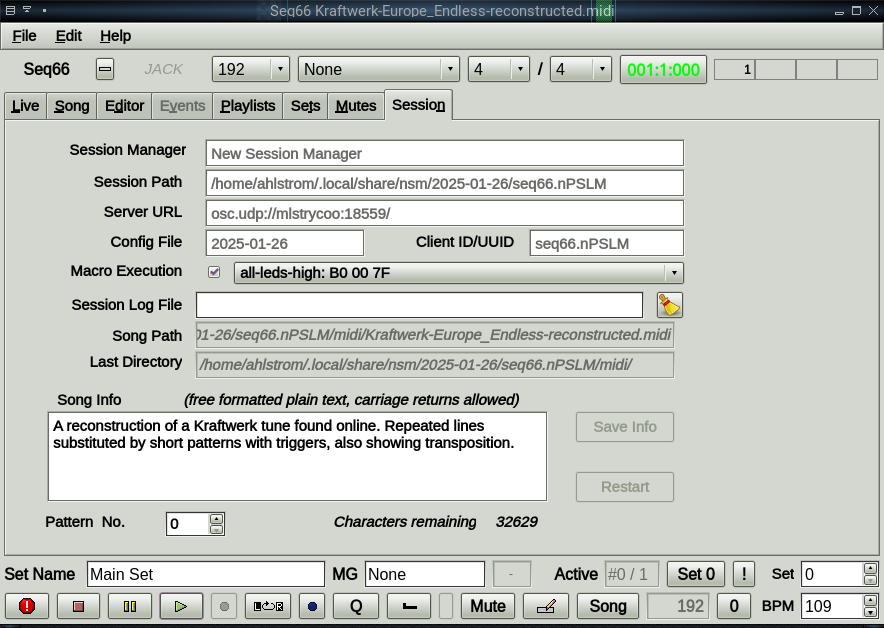
\includegraphics[scale=0.65]{tabs/session/session-song-info.png}
   \caption*{Session Tab with Song Info}
\end{figure}

   \index{sessions!ui}
   This section describes the \textsl{Session} tab in the main
   \textsl{Seq66} window.  This tab displays mostly informative and
   \textsl{read-only} information (except for the name of the log file
   and the editable song-info pane).
   It displays the following bits of information that \textsl{Seq66} has
   received from \textsl{NSM} via the \texttt{nmsd} daemon:

   \begin{itemize}
      \item \textbf{Session Manager}. The name of the session manager as
         sent by the session manager.
      \item \textbf{Session path}.
         The root ("home") configuration directory of the session.
         All data goes into this directory.
         The name of the "home" directory is of the form
         \texttt{HOME/nsmroot/sessionname/uniqueid}.
         \texttt{HOME} is the usual UNIX home directory for the user.
         "nsmroot" depends on which version of the New/NSM session manager is
         used.
         \index{session!non}
         For the original \textsl{NSM}, this directory is \texttt{NSM Sessions}.
         \index{session!new}
         For the \textsl{New Session Manager}, this directory is
         \texttt{.local/share/nsm}.
         The session name is provided by the user when creating the
         session.
         The unique ID is generated by the non/new session manager.
         If not running in a session,
         the active configuration directory is shown.
      \item \textbf{Server URL}.
         The session's \textbf{OSC URL}, which includes the port number.
         Generally, the port number is selected at run-time, but it is also
         possible to configure \textsl{NSM} to use a specific port number.
      \item \textbf{Config File}.
         This is either the display name for the session, the
         sub-directory that contains the session configuration, or
         the base name of the main configuration file,
         such as \texttt{qseq66.rc}.
      \item The generated \textbf{client ID/UUID} for the session.
      \item \textbf{Macro Execution}.
         This drop-down contains all of the named MIDI macros
         defined in the 'ctrl' file's
         \texttt{[macro-control-out]} section.
         By selecting one, it is automatically sent out via the
         \texttt{[output-buss]} port defined in the 'ctrl' file.
         The "startup" and "shutdown" macros, if defined,
         are sent automatically. "Startup" is useful to put
         a MIDI controller into the proper mode for controlling and displaying
         information in \textsl{Seq66}, and "shutdown" can return the controller
         to its normal operating mode.
      \item \textbf{Session Log File}.
         The editable name of the log file
         to which to redirect warning
         and error messages during the action of \textsl{qseq66}.
         Normally, the text is shown in the console window (when running in a
         console window). This name is only a base-name (e.g.
         \texttt{seq66.log}); it is always stored in the "home" configuration
         directory, whether normal or the NSM session directory.
      \item \textbf{Song Path}.
         Holds the full file-specification of the currently-loaded MIDI
         file.
      \item \textbf{Last Directory}.
         Shows the directory from where the last MIDI file was loaded.
      \item \textbf{Restart}.
         \index{restart!manual}
         After editing some of the preferences in the \textbf{Edit / Preferences}
         dialog, one can (later)
         visit this tab and press this button to essentially
         restart \textsl{Seq66}, reloading the new configuration.
         Be careful!
      \item \textbf{Song Info}.
         \index{song!info}
         \index{meta text}
         This item is a plaintext edit-control that allows the viewing and
         editing of "song info".
         The song info is merely the first Meta Text event, if any,
         found in pattern 0.
         The pattern number can be changed if desired, to show text in other
         patterns.
         This field can be edited with information such as date, composer,
         playback notes, etc. up to about 32000 ASCII characters.
         Extended ASCII characters are encoded as three hexadecimal
         bytes: \texttt{$\backslash$xx}.
      \item \textbf{Pattern No}.
         This spin box allows for viewing and editing the text
         in a selected pattern.
      \item \textbf{Save Info}.
         When clicked, the meta text is copied to the selected pattern,
         thus modifying the file, which can then be saved.
         \index{karaoke}
         For tracks (such as a karaoke lyric track) with many text events,
         they are all shown, separated by semi-colons.
         Don't try to edit karaoke data, except in the \textsl{Event Editor}.
         A simple description for each pattern is fine to edit.
         An example of a karaoke song is found in the \texttt{contrib/midi}
         directory:
         \texttt{Carpet\_of\_the\_Sun\_karaoke\_meta\_text.mid}.
      \item \textbf{Restart}.
         When in NSM, this button is enabled when a restartable change is
         made here.
   \end{itemize}

   Note that there are many implementations of NSM clients:
   \textsl{Agordejo} \cite{agordejo},
   \textsl{RaySession} \cite{raysession},
   and the
   \textsl{New/Non Session Manager} \cite{nsm}
   with the JACK project's \texttt{nsm-legacy-gui}.

\subsubsection{Seq66 Session Management / NSM / File Menu}
\label{subsubsec:sessions_file_menu}

   The author of \textsl{NSM} has provided documentation for session-management
   which provides very strict instructions on how an application must behave
   under session management.  \textsl{Seq66} tries very hard to stick to these
   instructions.  One major adjustment an application must make is to adhere to
   the "File menu" guidelines.

\begin{figure}[H]
   \centering 
   \includegraphics[scale=0.65]{tabs/session/nsm-qseq66-menus-2.png}
   \caption*{File Menu Under NSM, Composite View}
\end{figure}

   Not (yet) shown in the figure are the \textbf{Project Configuration}
   options for import and export.
   (See \sectionref{subsec:menu_file}.)

   This has been changed for 0.98.6; the \textbf{Quit} menu entry becomes
   \textbf{Hide}, as per the NSM protocol.  Also have fixed a bug that disables
   the load-most-recent option under NSM.
   We will update the figure above eventually.
   The following items describe the menu entries.

   \begin{itemize}
      \item \textbf{New MIDI File}.
         This function prompts for the name of a
         new MIDI file and clears the current MIDI file.  The file-name must not
         include a full-path to the file.  The path is hardwired by the
         session.  A relative path can be included.  This name is needed
         because there is no "Save As" option when running in an \textsl{NSM}
         session.
      \item \textbf{Import / Project Configuration...}
         Imports a whole project configuration into the current NSM session.
         This functionality used to be automatic (importing the "home"
         configuration), but it is better left to the user to do.
         \index{restart!automatic}
         However, the restart of \textsl{Seq66} after this operation is
         automatic.  Be careful!
      \item \textbf{Import / MIDI to Current Set...}
         This action works the same as in normal mode.
         This item allows the user to grab a MIDI file from anywhere and import
         it into the current set.
         The default directory that comes up in the
         prompt is the "last-used directory" from the session 'rc' file.
      \item \textbf{Import / Playlist...}
         This action works the same as in normal mode.
         The destination is the NSM session directory.
         \index{restart!automatic}
         Once the playlist is imported,
         \textsl{Seq66} is automatically \textsl{\textbf{restarted}}
         in order to load the playlist.
         Be careful!
      \item \textbf{Import / Import into Session...}
         Prompts the user for a MIDI file to
         be imported (copied) into the current session.  The path to the file
         is then adjusted to use the \textsl{NSM} \texttt{midi} subdirectory.
      \item \textbf{Export / Song...}
         Allows exporting the current song as a stock MIDI file, using the
         performance information (triggers) to write the MIDI data as it would
         be played in "song" mode.
         The default directory that comes up in the
         prompt is the "last-used directory" from the session 'rc' file.
      \item \textbf{Export / MIDI Only...}
         Allows exporting the current song as a stock MIDI file.
         The "proprietary" SeqSpec data is \textsl{not} written.
         The default directory that comes up in the
         prompt is the "last-used directory" from the session 'rc' file.
      \item \textbf{Export / SMF 0...}
         This action works the same as in normal mode.
         It converts the destination file to SMF 0 format.
      \item \textbf{Hide}.
         This menu item replaces the \textbf{Quit} item.
         It hides the main window and tells NSM about it.
   \end{itemize}

   At some point we would like to present a small tutorial showing a session
   under \textsl{JACK}.
   Also note that NSM can invoke or kill applications via
   \textsl{signals}, as explained in 
   \sectionref{subsec:sessions_signals}.

\subsubsection{Seq66 Session Management / NSM / Debugging}
\label{subsubsec:sessions_debugging}

   This section is oriented towards advanced users who found a problem running
   \textsl{Seq66} and want to track it down themselves.  The issue is that we
   need to start the application under the debugger, or start it under NSM and
   somehow attach to \textsl{Seq66} before it starts running.  Another issue is
   that we have found that, at least on the same host, an NSM session
   \textsl{must} be open before \textsl{Seq66} can attach to it, even if the
   correct \texttt{NSM\_URL} is provided.
   So we have to open a session, get the proper URL, configure it in the 'usr'
   file, and then start \textsl{Seq66} under the debugger.
   Here are the steps:

   \begin{enumerate}
      \item Start \textsl{non-session-manager} from a command-line console.
         Write down the URL that it advertises.
      \item Prepare a session for the executable as per earlier instructions.
         Once \texttt{qseq66} starts, immediately exit it, and leave the session
         open.
      \item Open the proper 'usr' file (usually \texttt{qseq66.usr}) in a 
         text editor.  Set variable "session = nsm", and set the variable "url"
         to the value that was advertised.
      \item Now start \texttt{qseq66} in a debugger.
      \item Set a breakpoint in \texttt{clinsmanager::detect\_session()}.
   \end{enumerate}
   
   Now you can step through and see where NSM and Seq66 are getting mixed up.
   Also check the session directory afterward to make the configuration
   (and any MIDI files) are in good shape.

\subsection{Seq66 Session Management / LASH}
\label{subsec:sessions_lash}

   \index{sessions!lash}
   LASH support has been removed.  Use the \textsl{NSM Session Manager} or
   the \textsl{JACK Session Manager}.

\subsection{Seq66 Session Management / sessions.rc}
\label{subsec:sessions_sessions_rc}

   \texttt{Seq66} also supports a more simplistic type of "session",
   where a whole different set of configuration files can be selected.

   One can use the \texttt{-{}-home} and \texttt{-{}-config} options
   to specify alternate locations and names for the configuration files.
   However, if one has a number of configurations
   (e.g. for different sets of equipment. playlists,
   style-sheets, and palettes),
   it's tedious to type these options.
   The \texttt{sessions.rc} file provides a way to set up a
   number of configurations and select one with one option.
   It is always located in the default
   "home" directory, but can refer to directories anywhere. It can also
   specify a different MIDI client-name
   (option \texttt{-{}-client-name})
   and log-file
   (option \texttt{-{}-option log=filename}).

   The user must manually text-edit the sessions.rc to specify tag
   sections like the following:

   \begin{verbatim}
       [test]
       home = "~/.config/seq66/test/"
       config = "test66"
       client-name = "test66"
       log = "test66.log"
   \end{verbatim}

   \index{-{}-session-tag}
   \index{session-tag}
   This section is accessed using the \texttt{-S} or
   \texttt{-{}-session-tag} option, as shown here:

   \begin{verbatim}
       $ qseq66 --session-tag test
       $ qseq66 -S test
   \end{verbatim}

   If this is the first time this command has been run, the
   home directory is created.
   (At present, though, the initial configuration files are not
   created until \textsl{Seq66} exits.)
   \textsl{Seq66} runs with a MIDI client-name of
   \texttt{test66}.
   The base-name of each configuration file
   is \texttt{test66} (so we have, for example, \texttt{test66.rc}).
   The log file will be
   \texttt{~/.config/seq66/test/test66.log}.
   (If no log file is wanted, then set it to \texttt{""} later.)

   At the end of the run, all of the configuration files are
   saved in 
   \texttt{~/.config/seq66/test/}.
   These can be edited to suit the "test" configuration.
   The setup can also be created via
   \textbf{File / Export / Project Configuration},
   and then be added to \texttt{sessions.rc}.

   The next time 
   \texttt{qseq66 -{}-session-tag test}
   is run, the test configuration is loaded and used.

   If the specified session tag does not exist in \texttt{sessions.rc},
   then a message is shown; the user should exit \textbf{Seq66} immediately
   and fix \texttt{sessions.rc}.

   Note that the \texttt{log} option overrides the log-file setting
   present in the 'usr' file. Use \texttt{log = ""} to see console output.

   Lastly, an environment variable can be used to set a session-tag that
   will be used for quite awhile.
   It can be exported in a \texttt{bash} script, a profile,
   or set on the command-line (which is more difficult that using the
   option):
   \index{SEQ66\_SESSION\_TAG}

   \begin{verbatim}
       $ SEQ66_SESSION_TAG="test" qseq66
   \end{verbatim}


%-------------------------------------------------------------------------------
% vim: ts=3 sw=3 et ft=tex
%-------------------------------------------------------------------------------


% Import/Export

%-------------------------------------------------------------------------------
% midi_export
%-------------------------------------------------------------------------------
%
% \file        midi_export.tex
% \library     Documents
% \author      Chris Ahlstrom
% \date        2018-10-20
% \update      2025-05-26
% \version     $Revision$
% \license     $XPC_GPL_LICENSE$
%
%     This section discusses the details of the import/export functionality.
%
%-------------------------------------------------------------------------------

\section{MIDI Import/Export}
\label{sec:midi_import_export}

   This section explains the details of the MIDI import and export
   functionality, accessed by the main menu as noted in sections
   \ref{subsubsec:menu_file_import},
   \ref{subsubsec:menu_file_export_project},
   \ref{subsubsec:menu_file_export_song_as_midi}, and
   \ref{subsubsec:menu_file_export_midi_only}, on page
   \pageref{subsubsec:menu_file_import}.

\subsection{File / Import Menu}
\label{subsec:midi_export_file_import_menu}

   The actions for importing files have been move to the new
   \textbf{File / Import} menu in order to keep from cluttering the
   ever-expanding file menu.

\subsubsection{Import Project Configuration}
\label{subsubsec:midi_export_file_import_project}

   This operation allows one to import all of the \texttt{qseq66.*}
   configuration files from a given directory into the current run of
   \textsl{Seq66}.
   It is most useful when
   importing a configuration into a new \textsl{NSM} session.
   \index{restart!automatic}
   Once the files are copied, \textsl{Seq66} is automatically restarted,
   in order to load the new configuration.  Be careful!

   Note that the names of the configuration files being impported should
   match the canonical names.  That is, the base names should all be
   \texttt{qseq66} (or \texttt{qpseq66} for \textsl{Windows}.)

   If importing into an NSM session, one must use the NSM user-interface
   (\textsl{agordejo}, \textsl{RaySession}, or \textsl{nsm-legacy-gui}
   to \textsl{Stop} and then \textsl{Start} \textsl{Seq66}.

\subsubsection{Import MIDI Into Current Set}
\label{subsubsec:midi_export_file_import}

   The \textbf{File / Import / Import to Current Set} menu entry imports an SMF 0
   or SMF 1 MIDI file as one or more patterns, one pattern per track, and
   imports them into the currently-active set.
   Even long tracks, that aren't short loops, are imported.
   The difference from \textbf{File / Open} is that the destination screen-set
   (bank) for the import can be specified, and the existing data in the
   already-loaded MIDI file is preserved.
   If the imported file is a
   \textsl{Seq66} MIDI file, it's proprietary sections will
   \textsl{not} be imported, in order to preserve the performance setup.
   The \textbf{Import} dialog is similar to the \textbf{Open} dialog.

   When imported, each track, whether music or information,
   is entered into its own loop/pattern box (slot).
   The import operation can handle reasonably complex files.
   When the file is imported, the sequence number for each track is
   adjusted to put the track into the desired screen-set.
   The import can place the imported data into any of the 32 available
   screen-sets.  Quite large songs can be built by importing patterns.

   Import also handles SMF 0 MIDI files.  It parcels out the SMF 0 data
   into sequences/patterns for each of the 16 MIDI channels.  It also puts
   all of the MIDI data into the 17th pattern (pattern 16), in case it is
   needed.  Note that this slot is used no matter which screen-set one imports
   the file into.  Bug, or feature?
   Also note that, since the file information has been modified by the import,
   the user will be prompted to save the file when exiting \textsl{Seq66}.
   Finally, conversion to SMF 1 for SMF 0 files can be disabled using the
   'usr' option \texttt{[user-midi-settings] convert-to-smf-1}.

\subsubsection{Import Playlist}
\label{subsubsec:midi_export_file_import_playlist}

   This operation allows one to copy a playlist and its MIDI files.
   from one directory to another.  It is most useful when
   importing a configuration into a new \textsl{NSM} session.
   Here are the steps it performs:

   \begin{itemize}
      \item Copies the selected playlist file (e.g. \texttt{liveset.playlist})
         into the current configuration directory.
         This directory is one of the following:
         \begin{itemize}
            \item The default "home" directory,
               \texttt{\textasciitilde/.config/seq66}.
            \item A "home" directory specified by the \texttt{--home} option.
            \item The session directory created by \textsl{NSM}.
         \end{itemize}
         For discussion, this directory is called "HOME" or "home".
      \item In HOME, creates a directory called (for example)
         \texttt{playlist/liveset},
         where "liveset" is the base part of the playlist name, as in
         \texttt{liveset.playlist}.
      \item The playlist is opened, parsed, and all of the MIDI tunes specified
         in that file are copied into the new playlist directory, preserving
         the directory directory structure of the original playlist.
      \item The 'rc' file is modified to specify the new playlist,
         specify that it is \texttt{active},
         to specify the new \texttt{base-directory} for all of the tunes,
         and to specify that the playlist will be saved at exit.
      \item Lastly, if not running within NSM, \textsl{Seq66} will be
         \index{restart!automatic}
         \textsl{\textbf{restarted}} automatically to load the new,
         active playlist.
         Within NSM, the user must stop and restart \textsl{Seq66}
         manually in the NSM user-interface.
         Be careful!
   \end{itemize}

\subsection{File / Export Menu}
\label{subsec:midi_export_file_export_menu}

   The actions for exporting files have been moved to the
   \textbf{File / Export} menu in order to keep from cluttering the
   ever-expanding file menu.

   An important point to note is the pattern/channel behavior inherited
   from \textsl{Seq24}.
   When a pattern has a channel specified, all MIDI channel events
   (e.g. Note On/Off) are stamped with that channel when exported.
   This applies to exports to plain MIDI files, song exports, and
   exports to the SMF 0 format.

   If one wants to preserve the channel number for all events in
   a pattern, then one should set the channel to the \textbf{Free}
   value.  See \sectionref{subsec:pattern_editor_first_row}, the section on
   \textbf{Channel Selection}.

   Also note that exporting a song or an SMF 0 file require that the song
   be exportable (see the next section).
   Exporting to a regular MIDI does not have this requirement.

\subsubsection{Export Project Configuration}
\label{subsubsec:midi_export_configuration_export}

   This option allows the various \texttt{qseq66.*} configuration
   files to be copied to another directory.
   This feature is useful for creating an alternate configuration or
   for backing up the current configuration.

   At the present time, any files specified in a play-list are
   \textsl{not} copied.

\subsubsection{Export Song}
\label{subsubsec:midi_export_song_export}

   Thanks to \textsl{Seq32}, exporting song performances (see the
   \textbf{Song Editor}) to standard MIDI format has been added.
   The \textbf{File / Export / Export Song} operation modifies the song in the
   following ways:

   \begin{itemize}
      \item Only tracks (sequences, loops, or patterns)
         \index{exportable}
         that are "exportable" are written.  To be exportable, a
         track must have triggers
         (see \sectionref{subsubsec:concepts_terms_performance})
         present in the \textbf{Song Editor}.
         Also \textsl{in the song editor}, it must \textsl{not be muted}.
      \item Each trigger generates the events, including repeats,
         offset-play of the events, and transposition.
         If there is a gap in the layout
         (e.g. due to an \textbf{Expand} operation in the
         \textbf{Song Editor}),
         then the corresponding gap in the events is exported.
         The result is a track that reconstructs the original
         playback/performance layout of that pattern.
         The events themselves are sufficient to play the performance exactly
         in any MIDI sequencer.
         The triggers are useful for further editing of the song/performance,
         so they are preserved in the triggers \textsl{SeqSpec} section, but
         they cover the whole song.
         The process of consolidating the trigger data is called
         "flattening".
      \item Empty pattern slots between tracks are removed.
      \item No matter what set the original track was in, it ends up in the
         first set; sets are consolidated.
      \item Other additions, such as time signature and tempo meta events, are
         written in the same manner as for a normal \textbf{File / Save}
         operation.
   \end{itemize}

   The \textbf{Export} dialog is similar to the \textbf{Open} dialog;
   one will likely want to change the name of the file so as
   not to overwrite it.
   If there are no exportable tracks, the following message is shown:

\begin{figure}[H]
   \centering 
   \includegraphics[scale=0.65]{main-menu/file/light-menu-file-song-unexportable.png}
   \caption{MIDI File Unexportable}
   \label{fig:midi_export_file_unexportable}
\end{figure}

   Once the file is exported, reopen it to see the results of the export.
   The following figure shows a before and after picture of the export, as
   seen in the song editor.

\begin{figure}[H]
   \centering 
   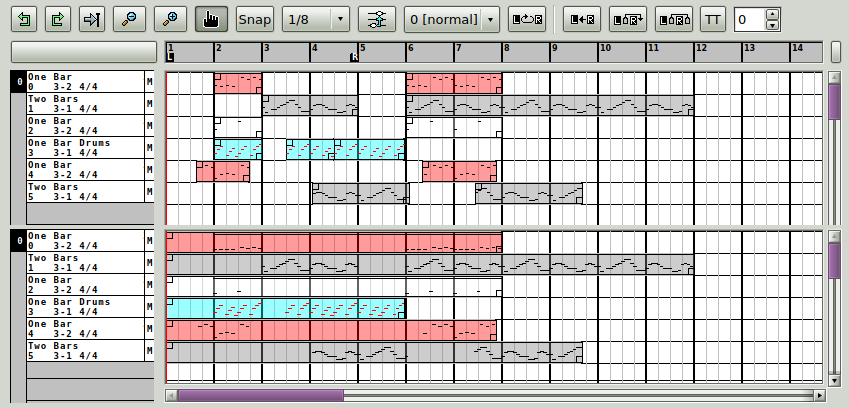
\includegraphics[scale=0.75]{song-editor/song-layout-sample-2.png}
   \caption{MIDI File Layout Before/After Export}
   \label{fig:midi_export_file_before_after}
\end{figure}
   
   The gaps in layouts in the song/performance data are reflected in the
   consolidated triggers.
   Here is the before/after triggers for pattern \#0, which was
   layed out with \textbf{Record Snap} \textsl{on}:

   \begin{verbatim}
       BEFORE                              AFTER
      Sequence #0 'One Bar'               Sequence #0 'One Bar'
      Length (ticks): 768                 Length (ticks): 5375
      trigger: 768 to 1535 at 768         trigger: 0 to 5375 at 5375
      trigger: 3840 to 5375 at 768        
   \end{verbatim}

   Note that 768, at PPQN = 192, is 4 beats (1 measure), while 5375 is 28
   beats (7 measures).
   For each of these triggers, the first number is the start of the trigger in
   PPQNs, the second is the end of the triger, and the third, called the
   "offset", is actually the length of the pattern.
   Note how the "AFTER"
   trigger consolidates the "BEFORE" triggers, starts at time 0, extends to
   the end of the last trigger, and has a length equal to the end of the
   trigger.

   Now here is the before/after triggers for pattern \#5, which was
   layed out with \textbf{Record Snap} \textsl{off}:

   \begin{verbatim}
       BEFORE                              AFTER
      Sequence #5 'Two Bars'              Sequence #5 'Two Bars'
      Length (ticks): 1536                Length (ticks): 6911
      trigger: 2344 to 3879 at 1536       trigger: 0 to 6655 at 6911
      trigger: 4944 to 6655 at 0
   \end{verbatim}

   6655 is a little over 34.5 beats, which is what the bottom grey trigger
   shows.
   6911 is almost 36 beats (9 measures).  Something to figure out.

\subsubsection{Export MIDI Only}
\label{subsubsec:midi_export_file_export_midi_only}

   Sometimes it might be useful to export only the non-sequencer-specific
   (non-SeqSpec) data from a \textsl{Seq66} song.
   For example, some buggy sequencers
   (hello \textsl{Windows Media Player})
   might balk at some SeqSpec item in the song, and refuse to load the MIDI
   file.
   For such cases,
   the \textbf{File / Export / Export MIDI Only} menu
   item writes a file that does not contain
   the SeqSpec data for each track, and does not include all the SeqSpec data
   (such as mute groups) that is normally written to the end of the
   \textsl{Seq66} MIDI file.

\subsubsection{Export SMF 0}
\label{subsubsec:midi_export_file_export_smf_0}

   In some cases it might be useful to convert a \textsl{Seq66} MIDI file to a
   single-track SMF 0 file.
   As with exporting to a song
   (see \sectionref{subsubsec:midi_export_song_export}),
   the tracks to be exported (combined into a single track) must be unmuted.
   \textsl{However}, it is not worthwhile to export a MIDI tune
   that is in Song mode, unless all the patterns are the same length.
   To export in Song mode, first use Song export (see
   \sectionref{subsubsec:midi_export_song_export}), then export the modified
   tune to SMF 0.

   The \textbf{File / Export / Export SMF 0 } menu
   action removes all the existing tracks and merges them into track 0.
   The original tune can be opened again, if desired.

%-------------------------------------------------------------------------------
% vim: ts=3 sw=3 et ft=tex
%-------------------------------------------------------------------------------


% Recording

%-------------------------------------------------------------------------------
% seq66 recording
%-------------------------------------------------------------------------------
%
% \file        seq66 recording.tex
% \library     Documents
% \author      Chris Ahlstrom
% \date        2023-11-25
% \update      2025-05-30
% \version     $Revision$
% \license     $XPC_GPL_LICENSE$
%
%     Provides a discussion of the MIDI GUI recording that Seq66
%     supports.
%
%-------------------------------------------------------------------------------

\section{Seq66 Recording In Depth}
\label{sec:recording}

   Recording in \textsl{Seq66} has been greatly enhanced.
   Multiple patterns can be recorded at once, with events
   routed to particular patterns based on the buss number the event came
   in on, or its channel number.
   Additional ways to toggle recording have been added.
   Additional recording alterations have been added, such as on-the-fly note
   mapping.
   It can get a bit complex to keep track of, hence this section,
   which walks the user through some scenarios.

   Before getting started, note that recording also
   can be done during count-in via the metronome feature.
   See \sectionref{subsection:edit_preferences_metronome}.

\subsection{Recording Scenarios}
\label{sec:recording_scenarios}

   The following recording scenarios are available:

   \begin{itemize}
      \item \textbf{Standard Recording}.
         This provides the normal method of recording. Open a pattern in a
         window and enable recording, or right-click on its live-grid
         slot and enable recording..
         The last slot selected for recording receives the events.
         Events are received from all enabled MIDI input ports.
         In this mode the record-button at the bottom of the main window
         is red.
         The slot popup-menu does not provide for setting an input buss
         in this mode.
      \item \textbf{Record-by-Bus}.
         In this mode, any pattern that specifies a specific input buss
         can be enabled for recording.
         Incoming events are routed to the first pattern that has an input
         buss matching the buss on which the event was recorded.
         In this mode the record-button at the bottom of the main window
         is green.
         To designate a recording buss, first go to
         \textbf{Edit / Preferences / MIDI Input} and enable
         \textbf{Record into patterns by bus}.
         Then right-click on the pattern and select an
         \textbf{Input bus}. (This popup menu entry only appears when
         record-by-bus is active.)
      \item \textbf{Record-by-Channel}.
         In this mode, one enables recording in patterns numbered from 0 to 15
         (channels 1 to 16) with output channels set from 0 to 15.
         Incoming events are analyze for their channel and are recording into
         the corresponding pattern number.
         In this mode the record-button at the bottom of the main window
         is yellow.
   \end{itemize}

   The "Record-by" options above are mutually exclusive.

\subsubsection{Standard Recording}
\label{subsubsec:recording_standard_recording}

   Standard recording allows the enabling of recording in a single pattern.
   It \textsl{requires} that the other two modes be turned off.
   Once a pattern is set to record, no other pattern can be set to record until
   the original pattern is set to not record.
   The single recording pattern gets all events from any MIDI
   input that is enabled.

   In standard recording there a many ways to enable recording into
   a pattern.

   \begin{itemize}
      \item Open the pattern editor in a window or tab or click on the
         pattern slot to record, then click the red record
         button at the bottom of the pattern editor.
         The pattern will also
         show a red circle to indicate that recording has been enabled.
      \item Right-click on the desired pattern in the grid and select
         \textbf{Record toggle} from the menu.
      \item Touch a pattern or click its hot key, then
         click the red record button at the bottom of the main window.
      \item Select the \textbf{RECORD} grid mode, then select a pattern.
         To change the selected slot, click on the red record button
         to disable recording, then click on the desired slot.
         Recording is active on that slot.
         (This option is more useful in the other recording scenarios.)
   \end{itemize}

   Again, remember that, with standard recording, only one pattern can
   accept events.
   Also note that this mode should be used if one
   expects to record SysEx events, which have no channel.

\subsubsection{Route-Input-By-Buss}
\label{subsubsec:recording_route_by_buss}

   \index{record!by buss}
   Route-input-by-buss (also known as record-by-buss)
   is enabled whenever a pattern in a song specifies an
   input buss \textsl{and}
   \textbf{Edit / Preferences / MIDI Input / Record into patterns by
   bus} is checked. It is an 'rc' file option.
   If it is enabled, it supercedes the
   \textbf{record-by-channel} option and
   disables that standard recording mode described above.

   When route-by-bus is enabled, an internal container is populated with
   all the patterns in the current play-set that specify an input buss.
   This container is rebuilt when a sequence is added or removed.
   It is stored in the \texttt{c\_midiinbus} SeqSpec in the song.

   If route-by-bus is enabled, a sequence with an input bus that matches the
   buss associated with the incoming event is looked up, and input is
   streamed to it.

   In this scenario, multiple patterns can be enabled for recording,
   and output from multiple input ports are routed appropriately.

   For the green record button to be enabled, at least one pattern
   must specify an input bus.
   Clicking on the green record button at the bottom of the main window
   will turn on recording for \textsl{all}
   patterns that specify an input buss.

\subsubsection{Record-By-Channel}
\label{subsubsec:recording_record_by_channel}

   Record-by-channel can be enabled in
   \textbf{Edit / Preferences / MIDI Input / Record into patterns by
   channel}, which is an 'rc' file option.

   It works by routing events to the first pattern that has specified an 
   output (not input) channel that matches the channel (if applicable) of
   the incoming MIDI event.
   The patterns applicable are entered into a list of patterns with specified
   output channels.

   \textbf{IMPORTANT}:
   In order for a channel to be recorded, it's corresponding pattern
   must exist. Hence,
   for convenience, there is a MIDI file installed, called
   \textbf{16-blank-patterns}, which specifies all the output channels.
   It can be copied and used for the first recording from a device
   playing on multiple channels, or from multiple devices, each playing
   on a different channel.

   Clicking on the yellow record button at the bottom of the main window
   will turn on recording for \textsl{all}
   patterns, except for patterns that specify "Free" (i.e. no forced channel).

   Note that the route-by-buss option, described above, supercedes this
   option.

\subsection{Recording Modes}
\label{sec:recording_modes}

   Recording can also transform (alter) the incoming events.

   \begin{itemize}
      \item \textbf{Tighten}.
         Partial quantization to the current snap value.
      \item \textbf{Quantize}.
         Full quantization to the current snap value.
      \item \textbf{Note-map}.
         If a 'drums' file is active, then notes are changed
         in note-value according to that file.
         This is most useful for drums, but other effects are possible.
   \end{itemize}

   These transformations can also be done after recording.

\subsection{Seq66-to-Seq66 Recording}
\label{sec:recording_seq_to_seq}

   This section describes a way to have one instance of \textsl{Seq66}
   (\texttt{qseq66}) interact with another.
   The first \textsl{Seq66} to start runs with a different client name
   (optional) and a different 'rc' file name (to not affect the normal
   configuration of \textsl{Seq66}).
   The first \textsl{Seq66} runs with virtual ports; the second
   \textsl{Seq66} runs normally and can auto-connect to these
   ports.

   The first instance:

   Run and exit to create the configuration files, then run with
   the "virtual" option; the first number is the number of output ports
   to make, and the second is the number of input ports to make.

   \begin{verbatim}
       $ qseq66 --client first66 --rc first66
       $ qseq66 --client first66 --rc first66 --option virtual=2,2
   \end{verbatim}

   In the \textbf{MIDI Clock} tab should be "first66:midi out 0" and
   "first66:midi out 1".
   In the \textbf{MIDI Input} tab should be "first66:midi in 0" and
   "first66:midi in 1".
   Among the ports shown, along with plugged in hardware, are:

   \begin{verbatim}
      $ aplaymidi -l
       Port    Client name                      Port name
       44:0    MPK mini Play mk3                MPK mini Play mk3 MIDI 1
      128:0    first66                          midi in 0
      128:1    first66                          midi in 1
      ahlstrom@mlstrycoo ~/Home/ca/mls/git/seq66
      $ arecordmidi -l
       Port    Client name                      Port name
       44:0    MPK mini Play mk3                MPK mini Play mk3 MIDI 1
      128:2    first66                          midi out 0
      128:3    first66                          midi out 1
   \end{verbatim}

   Leave this instance running, and run a plain \texttt{qseq66} command.
   It should show the "first66" output (clocks) and input ports.

   One should now be able to pass MIDI events between the two instances.

% VERIFY this at some point.

%-------------------------------------------------------------------------------
% vim: ts=3 sw=3 et ft=tex
%-------------------------------------------------------------------------------


% Configuration files are now consolidated into one file

%-------------------------------------------------------------------------------
% configuration
%-------------------------------------------------------------------------------
%
% \file        configuration.tex
% \library     Documents
% \author      Chris Ahlstrom
% \date        2021-01-18
% \update      2025-06-09
% \version     $Revision$
% \license     $XPC_GPL_LICENSE$
%
%     Provides the configuration information.
%
%-------------------------------------------------------------------------------

\section{Seq66 Configuration}
\label{sec:configuration}

   \textsl{Seq66} configuration has become more elaborate with time, with more
   configuration files.
   Configuration items are well documented in the
   \textsl{Seq66} "man" page and in the configuration files.
   Therefore, this new discussion will merely summarize the options and
   go into a few details about the configuration files.
   Here are the topics to discuss:

   \begin{itemize}
      \item \textbf{Command-line Options}. Useful with desktop shortcuts.
      \item \textbf{'rc' File}. Mostly I/O port options, JACK options, recent
         files.  Also now specifies other files to be used.
      \item \textbf{'usr' File}. Local names for busses and instruments,
         user-interface settings, sessions... Some options that fit either the
         GUI or the command-line application could be moved to the 'rc' file.
      \item \textbf{'ctrl' File}. The keystroke and MIDI control settings have
         been moved to a separate file for flexibility.
      \item \textbf{'mutes' File} The mute-groups settings have
         been moved to a separate file for flexibility.
      \item \textbf{'drums' File}.  This file supports remapping percussion
         notes from older drum machines to General MIDI.
      \item \textbf{'playlist' File}. This new file specifies a file that
         contains one or more playlists and MIDI controls for them.
      \item \textbf{'palette' File}. This new file allows replacing the default
         piano-roll, time, data, and events drawing to be tailored separately
         from the Qt theme.
      \item \textbf{'qss' File}.  Qt style-sheets can now tailor the appearance
         of Qt theme-drawn elements
         (e.g. the pattern-grid buttons and text controls).
   \end{itemize}

   After the first run and exit of \textsl{Seq66},
   it generates a set of default configration files in the default
   \textsl{configuration} directory:

   \begin{verbatim}
      /home/user/.config/seq66/qseq66.rc
      /home/user/.config/seq66/qseq66.usr
      /home/user/.config/seq66/qseq66.ctrl
      /home/user/.config/seq66/qseq66.mutes
      /home/user/.config/seq66/qseq66.drums
      /home/user/.config/seq66/qseq66.playlist
      /home/user/.config/seq66/qseq66.palette
   \end{verbatim}

   The palette file is not automatically generated.  It can be saved from the
   \textbf{Edit / Preferences / Display} tab.
   There are also samples installed in the \texttt{data/samples}
   directory.
   The style-sheet file can be specified in the 'rc' file's
   \texttt{[style-sheet-file]} section.
   There are also some 'keymap' files.  They are not yet used, but may become a
   feature of \textsl{Seq66} in the future.
   For \textsl{Microsoft Windows}, the default base name of the files is
   \texttt{qpseq66}, and the default configuration directory is

   \begin{verbatim}
        C:/Users/user/AppData/Local/seq66/
   \end{verbatim}

   When running \textsl{Seq66} from the \textsl{Non Session Manager}
   (Linux-only, see \sectionref{sec:sessions}),
   the configuration directory is automatically set to something like

   \begin{verbatim}
      /home/user/NSM Sessions/MySession/seq66.nRSIQ/config
   \end{verbatim}

   There is no palette file by default, but the user can create one.
   The color palettes are discussed in \sectionref{sec:palettes}.
   Other files contain the the data for remote MIDI control, computer keyboard
   control, MIDI clock, JACK transport, and a many other settings.
   Some of the settings can be modified in the \textbf{Edit / Preferences}
   dialog, or overridden from the command line.

   \textsl{Seq66} overwrites the most of these files upon exiting.
   One must therefore quit \textsl{Seq66} before making
   manual modifications to these files.

\subsection{Configuration File Commonalities}
\label{subsec:configuration_file_commonalities}

   All of the \textsl{Seq66} configuration files have the following in common:

   \begin{itemize}
      \item \textbf{[Seq66] Section}
      \item \textbf{[comments] Section}
      \item \textbf{Numeric Settings}
      \item \textbf{Boolean Settings}
      \item \textbf{Variables}
      \item \textbf{Stanzas}
   \end{itemize}

   Generally, each configuration file has its own specific set
   of sections, each section-name being enclosed in square brackets in a very
   strict format:  No spaces inside the square brackets.  Sections are looked up
   by this name, including the square brackets, and the name must be exact.

\subsubsection{[Seq66] Section}
\label{subsec:configuration_common_seq66_section}

   This section is informational.  At a minimum, it holds two
   variables:

   \begin{itemize}
      \item \texttt{config-type}.  This value indicates the type of the file,
      such as "ctrl" or 'rc'.
      \item \texttt{version}.  This value indicates the version of the file.
      It is used in some cases when we have added a feature to the
      configuration file that cannot be automatically handled.
      When the internal version number of the file is incremented,
      it can be used to make adjustments for changes in configuration when
      reading older versions of files.
   \end{itemize}

   This section may also contain additional "global"
   variables specific to a given \texttt{config-type}.

\subsubsection{[comments] Section}
\label{subsec:configuration_common_comments_section}

   The "comments" section is also informational, but the user can edit this
   section to include information describing the purpose of the file.  For
   example, a 'ctrl' file for a \textsl{Novation Launchpad}
   (see \sectionref{sec:launchpad_mini})
   might describe the
   purpose of this file.  The comments stop at the first blank (not even spaces)
   line.  To skip a line in the comment, put a single space character on the
   blank line.

\subsubsection{Numeric Settings}
\label{subsec:configuration_common_numeric_settings}

   Numeric settings consist of a line containing one or more numbers, usually
   preceded by an explanatory comment, and followed by a standard script
   comment.

   \begin{verbatim}
      output-port-count = 8   # number of ports
   \end{verbatim}

   We have been replacing the original format of settings with the
   \texttt{name = value} style shown above.
   Some old-style settings still exist, such as the following from
   the port and port-mapping settings in the 'rc' file:

   \begin{verbatim}
       4      # number of MIDI input (or control) buses
       0  1   "[0] 0:1 system:ALSA Announce"
   \end{verbatim}

\subsubsection{Boolean Settings}
\label{subsec:configuration_common_boolean_settings}

   Boolean settings are the same as numerical settings, but have only
   two values: "false" or "true".

   \begin{verbatim}
      record-by-buss = false  # route MIDI event to slot by buss number
   \end{verbatim}

   Some old-style settings still exist, such as the following from
   the port and port-mapping settings in the 'rc' file:

   \begin{verbatim}
       1      # map is active
   \end{verbatim}

\subsubsection{Variables}
\label{subsec:configuration_common_variables}

   Variable are a new style of value setting, and can encompass not only
   booleans and numeric values, but string values, which may correspond to
   enumerated values in the source code.  These values are specified by a
   section-name plus variable name/value pair.  Here are some sample
   \texttt{name = value} pairs:

   \begin{verbatim}
      load-mute-groups = true
      save-mutes-to = both
      window-scale = 1.0
      default-ppqn = 1920
      directory = "/home/user/Seq66 files/midi"
   \end{verbatim}

   If the variable value is a string value that is the name of a file or
   directory or path, it must be surrounded with quotes, in case the path has
   spaces in it.

\subsubsection{Stanzas}
\label{subsec:configuration_common_stanzas}

   We have streamlined the control-file stanza by eliminating the "enabled" and
   "channel" columns, since they can be encoded in the event/status
   byte (e.g. 0x90) instead.  Older versions of the 'ctrl' file will be
   upgraded automatically.

   A stanza in a \textsl{Seq66} configuration file consists of some data at the
   beginning, a set of values inside square brackets, and a comment
   at the end.  The values inside the square brackets are numeric, and can
   be in decimal format, hexadecimal format, or binary "0/1" format.
   See \sectionref{subsubsec:configuration_ctrl_loop_control}, which describes
   the details of this layout.

   \begin{verbatim}
      0 "1" [ 0 0x00 0 0 0 ] [ 0 0x00 0 0 0 ] [ 0 0x00 0 0 0 ]  # Loop 0
      1 "q" [ 0 0x00 0 0 0 ] [ 0 0x00 0 0 0 ] [ 0 0x00 0 0 0 ]  # Loop 1
      2 "a" [ 0 0x00 0 0 0 ] [ 0 0x00 0 0 0 ] [ 0 0x00 0 0 0 ]  # Loop 2
      3 "z" [ 0 0x00 0 0 0 ] [ 0 0x00 0 0 0 ] [ 0 0x00 0 0 0 ]  # Loop 3
      . . .
   \end{verbatim}

\subsection{Command Line}
\label{subsec:configuration_command_line}

   Command-line options are well-described in the \textsl{Seq66} "man" page.
   Here, we will present a brief note about each option, and, where applicable,
   a reference to the corresponding configuration file option.
   Here is the basic command line:

   \begin{verbatim}
       qseq66 [options list] [MIDI filename]
   \end{verbatim}

   \optionline{-h}{-{}-help}
      Display a list of all command-line options, then exit.

   \optionline{-V}{-{}-version}
      Display the program version, then exit.

   \optionline{-v}{-{}-verbose}
      During execution, write more information to the console.  Useful for
      trouble-shooting.
   
   \optionline{-n}{-{}-nsm}
      Activate a simple simulation of the built-in NSM
      (\textsl{Non Session Manager}) support, for debugging.
      As of version 0.99.3, \textsl{Seq66} detects if its parent process
      is the \texttt{nsmd} daemon automatically (on Linux).

   \optionline{-T}{-{}-no-nsm}
      Ignore the NSM setting in the 'usr' file. ('T' for 'typical').
      Not too useful at this time.

   \optionline{-X}{-{}-playlist [filename]}
      This option loads the given file-name as a play-list file.
      See \sectionref{sec:playlist}.

      \configref{rc}{playlist}{name}

      \configref{playlist}{playlist}{full}

   \optionline{-m}{-{}-manual-ports}
      \textsl{Seq66} won't attach the system's existing ALSA or JACK MIDI ports.
      Instead, it will create is own set of \textsl{virtual}
      input and output busses/ports.  The default number of ports is 1 for input,
      and 16 for output, but these values can be changed in the 'rc' file.
      Manual ports disable port-mapping.

      \configref{rc}{manual-ports}{flag for manual/virtual ports}

   \optionline{-a}{-{}-auto-ports}
      \textsl{Seq66} will automatically attach to the system's existing
      ALSA/JACK ports.

      \configref{rc}{manual-ports}{flag for manual/virtual ports}

   \optionline{-r}{-{}-reveal-ports}
      \textsl{Seq66} will show the names of the ALSA/JACK ports that the system
      defines, rather than the names defined in the 'usr' configuration file.

   \optionline{-R}{-{}-hide-ports}
      \textsl{Seq66} will show the names of the ALSA port that the 'user'
      configuration file define, rather than the names defined by ALSA.

      \configref{rc}{reveal-ports}{flag for reveal ports}

      \configref{usr}{user-midi-bus-definitions}{number of user-defined busses}

   \optionline{-A}{-{}-alsa}
      \textsl{Seq66} will run with ALSA, even if JACK is running.
      This options is "sticky" (they are saved).

   \optionline{-b}{-{}-bus [buss]}
      Modifies the output buss number on \textsl{all} tracks when a MIDI file is
      read. Useful for testing or quick-and-dirty setup, and for adapting a
      playlist to route to a specific MIDI output.

   \optionline{-l}{-{}-client-name}
      Replaces the normal client-name, \texttt{seq66}, with the given name.
      Probably best to make sure "seq66" is part of the name, for clarity.
      Also note that, if active, the \textsl{Non Session Manager} will override
      this name, e.g. using something like \textsl{seq66.nXYZT}.

   \optionline{-q}{-{}-ppqn [ppqn]}
      Supports modifying the PPQN value of \textsl{Seq66}; it
      defaults to a value of 192.  This setting
      is written into the MIDI file when it is saved.
      The PPQN value can range from 32 to 19200, or
      be set to 0 to use the PPQN from the loaded file.

      \configref{usr}{user-midi-settings}{midi\_ppqn}.

      \configref{usr}{user-session}{session}

   \optionline{-s}{-{}-show-midi}
      Dumps incoming MIDI to the screen.

   \optionline{-p}{-{}-priority}
      Runs at higher priority with a FIFO scheduler.

%  \optionline{n/a}{-{}-pass-sysex}
%     Passes any incoming SYSEX messages to all outputs.
%   Not yet fully implemented.

   \optionline{-k}{-{}-show-keys}
      Prints pressed key value.

   \optionline{-K}{-{}-inverse}
      Changes the color palette for the sequence editor and performance editor
      piano rolls.  Also note that the palette is highly configurable.
      And there is also an option to use a Qt style-sheet.

      \configref{palette}{palette}{inverse}

   The following options can be configured in the 'rc' file. (But note that,
   since version \textsl{Seq66} 0.94.0, the format of that section of the file
   has been simplified.
   See \sectionref{subsubsec:configuration_rc_jack_transport}.

   \optionline{-t}{-{}-jack-midi}
      \textsl{Seq66} will run with JACK, for MIDI if JACK is running.

      \configref{rc}{jack-transport}{jack-midi = true}

   \optionline{-N}{-{}-no-jack-midi}
      \textsl{Seq66} will not run with JACK for MIDI, even if JACK is running.

      \configref{rc}{jack-transport}{jack-midi = false}

   \optionline{-W}{-{}-jack-connect}
      \textsl{Seq66} will connect automatically to JACK ports discovered on the
      system. This is the long-standing default with Seq66.

      \configref{rc}{jack-transport}{jack-connect = true}

   \optionline{-w}{-{}-no-jack-connect}
      \textsl{Seq66} will not automatically connect to other JACK ports.
      This option is useful if a session manager is in charge of the
      connections.
      This option is not available with the other MIDI engines.

      \configref{rc}{jack-transport}{jack-connect = false}

   \optionline{-S}{-{}-jack-slave}

   \optionline{-S}{-{}-jack-slave}
      \textsl{Seq66} will sync to JACK transport as a "slave", if \textsl{JACK}
      is running.

   \optionline{-j}{-{}-jack-transport}
      \index{deprecated}
      This option is the old, \textbf{deprecated} version of
      \texttt{-{}-jack-slave}.

      \configref{rc}{jack-transport}{transport-type = slave}

   \optionline{-g}{-{}-no-jack-transport}
      \textsl{Seq66} will not sync to JACK transport.
      This disables JACK transport if it had been enabled previously.

      \configref{rc}{jack-transport}{transport-type = none}

   \optionline{-J}{-{}-jack-master}
      \textsl{Seq66} will try to be JACK master.

      \configref{rc}{jack-transport}{transport-type = master}

   \optionline{-C}{-{}-jack-master-cond}
      JACK master will fail if there is already a master.

      \configref{rc}{jack-transport}{transport-type = conditional}

   \optionline{-M}{-{}-jack-start-mode [x]}
      When \textsl{Seq66} is synced to JACK, the following play modes
      are available: "live" = live mode; "song" = song mode, and "auto" means
      use song mode if triggers are present in the loaded MIDI file. "auto" is
      the default.

      \configref{rc}{jack-transport}{song-start-mode = auto}

   \optionline{-U}{-{}-jack-session-uuid [uuid]}
      Set the UUID for the JACK session.  This value is useful when
      running \textsl{Seq66} from within a \textsl{JACK} session.
      The session controller (e.g. \textsl{QjackCtl}) uses this value in the
      command-line when starting \textsl{Seq66}.
      See \sectionref{subsec:sessions_jack}.

   \optionline{-0}{-{}-smf-0}
      Normally, SMF 0 (single-track MIDI) files are split into separate tracks
      when read into Seq66.  This 'usr' option preserve the file as an SMF 0
      file.

   \optionline{-u}{-{}-user-save}
      Save the 'usr' configuration file when exiting.
      Normally, it is saved only if not present in the configuration directory,
      so as not to get stuck with temporary settings such as the -{}-bus option.

      \configref{rc}{auto-option-save}{auto-save-rc}

   \optionline{-H}{-{}-home [directory]}
      Change the "home" configuration directory from \texttt{\$HOME.config/seq66}
      The configuration files are loaded from or saved to the specified directory.
      If the directory is a full path (such as 
      \texttt{\textasciitilde/test/import}), then
      the directory is used as is.
      If the directory is a simple directory (such as \texttt{test}
      or \texttt{test/import}), then it
      is placed in the normal "home" configuration directory and is used
      to contain the configuration.

   \optionline{-c}{-{}-config basename}
      Use a different configuration file base name for the 'rc' and 'usr'
      files.  For example, one can specify a full configuration for "testing",
      for "jack", or for "alsa", to set up
      \texttt{testing.rc} and \texttt{testing.usr},
      \texttt{jack.rc} and \texttt{jack.usr},
      \texttt{alsa.rc} and \texttt{alsa.usr}.
      But note that recent versions of \textsl{Seq66} use the 'rc' file
      to control the names and active state of all the other configuration
      files.

   \optionline{-f}{-{}-rc filename}
      Use a different 'rc' configuration file.
      It must be a file in the user's \texttt{\$HOME/.config/seq66}
      directory or the directory specified by the \texttt{-{}-home} option.
      The \texttt{.rc} extension is added if necessary.

   \optionline{-F}{-{}-usr filename}
      Use a different 'usr' configuration file.  Similar to the \texttt{-{}-rc}
      option. But note that this can be controlled in the 'rc' file as
      well.

   \optionline{-S}{-{}-session-tag section}
      Use one of the sections present in
      \texttt{\$HOME/.config/seq66/sessions.rc}
      to set up an alternate configuration.
      For details, see \sectionref{subsec:sessions_sessions_rc}.

   \optionline{-L}{-{}-locale localename}
      Set a different locale for running \textsl{Seq66}.
      If the current locale uses the comma as a decimal point,
      then try to use \texttt{en\_US.UTF-8} (for example).

   \optionline{-o}{-{}-option opvalue}
      Provides additional options, since the application is running out of
      single-character options.  The \texttt{opvalue} set supported is:
      \begin{itemize}
         \item \texttt{daemonize} and \texttt{no-daemonize}.
            \index{daemonize}
            Sets up the \texttt{seq66cli} application to fork to the background
            the \textsl{next time} it is run.
            This is done by modifying the \texttt{seq66cli.usr}
            file to specify that \texttt{seq66cli} runs as a daemon.
            It is good to specify a log-file as well.
            \index{no-daemonize}
            undoes the setup of \texttt{seq66cli} daemonization.
            The application can then be run in
            a console so that log output can be seen.
         \item \texttt{log=filename.log}.
            \index{log}
            Reroutes standard error and standard
            output messages to a log-file located in
            the configuration directory.
            If this file is present, log information is appended.
            The default log-file name is specified in the
            \texttt{[user-options]} section of the 'usr' file.
            If using daemonization, it pays to also set up a log
            file with the same command.
         \item \texttt{sets=8x8}.
            \index{variset}
            This option, informally known as "variset", allow some changes in
            the set size and layout from the default 4x8 = 32 sets layout.
            Consider this option to be experimental.
            Expect problems (and please report them).
            To save these options to the 'usr' file, add the
            \texttt{-{}-user-save} option to the command line, or edit the
            'usr' file before running \textsl{Seq66}.
            In that file, the options modified are \texttt{mainwnd\_rows} and
            \texttt{mainwnd\_cols}.
         \item \texttt{scale=WxH}.
            \index{scaling}
            This option scales the main window by the given factors,
            ranging from 0.5 to 3.0. A 1920x1080 screen can be completely
            filled via \texttt{-{}-option scale=2.175x1.75}. Even when scaled 
            down, the user can use the mouse of window-manager keystrokes to
            shrink the window even further.
            Note that the other tabs in the main window do not adjust
            appropriately... this feature is meant for live usage of
            a touch-screen.
         \item \texttt{mutes=value}. Specifies the saving of mute-groups
            to the 'mutes' file, 'midi' file, or 'both' files.
         \item \texttt{virtual=o,i}. Set up the manual-ports option with 'o'
            output ports and 'i' input ports.
      \end{itemize}

\subsection{'rc' File}
\label{subsec:configuration_rc}

   \begin{verbatim}
      /home/user/.config/seq66/qseq66.rc
   \end{verbatim}

   The 'rc' configuration file has undergone a lot of changes, including
   off-loading the keyboard control, MIDI control, and mutes control sections
   into their own files, and adding a few "variable" settings.
   Rather than repeating information already present in the self-documenting
   'rc' file, we will summarize the settings and refer the reader to the sample
   files for more information.

   The 'rc' file adds these \texttt{[Seq66]} options to the common
   data for all configuration files:

   \begin{verbatim}
      sets-mode = normal
      port-namng = short
   \end{verbatim}

   \index{sets-mode}
   The \texttt{sets-mode} option determines how patterns are muted when the
   play-screen (current set) changes.  Its values are:

   \begin{itemize}
      \item \textbf{normal}.
      \index{sets-mode!normal}
         When moving to another set, the patterns in the
         current play-screen are muted, as are the patterns in the destination
         set.
      \item \textbf{autoarm}.
      \index{sets-mode!autoarm}
         Similar to normal, but the patterns in the
         destination set are automatically unmuted.
      \item \textbf{additive}.
      \index{sets-mode!additive}
         When moving to another set, the destination set
         is added to the play-set, so that both sets are playing.
         This option was requested by users.
      \item \textbf{allsets}.
      \index{sets-mode!allsets}
         When a song is loaded, all patterns in all sets are unmuted and will
         play.
   \end{itemize}

   \index{port-naming}
   The \texttt{port-naming} option determines how much detail is shown in
   port names as shown in the user-interface.
   Port-naming values are:

   \begin{itemize}
      \item \textbf{short}.
      \index{port-naming!short}
         The brief name is shown; this is just the bare device name.
      \item \textbf{pair}.
      \index{port-naming!pair}
         The ALSA client number and port are shown along with the device name.
         Example "128:0 VMPK Input"
      \item \textbf{long}.
      \index{port-naming!long}
         The internal number of the clients and ports are shown.
         These are a sequence of port numbers: 0, 1, 2, 3, etc.
   \end{itemize}

   For \textsl{Windows} (the "portmidi" build),
   the 'long' option works better.

   \textbf{Important}: Note that port-naming setting are ignored if
   port-mapping (\sectionref{sec:port_mapping}) is enabled. Note that
   port-mapping is now the default.
   The names used in port-mapping are shown as is.

\subsubsection{'rc' File / MIDI Control}
\label{subsubsec:configuration_rc_midi_control}

   \index{[midi-control-file]}
   \textsl{Seq66} offloads MIDI control to a separate file.
   Move or create
   the \texttt{[midi-control]} section to a separate file in
   the \textsl{Seq66} configuration directory, and add the following
   snippet:

   \begin{verbatim}
      [midi-control-file]
      active = true           # true means to use and to rewrite at exit
      name = "qseq66.ctrl"    # contains a [midi-control] section, and more
   \end{verbatim}

   As with the 'rc' file, the 'ctrl' file can be rewritten upon exit,
   \textsl{except} that it is not written unless it is \textsl{active},
   or \textsl{does not exist} (as during the first run of \textsl{Seq66}).
   For the details of the 'ctrl' file, see
   \sectionref{subsec:configuration_ctrl}.

\subsubsection{'rc' File / Mute Groups}
\label{subsubsec:configuration_rc_mute_groups}

   The 'rc' file has been modified so that mute-group are now stored in a
   separate file.  The following section specifies that file, which should be
   located in the session/configuration directory.

   \begin{verbatim}
      [midi-group-file]
      active = false
      name = "qseq66.mutes"   # contains a [mute-groups] section
   \end{verbatim}

   The mutes-groups themselves are loaded from the 'mutes' file dependent on
   the \texttt{load-mute-groups} option in the mute-groups file.
   The mutes-groups section is written on exit dependent on the
   \texttt{save-mutes-to} option in the mute-groups file.
   It can go to the MIDI file, the 'mutes' file, or both.

\subsubsection{'rc' File / Color Palette}
\label{subsubsec:configuration_rc_color_palette}

   \begin{verbatim}
      [palette-file]
      active = false
      name = "qseq66.palette"
   \end{verbatim}

   The only need for a palette file is when not satisfied with the
   default palette for the patterns, inverse colors, hatching,
   or grid-lines for some pattern piano roll items.
   There is a button to save the current/default
   palette for later modification in the \textbf{Edit / Preferences / Display}
   tab.

\subsubsection{'rc' File / Style Sheet}
\label{subsubsec:configuration_rc_style_sheet}

   \index{style sheet}
   The \texttt{[style-sheet-file]} option, if active and non-empty,
   causes a user-designed style-sheet to be applied.
   This is useful in expanding the tab-sizes,
   making disabled text easier to read in some Qt themes, or
   fixing some minor faults in the current Qt theme.
   See \texttt{data/samples/textfix.qss} for an example.
   The style sheet file is assumed to reside in the normal \textsl{Seq66}
   configuration directory.
%  However, it can have a path component so that the same style sheet
%  can be used by many applications more readily.
   Here is an example using the style sheet file
   \texttt{data/samples/qseq66.qss}:

\begin{figure}[H]
   \centering 
   \includegraphics[scale=0.75]{main-window/main-window-stylesheet.png}
   \caption{Seq66 View with a Minimal Style-Sheet Applied}
   \label{fig:view_with_style_sheet_applied}
\end{figure}

   Note the blue text fields. Also note the larger tabs, which could be useful
   on a touch-screen.
   There is a full-scale dark theme stored in
   \texttt{data/win/dark-theme.qss}.
   One might want to save and tweak the 'palette' file to match.

   The following is a more comprehensive example using
   the \texttt{incrypt-66.qss} style-sheet to control
   the appearance of \textsl{Qt}-drawn items, plus
   the \texttt{incrypt-66.palette} file to alter the colors
   of the drawn elements (grids and live/song backgrounds)
   that are not subject to style-sheet alterations.

\begin{figure}[H]
   \centering 
   \includegraphics[scale=0.50]{misc/incrypt-66.png}
   \caption{Enhanced "Incrypt" Style-Sheet}
   \label{fig:view_with_enhanced_incrypt_style_sheet}
\end{figure}

   The following shows the \textbf{Song} tab and a sample
   \textbf{Preferences} tab using the same style-sheet and palette.

\begin{figure}[H]
   \centering 
   \includegraphics[scale=0.50]{misc/incrypt-66-2.png}
   \caption{Enhanced "Incrypt" Style-Sheet Part 2}
   \label{fig:view_with_enhanced_incrypt_style_sheet_2}
\end{figure}

   The thing to note here is that we must limit the width of combo-boxes so
   that all elements in a horizontal bar can be seen.
   This has the unfortunate side-effect of showing only part of long
   port names (e.g. "Midi Throug" in the figure above).

   Another interesting style-sheet in \texttt{data/samples} is
   \texttt{perstfix-66.qss} and its palette file, which is a nice blue theme.
   See the title page of this manual.

   Also check out \texttt{monogreen.qss} and its palette file if you're fond
   of the the green screen.

\subsubsection{'rc' File / Note Mapper}
\label{subsubsec:configuration_rc_note_mapper}

   \begin{verbatim}
      [note-mapper]
      active = false
      name = "GM_DD-11.drums"
   \end{verbatim}

   This file can be used transform the existing drum (non-transposable) tracks
   into another set of drum tracks.  A lot of work has been done in the past
   with non-General-MIDI instruments (particularly consumer instruments like the
   \textsl{Yamaha PSS-780} or \textsl{Yamaha DD-11}.
   This option is useful for transformation older MIDI files into GM format.
   For the usage of the note-mapper, see
   \figureref{fig:pattern_editor_oneshot_recording}, and the surrounding
   discussion.

\subsubsection{'rc' File / Patches (Program Changes)}
\label{subsubsec:configuration_rc_patches}

   \begin{verbatim}
      [patches-file]
      active = false
      name = "PSS-790.patches"
   \end{verbatim}

   The built-in GM patch mapping provides for showing the instrument
   name when dragging a Program Change up or down. The patches-file
   allows one to show the instrument names for an old pre-GM
   MIDI synthesizer. See the file \texttt{PSS-790} in the 
   \texttt{data/samples} directory.

   The usage of these instrument names is not yet universal in the user
   interface. More work to do.

   Note that one can also assign alternate instrument names and alternate
   controller values in the 'usr' file.

   At some point we might take on the usage of the MIDINAM format.

\subsubsection{'rc' File / MIDI-Clock Section}
\label{subsec:configuration_rc_midi_clock}

   \index{[midi-clock]}
   The MIDI Clock tab contains the clocking state from the last 
   time \textsl{Seq66} was run, their status, and their names.
   It also specifies the MIDI output ports, which can be disabled.
   Disable the port with a -1, turn off the clock with a 0,
   or turn it on with a 1 (which means to send
   \textbf{MIDI Song Position}, and
   \textbf{MIDI Continue} if
   starting after tick 0), or on with positioning with a 2, which sends
   \textbf{MIDI Start}
   and then begins clocking after the position reaches a modulo of the
   \textbf{Clock Start Modulo value}.  Luckily, the user-interface makes it
   easy to select the desire value, and has tool-tips to instruct the user.
   This configuration item is represented in the
   \textbf{Edit / Preferences / MIDI Clock} tab.

   \begin{verbatim}
      [midi-clock]
      5    # number of MIDI clocks (output busses)
      0 0    "[0] 14:0 Midi Through Port-0"
      1 0    "[1] 128:0 TiMidity port 0"
      2 0    "[2] 128:1 TiMidity port 1"
      . . .
   \end{verbatim}

   If there are USB MIDI devices plugged in (on \textsl{Linux} using JACK),
   they will show up with system names that have no meaning to the user.
   In this case, an "alias" looked up by JACK is appended as a comment in the
   'rc' files, and also shows up in the port lists in the user interface.
   For example:

   \begin{verbatim}
      0 0    "[0] 0:0 system:midi_capture_1"        # Midi-Through
      1 1    "[1] 0:1 seq66:system midi_capture_5"  # Launchpad-Mini
      2 0    "[2] 0:2 system:midi_capture_3"        # USB-Midi
      3 0    "[3] 0:3 system:midi_capture_4"        # nanoKEY2
   \end{verbatim}

   Note the difference in naming of the enabled port (Launchpad-Mini).
   The appended label is \textsl{not} part of the port name;
   it is there simply to help the user select the correct system port.
   This same setup applies to MIDI input ports as well.
   Note that the 'rc' file has a port-mapping option, described elsewhere.

   Ports created by \texttt{a2jmidid --export-hw} do not have JACK aliases.
   Ports created by Seq66 do not have JACK aliases.  Ports created by MIDI
   applications such as \textsl{Qsynth} do not have JACK aliases. Ports
   created by ALSA or \textsl{Windows} do not have aliases.

   On some recent \textsl{Linux} systems,
   these USB system ports can be accessed without
   exposing the ports via \texttt{a2jmidid}, since JACK does it.
   One can see all the aliases on a JACK setup with the following
   command:

   \begin{verbatim}
      $ jack_lsp --aliases
   \end{verbatim}

   For output port-mapping, which is now the default for \textsl{Seq66},
   see \sectionref{subsec:output_port_mapping}.

\subsubsection{'rc' File / MIDI Clock Mod Ticks}
\label{subsubsec:configuration_rc_midi_cmt}

   \index{[midi-clock-mod-ticks]}
   This configuration item is the same as the
   \textbf{Edit / Preferences / MIDI Clock / Clock Start Modulo} option.

   \begin{verbatim}
      [midi-clock-mod-ticks]
      ticks = 64
      record-by-buss = false
      record-by-channel = false
   \end{verbatim}

   The record-by-buss flag, if true, causes recording to route
   events to the first pattern that specifies an input buss number matching
   the buss number of the event.
   The record-by-channel flag, if true, causes recording to route
   events to the first recording pattern that has an output channel
   matching the event's MIDI channel.
   These two options can be set in the \textbf{Edit / Preferences / MIDI Input}
   tab.
   To use these features, the user must

   \begin{enumber}
      \item Provide an existing pattern.
      \item Set its input buss or its output channel as desired.
      \item Enable recording for that pattern.
   \end{enumber}

   To facilitate this operation, a MIDI file
   \texttt{data/midi/16-blank-patterns.midi}
   is provided, with output channels already set.
   Make a copy of it and start with that copy.

   Be aware that events will go only into patterns for which recording has been
   enabled. Also be aware that record-by-buss and record-by-channel are
   mutually exclusive.
   See \sectionref{sec:recording}, which details how the record-by features
   work.

\subsubsection{'rc' File / MIDI File Tweaks}
\label{subsubsec:configuration_rc_midi_file_tweaks}

   This section provides some modifications to how MIDI events are handled,
   specifically, at present, in regard to the failures of handling running
   status.

   \begin{verbatim}
      [midi-file-tweaks]
      running-status-action = recover
   \end{verbatim}

   The options available are:

   \begin{itemize}
      \item \textbf{recover}. Tries to recover the running status when a data
         byte is encountered. The previous running status byte is saved, and
         then used when a data byte is encountered.
         This option allows the MIDI file parsing for the track to continue,
         and then the rest of the tracks are processed.
      \item \textbf{skip} ignores the rest of the bytes in the track, and
         allows the rest of the tracks to be processed.
         The main difference between this option and \textbf{recover} is
         that the former allows \textsl{Seq66 SeqSpec} events to be created.
      \item \textbf{proceed} keeps going in spite of errors, reporting them.
         Try it with \texttt{contrib/midi/trilogy.mid} to see what messages
         appear in the console and what patterns actually get loaded.
      \item \textbf{abort} just exits the parsing, which is the old
         and undesirable behavior.
         It causes patterns to be dropped.
   \end{itemize}

   Try each option with the \texttt{trilogy.mid} file, in which running
   status is started, only to be ended by the 0xF0 SysEx event.
   But then the events after the SysEx event still require running-status
   to be in effect.

   This section is not yet accessible from an
   \textbf{Edit / Preferences} tab.

\subsubsection{'rc' File / MIDI-Meta-Events Section}
\label{subsubsec:configuration_rc_midi_meta_events}

   \index{[midi-meta-events]}
   The MIDI Meta events section is the start of additional options
   supporting meta events as normal events in \textsl{Seq66};
   it defines only the tempo MIDI meta-event at present.
   Normally, tempo events are supposed to occur in the first track (pattern 0).
   But one can move this track elsewhere to accomodate one's existing body of
   tunes.  It affects where tempo events are recorded.  The default value is 0,
   the maximum is 1023.  A pattern must exist at this number for it to work.
   \index{tempo-track-number}

   \begin{verbatim}
      [midi-meta-events]
      tempo-track = 0
   \end{verbatim}

   As per the MIDI specification, the first track (track 1 in track
   numbering, or pattern 0 in \textsl{Seq66} numbering) is \textsl{the}
   official track for certain MIDI meta events, such as
   \textbf{Set Tempo} and
   \textbf{Time Signature}.
   But we allow the user to and change the tempo track to another pattern.

\subsubsection{'rc' File / MIDI Input}
\label{subsubsec:configuration_rc_midi_input}

   \index{[midi-input]}
   This configuration item is represented in the
   \textbf{MIDI Input} tab in the \textbf{Edit / Preferences}.
   The first number is a line count, and equals the number of
   supported input ports.
   After that, this 'rc' entry here has two variables;
   the first is the port number,
   and the second number indicates whether it is disabled (0), or enabled (1).
   The next lines show the input busses present on the system (normally).

   \begin{verbatim}
      [midi-input]
      2   # number of MIDI busses
      0 1    "[0] 0:1 system:announce"
      1 0    "[1] 14:0 Midi Through Port-0"
      2 0    "[2] 28:0 nanoKEY2 MIDI 1"
      3 0    "[3] 48:0 Launchpad Mini MIDI 1"
   \end{verbatim}

   Note that the "system:announce" buss is present only for ALSA, not for JACK.
   This will change the port numbering.
   Again, see the 'rc' file itself for more information.

   \index{linux!system MIDI Thru}
   \index{MIDI Thru}
   One minor issue with the system MIDI Thru port is that, if it and another
   input port (e.g. VMPK) are both enabled, then each note emitted by VMPK is
   doubled. Be aware.

   For input port-mapping, which is now the default for \textsl{Seq66},
   see \sectionref{subsec:input_port_mapping}.

\subsubsection{'rc' File / Manual (Virtual) Ports}
\label{subsubsec:configuration_rc_manual_ports}

   The name of this setting is a bit of a misnomer in a couple of ways:

   \index{ports!virtual}
   \index{ports!manual}
   \begin{enumerate}
      \item It refers to the usage of \textsl{virtual} MIDI ports.
         These are ports set up by the application so that other
         devices, applications, or session managers can connect
         \textsl{manually} to the MIDI application.
      \item This option is not just for ALSA.  It can also be used when
         running in native JACK mode, to support
         virtual JACK ports that can be connected manually (e.g. in the
         \textsl{QJackCtl} application.)
      \item Manual ports disable port-mapping.
   \end{enumerate}

   \index{[manual-ports]}
   \begin{verbatim}
      [manual-ports]
      virtual-ports = false   # 'true' = manual (virtual) ALSA or JACK ports
      output-port-count = 8   # number of manual/virtual output ports
      input-port-count = 4    # number of manual/virtual input ports
   \end{verbatim}

   \index{--auto-ports}
   The opposite of \texttt{-{}-manual-ports} is \texttt{-{}-auto-ports},
   which is the normal mode of running \textsl{Seq66}.
   In this mode, system MIDI input/output devices are discovered and
   automatically connected.
   It will create port names as per the settings in the 'usr' configuration
   file's sections:

   \begin{verbatim}
      [user-midi-bus-definitions]
      [user-midi-bus-N]
   \end{verbatim}

   These definitions can be used by JACK for connection, and these
   definitions can be used to specifically rename the ports that exist in the
   system. (Roughly similar to the MIDInam feature, but not compatible.)
   This option is misleading if one wants to have access to the
   actual ALSA/JACK ports that exist on the system.
   The next option gets around that issue.

\subsubsection{'rc' File / Port Map}
\label{subsubsec:configuration_rc_port_map}

   The 'rc' file also supports a port map, which maps I/O ports from a
   permanent buss number to the actual system buss number.
   The pattern is set to output to a specific buss number; this buss number is
   associated with a port name; this port name is looked up to see what
   system buss number is the one to be used.  When the system setup changes,
   the pattern does not need to changed; only the port mapping may need to be
   changed.  If the port map covers all I/O ports ever possible on a system, it
   will not need to be changed.  See \sectionref{sec:port_mapping}; it contains
   more details.

\subsubsection{'rc' File / Keyboard Control Section}
\label{subsubsec:configuration_rc_keyboard_control}

   The keyboard control section has been merged into the MIDI control section
   and been moved into the 'ctrl' file.
   See \sectionref{subsec:configuration_ctrl}.
   There is no user-interface to change the
   keyboard control, for two reasons:
   (1) It is pretty easy to read, understand, and edit the 'ctrl' file, and
   (2) There are many more controls in \textsl{seq66}, and creating a
   user-interface to edit them might not be worth the effort.
   We suspect most users will be happy enough with the default settings,
   and users of internationaly keyboards will find the 'ctrl' file easy enough
   to edit with a programmer's editor.  As an example,
   \index{keys!AZERTY}
   see \texttt{qseq66-azerty.ctrl} in the \texttt{data/linux}
   directory.
        
\subsubsection{'rc' File / JACK Transport}
\label{subsubsec:configuration_rc_jack_transport}

   This section holds the settings for both JACK transport and for native JACK
   MIDI mode.
   \index{[jack-transport]}
   The JACK Transport options are also command-line options.
   See \sectionref{subsec:configuration_command_line}.
   For \textsl{Seq66} \textsl{before} 0.94.0, a number of boolean digit settings
   were used.
   For \textsl{Seq66} \textsl{after} 0.94.0, the settings are more elegant.

   \begin{verbatim}
      [jack-transport]
      transport-type = slave    # 'none', 'slave', 'master', or 'conditional'
      song-start-mode = song    # 'song' = 'true' or 'live' = 'false'
      jack-midi = true          # 'true' or 'false'
      jack-auto-connect = true  # 'true' or 'false', default is true
   \end{verbatim}

   'conditional' value tells \textsl{Seq66} to try to
   become JACK Master.  If a master already exists, then \textsl{Seq66} falls
   back to JACK Slave.
   Note that JACK transport is separately configurable from
   JACK MIDI. Transport and MIDI use different JACK clients internally.

   \texttt{song-start-mode} is set to 'true' or 'song' to force the usage of the
   track layout in the song editor (see \sectionref{sec:song_editor}).
   If 'false' or 'live' then the live mode is in force, where the musician
   controls the arming of sequences.
   If 'auto', then the mode is set to 'song' if the loaded file has
   a track layout (triggers), and 'live' otherwise.
   It is probably best to leave it at 'auto'.

   \texttt{jack-midi} set to 'true' turns on the usage of JACK for MIDI
   playback.  If running in normal (not "manual/virtual" port) mode,
   then \textsl{Seq66} connects automatically to all JACK MIDI ports it
   finds on the system at startup.

   \texttt{jack-auto-connect} is normally set to 'true'.  If set to false, then
   the automatic connect discussed in the previous paragraph will not be
   performed.
   This option is useful if one want to rely on a session manager to make the
   connections, or do it onself, without using the manual/virtual port feature.

\subsubsection{'rc' File / Reveal Ports}
\label{subsubsec:configuration_rc_reveal_ports}

   This option applies to both ALSA and JACK.

   \index{[reveal-ports]}
   \begin{verbatim}
      [reveal-ports]
      show-system-ports = true   # flag for reveal ALSA ports
   \end{verbatim}

   \index{jack!reveal-ports}
   Turning on the reveal-ports option is necessary if one
   wants to see the actual port names defined by the system.
   It ignores the settings in the 'usr' configuration file's
   \texttt{user-midi-bus-definitions} and \texttt{user-midi-bus-N} sections.
   If this option is turned on, the definitions in the
   'usr' configuration file are \textsl{not} read from that file.

\subsubsection{'rc' File / Metronome}
\label{subsubsec:configuration_rc_metronome}

   A very configurable metronome is supported.
   After running \textsl{Seq66} and then
   exiting, the following section is present:

   \begin{verbatim}
      [metronome]
      output-buss = 1
      output-channel = 0
      beats-per-bar = 4
      beat-width = 4
      main-patch = 0
      main-note = 72
      main-note-velocity = 120
      main-note-length = 0
      sub-patch = 0
      sub-note = 60
      sub-note-velocity = 84
      sub-note-length = 0
      count-in-active = false
      count-in-measures = 1
      count-in-recording = true
      recording-buss = 2
      recording-measures = 0
   \end{verbatim}

   The \texttt{main} settings apply to the first note of the metronome.
   The type of tone is given by the patch (program) number.
   The actual note is given by a MIDI note number.
   The velocity can be set.
   The note-length is controlled by a scale factor:  0 means an automatic
   calculation based on the beat width which equates to a value of 0.5;
   1.0 means the note length is exactly equal to the beat width.
   The minimum is 0.125, and the maximum is 2.0.
   Try different values and see.

   The \texttt{sub} settings apply to the rest of the notes of the metronome,
   but are otherwise the same.
   The settings \texttt{count-in-active} and \texttt{count-in-measures}
   control metronome count-in, where the metronome starts playing before the
   song.
   The rest of the settings are discussed in the following section on
   \textbf{Background Recording}.

   There is a user-interface in
   \textbf{Edit / Preferences} to configure the settings of the metronome (and
   the recorder).
   See \sectionref{subsection:edit_preferences_metronome}.

\subsubsection{'rc' File / Count-In Recording}
\label{subsubsec:configuration_rc_background_recording}

   Count-in recording allows recording to be made without having to create a
   pattern and turn on recording.
   It is useful when using a metronome and count-in measures.
   The following settings activate this feature
   and determine the input port to be used.

   \begin{verbatim}
      [metronome]
      . . .
      count-in-recording = true
      recording-buss = 2
      recording-measures = 0
   \end{verbatim}

   The \texttt{count-in-recording} setting enables/disables count-in
   recording.
   The \texttt{recording-buss} setting specifies the input buss/port.
   That buss \textsl{must be enabled} (in the 'rc' file).
   The \texttt{recording-measures} sets the number of measures to record.
   The style of recording is currently \textsl{merge},
   where notes accumulate as each loop occurs.
   We might adjust that feaure per user feedback.
   If \texttt{recording-measures} is set to 0, then the
   \textsl{expanding} mode of recording is used, where
   the count-in-recording sequence gets longer and longers
   as playback and playing continues.

\subsubsection{'rc' File / Interaction Method}
\label{subsubsec:configuration_rc_interaction}

   \begin{verbatim}
      [interaction-method]
      snap-split = false
      click-edit = true
   \end{verbatim}

   The \texttt{Mod4} ("Windows" key) option is no longer available, and not
   necessary.
   Also removed is the option for the "fruity" option of \textsl{Seq24}.
   It will be added back if there is a clamor for it.

   \index{[snap-split]}
   \index{new!snap-split}
   This option comes from the \textsl{seq32} project.  It allows for
   pattern-splitting in the Song editor at snap points, rather than just
   at the middle of the pattern.

   \index{[allow-click-edit]}
   \index{new!allow-click-edit}
   This option allows one to enable/disable the ability to double-click
   in a pattern slot in the main window to bring it up for editing.
   This can interfere with a live performance where muting/unmuting come fast
   enough to be seen as a double-click.

\subsubsection{'rc' File / Auto Option Save}
\label{subsubsec:configuration_rc_auto_option_save}

   \index{[auto-option-save]}
   This item determines if the 'rc' configuration file (and other files)
   is saved upon exit of \textsl{Seq66}.
   The normal behavior is to save it,
   which can sometimes be inconvenient when one is just trying out some
   command-line options.

   \begin{verbatim}
      [auto-option-save]
      auto-save-rc = true
      save-old-triggers = false
      save-old-mutes = false
   \end{verbatim}

   The 'save' options can be set to true to save triggers in the old formats.
   \textsl{Seq66} now saves triggers with a "transpose" value, so that
   clips can be transposed in the song editor for more extensive re-use
   (see the "Kraftwerk" MIDI file for an example).
   The 'mutes' are now save as a single byte, rather than a 4-byte value, to
   save some space.

\subsubsection{'rc' File / Last Used Directory}
\label{subsubsec:configuration_rc_last_used_dir}

   The following item refers to the last directory in which one opened or
   saved a MIDI file.

   \index{[last-used-dir]}
   \begin{verbatim}
      [last-used-dir]
      "/home/user/seq66/contrib/midi/"
   \end{verbatim}

   It is used to select the initial directory in a save/open file dialog.
   It is updated whenever a MIDI file is loaded or saved, and
   hence causes a saving of the 'rc' file at exit of \textsl{Seq66}.

\subsubsection{'rc' File / Recent Files}
\label{subsubsec:configuration_rc_recent_files}

   The following item preserves a list of the last few MIDI files loaded.
   It is not filled when a MIDI file is loaded via a play-list.
   The first number is the count of recent-files.
   The second number is a boolean to determine if the most-recent file
   should be loaded when \textsl{Seq66} starts.
   This option is useful as part of restoring a session.

   \index{[recent-files]}
   \begin{verbatim}
      [recent-files]
      count = 2
      load-most-recent = true
      "/home/user/seq66-alternate/contrib/midi/2Bars.midi"
      "contrib/midi/b4uacuse-seq24.midi"
   \end{verbatim}

\subsubsection{'rc' File / Play-List}
\label{subsubsec:configuration_rc_playlist}

   This item provides a configured set of named play-lists in a play-list file,
   and a flag to activate it.
   Having a playlist makes it easy to load song after song from pre-determined
   lists.
   
   \index{[playlist]}
   \begin{verbatim}
      [playlist]
      active = false
      "/home/user/.config/seq66/sample.playlist"
   \end{verbatim}

   See \sectionref{sec:playlist}.
   It describes the setup, layout, and usage of a
   \textsl{Seq66} playlist file containing one or more playlists.

\subsection{'usr' File}
\label{subsec:configuration_usr}

   This section describes the \textsl{Seq66} 'usr' (or "user") file.
   The main part of the \textsl{Seq66} 'usr'
   configuration file provides a way to give more
   informative names to the MIDI busses, MIDI channels, and MIDI controllers of
   a given system setup.
   This configuration overrides the default values
   of the \textbf{Event} drop-down list and the menu items in the pattern editor,
   and makes them reflect the names of the MIDI Control (CC) values of one's
   devices.

   In \textsl{Seq66} it, also includes some items that affect the
   user-interface's look, and many other new configuration items.
%  At some point we will likely split this file into another configuration file
%  ("qseq66.ui"?)

   \index{qseq66.usr}
   After one runs \textsl{Seq66} for the first time (or after deleting
   the configuration files), it will generate a
   \texttt{qseq66.usr} file in one's "HOME" directory:

   \begin{verbatim}
      /home/user/.config/seq66/qseq66.usr             (Linux)
      C:/Users/user/AppData/Local/seq66/qpseq66.usr   (Windows)
   \end{verbatim}

   In a session manager, the files will be created in the session directory.
   \index{usr!-u}
   \index{usr!--user-save}
   Unlike the 'rc' file, the 'usr' file is \textsl{not} written every time
   \textsl{Seq66} exits.  If the 'usr' files does not exist, one is
   created, but it is normally not overwritten thereafter.
   The important exception is if we have updated the 'usr' file with new option
   and have incremented the version number of this file.
   The update should occur automatically at exit, but if not,
   run \textsl{Seq66} with the
   \texttt{-u} or \texttt{-{}-user-save} option:

   \begin{verbatim}
      $ qseq66 --user-save
   \end{verbatim}

   One usually must edit the 'usr' file manually.
   There are a few items that can be tweaked in \textbf{Edit / Preferences},
   and, if modified, the user-save flag is turned on.

   By default, the list of MIDI devices that \textsl{Seq66} shows depends
   on one's system setup and whether the manual-port option is specified
   or not.  Here's our system, with the
   the \texttt{[manual-port]} option turned off, shown in a
   composite view with all menus one can look at for MIDI settings:

\begin{figure}[H]
   \centering 
   \includegraphics[scale=0.75]{configuration/usr/default-event-bus-channel-menus.png}
   \caption{Seq66 Composite View of Native Devices}
   \label{fig:default_event_bus_channel_menus}
\end{figure}

   At the top, the buss dropdown menu contains the MIDI busses/ports
   active on this computer.  At right, the MIDI channel shows
   the channels numbers that can be picked for buss 0.  At bottom left, we see
   the default controller values that \textsl{Seq66} includes.  We have
   no idea if these correspond to the controllers that the selected MIDI device
   supports.  We \textsl{can} use this dropdown to see if any such controller
   events are in the loaded MIDI file, of course; a solid black square
   indicates that such an event was found in the pattern.

   To change the default lists, we can create sections for busses and
   instruments in the 'usr' file.
   The discussion here relies on the reader opening the file
   \texttt{sample.usr}, which is included in the shared \texttt{data/samples}
   directory provided once \textsl{Seq66} is installed.

   Assume that we have 3 MIDI "buss" devices hooked to our system:
   two Model "2x2" MIDI port devices, and an old PCR-30 MIDI controller
   keyboard.  Let's number them, using the convention that buss numbers and
   channel numbers start at 0, not 1:

   \begin{itemize}
      \item 0. Model 2x2 A
      \item 1. Model 2x2 B
      \item 2. PCR-30
   \end{itemize}

   Then assume that we have nine different MIDI instruments in our kit.
   let's number them, too:

   \begin{itemize}
      \item 0. Waldorf Micro Q
      \item 1. SuperNova
      \item 2. DrumStation
      \item 3. TX81Z
      \item 4. WaveStation
      \item 5. ESI-2000
      \item 6. ES-1
      \item 7. ER-1
      \item 8. TB-303
   \end{itemize}

   The \textsl{Waldorf Micro Q},
   the \textsl{SuperNova},
   and the \textsl{DrumStation} all have a large
   number of special MIDI controller values for modifying the sound they
   produce.
   The \textsl{DrumStation} accepts MIDI controllers that change various
   features of the sound of each type of drum it supports.

   The buss devices shown here can be configured to route certain
   MIDI channels to certain MIDI devices.  Assume we have them
   set up this way:

   \begin{enumerate}
      \item Bus 0: Model 2x2 A
      \begin{itemize}
         \item SuperNova: channels 0 to 7
         \item TX81Z: channels 8 to 10
         \item Waldorf Micro Q: channels 11 to 14
         \item DrumStation: channel 15
      \end{itemize}
      \item Bus 1: Model 2x2 B
      \begin{itemize}
         \item WaveStation: channels 0 to 3
         \item ESI-2000: channels 4 to 13
         \item ES-1: channel 14
         \item ER-1: channel 15
      \end{itemize}
      \item Bus 2: PCR-30
      \begin{itemize}
         \item TB-303: channel 0
      \end{itemize}
   \end{enumerate}

   We use the \textbf{'usr' configuration file}.
   to show these items with the proper
   names associated with each device, channel, and controller value
   The process for setting up the 'usr' file is to:

   \begin{enumber}
      \item Define one or more MIDI busses, the name of each, and what
         instruments are on which channels.  Each buss is configured in a
         section of the form "\texttt{[user-midi-bus-X]}", where "X" ranges
         from 0 on up.  Each buss then defines up to 16 channel entries.
         Each entry includes the channel number and the number of a
         section in the user-instrument section described next.
      \item Define all of the instruments and their controller
         names, if they have them.  Each instrument is configured in a
         section of the form "\texttt{[user-instrument-X]}", where "X"
         ranges from 0 on up.  Up to 128 controllers can be defined.
   \end{enumber}

   Let's walk through the structure of this setup, since it is a little bit
   tricky.  Peruse the next couple of sections to understand a bit about the
   format of this file, following along in the sample 'usr' file.

\subsubsection{'usr' File / MIDI Bus Definitions}
\label{subsubsec:usr_file_midi_bus_definitions}

   \index{usr!user-midi-bus-definitions}
   \index{[user-midi-bus-definitions]}
   This section begins with an
   "INI" group marker \texttt{[user-midi-bus-definitions]}.
   It defines the number of user busses that will be configured in this file.
   This section contains an number
   of \texttt{[user-midi-bus-N]} sections, where "N" ranges from 0 on upward.
   These correspond to the MIDI \textsl{output}
   busses expected to be in the system (ignoring the ALSA "announce" buss if
   present).

   \begin{verbatim}
      [user-midi-bus-definitions]
      3     # number of user-defined MIDI busses
   \end{verbatim}

   \index{usr!user-midi-bus-n}
   \index{[user-midi-bus-n]}
   This means that the 'usr' file will have three MIDI buss
   sections:
   \texttt{[user-midi-bus-0]},
   \texttt{[user-midi-bus-1]}, and
   \texttt{[user-midi-bus-2]}.
   Here's is an example of one such buss section:

   \begin{verbatim}
      [user-midi-bus-0]
      2x2 A (SuperNova,Q,TX81Z,DrumStation)
      16
      0 1      # "channel" and "instrument number"
      1 1      # Instrument #1 of the [user-instrument-definitions] section
      . . .
      8 3      # Instrument #3 of the [user-instrument-definitions] section
      9 3
      . . .
      11 0     # Instrument #0 of the [user-instrument-definitions] section
      12 0     # This is the Waldorf Micro Q device
      . . .
      15 2     # Instrument #2 of the [user-instrument-definitions] section
   \end{verbatim}

   Each instrument is setup as a "channel" in a particular "buss".
   These instrument-definition sections are described in the next section.
   They are read from the 'usr' configuration file only if
   the "reveal ports" option is \textsl{off} ("0");
   this option can also be specified in the
   \texttt{[reveal-ports]} section of the 'rc' file.
   Otherwise, the actual port names reported by ALSA/JACK are shown.

   The \texttt{user-midi-bus-definitions} and \texttt{user-midi-bus-N} sections
   can be misleading if one wants to have access to the
   actual MIDI port names that exist on the system.
   It is left as an exercise for the reader to try these different combinations
   of show-port options.  Or one can consult the \textsl{Sequencer64 User
   Manual} to see the figures.

   \begin{itemize}
      \item Clocks View, -m (-{}-manual-ports)
      \item Inputs View, -m (-{}-manual-ports)
      \item Clocks View, -m (-{}-manual-ports) and -R (-{}-hide-ports)
      \item Clocks View, -r (-{}-reveal-ports)
      \item Inputs View, -r (-{}-reveal-ports)
      \item Clocks View, -R (-{}-hide-ports)
   \end{itemize}

\subsubsection{'usr' File / MIDI Instrument Definitions}
\label{subsubsec:usr_file_midi_instrument_definitions}

   \index{usr!user-instrument-definitions}
   \index{[user-instrument-definitions]}
   This section begins with an
   "INI" group marker \texttt{[user-instrument-definitions]}.
   It defines the number of user instruments that will be configured in this
   file.  This section defines characteristics, such as
   the meanings of MIDI controller values, of the instruments themselves,
   not the MIDI busses to which they attached.

   \begin{verbatim}
      [user-instrument-definitions]
      9     # number of user instruments
   \end{verbatim}

   \index{usr!user-instrument-n}
   \index{[user-instrument-n]}
   So this 'usr' file will define 9 instruments.  We provide only one section
   as an example.  Note that items without text default to the values
   prescribed by the General MIDI (GM) specification.

   Each instrument contains up
   to 128 controller values; these controller values are available in the
   \textbf{Event} button in the Pattern Editor, and their names are shown.

   \begin{verbatim}
      [user-instrument-0]
      Waldorf Micro Q                     # name of instrument
      128                                 # number of MIDI controllers
      0                                   # first controller value, unnamed
      1 Modulation Wheel
      2 Breath Control
      3 
      4 Foot Control
         . . .
      123 All Notes Off (0)
      124                                 # defaults to GM
      125 Unsupported
      126 Unsupported
      127                                 # defaults to GM
   \end{verbatim}

   Note the unnamed control numbers above.
   An unnamed control number might be an unsupported control number.
   It is termed to be "inactive".  In this case, the \textbf{Event} menu of
   the Pattern editor will show the default name of this controller.
   Again, though, the function denoted by this name might not be supported by
   the device.  In that case, it might be better to call it "Unsupported".
   See the examples above.  See the figure below for one example as set up using
   the \texttt{sample.usr} file:

\begin{figure}[H]
   \centering 
   \includegraphics[scale=0.65]{configuration/usr/sample-usr-event-bus-channel-menus.png}
   \caption{Seq66 Composite View of Devices As Set in "sample.usr"}
   \label{fig:sample_usr_event_bus_channel_menus}
\end{figure}

\subsubsection{'usr' File / User Interface Settings}
\label{subsubsec:usr_file_user_interface_settings}

   \index{usr!user-interface-settings}
   \index{[user-interface-settings]}
   \index{usr!interface settings}
   This section, new to \textsl{Seq66}, begins with an
   "INI" group marker \texttt{[user-interface-settings]}.

   It provides additional
   specification of the appearance of the user-interface.
   Try the settings and see what looks good.
   Refer to either the sample file or the file generated when \textsl{Seq66}
   first runs.

   \index{variset}
   \begin{verbatim}
      [user-interface-settings]
      swap-coordinates = false
      mainwnd-rows = 4
      mainwnd-columns = 8
      mainwnd-spacing = 2
      default-zoom = 2
      global-seq-feature = true
      progress-bar-thick = true
      progress-bar-thickness = 3
      progress-box-elliptical = false
      follow-progress = true
      gridlines-thick = true
      inverse-colors = false
      time-fg-color = "lime"        # same as "default"
      time-bg-color = "black"       # same as "default"
      dark-theme = false
      window-redraw-rate = 40
      window-scale = 1
      window-scale-y = 1
      enable-learn-confirmation = true
   \end{verbatim}

   Note that some themes will not respect the time-color options.
   (This issue also occurs with other themed elements.)

   \texttt{swap-coordinates} allows for an alternate mapping of pattern
   numbers.  (Later, it will also apply to mappings for set-numbers and
   mute-group numbers.)  Here is the pattern layout:

   \begin{verbatim}
      [  0 ] [  1 ] [  2 ] [  3 ] [  4 ] [  5 ] [  6 ] [  7 ]
      [  8 ] [  9 ] [ 10 ] [ 11 ] [ 12 ] [ 13 ] [ 14 ] [ 15 ]
      [ 16 ] [ 17 ] [ 18 ] [ 19 ] [ 20 ] [ 21 ] [ 22 ] [ 23 ]
      [ 24 ] [ 25 ] [ 26 ] [ 27 ] [ 28 ] [ 29 ] [ 30 ] [ 31 ]
   \end{verbatim}

   Compare it to the layout shown in
   \sectionref{paragraph:patterns_pattern_keys}.
   Note that \texttt{progress-bar-thick}also applies to the following:

   \begin{enumerate}
      \item The vertical play-head in the pattern slots.
      \item The vertical play-head in the pattern editor.
      \item The vertical play-head in the song editor.
      \item The font in the pattern slots (Live grid buttons)
         is made bold and made larger when this option is active.
   \end{enumerate}

   It also activates the \texttt{progress-bar-thickness} value.
   Try a number like "8" just for fun.

   The \texttt{gridlines-thick} option, if true, makes the song
   editor lines look thick.
   This can be bothersome with green lines on a dark background
   (e.g. with \texttt{monogreen.palette} and \texttt{monogreen.qss}
   files active); in that case, set it to false to make the lines thinner
   or dotted.

   There are a number of additional user-interface options.  See the generated
   or sample 'usr' file for descriptions.  Also see the chapter on palettes.

\subsubsection{'usr' File / User MIDI PPQN}
\label{subsubsec:usr_file_user_midi_ppqn}

   The long-standing PPQN for \textsl{Seq24} was a value of 192, and
   \textsl{Seq66} sticks with that default.
   This value is good for most tunes. But other sequencers allow for higher
   values. \textsl{Seq66} allows for some crazy values, ranging from
   32 to 19200.  If a MIDI file has a different PPQN, it will be rescaled to
   the default PPQN.  However, one might want to stick with the PPQN
   specified in the MIDI file, so \textsl{Seq66} allows that as well.
   It is probably best to set \texttt{use-file-ppqn = true}, but that is
   up to the user.

   \index{usr!midi-ppqn}
   \index{default PPQN}
   \index{file PPQN}
   \begin{verbatim}
      [user-midi-ppqn]
      default-ppqn = 192
      use-file-ppqn = true
   \end{verbatim}

   The PPQN can be set to

   \begin{verbatim}
      32 48 96 120 192 240 384 768 960 1920 2400 3840 7680 9600 19200
   \end{verbatim}

   There's probably no need to go above 960, but one can try it anyway and see
   if the computer can keep up. Even the default, 192, is likely to be enough.

   One might find a MIDI tune with a PPQN not in the usual set.
   In this case, \textsl{Seq66} does not display that properly.
   This is a difficult issue to fix at present. If an issue, one
   can change the PPQN in the main window PPQN dropdown, and save the
   file (after making a backup, of course).

\subsubsection{'usr' File / User Randomization}
\label{subsubsec:usr_file_user_randomization}

   The \textbf{Jitter} and \textbf{Randomize} commands available in
   the \textbf{Tools} menu in the pattern editor depend on
   two configurable values.

   \index{usr!midi-ppqn}
   \index{default PPQN}
   \index{file PPQN}
   \begin{verbatim}
      [user-randomization]
      jitter-divisor = 8
      amplitude = 8
   \end{verbatim}

   The \texttt{jitter-divisor} value is used to limit the amount of time
   jitter in jittering note events.  If \texttt{J} is the jitter divisor, than
   the maximum range of time randomization R is: \texttt{R = S / J}, where
   \texttt{S} is the current value of note snap in the pattern editor.
   Thus, the time can be varied by an amount from minus R to plus R.

   The \texttt{amplitude} value is the maximum range (plus or minus) by which
   to modify amplitude values such as note velocity or channel pressure.
   Keep this value small, as the numbers it affects range only from
   0 to 127.

   One minor bug persists in randomization.  As the randomization is applied
   repeatedly, the amplitude tends toward zero.

\subsubsection{'usr' File / User MIDI Settings}
\label{subsubsec:usr_file_user_midi_settings}

   \index{[user-midi-settings]}
   This section begins with an
   "INI" group marker \texttt{[user-midi-settings]}.
   It allows one to specify the
   global defaults for tempo, beats per measure, and so on.

   \index{usr!convert-to-smf-1}
   \index{usr!beats-per-bar}
   \index{usr!beats-per-minute}
   \index{usr!beat-width}
   \index{usr!buss-override}
   \index{usr!velocity-override}
   \index{usr!bpm-precision}
   \index{usr!bpm-step-increment}
   \index{usr!bpm-page-increment}
   \index{usr!bpm-minimum}
   \index{usr!bpm-maximum}
   \begin{verbatim}
      [user-midi-settings]
      convert-to-smf-1 = true
      beats-per-bar = 4
      beats-per-minute = 120
      beat-width = 4
      buss-override = -1
      velocity-override = 80     # velocity_override (-1 = 'Free')
      bpm-precision = 1          # 0, 1, or 2
      bpm-step-increment = 0.1
      bpm-page-increment = 5.0
      bpm-minimum = 0
      bpm-maximum = 127
   \end{verbatim}

   The \texttt{convert-to-smf-1} option is normally true. This causes
   \textsl{Seq66} to convert single track MIDI files (in SMF 0 format) to
   multi-track SMF 1 files.

   \index{port!override}
   \index{buss!override}
   The \texttt{buss-override} option causes the buss-value (port number) to be
   applied to each pattern in a MIDI song that is loaded.  This allows the tune
   to be directed to one's favorite synthesizer/application.
   Unlike the global port override in the main window
   (see \sectionref{subsubsec:introduction_sets_buss_override}),
   this application does not modify the file, though one can still opt to save
   it, which locks in the new buss number.

   The \texttt{velocity-override} option fixes a long standing (from
   \textsl{Seq24}) bug where the actual incoming note velocity was always
   replaced by a hard-wired value.  A value of "-1" corresponds to the "Free"
   setting, which preserves the incoming velocity.

   The \texttt{bpm-precision}, \texttt{bpm-step-increment}, and
   \texttt{bpm-page-increment} values allow more precise control over tempo,
   which makes it easier to match the tempo of external music sources.  Note
   that the step-increment is used by the up/down arrow buttons, the up/down
   arrow keys, and the MIDI BPM control values.  The page-increment is used
   if the BPM field has focus and the Page-Up/Page-Down keys are pressed,
   and new MIDI control values have been added to support coarse MIDI
   control of tempo.

   The \texttt{bpm-minimum} and \texttt{bpm-maximum} settings
   are used in scaling the display of Tempo events.
   By adjusting these values, one can more easily see the variations in
   tempo.  In a main window pattern slot, or in the song editor tempo track,
   this range is scaled to the full range of note values, 0 to 127.
   Generally, one wants to select a range that keeps the main tempo line at
   the middle height of the pattern display.

   To obtain these new settings, remember to backup the existing
   \textsl{seq66.usr}, then run \textsl{Seq66} with the
   \texttt{-{}-user-save} option, and then do a "diff" on the new file and the
   original to merge any old values that need to be preserved.  Then make any
   further tweaks to the new values.

\subsubsection{'usr' File / User Options}
\label{subsubsec:usr_file_user_options}

   \index{[user-options]}
   This section begins with an
   "INI" group marker \texttt{[user-options]}.
   It provides for additional options keyed by the
   \texttt{-o}/\texttt{-{}-option} options.
   This group of options serves to expand the options that are available, since
   \textsl{Seq66} is running out of single-character options.
   This group of options are shown below.

   \index{usr!option-daemonize}
   \index{usr!option-logfile}
   \index{usr!option-pdf-viewer}
   \index{usr!option-browser}
   \begin{verbatim}
      [user-options]
      daemonize = false
      log = "seq66.log"
      pdf-viewer = "/usr/bin/zathura"
      browser = "/usr/bin/lynx"
   \end{verbatim}

   If this option is not used when running \texttt{seq66cli}, then the
   application stays in the console window and dumps informational output to
   it.  If this option is in force, then the only way to affect
   \texttt{seq66cli} is to send a signal (e.g. SIGKILL) to it, or use
   MIDI control.
   One can also run \textsl{Seq66}
   \texttt{seq66cli} in the background from a console or
   from a desktop shortcut.

   The log-file, if specified, is written to the same directory as the 'usr'
   file, the \textsl{Seq66} configuration directory.
   If empty, then a valid file-name can be specified
   in the \texttt{-{}-option log=filename.log} option.
%  There's more to the 'usr' configuration file than we've exposed here.

   The PDF viewer and browser options are used if non-empty.
   Otherwise, the system default applications are used.

\subsubsection{'usr' File / Additional Options}
\label{subsubsec:usr_file_added_options}

   \textbf{\texttt{[user-work-arounds]}} is a section that is a relic from
   older versions of this application.  It can be ignored.  More useful options
   are described below.

\paragraph{'usr' File / Additional Options / [user-ui-tweaks]}
\label{paragraph:user_file_added_options_tweaks}

   \texttt{[user-ui-tweaks]} provides a small number of tweaks to the
   user-interface.

   \begin{verbatim}
      [user-ui-tweaks]
      key-height = 10
      key-view = octave-letters
      note-resume = false
      fingerprint-size = 128
      progress-box-width = 0.8
      progress-box-height = 0.4
      progress-box-shown = true
      progress-note-min = 20
      progress-note-max = 100
      lock-main-window = true
   \end{verbatim}

%     style-sheet = "qseq66.qss"    # optional, can include a path

   \index{key height}
   The \texttt{key-height} option
   affects the default "width" of the piano keys in the pattern
   sequence editor.  Defaults to 12 (pixels).
   This option is also editable in the \textbf{Preferences} dialog.
   There are vertical zoom buttons, and the \texttt{v/0/V} keystrokes to change
   this on the fly, but those changes are not saved.

   \index{key view}
   The \texttt{key-view} option determines the default lettering/numbering of the
   keys. This can be changed during the run by right-clicking in the virtual
   keyboard.

   \index{new seqedit}
   \textsl{Seq66} can present the pattern editor in the 'Edit' tab
   versus an external window..
   When used in the \textbf{Edit} tab instead of an external window,
   it is shrunk slight vertically to fit controls in the smaller window.

   The following options adopt the new convention for setting variables, in
   which the format is \texttt{item-name = value}.

   \index{note resume}
   The \texttt{note-resume} option, if active, causes any notes in progress
   to be resumed when the pattern is toggled back on.

   Note: the style-sheet option has been moved to the 'rc' file.
   See \sectionref{subsubsec:configuration_rc_style_sheet}.

   \index{fingerprint}
   The \texttt{fingerprint} option provides a way to reduce the amount of
   drawing in the pattern grid.  The pattern box in each button is small, and,
   for patterns longer than the fingerprint size, it makes no sense to draw
   hundreds of notes.  Instead, patterns shorter than the fingerprint size are
   drawn normally, while longer patterns are drawn with a "fingerprint", a
   compressed representation of the pattern.

   \index{progress box!width}
   \index{progress box!height}
   The \texttt{progress-box-width} and
   The \texttt{progress-box-height} options provide a way to expand or reduce
   the size of the progess box in each grid button.
   It is purely a user preference.
   The width ranges from 0.5 to 1.0 (full size), with a default of 0.8.
   The height ranges from 0.1 to 1.0 (full size), with a default 0f 0.3.
   Try setting both the width and height to 0.9 for an interesting effect.

%  If either is 0, then the box isn't drawn, and the pattern appears directly
%  on the button.

   \index{progress box!shown}
   If \texttt{progress-box-shown} is false, then the progress boxes are not
   drawn, and the pattern appears directly on the button.

   \index{progress-note-min}
   \index{progress!note-min}
   \index{progress-note-max}
   \index{progress!note-max}
   The \texttt{progress-note-min} and
   The \texttt{progress-note-max} options change the note range in the progress
   box to control where in "pitch" the notes are shown.

   \index{progress-box-show-cc}
   \texttt{progress-box-show-cc} allows 
   the progress box to show continuous controllers as dots.

   \index{lock-main-window}
   The \texttt{lock-main-window} option, if true, prevents the main window from
   being resized.  It can still be moved, and the external pattern and song
   editors can still be resized.

\paragraph{'usr' File / Additional Options / [user-session]}
\label{paragraph:user_file_added_options_session}

   \texttt{[user-session]} provides a way to cooperate with the
   \textsl{Non Session Manager}.
   See \sectionref{subsec:sessions_nsm_before_using_nsm}; it goes into great
   detail.

   \begin{verbatim}
      [user-session]
      session = none
      url = ""
   \end{verbatim}

\paragraph{'usr' File / Additional Options / [pattern-editor]}
\label{paragraph:user_file_added_options_pattern_editor}

   \texttt{[pattern-editor]} contains settings values for recording
    when a new pattern editor is opened. A new pattern is indicated when
   the loop has the default name, \textsl{Unititled}.
    These values save time during a live recording session.
   The valid values for record-style are \texttt{merge},
    \texttt{overwrite}, and \texttt{expand}.

   \begin{verbatim}
      [pattern-editor]
      escape-pattern = false
      armed = false
      thru = false
      record = false
      qrecord = false
      record-style = merge
      wrap-around = false
   \end{verbatim}

   The \texttt{escape-pattern} option applies to an open pattern window.
   If enabled, the \texttt{Esc} key can close the pattern window if
   patterns are not playing and if not in paint mode.  If both are true, then
   the first \texttt{Esc} stops playing, the second \texttt{Esc} exits
   paint mode, and the third \texttt{Esc} closes the window.
   The use must enable this option deliberately.

   The record options can be surprising. If false, and
   one opens the pattern window for a pattern set to record, the
   record will be turned off.
   To solve this problem, set
   \textbf{Edit / Preferences / Pattern / Apply only to new}.

   Also included is a flag to allow notes to wrap around, where the Note On
   comes near the end of the pattern, but the Note Off appears before the
   Note On.
   In this case the end of the note is colored magenta.
   If wrap-around is false, then the note is clipped to the end of the pattern.
   \textbf{Warning}:
   If a song with wrapped notes is re-opened after wrap-around is changed
   to false, then the wrapped notes will be truncated.
%  If false, then two unlinked note events appear in the piano roll, colored
%  magenta.
%  The "u" command in the piano roll will remove them.
   If one does not want to deal with wrap-around at all, then set the pattern
   length to the desired measure count \textsl{plus one} while recording, until
   satisfied with the recording.  Shrink or delete any notes that bleed into
   the extra measure. Then set the pattern back to the desired length.

\subsection{'ctrl' File}
\label{subsec:configuration_ctrl}

   \textsl{Seq66} provides a way to control the
   application to some extent via a MIDI controller, such as a MIDI keyboard or
   a MIDI pad.
   In addition, it defines the keystrokes used to activate various functions.
   Although somewhat similar to the keystrokes used in \textsl{Seq24},
   \textsl{Seq66} greatly expands the number of control items.
   Unfortunately, there is no GUI editor of "learn" function for the
   'ctrl' file.
   However, it is well-documented and can be edited manually.

   Also added to the 'ctrl' file are sections to define MIDI output events to
   toggle status lights on an external device, and
   output macros that can be defined to set up an external device.

   The current section describes the 'ctrl' file;
   additional resources and ideas can be found at \url{linuxaudio.org} and
   its discussion of MIDI control with \textsl{Seq24} \cite{midicontrol}.
   Also see the tutorial section \sectionref{sec:launchpad_mini}.
   An \textsl{Open Document Format} spreadsheet in the
   \texttt{doc} directory shows layouts for the default
   keystroke configuration (including pattern, mutes, and automation controls)
   and for a couple of \textsl{Launchpad Mini} configurations.
   Another spreadsheet lists the support names for keys; these names can be used
   in the 'ctrl' file, and include some changes for French AZERTY keyboards.
   The spreadsheets are
   \texttt{control\_keys.ods} and
   \texttt{launchpad-mini.ods}.

   The 'ctrl' file provides settings for keyboard control, MIDI input
   control, and
   for specifying MIDI output to reflect \textsl{automation} commands in a
   device such as the \textsl{LaunchPad Mini}.  The name of this file and its
   active status are specfied in the 'rc' file as noted earlier.

\subsubsection{'ctrl' File / MIDI Control Settings}
\label{subsubsec:configuration_ctrl_midi_control_settings}

   \begin{verbatim}
      /home/user/.config/seq66/qseq66.usr             (Linux)
      C:/Users/user/AppData/Local/seq66/qpseq66.usr   (Windows)
   \end{verbatim}

   This file offloads the control settings from the 'rc' file, for a more
   flexible setup. It starts with the sections common to all \textsl{Seq66}
   configuration files.  The first unique section defines some useful settings
   using the new variables feature of the configuration.  Look at the sample or
   generated file to see the layout of these items.

   \begin{verbatim}
      [midi-control-settings]
      control-buss = 3              # or 0xff
      midi-enabled = true
      button-offset = 0
      button-rows = 4
      button-columns = 8
      keyboard-layout = qwerty
   \end{verbatim}

   \begin{itemize}
      \item \texttt{control-buss}.
         The control-buss value ranges from 0 to the maximum buss provided by
         the hardware on the system. If set, then only that buss will be allowed
         to send MIDI control.  A value of 255 or 0xff means any buss can send
         MIDI control. If port-mapping is enabled, the short name (nick-name) of
         the port can be used as will.
      \item \texttt{midi-enabled}.
         If set to "true", then the MIDI controls will be used.
         It can be set to "false", while keeping the configuration in place
         for later usage.
      \item \texttt{button-offset}.
         This item provides a way to move a set of input controls (e.g. from a
         \textsl{Launchpad Mini}) to a different area of the input control
         device.  Not yet supported.
      \item \texttt{button-rows}.
         Indicates the rows of the input control grid.
         Still in progress.
      \item \texttt{button-columns}.
         Indicates the columns of the input control grid.
         Still in progress.
      \item \texttt{keyboard-layout}.
         Provides a way to adapt to non-US keyboards.
         Currently, the only supported values are "normal" ("qwerty"), "qwertzy",
         and "azerty".
         \index{keys!AZERTY}
         For "azerty", the auto-shift feature of group-learning is disabled.
         The handling of keyboards can be quite complex, and differ between
         Linux distros and Windows.
         Especially problematic are the "dead keys" supported by some locales.
   \end{itemize}

\subsubsection{'ctrl' File / Loop Control}
\label{subsubsec:configuration_ctrl_loop_control}

   The loop-control group consists of 32 lines (0 to 31), one for each
   pattern slot shown in the patterns panel.
   It provides a way to control the arming/disarming (muting/unmuting) of
   each pattern shown in the patterns panel.
   It consolidates the keyboard and MIDI control settings into one table.

   Note that the main window shows the \textsl{active} screen-set.
   These MIDI controls affect the \textsl{active} screen-set.

   This block of matrix elements, numbered from 0 to 31,
   represent control functions (toggle, mute, unmute) for the 32 patterns
   of the active screen-set.
   These 32 rows correspond to the hot-keys assigned in
   the \textbf{File / Options / Keyboard / Control keys [keyboard-group]} 
   configuration panel.

   \index{[loop-control]}
   The MIDI control section begins with the following "INI"-style
   group marker tag, followed by one stanza-line per loop:

   \begin{verbatim}
      [loop-control]
      # Control:  Toggle          On               Off
       0 "1"     [ 0 0x00 0 0 0 ] [ 0 0x00 0 0 0 ] [ 0 0x00 0 0 0 ] # Loop 0
       1 "q"     [ 0 0x00 0 0 0 ] [ 0 0x00 0 0 0 ] [ 0 0x00 0 0 0 ] # Loop 1
       . . .
      31 ","     [ 0 0x00 0 0 0 ] [ 0 0x00 0 0 0 ] [ 0 0x00 0 0 0 ] # Loop 31
   \end{verbatim}

   The first column is an index number, starting at 0.  It indicates what
   loop the control line will affect.
   \index{keys!control}
   The second column is the name of the keystroke that will act as a toggle or
   action key.
   \index{keys!blank}
   If the key name is \texttt{Blank}, then there is no keystroke for that
   pattern control.  The user can specify multiple blank keys as desired.

   The numbers in the leftmost brackets define a \textsl{Toggle} control;
   the numbers in the middle brackets define an \textsl{On} control;
   the numbers in the rightmost brackets define an \textsl{Off} control.
   The numbers inside each set of brackets define six values that set up the
   control.  The layout of each filter inside the brackets is as follows:

      \textbf{[INV STAT D1 D2min D2max]}

   \begin{itemize}
      \item \textbf{INV} = \textbf{inverse}
      \item \textbf{STAT} = \textbf{MIDI status byte} (channel included) 
      \item \textbf{D1} = \textbf{data1}
      \item \textbf{D2min} = \textbf{data2 min}
      \item \textbf{D2max} = \textbf{data2 max}
   \end{itemize}

   If \textbf{STAT} is not 0x00, the control is enabled.  \textsl{Seq66} will
   match the incoming MIDI event against the \textbf{STAT (MIDI status byte)}
   pattern (e.g. a Note On event), and perform the action (On/Off/Toggle) if
   the \textbf{D1} (e.g. a Note number), matches the incoming data, and the
   incoming parameters (e.g. Note velocity) falls in the specified
   \textbf{D2min} to \textbf{D2max} range.  All data values are best specified
   in decimal.

   The \textbf{INV (inverse)} field will make the pattern perform the opposite
   action (\textsl{off} for \textsl{on}, \textsl{on} for \textsl{off}) if the
   data falls outside the specified range.  This is cool because one can map
   several sequences to a knob or fader.

   The \textbf{STAT (MIDI status byte)} field is a MIDI status byte number in
   decimal or hexadecimal notation.
   Remember that it can include a channel.  This channel is not overridden by
   the pattern's selected channel when a MIDI control matching event is
   received. 
   One can look up the possible status values up in the MIDI messages tables;
   the relevant data can be found at
   \textsl{Summary of MIDI Messages} \cite{midicontroltable}.

   The last three fields describe the range of data that will match.  The
   \textbf{D1 (data1)} field provides the actual MIDI event message number to
   detect, in decimal.  This item could be a Note On/Off event or a
   Control/Mode change event, for example.
   The \textbf{D2min (data2 min)} field is the minimum value of the event for
   the filter to match. For Note On/Off events, this would be the velocity
   value, for example.
   The \textbf{D2max (data2 max)} field is the maximum value of the event for
   the filter to match.

%  This set of values is explained below.

   For each pattern, we can set up MIDI events to turn a 
   pattern on, off, or to toggle it.
   The loop MIDI control setup resembles a matrix.  The default matrix
   uses the central keys on the keyboard, laid out in a 4 x 8 grid matching the
   pattern buttons:

   \begin{verbatim}
      1 2 3 4 5 6 7 8
      q w e r t y u i
      a s d f g h j k
      z x c v b n m <
   \end{verbatim}

   Please note that the buttons on some (or most) MIDI controllers send a
   message on press and another message on release.  One can set such buttons
   up as toggle buttons by defining only the "Toggle" (first) stanza.
   Or one can have the button active the function on press, and then deactivate
   it on release by defining the "On" (second) and "Off" (third) stanzas
   appropriately.

\subsubsection{'ctrl' File / Mute-Group Control}
\label{subsubsec:configuration_ctrl_mute_group_control}

   \index{mute-group control}
   This section provides controls for 32 groups of mutes.
   A group is a set of patterns that can toggle their playing state
   together.  Every group contains all 32 sequences in the active screen set.
   So, this part of the MIDI Control section is used for muting and unmuting
   (and toggling) a group of patterns using a keystroke or MIDI control.
   The definitions are in the same format as the loop-control section.

   \begin{verbatim}
      [mute-group-control]
        0 "!"  [ 0 0x00 0 0 0 ] [ 0 0x00 0 0 0 ] [ 0 0x00 0 0 0 ] # Mute 0
        1 "Q"  [ 0 0x00 0 0 0 ] [ 0 0x00 0 0 0 ] [ 0 0x00 0 0 0 ] # Mute 1
       . . .
       31 "<" [ 0 0x00 0 0 0 ] [ 0 0x00 0 0 0 ] [ 0 0x00 0 0 0 ]  # Mute 31
   \end{verbatim}

   All this section does is set up the controls to be used; the actual
   mute-group patterns are defined in the 'mutes' configuration file (or in the
   \textsl{Seq66} MIDI file itself.
   A key name of \texttt{Blank} can be used to disable a keystroke for
   that line.

   The mutes MIDI control setup resembles a matrix match the shifted versions
   of the loop control keys.  The default matrix
   uses the central keys on the keyboard, laid out in a 4 x 8 grid matching the
   pattern buttons:

   \begin{verbatim}
      ! @ # $ % ^ & *
      Q W E R T Y U I
      A S D F G H J K
      Z X C V B N M <
   \end{verbatim}

\subsubsection{'ctrl' File / Automation Control}
\label{subsubsec:configuration_midi_ctrl_automation}

   This section provides ways to control \textsl{Seq66} push-button controls
   from a keyboard or from a MIDI device.
   These entries control
   \textsl{Seq66} actions like changing the BPM value, screen-set,
   record, solo, etc.

   Note that automation controls that depend upon a parameter (such as group
   number or loop number) can only work with a MIDI control.
   MIDI control can provide parameters via a control value, note number or value,
   etc.
   Key control can provide only a "press" or "release" status.
   
   Each item in this group consists of one line.  Each line
   specifies a MIDI event that can cause a given
   \textsl{Seq66} user-interface operation to occur.
   These items are easy to view in the 'ctrl' configuration file,
   in the \texttt{[automation-control]} section.

   \begin{verbatim}
      [automation-control]
       0 "'"    [ 0 0x00 0 0 0 ] [ 0 0x00 0 0 0 ] [ 0 0x00 0 0 0 ] # BPM Up
       1 ";"    [ 0 0x00 0 0 0 ] [ 0 0x00 0 0 0 ] [ 0 0x00 0 0 0 ] # BPM Dn
       . . .
      35 "Quit" [ 0 0x00 0 0 0 ] [ 0 0x00 0 0 0 ] [ 0 0x00 0 0 0 ] # Loop 0
       . . .
      48 "0xfe" [ 0 0x00 0 0 0 ] [ 0 0x00 0 0 0 ] [ 0 0x00 0 0 0 ] # Reserved 48
       . . .
      80 "0x8f" [ 0 0x00 0 0 0 ] [ 0 0x00 0 0 0 ] [ 0 0x00 0 0 0 ] # All Sets
   \end{verbatim}

   One thing to be careful of when editing this section is to make
   all the numbers (from 0 to 80) unique. When copy/pasting a line and
   forgetting to change the number (\textsl{mea culpa}),
   an error like the following can appear in the console output:

   \begin{verbatim}
      Duplicate mute slot # 43 : '0xe8'
      [seq66] Key controls: Error at line 232 ordinal 0xe8 key
         '0xe8' control 'Visibility' code 43
   \end{verbatim}

   Note that "Quit" is not a real keystroke.  It is a placeholder in the
   internal keystroke map for the functionality of quitting \textsl{Seq66} via
   MIDI control.  Qt provides other ways to quit via keystroke.  A key name of
   \texttt{Blank} can be used to disable a keystroke for a line.  The stanzas
   meaning can change depending on the type of control.  Here are
   the important styles:

   \begin{verbatim}
      Normal:        [ Toggle       ] [ On          ] [ Off             ]
      Playback:      [ Pause Play   ] [ Start Play  ] [ Stop Play       ]
      Play list:     [ Select by D2 ] [ Select Next ] [ Select Previous ]
      Play song:     [ Select by D2 ] [ Select Next ] [ Select Previous ]
   \end{verbatim}

   For selecting play-lists and songs by number, \textbf{D2} is used.
   Thus, one possible value to use to select would be to use a 
   Note On event on channel 16 (0x9F) with a note number of 0 (a rarely-used
   note in any tune), and list/song numbers ranging from 0 to 127.  Using note
   0 for list selection and note 1 for song selection:

   \begin{verbatim}
      24 "F2" [ 0 0x9F   0   0 127 ] [ . . . ] [ . . .] # Play List
      25 "F3" [ 0 0x9F   1   0 127 ] [ . . . ] [ . . .] # Play Song
   \end{verbatim}

   Obviously, this requires a MIDI controller for which the velocity can be
   exactly specified.  One can also reserve \textbf{D2} values of 126 for
   "previous" and 127 for "next".

\paragraph{Automation / BPM Up and Down}
\label{paragraph:configuration_midi_ctrl_bpmupdn}

   These controls increment or decrement the beats-per-minute setting, as if
   the up- or down-arrow has been clicked in the BPM combox-box, or the up- or
   down-arrow key pressed, in that combo-box.
   This increment is the
   \index{bpm!step increment}
   \index{usr!step increment}
   "step increment" which defaults to 1, but can be modified by
   changing the "bpm\_step\_increment" value in the 'usr'
   configuration file.

\paragraph{Automation / Screen-Set Up and Down}
\label{paragraph:configuration_midi_ctrl_ssupdn}

   Also abbreviated "Set Up" and "Set Down".
   This control increments / decrements to the next / previous screen-set. 
   Once the screen-set has been altered, mute-groups and other
   actions apply to that screen set.

\paragraph{Automation / Mod Replace}
\label{paragraph:configuration_midi_ctrl_modrep}

   This entry controls the "replace" flag.
   Once set, when the user manually clicks a pattern slot,
   that pattern is unmuted, and all the rest are muted.
   Thus, this MIDI control is kind a of "Solo" function.
   It works whether in "Live" or "Song" mode.

\paragraph{Automation / Mod Snaphot}
\label{paragraph:configuration_midi_ctrl_modsnap}

   This control causes the playing statuses of all active
   (i.e. having data) patterns to be saved.  When turned off, the
   original playing status is restored.
%  Thus, two MIDI events
%  need to be allocated to this functionality.

\paragraph{Automation / Mod Queue}
\label{paragraph:configuration_midi_ctrl_modqueue}

   This control sets up the "queue" status flag.
   Then, when the user manually clicks a pattern slot,
   that pattern is queued, and will play at the next cycle of the
   pattern.

   Here is an example from  \textsl{Seq24} \cite{midicontrol},
   which shows how to set up
   the "Sustain" control-change event to queue or un-queue a sequence:
   The \textsl{Akai MPK Mini} has a Sustain button and we can set the
   Sustain MIDI event (with MIDI status byte 176 [0xB0] to represent a
   Controller event, and control/mode change number 64 [0x40] to
   represent the Sustain or Pedal control) up as the queue modifier in
   the \texttt{mod queue} entry:

   \begin{verbatim}
      6 "o" [ 0  0x00 0  0  0 ] [ 0  0xB0 64 127 127 ] [ 0  0xB0 64 0  0 ]
      #      INV STA  D1 mn mx   INV STA  D1 mn  mx     INV STA D1  mn mx
      #                                   ^  ^                      ^  ^
      #                                   |  |                      |  |
      #                                   |   ----Sustain-----------   |
      #                                    -------Control Change-------
   \end{verbatim}

   So when the Sustain button is held down, and one presses one of the pads
   on the \textsl{MPK Mini}, the corresponding sequence gets queued.
   Also included in the data directory are sample 'ctrl' files for other
   devices.
   For a more comprehensive discussion, see
   \sectionref{sec:launchpad_mini}.

\paragraph{Automation / Mute Group ("Group Mute")}
\label{paragraph:configuration_midi_ctrl_modgmute}

   A mute group is a set of playing patterns associated with an upper-case
   hot-key. Mute groups can be learned, stored, and then activated by
   the appropriate hot-key.
   See \sectionref{subsubsec:introduction_mute_group_learn_button}.

\paragraph{Automation / Group Learn}
\label{paragraph:configuration_midi_ctrl_modglean}

   This MIDI control sets up a "group learn".
   This control sets two internal flags on : "mode-group" and "group-learn".
   The first flag indicates that we will be handling mute-groups.
   The second flag indicates that we are learning these mute-groups,
   effectively recording the current status of all the patterns in all of the
   screen-sets.

   \index{L button}
   Note that this control corresponds to the "L" button in the main window
   user-interface.
   \index{keys!l}
   It can also be accessed by the default hot-key, \texttt{l}.
   Note that, once in learn-mode, there is no way to cancel learn-mode
   except by selecting an illegal mute-group keystroke.
   Also see \sectionref{sec:mutes_master}.

\paragraph{Automation / Playing Set}
\label{paragraph:configuration_playing_set}

   The playing set holds all of the patterns that should be heard.
   Normally, this is all the active patterns in the active set.
   It saves time by not including inactive patterns.
   It can be augmented with patterns from non-active sets using
   the "sets-mode" option in the 'rc' file.

\paragraph{Automation / Playback}
\label{paragraph:configuration_playback}

   This automation entry defaults to a period.
   It starts playback and stops (pauses) playback.
   Note that this applies to the live grid.
   For the pattern and song editor piano rolls, it is hardwired.

\paragraph{Automation / Song Record}
\label{paragraph:configuration_song_record}

   Initiates a "recording" of the musician's muting and unmutings as triggers
   in the song editor.

   There are still some wrinkles to work out with this, such as ignoring snap
   values in order to get an exact recording of the triggers.

\paragraph{Automation / Solo}
\label{paragraph:configuration_midi_ctrl_solo}

   Meant to "solo" a given track.
   Needs testing and further work.

\paragraph{Automation / Theu}
\label{paragraph:configuration_midi_ctrl_thru}

   Turns on the "MIDI Thru" function of the current pattern as displayed in a
   pattern editor.  More testing needed.

\paragraph{Automation / BPM Page Up and Page Down}
\label{paragraph:configuration_midi_ctrl_bpmpageupdn}

   Similar to
   \sectionref{paragraph:configuration_midi_ctrl_bpmupdn}, but in
   larger steps.
   These controls increment or decrement the beats-per-minute setting
   in large steps, as if
   the Page-Up or Page-Down were pressed in the BPM combox-box.
   This increment is the
   \index{bpm!page increment}
   \index{usr!page increment}
   "page increment" which defaults to 10, but can be modified by
   changing the "bpm\_page\_increment" value in the 'usr'
   configuration file.

\paragraph{Automation / Set a Set}
\label{paragraph:configuration_midi_set_a_set}

   Changes to a set as given by the data parameter.
   Needs more testing and further work.

% \paragraph{Automation / Screen-Set Play}
% \label{paragraph:configuration_midi_ctrl_ssplay}

%  This MIDI control sets the playing screen-set.

\paragraph{Automation / Loop Mode}
\label{paragraph:configuration_midi_loop_mode}

   Toggles using the "L/R" markers as the beginning and ending
   of playback.

   See \sectionref{paragraph:configuration_bbthms_lr_loop}.

\paragraph{Automation / Quan Record}
\label{paragraph:configuration_midi_quanrecord}

   Toggles quantization of the incoming note events while recording.

\paragraph{Automation / Reset Sets}
\label{paragraph:configuration_midi_reset_sets}

   Resets the set counter to set 0.

\paragraph{Automation / One-shot}
\label{paragraph:configuration_midi_one_shot}

   Toggles one-shot recording mode.

\paragraph{Automation / FF, Rewind, and Top}
\label{paragraph:configuration_midi_ff_rewind_top}

   When activated, each command moves the playing tick value up or down
   by one-half of a measure.
   The "Top" command rewinds to the beginning immediately.

\paragraph{Automation / Playlist Commands}
\label{paragraph:configuration_midi_playlist_commands}

   The "Play List" and "Play Song" automation commands allow one
   to select a particular play-list or song,
   or increment/decrement to the next/previous one.

\paragraph{Automation / Tap BPM}
\label{paragraph:configuration_midi_tap_bpm}

   This command, when pressed repeatedly, sets the beats-per-minute
   value to the interval between the taps.

\paragraph{Automation / Start}
\label{paragraph:configuration_start}

   This automation entry defaults to a space.
   It starts playback and stops playback with a rewind to the beginning.
   Note that this applies to the live grid.
   For the pattern and song editor piano rolls, it is hardwired.

\paragraph{Automation / Stop}
\label{paragraph:configuration_stop}

   This automation entry defaults to an escape character.
   It stops playback with a rewind to the beginning.
   Note that this applies to the live grid.
   For the pattern and song editor piano rolls, it is hardwired,
   and this keystroke can be used to exit insert/paint mode.

\paragraph{Automation / Toggle Mute}
\label{paragraph:configuration_toggle_mute}

   Reverses the armed statuses of the current set.

\paragraph{Automation / Song Position}
\label{paragraph:configuration_song_position}

   This one needs work. We can't even remember what it means!

\paragraph{Automation / Keep Queuue}
\label{paragraph:configuration_keep_queue}

   When given, this command turns on keep-queue mode.

\paragraph{Automation / Slot Shift}
\label{paragraph:configuration_slot_shift}

   When given, this command allows for accessing patterns numbered
   from 32 to 63.
   When given again, this command allows for accessing patterns numbered
   from 64 to 95.
   Useful only when set sizes of 64 and 96 are configured.

\paragraph{Automation / Record Modes and Quantization}
\label{paragraph:configuration_midi_record_quan}

   \index{patterns-panel!modes}
   \index{grid modes}
   \textbf{Grid modes} provides the ability to use the live grid and its
   hot-keys and automation for more than just toggling patterns.
   The \textbf{Record} and \textbf{Quan Record} automation controls
   cycle through these modes.
   Additional automation commands provide direct access to each mode.

   Grid mode changes the function of the main window's patterns panel so that
   it can be used to initiate recording instead of toggling mute status,
   regardless of whether the toggling is done via the buttons, hot-keys, or
   MIDI controls.  The following modes are supported:

   \begin{itemize}
      \item \textbf{Loop}.
         The normal toggling of the mute/armed status of
         a pattern the slot is clicked or activated by its hot-keys.
      \item \textbf{Mutes}.
         Applies the given mute-group armings when
         the slot is clicked. Since the "shifted" hot-keys can also be used,
         this mode is most useful with mouse-click control.
      \item \textbf{Record}.
         In this mode, a click on a slot or the use of its hot-key toggles
         recording for that pattern.
      \item \textbf{Copy}.
         Copies the pattern when that slot is clicked.
      \item \textbf{Paste}.
         Pastes the previously-copied pattern into the slot
         that is clicked.
      \item \textbf{Clear}.
         Clears the pattern in the clicked slot.
         The pattern remains in that slot, but it has no events.
         Careful!
      \item \textbf{Delete}.
         Deletes the pattern in the clicked slot.
         Careful!
      \item \textbf{Thru}.
         Enables the MIDI Thru function for that pattern.
      \item \textbf{Solo}.
         Solos the clicked pattern.
      \item \textbf{Cut}.
         Deletes the pattern in the clicked slot, while saving it in
         the clipboard.
      \item \textbf{Double}.
         Doubles the length (in measures) of the pattern in the slot
         that is clicked.
   \end{itemize}

   A click or a hot-key will cause the selected function above to be applied to
   the pattern denoted by the click/key.
   In \textbf{Record} mode, the following settings are enabled:

   \begin{itemize}
      \item \textbf{Overdub}.
         Called \textbf{Merge} in the pattern editor, this recording
         style just keeps adding events as they come in when the
         pattern repeats.
      \item \textbf{Overwrite}.
         When the pattern ends, then loops back to the beginning,
         an incoming note clears the pattern before being added.
      \item \textbf{Expand}.
         As notes come in, the pattern gets longer and longer.
      \item \textbf{One-shot}.
         Notes are added to the pattern as they come in, but recording
         stops when the end of the pattern's specified measures is
         reached.
% TODO: fix this!
%     \item \textbf{One-shot Reset}.
%        Similar to one-shot, but clears the pattern.
%        (To do: find the exact process used here.)
   \end{itemize}

   Also supported is changing the mode of recording, that is, what happens
   to notes while incoming during recording:

   \begin{itemize}
      \item \textbf{No Quan}.
         Nothing is done to the incoming notes.
      \item \textbf{Quantize}.
         Incoming notes are quantized to the nearst snap value for the
         pattern.
      \item \textbf{Tighten}.
         Incoming notes are tightened (partially quantized)
         to the nearst snap value for the pattern.
% These are not supported during recording:
%     \item \textbf{Randomize}.
%        The amplitude (velocity) of notes is randomized.
%        This is not done during recording, but can be applied later.
%     \item \textbf{Jitter}.
%        The timing of notes is randomized.
%        This is not done during recording, but can be applied later.
      \item \textbf{Note-map}.
         If active, the specified 'drums' file values are used to remap the
         notes to new notes. This is useful, along with setting MIDI Thru, to
         play on a pre-General-MIDI drum machine (e.g. Yamaha DD-11) and
         hear it transmuted to GM while recording. Can also be applied after
         the fact, if the pattern is marked as transposable.
      \end{itemize}

   Also see \sectionref{subsec:pattern_editor_bottom} for more information on
   these recording modes.

\paragraph{Automation / BBT/HMS and LR Loop}
\label{paragraph:configuration_bbthms_lr_loop}

   These commands toggle the display of bars:beats:ticks versus
   hours:minutes:seconds, and looping between the L/R markers.
   However, they do not have usable keystrokes; the 'ctrl' file
   needs to be modified.
   See \sectionref{paragraph:configuration_midi_loop_mode}.

\paragraph{Automation / Undo and Redo}
\label{paragraph:configuration_undo_redo}

   These commands undo or redo actions such as deleting notes.
   \textbf{Important}:
   These commands will affect \textsl{all} open pattern editors!

\subsubsection{Automation / More MIDI Control}
\label{subsubsec:configuration_midi_ctrl_automationex}

   Many additional control items were requested by users, to control
   additional features of the application.  Too many to list here.
   See the 'ctrl' file samples for more information.
   We will ultimately mention them all.

   Some important ones to touch on:

   \begin{itemize}
      \item \textbf{Visibility}.
         Toggles the visibility of the user-interface.
         This can be useful in some circumstances.
         In addition, the session manager, if in force, might
         issue this command.
      \item \textbf{Quit}.
         Provides a way to exit \textsl{Seq66} via MIDI control.
   \end{itemize}

\subsubsection{'ctrl' File / MIDI Control Output}
\label{subsubsec:configuration_ctrl_midi_control_out}

   This section provides a way to have a MIDI device, such as the
   \textsl{Novation Launchpad Mini}, show the status
   of the patterns that are active, as well as other information.
   The first sub-section sets up some general settings.

   \begin{verbatim}
      [midi-control-out-settings]
      set-size = 32
      output-buss = 1
      midi-enabled = true
      button-offset = 0
      button-rows = 8
      button-columns = 8
   \end{verbatim}

   \begin{itemize}
      \item \texttt{set-size}.
         Provides the set size.  The default is 32, in a 4 x 8 grid.
      \item \texttt{output-buss}.
         Indicates where automation-display controls are to be sent.
         Specify the output buss to which the display device is attached. If
         port-mapping is enabled, the short name (nick-name) of the port can be
         used.
      \item \texttt{midi-enabled}.
         If set to "true", then the MIDI control outputs will be used.
         It can be set to "false", while keeping the configuration in place
         for later usage.
      \item \texttt{button-offset}.
         This item provides a way to move a set of output controls (e.g. from a
         \textsl{Launchpad Mini}) to a different area of the output control
         device.  Not yet supported.
      \item \texttt{button-rows}.
         Indicates the rows of the output control grid.
         Still in progress.
      \item \texttt{button-columns}.
         Indicates the columns of the output control grid.
         Still in progress.
   \end{itemize}

   \begin{verbatim}
      [midi-control-out]
       0 [ 0x90  0 60 ] [ 0x90  0 15 ] [ 0x90  0 62 ] [ 0 0x90  0 12 ]
       1 [ 0x90  1 60 ] [ 0x90  1 15 ] [ 0x90  1 62 ] [ 0 0x90  1 12 ]
      . . .
      31 [ 0x90 31 60 ] [ 0x90 31 15 ] [ 0x90 31 62 ] [ 0 0x90 31 12 ]
   \end{verbatim}

   The first number is the pattern number of the pattern whose armed/muted
   status is to be shown.
   There are samples in the \texttt{data/linux} directory for some devices that
   one can adapt to other equipment.
   The mute-group buttons and their status can also be shown:

   \begin{verbatim}
      [mute-control-out]
       0 [ 0x00   0   0 ] [ 0x00   0   0 ] [ 0x00   0   0 ]
       1 [ 0x00   0   0 ] [ 0x00   0   0 ] [ 0x00   0   0 ]
        . . .
      31 [ 0x00   0   0 ] [ 0x00   0   0 ] [ 0x00   0   0 ]
   \end{verbatim}

   There are additional automation controls whose status can be displayed:

   \begin{verbatim}
      [automation-control-out]
      0 [ 0x00   0   0 ] [ 0x00   0   0 ] [ 0x00   0   0 ]  # Panic
      0 [ 0x00   0   0 ] [ 0x00   0   0 ] [ 0x00   0   0 ]  # Stop
       . . .
      0 [ 0x00   0   0 ] [ 0x00   0   0 ] [ 0x00   0   0 ]  # Tap_BPM
      0 [ 0x00   0   0 ] [ 0x00   0   0 ] [ 0x00   0   0 ]  # Quit
   \end{verbatim}

   See the sample files for more detailed descriptions.
   Also see \sectionref{sec:launchpad_mini}; it showns a fairly comprehensive
   setup based on the file \texttt{data/linux/qseq66-lp-mini.ctrl}.

\subsubsection{'ctrl' File / Macro Control Output}
\label{subsubsec:configuration_ctrl_macro_control_out}

   This section provides a way to send setup information to a MIDI device,
   such as the \textsl{Novation Launchpad Pro Mk3}.
   There is too much involved (especially for that device) to discuss in
   detail here, but this feature can be used to put a device into
   "programmer" mode at \textsl{Seq66} startup and back into
   "normal" mode at \textsl{Seq66} shutdown.
   Here is a hypothetical sample for the Mk3:

   \begin{verbatim}
      [macro-control-out]
      footer = 0xf7
      header =0xf0 0x00 0x20 0x29 0x02 0x0e 
      reset = $shutdown
      shutdown = $live-mode
      startup = $programmer-mode
      live-mode = $header 0x0e 0x00 $footer
      programmer-mode = $header 0x0e 0x01 $footer
   \end{verbatim}

   The macros "footer", "header", "reset", "startup", and "shutdown"
   are written to the 'ctrl' file if not already present, though
   they won't have any useful definition.
   The first three are useful in other macros, while "startup" and
   "shutdown", if defined with actual data, are sent at the launch
   and shutdown, respectively, of \textsl{Seq66}.
   Note that these macros can be re-used in other macros, to
   increase the readability of the macros and to reduce the
   chance for mistakes.
   Note, too, that many devices required a device-specific
   SysEx header to precede the command-data, and the 0xf7
   End-of-SysEx "footer" to end the command.

   There is no limit to the number of macros that can be defined.
   To send any of them directly at any time, go to the
   \textbf{Session} tab and select a macro from the drop-down list.
   There is no way to send them via MIDI control :-(.

% NOTE:
%
% For editability, the default keys are specified in another TeX file.

%-------------------------------------------------------------------------------
% defaultkeys
%-------------------------------------------------------------------------------
%
% \file        defaultkeys.tex
% \library     Documents
% \author      Chris Ahlstrom
% \date        2021-12-04
% \update      2023-10-25
% \version     $Revision$
% \license     $XPC_GPL_LICENSE$
%
%     Provides the default-keys section of seq66-user-manual.tex.
%
%-------------------------------------------------------------------------------

\subsubsection{'ctrl' File / Keyboard / Default Assignments}
\label{subsubsec:ctrl_keyboard_default_assignments}

   This section provides a table of the functions, key numbers ("ordinals"),
   names, and other information about the default \textsl{Seq66}
   keyboard assignments.
   Also see the installed \texttt{control\_keys.ods} spreadsheet, which
   might be more up-to-date.

   The following status tags apply in this table.
   We're trying to support all keystrokes, but Qt and international keyboards
   make it sometimes difficult.

   \begin{itemize}
      \item \textbf{(X)}.
         Avoid using.  Applies to the modifier keys Alt, Ctrl, Meta, Shift, etc.
         Also applies to tricky internal keys like the grave (backtick).
         One can try them, however, to see what happens.
      \item \textbf{(D)}.
         In the default configuration. Applies especially to the default
         loop-control and mute-group control keys that reside in the main part of
         the keyboard.
      \item \textbf{(d)}.
         In the default configuration, but no functionality yet.
      \item \textbf{(p)}.
         Available as a place-holder (a hex value).
      \item \textbf{(H)}.
         Hard-wired keys like Esc, Space, and the main arrow keys.  Avoid using.
      \item \textbf{(A)}.
         Available for usage.
      \item \textbf{(!)}.
         Needs investigation.
      \item \textbf{(?)}.
         Needs investigation.
      \item \textbf{*}. An asterisk added means "to do", as does the word
         "Reserved".
   \end{itemize}

   Because of the size of the table, and not wanting to deal with \textsl{LaTEX}
   long-table issues, we break the table into sections.
   These tables follow, some of them moved into following pages.
   
   The first section is \tableref{table:key_defaults_ctrl_keys}.
   Because of potential conflicts with user-interface keys, we do
   not recommend configuring them.
   However, we do use some of them for controls
   that are not yet effective. And, go ahead a try them if you want.
   The user rules!

   \begin{table}[htb!]
      \centering
      \caption{Key Defaults. Control Keys}
      \label{table:key_defaults_ctrl_keys}
      \begin{tabular}{l l l l l}
        \textbf{Function} & \textbf{Status} & \textbf{Ordinal} & \textbf{Name} & \textbf{Modifier} \\
        None               & (X)  &  0x00   & "NUL"        & Ctrl \\
        None               & (X)  &  0x01   & "SOH"        & Ctrl \\
        None               & (X)  &  0x02   & "STX"        & Ctrl \\
        None               & (X)  &  0x03   & "ETX"        & Ctrl \\
        None               & (X)  &  0x04   & "EOT"        & Ctrl \\
        None               & (X)  &  0x05   & "ENQ"        & Ctrl \\
        None               & (X)  &  0x06   & "ACK"        & Ctrl \\
        None               & (X)  &  0x07   & "BEL"        & Ctrl \\
        None               & (!)  &  0x08   & "BS"         & Ctrl \\
        None               & (X)  &  0x09   & "HT"         & Ctrl \\
        None               & (!)  &  0x0a   & "LF"         & Ctrl \\
        None               & (X)  &  0x0b   & "VT"         & Ctrl \\
        None               & (X)  &  0x0c   & "FF"         & Ctrl \\
        None               & (X)  &  0x0d   & "CR"         & Ctrl \\
        None               & (X)  &  0x0e   & "SO"         & Ctrl \\
        None               & (X)  &  0x0f   & "SI"         & Ctrl \\
        None               & (X)  &  0x10   & "DLE"        & Ctrl \\
        None               & (X)  &  0x11   & "DC1"        & Ctrl \\
        None               & (X)  &  0x12   & "DC2"        & Ctrl \\
        None               & (X)  &  0x13   & "DC3"        & Ctrl \\
        None               & (X)  &  0x14   & "DC4"        & Ctrl \\
        None               & (X)  &  0x15   & "NAK"        & Ctrl \\
        None               & (X)  &  0x16   & "SYN"        & Ctrl \\
        None               & (X)  &  0x17   & "ETB"        & Ctrl \\
        None               & (X)  &  0x18   & "CAN"        & Ctrl \\
        None               & (X)  &  0x19   & "EM"         & Ctrl \\
        None               & (X)  &  0x1a   & "SUB"        & Ctrl \\
        None               & (X)  &  0x1b   & "ESC"        & Ctrl \\
        None               & (X)  &  0x1c   & "FS"         & Ctrl \\
        None               & (X)  &  0x1d   & "GS"         & Ctrl \\
        None               & (X)  &  0x1e   & "RS"         & Ctrl-Shift \\
        None               & (X)  &  0x1f   & "US"         & Ctrl-Shift \\
      \end{tabular}
   \end{table}

   The next section is \tableref{table:key_defaults_ascii_keys_1}.
   These deal with some of the pattern hot-keys ("Loop")
   and their shifted mute-group ("Mutes") keys.
   We do not show the numbers, as they are logically laid out on the U.S.
   keyboard.
   The Space and Period keys are hardwired ("*")
   for Start/Stop/Pause in the pattern piano roll and the song-editor
   piano roll.

   \begin{table}[htb!]
      \centering
      \caption{Key Defaults. ASCII Keys 1}
      \label{table:key_defaults_ascii_keys_1}
      \begin{tabular}{l l l l l}
        \textbf{Function} & \textbf{Status} & \textbf{Ordinal} & \textbf{Name} & \textbf{Modifier} \\
        Start/Stop *       & (H)  &  0x20   & "Space"      & none \\
        Mutes              & (D)  &  0x21   & "!"          & Shift \\
        None               & (A)  &  0x22   & "\""         & Shift \\
        Mutes              & (D)  &  0x23   & "\#"         & Shift \\
        Mutes              & (D)  &  0x24   & "\$"         & Shift \\
        Mutes              & (D)  &  0x25   & "\%"         & Shift \\
        Mutes              & (D)  &  0x26   & "\&"         & Shift \\
        BPM Up             & (D)  &  0x27   & "'"          & Shift \\
        None               & (A)  &  0x28   & "("          & Shift \\
        None               & (A)  &  0x29   & ")"          & Shift \\
        Mutes              & (D)  &  0x2a   & "*"          & Shift \\
        None               & (A)  &  0x2b   & "+"          & Shift \\
        None               & (D)  &  0x2c   & ","          & none \\
        Event Edit         & (D)  &  0x2d   & "-"          & Set-mode \\
        Play/Pause *       & (H)  &  0x2e   & "."          & none \\
        Slot Shift         & (H)  &  0x2f   & "/"          & none \\
        Clear Mutes        & (D)  &  0x30   & "0"          & none \\
        Loop               & (D)  &  0x31   & "1"          & none \\
        Loop               & (D)  &  0x32   & "2"          & none \\
        Loop               & (D)  &  0x33   & "3"          & none \\
        Loop               & (D)  &  0x34   & "4"          & none \\
        Loop               & (D)  &  0x35   & "5"          & none \\
        Loop               & (D)  &  0x36   & "6"          & none \\
        Loop               & (D)  &  0x37   & "7"          & none \\
        Loop               & (D)  &  0x38   & "8"          & none \\
        None               & (A)  &  0x39   & "9"          & none \\
        None               & (A)  &  0x3a   & ":"          & Shift \\
        BPM Down           & (D)  &  0x3b   & ";"          & none \\
        Loop               & (D)  &  0x3c   & "<"          & Shift \\
        Pattern Edit       & (D)  &  0x3d   & "="          & Set-mode \\
        None               & (A)  &  0x3e   & ">"          & Shift \\
        None               & (A)  &  0x3f   & "?"          & Shift \\
      \end{tabular}
   \end{table}

   The next section is \tableref{table:key_defaults_ascii_keys_2}.
   These deal mainly with the shifted mute-group ("Mutes") keys.

   \begin{table}[htb!]
      \centering
      \caption{Key Defaults. ASCII Keys 2}
      \label{table:key_defaults_ascii_keys_2}
      \begin{tabular}{l l l l l}
        \textbf{Function} & \textbf{Status} & \textbf{Ordinal} & \textbf{Name} & \textbf{Modifier} \\
        Mutes              & (D)  &  0x40   & "@"          & Shift \\
        Mutes              & (D)  &  0x41   & "A"          & Shift \\
        Mutes              & (D)  &  0x42   & "B"          & Shift \\
        Mutes              & (D)  &  0x43   & "C"          & Shift \\
        Mutes              & (D)  &  0x44   & "D"          & Shift \\
        Mutes              & (D)  &  0x45   & "E"          & Shift \\
        Mutes              & (D)  &  0x46   & "F"          & Shift \\
        Mutes              & (D)  &  0x47   & "G"          & Shift \\
        Mutes              & (D)  &  0x48   & "H"          & Shift \\
        Mutes              & (D)  &  0x49   & "I"          & Shift \\
        Mutes              & (D)  &  0x4a   & "J"          & Shift \\
        Mutes              & (D)  &  0x4b   & "K"          & Shift \\
        Mutes              & (A)  &  0x4c   & "L"          & Shift \\
        Mutes              & (D)  &  0x4d   & "M"          & Shift \\
        Mutes              & (D)  &  0x4e   & "N"          & Shift \\
        None               & (A)  &  0x4f   & "O"          & Shift \\
        Song Record        & (D)  &  0x50   & "P"          & Shift \\
        Mutes              & (D)  &  0x51   & "Q"          & Shift \\
        Mutes              & (D)  &  0x52   & "R"          & Shift \\
        Mutes              & (D)  &  0x53   & "S"          & Shift \\
        Mutes              & (D)  &  0x54   & "T"          & Shift \\
        Mutes              & (D)  &  0x55   & "U"          & Shift \\
        Mutes              & (D)  &  0x56   & "V"          & Shift \\
        Mutes              & (D)  &  0x57   & "W"          & Shift \\
        Mutes              & (D)  &  0x58   & "X"          & Shift \\
        Mutes              & (D)  &  0x59   & "Y"          & Shift \\
        Mutes              & (D)  &  0x5a   & "Z"          & Shift \\
        Screenset Down     & (D)  &  0x5b   & "["          & none \\
        Keep Queue         & (D)  &  0x5c   & "\\"         & none \\
        Screenset Up       & (D)  &  0x5d   & "]"          & none \\
        Mutes              & (D)  &  0x5e   & "\^"         & Shift \\
        Grid Mute Mode     & (A)  &  0x5f   & "\_"         & Shift \\
        Group Mute         & (D)  &  0x60   & "`"          & none \\
      \end{tabular}
   \end{table}

   The next section is \tableref{table:key_defaults_ascii_keys_3}.
   These are mainly devoted to the "Loop" keys, which are laid out in
   a logical order on the keyboard.

   \begin{table}[htb!]
      \centering
      \caption{Key Defaults. ASCII Keys 3}
      \label{table:key_defaults_ascii_keys_3}
      \begin{tabular}{l l l l l}
        \textbf{Function} & \textbf{Status} & \textbf{Ordinal} & \textbf{Name} & \textbf{Modifier} \\
        Loop               & (D)  &  0x61   & "a"          & none \\
        Loop               & (D)  &  0x62   & "b"          & none \\
        Loop               & (D)  &  0x63   & "c"          & none \\
        Loop               & (D)  &  0x64   & "d"          & none \\
        Loop               & (D)  &  0x65   & "e"          & none \\
        Loop               & (D)  &  0x66   & "f"          & none \\
        Loop               & (D)  &  0x67   & "g"          & none \\
        Loop               & (D)  &  0x68   & "h"          & none \\
        Loop               & (D)  &  0x69   & "i"          & none \\
        Loop               & (D)  &  0x6a   & "j"          & none \\
        Loop               & (D)  &  0x6b   & "k"          & none \\
        Group Learn        & (D)  &  0x6c   & "l"          & none \\
        Loop               & (D)  &  0x6d   & "m"          & none \\
        Loop               & (D)  &  0x6e   & "n"          & none \\
        Queue              & (D)  &  0x6f   & "o"          & none \\
        None               & (A)  &  0x70   & "p"          & none \\
        Loop               & (D)  &  0x71   & "q"          & none \\
        Loop               & (D)  &  0x72   & "r"          & none \\
        Loop               & (D)  &  0x73   & "s"          & none \\
        Loop               & (D)  &  0x74   & "t"          & none \\
        Loop               & (D)  &  0x75   & "u"          & none \\
        Loop               & (D)  &  0x76   & "v"          & none \\
        Loop               & (D)  &  0x77   & "w"          & none \\
        Loop               & (D)  &  0x78   & "x"          & none \\
        Loop               & (D)  &  0x79   & "y"          & none \\
        Loop               & (D)  &  0x7a   & "z"          & none \\
        None               & (A)  &  0x7b   & "\{"         & Shift \\
        Oneshot Queue      & (D)  &  0x7c   & "|"          & Shift \\
        None               & (A)  &  0x7d   & "\}"         & Shift \\
        Panic Button       & (D)  &  0x7e   & "~"          & Shift \\
        None               & (A)  &  0x7f   & "DEL"        & none \\
      \end{tabular}
   \end{table}

   The next section is \tableref{table:key_defaults_extended_keys_1}.
   Some of these keys (Esc and the arrow keys) are
   hardwired, as indicated by an asterisk ("*").
   Do not redefine them.
   Also note the keys with hexadecimal number names (e.g. \texttt{0x88}).
   These are keys that we have not yet found mapped to a keystroke
   by the \textsl{Qt} keystroke system.
   Some of them are used as placeholders in the default key assignments
   of automation-control functions implemented only via MIDI control.

   \begin{table}[htb!]
      \centering
      \caption{Key Defaults. Extended Keys 1}
      \label{table:key_defaults_extended_keys_1}
      \begin{tabular}{l l l l l}
        \textbf{Function} & \textbf{Status} & \textbf{Ordinal} & \textbf{Name} & \textbf{Modifier} \\
        Stop *             & (H)  &  0x80   & "Esc"        & none \\
        None               & (A)  &  0x81   & "Tab"        & none \\
        None               & (A)  &  0x82   & "BkTab"      & Shift \\
        Solo               & (A)  &  0x83   & "BkSpace"    & none \\
        None               & (?)  &  0x84   & "Return"     & none \\
        None               & (?)  &  0x85   & "Enter"      & Keypad \\
        Snapshot           & (D)  &  0x86   & "Ins"        & none \\
        None               & (A)  &  0x87   & "Del"        & none \\
        None               & (p)  &  0x88   & "0x88"       & none \\
        None               & (p)  &  0x89   & "0x89"       & none \\
        None               & (X)  &  0x8a   & "SysReq"     & none \\
        None               & (X)  &  0x8b   & "Clear"      & none \\
        None               & (d)  &  0x8c   & "0x8c"       & none \\
        None               & (d)  &  0x8d   & "0x8d"       & none \\
        None               & (d)  &  0x8e   & "0x8e"       & none \\
        None               & (d)  &  0x8f   & "0x8f"       & none \\
        Play Screenset     & (D)  &  0x90   & "Home"       & none \\
        None               & (A)  &  0x91   & "End"        & none \\
        Previous Song *    & (H)  &  0x92   & "Left"       & none \\
        Prev. Playlist *   & (H)  &  0x93   & "Up"         & none \\
        Next Song *        & (H)  &  0x94   & "Right"      & none \\
        Next Playlist .*   & (H)  &  0x95   & "Down"       & none \\
        BPM Page Up        & (D)  &  0x96   & "PageUp"     & none \\
        BPM Page Down      & (D)  &  0x97   & "PageDn"     & none \\
        None               & (X)  &  0x98   & "Shift\_L"   & Shift \\
        None               & (X)  &  0x99   & "Ctrl\_L"    & Ctrl \\
        None               & (X)  &  0x9a   & "Meta"       & Meta \\
        None               & (X)  &  0x9b   & "Alt\_L"     & Alt \\
        None               & (X)  &  0x9c   & "CapsLk"     & none \\
        None               & (X)  &  0x9d   & "NumLk"      & none \\
        None               & (X)  &  0x9e   & "ScrlLk"     & none \\
        None               & (p)  &  0x9f   & "0x9f"       & none \\
      \end{tabular}
   \end{table}

   The next section is \tableref{table:key_defaults_extended_keys_2}.
   The main definitions here are for the "Function" and "Shift-Function"
   keys. Also note that one should avoid overriding the modifier keys.
   (But hey, see what happens!)

   \begin{table}[htb!]
      \centering
      \caption{Key Defaults. Extended Keys 2}
      \label{table:key_defaults_extended_keys_2}
      \begin{tabular}{l l l l l}
        \textbf{Function} & \textbf{Status} & \textbf{Ordinal} & \textbf{Name} & \textbf{Modifier} \\
        Top (beginning)    & (D)  &  0xa0   & "F1"         & none \\
        Next Playlist      & (D)  &  0xa1   & "F2"         & none \\
        Next Song          & (D)  &  0xa2   & "F3"         & none \\
        Follow Transport   & (D)  &  0xa3   & "F4"         & none \\
        Rew (depr)         & (D)  &  0xa4   & "F5"         & none \\
        FF (depr)          & (D)  &  0xa5   & "F6"         & none \\
        Song Pointer       & (D)  &  0xa6   & "F7"         & none \\
        Toggle Mutes       & (D)  &  0xa7   & "F8"         & none \\
        Tap BPM            & (D)  &  0xa8   & "F9"         & none \\
        Song/Live Mode     & (D)  &  0xa9   & "F10"        & none \\
        JACK Transport     & (D)  &  0xaa   & "F11"        & none \\
        Menu Mode (depr)   & (D)  &  0xab   & "F12"        & none \\
        None               & (X)  &  0xac   & "Super\_L"   & none \\
        None               & (X)  &  0xad   & "Super\_R"   & none \\
        None               & (X)  &  0xae   & "Menu"       & none \\
        None               & (X)  &  0xaf   & "Hyper\_L"   & none \\
        None               & (X)  &  0xb0   & "Hyper\_R"   & none \\
        None               & (X)  &  0xb1   & "Help"       & none \\
        None               & (X)  &  0xb2   & "Dir\_L"     & none \\
        None               & (X)  &  0xb3   & "Dir\_R"     & none \\
        Record Overdub     & (D)  &  0xb4   & "Sh\_F1"     & Shift \\
        Record Overwrite   & (D)  &  0xb5   & "Sh\_F2"     & Shift \\
        Record Expand      & (D)  &  0xb6   & "Sh\_F3"     & Shift \\
        Record One-shot    & (D)  &  0xb7   & "Sh\_F4"     & Shift \\
        Grid Loop Mode     & (d)  &  0xb8   & "Sh\_F5"     & Shift \\
        Grid Record Mode   & (d)  &  0xb9   & "Sh\_F6"     & Shift-mode \\
        Grid Copy Mode     & (d)  &  0xba   & "Sh\_F7"     & Shift-mode \\
        Grid Paste Mode    & (d)  &  0xbb   & "Sh\_F8"     & Shift-mode \\
        Grid Clear Mode    & (d)  &  0xbc   & "Sh\_F9"     & Shift-mode \\
        Grid Delete Mode   & (d)  &  0xbd   & "Sh\_F10"    & Shift-mode \\
        Grid Thru Mode     & (d)  &  0xbe   & "Sh\_F11"    & Shift-mode \\
        Grid Solo Mode     & (d)  &  0xbf   & "Sh\_F12"    & Shift-mode \\
        Reserved           & (D)  &  0xc0   & "KP\_Ins"    & Keypad \\
      \end{tabular}
   \end{table}

   The next section is \tableref{table:key_defaults_extended_keys_3}.
   Note the some of the keypad keys are assigned, but there are many
   available.  Presumably the keypad arrow keys are distinct from
   the main arrow keys, but that has not yet been tested.

   \begin{table}[htb!]
      \centering
      \caption{Key Defaults. Extended Keys 3}
      \label{table:key_defaults_extended_keys_3}
      \begin{tabular}{l l l l l}
        \textbf{Function} & \textbf{Status} & \textbf{Ordinal} & \textbf{Name} & \textbf{Modifier} \\
        None               & (A)  &  0xc1   & "KP\_Del"    & Keypad \\
        None               & (X)  &  0xc2   & "Pause"      & Shift \\
        None               & (X)  &  0xc3   & "Print"      & Shift \\
        Replace            & (D)  &  0xc4   & "KP\_Home"   & Keypad \\
        None               & (A)  &  0xc5   & "KP\_End"    & Keypad \\
        None               & (?)  &  0xc6   & "KP\_Left"   & Keypad \\
        None               & (?)  &  0xc7   & "KP\_Up"     & Keypad \\
        None               & (?)  &  0xc8   & "KP\_Right"  & Keypad \\
        None               & (?)  &  0xc9   & "KP\_Down"   & Keypad \\
        None               & (A)  &  0xca   & "KP\_PageUp" & Keypad \\
        None               & (A)  &  0xcb   & "KP\_PageDn" & Keypad \\
        None               & (X)  &  0xcc   & "KP\_Begin"  & none \\
        None               & (p)  &  0xcd   & "0xcd"       & none \\
        None               & (p)  &  0xce   & "0xce"       & none \\
        None               & (p)  &  0xcf   & "0xcf"       & none \\
        Record Increment   & (D)  &  0xd0   & "KP\_*"      & Keypad \\
        Reset Play-set     & (D)  &  0xd1   & "KP\_+"      & Keypad \\
        None               & (X)  &  0xd2   & "KP\_,",     & Keypad \\
        Quan Record Incr.  & (D)  &  0xd3   & "KP\_-"      & Keypad \\
        Set Screenset      & (D)  &  0xd4   & "KP\_."      & Shift-Keypad \\
        None               & (A)  &  0xd5   & "KP\_/"      & Keypad \\
        None               & (p)  &  0xd6   & "0xd6"       & none \\
        None               & (X)  &  0xd7   & "Shift\_R"   & Shift \\
        None               & (X)  &  0xd8   & "Ctrl\_R"    & Ctrl \\
        None               & (D)  &  0xd9   & "KP\_."      & Keypad \\
        None               & (X)  &  0xda   & "Alt\_R"     & Group \\
        None               & (X)  &  0xdb   & "Shift\_Lr"  & none \\
        None               & (X)  &  0xdc   & "Shift\_Rr"  & none \\
        None               & (X)  &  0xdd   & "Ctrl\_Lr"   & none \\
        None               & (X)  &  0xde   & "Ctrl\_Rr"   & none \\
        Quit/Exit          & (X)  &  0xdf   & "Quit"       & MIDI-control-only \\
      \end{tabular}
   \end{table}

   The next section is \tableref{table:key_defaults_extended_keys_4}.
   There are many functions assigned in this section, but no
   real \textsl{Qt} keys defined.
   So this section is somewhat reserved
   for additional MIDI controls that will not have corresponding keystrokes.
   There are a lot more MIDI controls than keystrokes, especially leaving out
   the Ctrl, Shift, Alt, Super, and Hyper key combinations, which should
   generally be reserved for the operating system, window manager,
   and \textsl{Qt} user interface.

   \begin{table}[htb!]
      \centering
      \caption{Key Defaults. Extended Keys 4}
      \label{table:key_defaults_extended_keys_4}
      \begin{tabular}{l l l l l}
        \textbf{Function} & \textbf{Status} & \textbf{Ordinal} & \textbf{Name} & \textbf{Modifier} \\
        Grid Veloc. Mode   & (d)  &  0xe0   & "0xe0"       & none \\
        Grid Double Mode   & (d)  &  0xe1   & "0xe1"       & none \\
        Grid Quant None    & (d*) &  0xe2   & "0xe2"       & none \\
        Grid Quant Full    & (d*) &  0xe3   & "0xe3"       & none \\
        Grid Quant Tight   & (d*) &  0xe4   & "0xe4"       & none \\
        Grid Quant Random  & (d*) &  0xe5   & "0xe5"       & none \\
        Grid Quant Jitter  & (d*) &  0xe6   & "0xe6"       & none \\
        Grid Quant Reser.  & (d)  &  0xe7   & "0xe7"       & none \\
        BBT/HMS            & (d*) &  0xe8   & "0xe8"       & none \\
        L/R Loop Mode      & (d*) &  0xe9   & "0xe9"       & none \\
        Undo Record        & (d*) &  0xea   & "0xea"       & none \\
        Redo Record        & (d*) &  0xeb   & "0xeb"       & none \\
        Transpose Song     & (d*) &  0xec   & "0xec"       & none \\
        Copy Set           & (d*) &  0xed   & "0xed"       & none \\
        Paste Set          & (d*) &  0xee   & "0xee"       & none \\
        Toggle Tracks      & (d*) &  0xef   & "0xef"       & none \\
        Set Mode Normal    & (p*) &  0xf0   & "0xf0"       & none \\
        Set Mode Auto      & (p*) &  0xf1   & "0xf1"       & none \\
        Set Mode Adding    & (p*) &  0xf2   & "0xf2"       & none \\
        Set Mode All       & (p*) &  0xf3   & "0xf3"       & none \\
        None               & (p)  &  0xf4   & "0xf4"       & none \\
        None               & (p)  &  0xf5   & "0xf5"       & none \\
        None               & (p)  &  0xf6   & "0xf6"       & none \\
        None               & (p)  &  0xf7   & "0xf7"       & none \\
        None               & (p)  &  0xf8   & "0xf8"       & none \\
        Visibility         & (D)  &  0xf9   & "0xf9"       & none \\
        Save Session       & (D)  &  0xfa   & "0xfa"       & none \\
        Reserved           & (D)  &  0xfb   & "0xfb"       & none \\
        Reserved           & (D)  &  0xfc   & "0xfc"       & none \\
        Reserved           & (D)  &  0xfd   & "0xfd"       & none \\
        Reserved           & (D)  &  0xfe   & "0xfe"       & none \\
        Terminator         & (X)  &  0xff   & "Null\_ff"   &  Illegal-value \\
      \end{tabular}
   \end{table}

%-------------------------------------------------------------------------------
% vim: ts=3 sw=3 et ft=tex
%-------------------------------------------------------------------------------


\subsubsection{'ctrl' File / AZERTY and QWERTZ Keyboards}
\label{subsubsec:configuration_ctrl_azerty}

   This section makes it clear how to adapt to an AZERTY or QWERTY keyboard.
   Keystrokes are mapped to loop, mute-group, and automation control in the
   \texttt{qseq66.ctrl} file in the \texttt{\$HOME/.config/seq66} directory.

   \index{AZERTY}.
   \textbf{AZERTY}.
   Exit from \texttt{qseq66}, then copy the \texttt{qseq66-azerty.ctrl}
   file to the configuration/session directory.
   Make sure to edit \texttt{qseq66.rc} so that it has:

   \begin{verbatim}
      [midi-control-file]
      active = true
      name = "qseq66-azerty.ctrl"
   \end{verbatim}

   Note that the \texttt{qseq66-azerty.ctrl} file specifies the following:

   \begin{verbatim}
      [midi-control-settings]
      keyboard-layout = azerty
   \end{verbatim}

   This code tells \textsl{Seq66} to (1) ignore the automatic shift-lock
   feature when learning mutes; and (2) slightly alters the internal key-map to
   place a few extended ASCII characters in it.  This is necessary because of
   the extra keys and because one must use the
   \texttt{Shift} key to get the numbers on
   the numeric row of that keyboard layout.

   \index{QWERTZ}
   \textbf{QWERTZ}.
   We do not currently supply this layout, even though we support it, since it is
   quite similar to the default \textbf{QWERTY} layout;
   the user can easily edit it.
   Exit from \texttt{qseq66}, then copy the \texttt{qseq66.ctrl}
   file to \texttt{qseq66-qwertz.ctrl} (or a better name).  Edit the latter to
   change "z" to "y", "y" to "z", "Z" to "Y", and "Y" to "Z".
   Make sure to edit \texttt{qseq66.rc} so that it has:

   \begin{verbatim}
      [midi-control-file]
      "qseq66-qwertz.ctrl"
   \end{verbatim}

   In the 'ctrl' file, make sure to specify the keyboard layout:

   \begin{verbatim}
      [midi-control-settings]
      keyboard-layout = qwerty
   \end{verbatim}

   Available layouts are "normal" (or "qwerty"),
   "qwertz", or "azerty".  For now; more may be added as called for by users.

   After starting and then exiting \texttt{qseq66},
   the 'ctrl' file one has specified
   should still have the new settings.
   As usual, keep all your configurations in a safe place, such as a tar-file or
   ZIP-file.

   One issue with some keyboard layouts are "dead keys".  These keys do
   nothing but modify the next key that follows, and will not emit
   a useable key code.
   One will see some sample files with the extension 'keymap'.
   These files are not yet useful, but we anticipate calling them into play
   when more people are asking for support for their non-US keyboards.

\subsection{'mutes' File}
\label{subsubsec:configuration_mute_group_control}

   This file starts with:

   \begin{verbatim}
      [mute-group-flags]
      load-mute-groups = midi       # load the mute-groups from MIDI file
      save-mutes-to = both          # save to this file, MIDI file, or both
      mute-group-rows = 4           # for now, stick with this value
      mute-group-columns = 8        # for now, stick with this value
      mute-group-selected = -1      # if 0 to 31, load that group at startup
      groups-format = binary        # binary versus hex format for bits
      toggle-active-only = false    # if true, toggle only mute-active patterns
   \end{verbatim}

   These variables are described in the sample 'mutes' file.
   The mute-in group consists of 32 lines (32 to 63), one for each
   pattern box.
   It provides a way to control the mute groups.
   A group is a set of sequences that can arm their playing state
   together; every group contains all 32 sequences in the
   \textsl{active} screen-set.

   This section is delimited by the \texttt{[mute-group]} construct.
   It controls 32 groups of mutes in the same way as defined for
   \texttt{[midi-control]}. A group is set of sequences that can toggle their
   playing state together.  Every group contains all 32 sequences in the
   active screen set.

   \begin{verbatim}
      [mute-groups]
       0 [ 0 0 0 0 0 0 0 0 ] [ 0 0 0 0 0 0 0 0 ] [ . . .] [ 0 0 0 0 0 0 0 0 ]
       1 [ 0 0 0 0 0 0 0 0 ] [ 0 0 0 0 0 0 0 0 ] [ . . .] [ 0 0 0 0 0 0 0 0 ]
       . . .
      31 [ 0 0 0 0 0 0 0 0 ] [ 0 0 0 0 0 0 0 0 ] [ . . .] [ 0 0 0 0 0 0 0 0 ]
   \end{verbatim}

   In this group are the definitions of the state of the 32 (or more, once the
   support for larger sets is completely worked out) sequences
   in the playing screen set when a group is selected.
   Each set of brackets defines a group.

\subsection{'drums'/'notemap' File}
\label{subsec:configuration_drums}

   The 'drums' file is based on a similar file created using the
   \texttt{midicvt} application (also available on \textsl{GitHub}.  This file
   is also referred to as the 'note-mapper' file.
   The extension \texttt{.notemap} can be used to indicate that the mapping is
   not for drum-sets.

   \begin{verbatim}
      [notemap-flags]
      map-type = drums
      gm-channel = 10
      reverse = false
   \end{verbatim}

   These settings are explained in the sample 'drums' files.  In addition, the
   file includes a number of sections that define the number and name of the
   original "drum", and the \textsl{General MIDI} device to which it
   corresponds.

   \begin{verbatim}
      [Drum 36]
      dev-name = "Bass Drum Gated Reverb"
      gm-name = "Bass Drum 1"
      dev-note = 36
      gm-note = 36
   \end{verbatim}

   This file is useful mainly when obtaining drum tracks recorded with devices in
   the early days of MIDI, where each vendor provided their own peculiar layout of
   percussion sounds.

\subsection{'patches' File}
\label{subsec:configuration_patches}

   This file is similar to the 'drums' file, but it remaps Program/Patch
   names, but not the patch numbers.
   These names are used when displaying patch events.
   This is a section from the sample file
   \texttt{PSS-790.patches}.

   \begin{verbatim}
      [ Patch 4 ]
      gm-name = "Electric Piano 1"
      gm-patch = 4
      dev-name = "Harpsichord 1"
   \end{verbatim}

\subsection{'palette' File}
\label{subsec:configuration_palette}

   This file is described in the chapter on palettes, \sectionref{sec:palettes}.
   It can have an associated Qt style sheet file (\texttt{.qss}.
   Also see \sectionref{subsubsec:configuration_rc_style_sheet}.

\subsection{'playlist' File}
\label{subsec:configuration_playlist}

   This file is described in the chapter on playlists, \sectionref{sec:playlist}.

%-------------------------------------------------------------------------------
% vim: ts=3 sw=3 et ft=tex
%-------------------------------------------------------------------------------


% Playlists

%-------------------------------------------------------------------------------
% playlist
%-------------------------------------------------------------------------------
%
% \file        playlist.tex
% \library     Documents
% \author      Chris Ahlstrom
% \date        2018-09-15
% \update      2025-06-09
% \version     $Revision$
% \license     $XPC_GPL_LICENSE$
%
%     Provides a discussion of the playlist functions that Seq66 supports.
%
%-------------------------------------------------------------------------------

\section{Seq66 Play-Lists}
\label{sec:playlist}

   \textsl{Seq66} supports play-lists.
   A play-list provides a way to step through and
   play a number of MIDI files without
   having to load each one individually.
   The format of the play-list file is a variation on the 'rc' file,
   conventionally ending with the extension \texttt{.playlist}.
   It contains a number of play-lists, each described by a
   \texttt{[playlist]} section.
   Each play-list section provides
   a human-readable title which is selectable via a MIDI data number,
   or by moving to the next or previous playlist in the list using the
   \index{keys!arrow}
   \texttt{Up} and \texttt{Down} arrow keys.
   Each playlist section contains a list of MIDI files, also selectable via a
   MIDI data number, or by moving to the next or previous song in the list
   using the \texttt{Left} and \texttt{Right} arrow keys.

   Movement between the playlists and the songs is accomplished via 
   MIDI control or the arrow keys.
   Using MIDI control (\texttt{[midi-control]}, see
   \sectionref{subsec:configuration_ctrl})
   makes it possible to use the \texttt{seq66cli}
   headless version of \textsl{Seq66} in a live setting.
   See \sectionref{sec:launchpad_mini}; it describes
   programming for the \textsl{Novation LaunchPad Mini} for
   \textsl{Seq66}.
   In the normal user-interface, play-list movement
   can also be done manually via the four arrow keys.

   The playlist file can be specified on the command-line, in
   the 'rc' file, or be loaded
   from the \textbf{File / Open Playlist} menu or in
   the \textbf{Playlist} tab.
   The playlist setup is written to the 'rc' file; the 'rc' file
   indicates the name of of the play-list file and if it is to be used
   or not.

%  It can be removed by specifying a blank (i.e.
%  two double-quotes, "") play-list name.
%  The file extension is \texttt{.playlist}.

   The \textsl{Qt} user-interface supports editing of the play-list, using
   the \textbf{Playlist} tab.
   For version 0.99.7, this tab has been revamped.
   It was somewhat confusing to use, so the fixes make the
   process much easier.

   The user can use a text editor to edit the play-list file, if careful.
   The play-list format is defined in the following section.
   Later sections describe the user-interface.

\subsection{Seq66 Play-Lists / 'playlist' File Format}
\label{subsec:playlist_setup}

   The play-list file, by convention, has a file-name of the form
   \texttt{sample.playlist}.
   The play-list file starts with a hardwired top banner.
   It can also have an optional comments section, much
   like the 'rc' and 'usr' files.
   It is \textsl{not} overwritten when \textsl{Seq66} exits, unless it
   has been modified in the \textbf{Playlist} tab.

   \begin{verbatim}
   [comments]
   Comments added to this section are preserved....
   \end{verbatim}

   A blank line (without even a space) ends the comment section.
   Following the comments section is a \texttt{[playlist-options]} section.

   \begin{verbatim}
   [playlist-options]
   unmute-next-song = true   # the next song selection unmutes its patterns
   auto-play = true          # if true, unmute and start play automatically
   deep-verify = false       # If true, every MIDI song is opened and verified
   \end{verbatim}

   The first option allows the load of the next song to unmute the patterns in
   that song.
   The second option causes the loaded song to start playing.
   This feature is useful for an unattended lengthy play-list.
   The thrid option causes each MIDI file to be opened to verify that it is an
   error-free play-list.  This process can be time-consuming for large
   playlists.  If set to false, \textsl{Seq66} still makes sure that
   each MIDI file in the play-list at least exists.

   Following the options section are one or more \texttt{[playlist]} sections.
   Each represents a complete play-list.
   Here is the layout of a sample playlist section.

   \begin{verbatim}
   [playlist]

   # Playlist number, arbitrary & unique. 0 to 127 recommended for MIDI control

   number = 126
   name = "Music for Serious Dogs"  # Display name of this play list
   directory = "contrib/midi/"      # Storage directory for the tunes

   # Provides the song-control number and the base file-name of each song in
   # this playlist.  The playlist directory is used, unless the
   # file-name contains a path.

   70 "allofarow.mid"
   71 "CountryStrum.midi"
   72 "contrib/wrk/longhair.wrk"
   \end{verbatim}

   \index{playlist!tag}
   A play-list file can have more than one \texttt{[playlist]} section.  This
   allows for partitioning songs into various groups that can be easily
   selected (e.g. based on the mood of the musician or the audience).

   \index{playlist!number}
   After the \texttt{[playlist]} tag comes the play-list number.
   In order to use MIDI control to select the playlist, this number
   is limited to the range 0 to 127.
   If there is more than one \texttt{[playlist]} section, they are ordered by
   this number, regardless of where they sit in the play-list file.

   \index{playlist!title}
   Next comes a human-readable name for the playlist, which is meant to be
   displayed in the user-interface.  If surrounded by quotes, the quotes are
   removed before usage.

   \index{playlist!song-storage directory}
   Next is the song-storage directory.
   This directory is the default location in which to find the songs
   in that play-list.
   It can be an absolute directory or a relative directory.
   However, be wary of using relative directories, since they depend on where
   \textsl{Seq66} is run.

   Note: If a song's file-name has its own directory component, that overrides
   the default song-storage directory.

   Lastly, there is a list of MIDI song file-names, preceded by their numbers.
   As with the playlist numbers, they are restricted to the range of 0 to
   127, for potential usage with MIDI control.
   The songs are ordered by this number,
   rather than by their position in the list.

\subsection{Seq66 Play-Lists / 'rc' File}
\label{subsec:playlist_rc_file}

   The most consistent way to specify a play-list is to add an entry like the
   following to the 'rc' file:

   \begin{verbatim}
   [playlist]
   active = true
   name = "/home/ahlstrom/.config/seq66/sample.playlist"
   base-directory = ""
   \end{verbatim}

   This setup allows a play-list file to be specified and activated.
   If the name of the play-list file does \textsl{not} contain a base-directory,
   then the play-list file is searched for in the user's \textsl{Seq66}
   configuration directory.
   If the play-list file-name is empty (i.e. set to \texttt{""}), then there is
   no play-list active.

\subsection{Seq66 Play-Lists / 'ctrl' File / [midi-control]}
\label{subsec:playlist_rc_file_midi_ctrl}

   The MIDI control stanzas for play-list and song-selection don't quite follow
   the toggle/on/off convention of the \texttt{[midi-control]} section, though
   the layout is the same:

   \begin{verbatim}
         Key   Load-by-number     Next            Previous
      24 "F2" [ 144 2 1 127 ] [ 144 4 1 127 ] [ 144 0 1 127 ] # Play List
      25 "F3" [ 144 5 1 127 ] [ 144 3 1 127 ] [ 144 1 1 127 ] # Play Song
   \end{verbatim}

   \index{arrow keys}
   \index{keys!arrow}
   Note that the F2/F3 key assignments are not working at this
   time, but the four
   arrow keys are hard-wired for use in navigating the play-lists and songs.
   The \texttt{Up} and The \texttt{Down} keys move to the previous or next
   playlist.
   The \texttt{Left} and
   The \texttt{Right} keys move to the previous or next song in the current
   playlist.
   To use the arrow keys with the loaded playlist, first click on
   the live grid in the main window to give it focus.

   Both lines specify setting the next playlist or song according to a 
   MIDI data value,
   or via "next" and "previous" controls.  The "next" and "previous" controls
   can be implemented by any MIDI event, including \textsl{Note On} or
   \textsl{Program Change}.  However, the "value" section requires a MIDI event
   that provides a \texttt{d1} (second data byte) value, such as velocity,
   because this value is
   used as the MIDI control number to select a playlist or song item.
   So, the following setting,

   \begin{verbatim}
      24 "F2" [ 0x90  2  1 127] . . .
   \end{verbatim}

   specifies that a \textsl{Note On} event with channel 0 (144 = 0x90) on note
   \#2 with a velocity between the range 1 to 127 will select a play-list.
   However, this selection will be made only if the velocity ranges from 1 to
   127, and there exists a selection with that velocity in the play-list file.
   This control requires a controller device that can be configured to provide
   the exact \textsl{Note On} event, including the exact velocity.

\subsection{Seq66 Play-Lists / Command Line Invocation}
\label{subsec:playlist_cmd_line}

   The command-line options to specify (and activate) the play-list feature
   are:

   \begin{verbatim}
      -X playlistfile
      --playlist playlistfile
   \end{verbatim}

   The play-list file is either a base-name (e.g. \texttt{sample.playlist})
   or a name that includes the full or partial path to the play-list file
   (e.g. \texttt{data/sample.playlist}).
   If no path is specified, the directory is the currently set
   \textsl{Seq66} configuration-file directory.
   For session (e.g. NSM) support, one must stick with the configuration directory;
   do not provide an explicit directory-name.

   Please note that any play-list file specified on the command line, or loaded
   in the play-list user-interface,
   will be written into the 'rc' file's \texttt{[playlist]} section when
   \textsl{Seq66} exits.

\subsection{Seq66 Play-Lists / Verification}
\label{subsec:playlist_verify}

   When \textsl{Seq66} loads a play-list file, the
   \texttt{deep-verify} option allows every
   song in the play-list file to be verified by loading it.  If any load fails,
   then the playlist will fail to load.  This check can be slow when there are
   many large MIDI files specified in the play-list file.

\subsection{Seq66 Play-Lists / User Interface}
\label{subsec:playlist_uis}

   Playlists and songs can be selected or moved-to via keystrokes or
   user-interface actions, in addition to MIDI control.

   The \texttt{Up} and \texttt{Down} arrows move forward or backward through
   the list of play-lists, and the
   The \texttt{Right} and \texttt{Left} arrows move forward or backward through
   the list of songs for the currently-selected play-list.

   The Qt 5 user-interface supports the display, selection, and editing of
   the play-lists and the song-list for each play-list.
   There are still some minor issues to work out.  If encountered, close
   \textsl{Seq66} and edit the \texttt{.playlist} file manually.
   It is self-documenting.

\begin{figure}[H]
   \centering 
%  \includegraphics[scale=0.65]{tabs/playlist/personal-playlist-light.png}
   \includegraphics[scale=0.65]{tabs/playlist/personal-playlist-new.png}
   \caption*{Seq66 Playlist Tab}
\end{figure}

   There is a lot to talk about in this tab.
   It has recently been modified to some extent, so note the changes.

   Play-list specification:

   \begin{enumber}
      \item \textbf{Playlist File}.
         This field displays the path to the loaded
         play-list file.  It is not editable.  Remember that
         a play-list file can contain multiple play-lists.
      \item \textbf{Playlist File Selection}.
         These fields are editable, with the intent to use them to add a new
         play-list or modify the current one.
         \begin{enumber}
            \item \textbf{Selection}.
               This section has a button labelled \textbf{...} that
               replaces the old \textbf{Load List} button.
               It opens a file-dialog to select an existing play-list
               file, reading it in, and logging the play-list directory
               sub-play-lists into the following items.
            \item \textbf{Song Dir}.
               This field displays the main MIDI-file directory
               for the play-list currently selected in the table.
               The \textbf{Song Dir} is where the MIDI files reside by default.
            \item \textbf{MIDI \#}.
               This combo-box shows the MIDI control number for the current
               play-list, and the name of the selected play-list.
               Note that the \textbf{MIDI \#} combo-box provides values from
               0 to 127 which can be selected or edited.
               The entries are ordered by this number in the table.
               When a new play-list is specified, this number is
               set to one past the highest existing play-list number.
               It can be modified as long as it's not the same as
               another MIDI number.
            \item \textbf{Name}.
               This field shows the user's name for the selected playlist.
         \end{enumber}
%        A file-name can include a different path, however.
      \item \textbf{Playlist Names}.
         This table shows the MIDI-control number and
         the name of each play-list.
      \item \textbf{List Buttons}.
         These buttons are described below.
         See \sectionref{subsubsec:playlist_ui_playlist_buttons}.
         Please note that, in some cases, the exact functionality might
         not be perfected.
   \end{enumber}

   Song specification:

   \begin{enumber}
      \item \textbf{Song Selection}.
         These fields display the MIDI-file directory,
         the MIDI control number, and the file-name of the selected play-list.
         \begin{enumber}
            \item \textbf{Selection}.
               This section has a button labelled \textbf{...} that
               replaces the old \textbf{Load Song} button.
               It opens a file-dialog to select an existing MIDI
               file and logging the file's directory and file-name
               into the following items.
            \item \textbf{MIDI Dir}.
               This field displays the directory holding the selected
               MIDI file.
               Note that the directory is normally the play-list directory,
               but a path present in the MIDI file-name overrides that
               directory, and then an asterisk is shown to flag that status.
            \item \textbf{MIDI \#}.
               The MIDI control number field is editable,
               with the intent to use it to add a new song.
               This combo-box shows the MIDI control number for the current
               MIDI file.
               Note that the \textbf{MIDI \#} combo-box provides values from
               0 to 127 which can be selected or edited.
               The entries are ordered by this number in the table.
               When a new MIDI file is specified, this number is
               set to one past the highest existing MIDI file number.
               It can be modified as long as it's not the same as
               another MIDI number.
            \item \textbf{Name}.  
               Holds the name of the selected MIDI file.
               It is not editable because it needs to be an existing MIDI
               file.
               To assign the MIDI file a readable base name, give it a
               long file-name
               (such as \texttt{Live Play Version of Opus 11.midi}).
         \end{enumber}
      \item \textbf{Song Files in List}.
         This table shows the MIDI-control number and
         the name of each song.
      \item \textbf{Song Files in List Buttons}.
         These buttons are described below.
         See \sectionref{subsubsec:playlist_ui_song_buttons}.
         Please note that, in some cases, the exact functionality is still
         being worked out or perfected.
   \end{enumber}

\subsubsection{Seq66 Play-Lists / User Interfaces / Playlist Buttons}
\label{subsubsec:playlist_ui_playlist_buttons}

   This section briefly describes the "List" buttons to the right of the
   play-list table.

   \begin{itemize}
%     \item \textbf{Load List}.
      \item \textbf{Create File}.
      \item \textbf{Add List}.
      \item \textbf{Modify}.
      \item \textbf{Delete}.
      \item \textbf{Save Lists}.
   \end{itemize}

   \setcounter{ItemCounter}{0}      % Reset the ItemCounter for this list.

%  \itempar{Load List}{playlist editor!load list}
%  This button brings up the "Open play-list file" dialog, using the
%  \textsl{Seq66} configuration directory as the default directory.
%  It is recommended to use only this directory, especially when running in a
%  session manager. If loaded from somewhere else, save the file back to the
%  configuration directory.

   \itempar{Create File}{playlist editor!create file}
   This button brings up file dialog; one selects the desired play-list
   directory and types in the name of the new play-list file.
   The file isn't actually created until \textbf{Save Lists} button is
   clicked.

   \itempar{Add}{playlist editor!add list}
   This button is enabled with the editing of the \textbf{Playlist Selection}
   fields.  Once these three fields are correct, the new play-list can be added.
   The new play-list can then be populated with songs.

   \itempar{Modify}{playlist editor!add list}
   This button is enabled with the editing of the \textbf{Playlist Selection}
   fields.  Once these three fields are correct, the list can be modified.

   \itempar{Delete}{playlist editor!delete list}
   This button removes the currently-selected play-list from the play-list
   file.  This action doesn't take effect until the play-list file is saved or
   \textsl{Seq66} exits and does its normal saving.

   \itempar{Save Lists}{playlist editor!save lists}
   This button bring up a file dialog to save the current play-lists and songs
   into the specified play-list file.

\subsubsection{Seq66 Play-Lists / User Interfaces / Song Buttons}
\label{subsubsec:playlist_ui_song_buttons}

   This section briefly describes the "Song" buttons to the right of the
   song-list table.

   \begin{itemize}
%     \item \textbf{Load Song}.
      \item \textbf{Add Song}.
      \item \textbf{Modify}.
      \item \textbf{Delete}.
      \item \textbf{Lists Active}.
   \end{itemize}

   \setcounter{ItemCounter}{0}      % Reset the ItemCounter for this list.

%  \itempar{Load Song}{playlist editor!load song}
%  This button bring up a dialog to open a MIDI or WRK file from
%  the current song-directory or from an arbitrary directory.
%  Currently, be careful with this option; adding a file from an arbitrary
%  directory will generally prepend that directory to the MIDI file-name,
%  making the song list difficult to read.

   \itempar{Add Song}{playlist editor!add song}
   This button is meant to add a song already loaded in the \textbf{Live} frame
   into the play-list.  Just open a new tune, test it, and then add it to the
   play list.  Note that currently one may load a new tune into the playlist
   from anywhere a song is allowed to be loaded by the session.

   \itempar{Modify Song}{playlist editor!modify song}
   This button is meant to modify song information.  However, the only item
   that can be altered is the MIDI control number.

   \itempar{Delete Song}{playlist editor!delete song}
   This button deletes the currently-selected song from the song list.

   \itempar{Lists Active}{playlist editor!lists active}
   If checked, the play-list is enabled, and the arrow keys, automation keys,
   and MIDI controls (if configured) can be used to move between play-lists and
   songs.
   Note that this check-box will not work unless there are play-lists and songs
   that exist in the tables and on the computer's file system.

\subsubsection{Seq66 Play-Lists / User Interfaces / Info Fields}
\label{subsubsec:playlist_ui_info_fields}

   The following read-only fields show some information about the file-system
   for the play-lists.

   \begin{itemize}
      \item \textbf{MIDI Base Directory}.
         Provides the top-most directory where all of the files in the
         play-list are stored.
         Currently read-only, in order not to interfere with session locations.
      \item \textbf{Current Song Path}.
         Shows the exact path the the currently-selected song.
         Currently read-only, in order not to interfere with session locations.
   \end{itemize}

   These items can be modified, however, by editing the play-list file
   directly.

   In addition, the following check-boxes set a couple of play-list features.
   
   \begin{itemize}
      \item \textbf{Lists active}.
         This items reflects the status of the play-list being active as
         configured in the 'rc' file.
         When a new play-list file is created, this item can be check-marked
         if the play-lists and their songs are basically valid.
      \item \textbf{Auto: Arm}.
         This item sets the \texttt{unmute-next-song} (unfortunate name!)
         item in the 'playlist' file.
      \item \textbf{Auto: Play}.
         This item sets the \texttt{auto-play} item in the 'playlist'
         file. If set, the the \textbf{Arm} setting is automatically set as
         well. When set, the next song starts playing as soon as it
         is loaded.
      \item \textbf{Auto: Advance}.
         This item sets the \texttt{auto-advance} item in the 'playlist'
         file. If set, the the \textbf{Play} and \textbf{Arm}
         settings are automatically set as well.
         When set, at the end of one song, the next song is automatically
         loaded and played as well.
   \end{itemize}

   There is currently no \texttt{deep-verify} check-box; edit the 'playlist'
   file directly.

\subsubsection{Seq66 Play-Lists / Creating a Playlist File}
\label{subsubsec:playlist_creating_playlist_file}

   The "programmer's method" for creating a play-list file is simply to copy
   one and carefully modify it in a nice programmer's editor.
   This section describes creating a new play-list in the \textbf{Playlist}
   tab.  We might add pictures are some point.

   Let's assume this is the first run of \textsl{Seq66}.
   The file \textsl{qseq66.rc} is not created until after the first
   run exits.
   However, the configuration directory
   \texttt{\textasciitilde/.config/seq66/} is created at startup.
   Also, the default play-list file is set as

   \texttt{\textasciitilde/.config/seq66/qseq66.playlist}.
   This file starts as a skeleton file, containing no play-lists.

   But on our first run, we want to build a play-list, "from scratch",
   using the set of sample files files installed in
   \texttt{/usr/share/seq66-0.99/midi}.
   Start \textsl{Seq66} and select the \textbf{Playlist} tab.
   Note the \textbf{Playlist File} is set to
   \texttt{\textasciitilde/.config/seq66/qseq66.playlist}, and
   there are no play-lists and songs present.
   For this mini-tutorial we \textsl{ignore}
   the \textbf{Playlist File Selection}
   button (labelled \textbf{...}).

   Click the \textbf{Create File} button.
   A file dialog shows the default directory
   \texttt{\textasciitilde/.config/seq66/}, and the default file
   \texttt{qseq66.playlist}.
   For this tutorial, type in the file-name
   \texttt{tutorial.playlist}.
%  Obviously, we have created the directory
%  \texttt{\textasciitilde/.config/seq66/tute/} ahead of time.
%  Select the \texttt{tute} directory and change the
%  \textbf{File name} to \texttt{tute.playlist}.
   Click \textbf{Save} button.
   \textsl{Seq66} attempts to load the play-list file, but it
   does not yet exist.
   Shown in the \textbf{Playlist File} field is

   \begin{verbatim}
      ~/.config/seq66/tutorial.playlist
   \end{verbatim}

   Now click the \textbf{Song Dir} button,
   and navigate to the
   \texttt{/usr/share/seq66-0.99/} directory and select the
   \texttt{midi} directory.
   Just select this directory, do not descend into it.
   Click \textbf{OK} or \textbf{Choose}.
   Change the play-list \textbf{Name} from
   "midi MIDI Files" to "Installed MIDI Files".
   The \textbf{Add List} button becomes enabled; click it.
   
   Click on the \textbf{Song Selection} button.
   Navigate to where the desired play-list MIDI files are stored
   (the previously selected \texttt{midi} directory).
   Select the first desired MIDI file and click \textbf{OK} or
   \textbf{Open}.
   If it's the desired directory and file,
   then click the \textbf{Add Song} button.
   If the MIDI file's directory is \textsl{not} the same as the play-list's
   \textbf{Song Dir},
   the song's \textbf{MIDI Dir} field holds the MIDI file's
   path, and there is an asterisk to indicate it's a
   MIDI-file-specific directory.

   Add more songs and play-lists as desired.
   Note that the \textbf{MIDI \#} number self-increments, but
   these can later be modified.
   Next, click
   \textbf{Lists active} to enable the new lists.
   Click \textbf{Auto arm} if desired.
   Click \textbf{Save Lists}.
   If desired, open the new play-list file in a text editor
   and see what it looks like.

%  Save list needs to make the playlist directory and properly write
%  the file to it. (No, we can't make a new directory here, only
%  look for it.)

\subsubsection{Seq66 Play-Lists / Playlist Sample}
\label{subsubsec:playlist_playlist_sample}

   This section describes the sample play-list and the MIDI data
   files it uses:

   \begin{verbatim}
      /usr/share/seq66-0.99/samples/ca_midi.playlist
      /usr/share/seq66-0.99/midi
   \end{verbatim}

   The \texttt{/usr/share/} directory might be 
   \texttt{/usr/share/local/} if installed from source code.
   It has three play-lists.

   \begin{verbatim}
      [playlist]
      number = 0
      name = "Legacy Midi Files"
      directory = "/usr/local/share/seq66-0.99/midi/FM/"
      0 "brecluse.mid"
      1 "carptsun.mid"
      2 "cbflitfm.mid"
   \end{verbatim}

   and, without showing the MIDI files,

   \begin{verbatim}
      number = 1
      name = "PSS-790 Midi Files"
      directory = "/usr/local/share/seq66-0.99/midi/PSS-790/"
   \end{verbatim}

   and

   \begin{verbatim}
      number = 3
      name = "Live vs Song Files"
      directory = "/usr/local/share/seq66-0.99/midi/"
   \end{verbatim}

   Each play-list can be accessed by its number or by the "Play List"
   automation command (default key: \texttt{F2}).
   The MIDI control can be set up to move forward or backward, or access
   a list by number.

   Each song in the play-list can be accessed by its number or
   by the "Play Song" automation command (default key: \texttt{F3}).
   The MIDI control can be set up to move forward or backward, or access
   a song by number.

   See the sample \texttt{qseq66.ctrl} file's comments for the mappings.
   Play-list items can also be controlled from the \textbf{Playlists}
   tab.

%-------------------------------------------------------------------------------
% vim: ts=3 sw=3 et ft=tex
%-------------------------------------------------------------------------------


% Set Master

%-------------------------------------------------------------------------------
% seq66 setmaster
%-------------------------------------------------------------------------------
%
% \file        seq66 setmaster.tex
% \library     Documents
% \author      Chris Ahlstrom
% \date        2020-01-13
% \update      2023-11-25
% \version     $Revision$
% \license     $XPC_GPL_LICENSE$
%
%     Provides a discussion of the MIDI GUI setmaster that Seq66
%     supports.
%
%-------------------------------------------------------------------------------

\section{Seq66 Set Master}
\label{sec:setmaster}

   The \textbf{Set Master} is a way to get a global view of all the screensets
   in a \textsl{Seq66} MIDI file, and to be able to do some simple operations
   (movement, naming, etc.) with the sets.
   In the latest version of \textsl{Seq66}, there are always 32 sets.
   This simplifies the handling of sets.
   Some sets may be empty.

\begin{figure}[H]
   \centering 
   \includegraphics[scale=0.50]{tabs/sets/setmaster-tab.png}
   \caption{Sets Tab}
   \label{fig:setmaster_tab}
\end{figure}

   The operations that can be done consist of viewing the sets, making a
   screenset active, rearranging the sets, clearing sets, and getting a survey
   of the contents of the sets.

   \setcounter{ItemCounter}{0}      % Reset the ItemCounter for this list.

   \itempar{Sets Grid}{set master!grid}
   The set grid is always 4 x 8.  Like the mute-groups, there's not
   a lot of benefit supporting more sets.  The reader may wish to email us
   arguing for a different point of view.
   \index{play screen}
   This grid shows the non-empty sets that are present in the MIDI file,
   represented by enabled buttons.
   With \textbf{Triggers} mode set, this  allows one to choose which set
   is currently
   active (i.e. which is the "play screen").
   Click on it and it is active.
   Also remember that the grid
   keystrokes ("[" and "]" by default)
   in the main window can move the playscreen to the previous or next set.
 
   \itempar{Set List}{set master!list}
   The table at the right shows the set numbers, how many patterns/sequences
   are in each set, and the set name.  The set name is editable once it is
   double-clicked.

   \itempar{Set Number/Name Fields}{set master!number/name}
   Currently just shows the number and name of the selected set.
   Eventually, these fields will be editable.

   \itempar{Up/Down Buttons}{set master!up/down buttons}
   These buttons allow the user to move the selected set up and down
   in the list.

   \itempar{Set 0}{set master!set 0}
   If trigger mode is in effect, clicking this button makes
   set 0 active.
   It is an alternative to clicking on grid button 0.

   \itempar{Show Set Info}{set master!show set info}
   Clicking this button lists all the sets and their tracks in the
   read-only edit box at the left.

   \itempar{Clear Set}{set master!clear set}
   Clicking this button deletes the patterns from the 
   set selected in the table.
   Note that the 0th set cannot be cleared.
   Would one ever want to do that?
   In \textsl{Seq66}, there must always be a set 0.

   \itempar{Triggers}{set master!set triggers}
   This checkable button toggles the action done by clicking a button
   in the set grid.
   If checked, then clicking an active set button will make that
   set active during playback.
   That effect depends on whether the sets are configured to auto-arm when
   selected, or not.
   If not checked, then clicking an active set button merely summarizes the
   patterns in the set, in the text field below the set grid.

\subsection{Set Handling}
\label{subsec:setmaster_handling}

   This section talks about how sets work.  The topics are

   \begin{itemize}
      \item \textbf{Set Management}
      \item \textbf{Empty-Set Handling}
   \end{itemize}

\subsubsection{Set Management}
\label{subsubsec:setmaster_management}

   This section will discuss the work-flows of using sets to organize a song
   and to control playback.  MORE TO COME Real Soon Now.

\subsubsection{Empty Set Handling}
\label{subsubsec:setmaster_empty_sets}

   When \textsl{Seq66} loads a song, it loads the existing sets in the song and
   sets their names as stored in the \texttt{c\_notes} \textsl{SeqSpec}
   (see \sectionref{subsec:midi_format_meta_format}).
   In addition, one dummy and invisible set is created for internal management
   purposes.

   When a new song is created, one usable set, Set \#0, is always created, as a
   starting point.  One generally starts with this set and adds patterns to it.

   When one selects the next set (e.g. using the \textbf{Live} frame's
   \textbf{Set} spin control), that set does not exist, but is immediately
   created.  So now the song has two sets, with the second one being empty.
   If the song is now saved, so is the empty set's file name.  However, empty
   sets are not saved; a set must be populated with at least one pattern to be
   saved.

   The following figure shows what happens when a song with 4 sets (0, 1, 2,
   and 7) is loaded, and then the user increments the spin-button all the way
   to set 8.

\begin{figure}[H]
   \centering 
   \includegraphics[scale=0.85]{tabs/sets/setmaster-with-additional-sets.png}
   \caption{New Sets Creation}
   \label{fig:setmaster_set_creation}
\end{figure}

   There are new sets 3, 4, 5, 6, and 8.  However, if one saves and then
   reloads this song, the empty sets are gone.  Just something to be aware of.

%-------------------------------------------------------------------------------
% vim: ts=3 sw=3 et ft=tex
%-------------------------------------------------------------------------------


% Mutes and mute-groups

\input{mutes}

% Palettes

%-------------------------------------------------------------------------------
% palettes
%-------------------------------------------------------------------------------
%
% \file        palettes.tex
% \library     Documents
% \author      Chris Ahlstrom
% \date        2020-12-29
% \update      2025-05-15
% \version     $Revision$
% \license     $XPC_GPL_LICENSE$
%
%     Provides a discussion of the MIDI GUI palettes that Seq66
%     supports.
%
%-------------------------------------------------------------------------------

\section{Palettes for Color, Brushes, and Pens}
\label{sec:palettes}

   Many user-interface elements in \textsl{Seq66} are drawn independently of
   the Qt theme in force, and they have their own coloring.  Also, patterns can
   be colored, and the color is stored (as a color number) in the pattern when
   the tune is saved.
   It can be tricky to get a good look, especially one that matches the
   style-sheet (if provided) or the active Qt theme.
   These palette entries can make for a better look.

   There are five palettes:

   \begin{itemize}
      \item \textbf{Pattern}.  This palette contains 32 color entries, and each
         can be used to add color to a pattern in the \textsl{Live} grid or in
         the \textsl{Song} editor.  The color of a pattern, if used, is saved
         with the pattern in the MIDI file.
      \item \textbf{Ui}.  This palette contains 24 color entries.  These
         color entries are used in drawing text, backgrounds, grid lines,
         background patterns, drum notes, and more.  These colors each have a
         counterpart that is used with the \texttt{-{}-inverse} option is
         applied to a run of \textsl{Seq66}.
      \item \textbf{Inverse Ui}.  This palette contains 24 color entries.
         These colors are used when the \texttt{-{}-inverse} option is applied
         to a run of \textsl{Seq66}.
      \item \textbf{Brushes}.  This "palette" provides a way to specify the
         fill type for the drawing of notes, the scale (if shown) in the
         pattern editor, and the background sequence (if shown).  It allows the
         user to select solid file, hatching, linear gradient, and other
         fill patterns.
      \item \textbf{Pens}.  This "palette" provides a way to specify the
         drawing of vertical lines in the pattern and song editors.
         It supplements the 
         \texttt{progress-bar-thick} and
         \texttt{gridlines-thick} options in the 'usr' file.
   \end{itemize}

   All palettes have default values built into the application.  However, the
   user can also include 'palette' files to change the colors used.  For
   example, the normal colored palette can be changed to a gray-scale palette.
   The name of the palette file is specified in the 'rc' file by lines like the
   following:

   \begin{verbatim}
      [palette-file]
      1     # palette_active
      qseq66-alt-gray.palette
   \end{verbatim}

   If this palette file is active, it is loaded, changing all of the palettes,
   and thus the coloring of \textsl{Seq66}.
   In \sectionref{subsec:palettes_theming}, some weird behavior with
   the \textsl{qt5ct} configuration application and non-Qt-based window managers
   is discussed.

\subsection{Palettes Setup}
\label{subsec:palettes_setup}

   The palette file is a standard \textsl{Seq66} configuration file with a name
   something like \texttt{qseq66.palette}, plus four sections:

   \begin{verbatim}
      [palette]
      [ui-palette]
      [brushes]
      [pens]
   \end{verbatim}

   The first section is the "Pattern" palette; the second section is the
   "Ui" palette, which includes the inverse palette as well; and the third
   section defines brushes for drawing the interiors of some elements.

\subsubsection{Palettes Setup / Pattern}
\label{subsubsec:palettes_setup_pattern}

   The pattern palette is meant for changing the color of the progress
   area of the grid slot.
   This coloring helps in locating a pattern in the grid at a glance.
   The color selected for a pattern is also shown in the Song editor;
   both the name of the pattern and any triggers associated with the pattern
   are painted in the same color.

   Each color is numbered. When a color is applied to the pattern,
   that color number is stored in a SeqSpec in the pattern, and saved
   in the MIDI file.

   The following shows the pattern palette, with some entries elided for
   brevity:

   \begin{verbatim}
      [palette]
       0            "Black" [ 0xFF000000 ]      "White" [ 0xFFFFFFFF ]
       1              "Red" [ 0xFFFF0000 ]      "White" [ 0xFFFFFFFF ]
       2            "Green" [ 0xFF008000 ]      "White" [ 0xFFFFFFFF ]
       3           "Yellow" [ 0xFFFFFF00 ]      "Black" [ 0xFF000000 ]
       4             "Blue" [ 0xFF0000FF ]      "White" [ 0xFFFFFFFF ]
       ...            ...       ...             ...       ...
      29      "Dark Violet" [ 0xFF9400D3 ]      "Black" [ 0xFF000000 ]
      30       "Light Grey" [ 0xFF778899 ]      "Black" [ 0xFF000000 ]
      31        "Dark Grey" [ 0xFF2F4F4F ]      "Black" [ 0xFF000000 ]
project.
   \end{verbatim}

   The names are color names, and these names are what show up in the popup
   color menus for the pattern buttons in the \textsl{Live} grid.
   The colors on the left are the background colors, and the colors on the
   right are the foreground colors, which are chosen for contrast with the
   background.  The colors are in \texttt{\#AARRGGB} format, with the "\#"
   replaced by "0x" because "\#" starts a comment in \textsl{Seq66}
   configuration files.  Note that all the alpha values are "FF" (opaque); we
   have not yet experimented with changing them.
   Lastly, only 32 entries are accepted.

\subsubsection{Palettes Setup / Ui and Inverse Ui}
\label{subsubsec:palettes_setup_ui}

   The UI palette applies to other elements drawn by \textsl{Seq66}:
   foreground lines, background paint that can differ between various
   backgrounds, text colors that can differ between slots, time-panels,
   the data panel, and the Song editor's name panel.
   
   If the user has chosen a particular Qt theme or has applied a
   style-sheet, a palette can be created to match.
   There are a couple of style-sheet/palette pairs in the
   \texttt{data/samples} directory.

   The following shows the pattern and song palette,
   with some entries elided for brevity:

   \begin{verbatim}
      [ui-palette]
       0       "Foreground" [ 0xFF000000 ]  "Foreground" [ 0xFFFFFFFF ]
       1       "Background" [ 0xFFFFFFFF ]  "Background" [ 0xFF000000 ]
       2            "Label" [ 0xFF000000 ]       "Label" [ 0xFFFFFFFF ]
       3        "Selection" [ 0xFFFFA500 ]   "Selection" [ 0xFFFF00FF ]
       4             "Drum" [ 0xFFFF0000 ]        "Drum" [ 0xFF000080 ]
             ...            ...       ...        ...       ...
      29       "Slots Text" [ 0xFF000000 ]  "Slots Text" [ 0xFFFFFFFF ]
      30          "Extra 1" [ 0xFF000000 ]     "Extra 1" [ 0xFFFFFFFF ]
      31          "Extra 2" [ 0xFF000000 ]     "Extra 2" [ 0xFFFFFFFF ]
   \end{verbatim}

   Here, the names are feature names, not color names.  The first color is the
   normal color, and the second color is the inverse color.  Only 32 entries
   are supported. The numbers have no meaning except to order the colors.

\subsubsection{Palettes Setup / Brushes}
\label{subsubsec:palettes_setup_brushes}

   This "palette" is small, allowing the fill-pattern of a few pattern-editor
   items to be changed.

   \begin{verbatim}
      [brushes]
      empty = solid              # preferred
      note = lineargradient      # default
      scale = dense3
      backseq = dense2
   \end{verbatim}

   On the left of the equals sign is the item than can be filled, and on the
   right side is the \textsl{Qt} brush to be used.  The defaults for most are
   solid fill.
   The set of legal values matches the set
   of value in the Qt::BrushStyles enumeration.

   The entry \texttt{empty} isn't too useful; best to leave it set to 'solid'.
   The entry \texttt{note} affects the fill of normal/selected notes.
   The best values are either 'lineargradient' (the default) or 'solid'.
   The entry \texttt{scale} affects the fill for the piano roll scale.  The
   hatching used here makes it easier to recognize that the scale is just there
   for orientation.
   The entry \texttt{backseq} affects the fill of the background sequence.  The
   hatching used here helps further distinguish the real notes from the
   background notes.

\subsubsection{Palettes Setup / Pens}
\label{subsubsec:palettes_setup_pens}

   The last "palette" is small, allowing the vertical grid lines
   of a few pattern-editor
   items to be changed.

   \begin{verbatim}
      [pens]
      measure = solid
      beat = solid
      fourth = dash
      step = dot
   \end{verbatim}

   The defaults are shown above.
   The set of legal values matches the set
   of value in the Qt::PenStyles enumeration.
   Note that one value is "nopen", which makes that line invisible.

\subsection{Palettes Summary}
\label{subsec:palettes_summary}

   There are some obvious enhancements to this scheme, including increasing the
   number of palette items, synchronizing the palette with the current desktop
   theme semi-automatically, and providing a user interface to drag-and-drop
   colors.

\subsection{Theming}
\label{subsec:palettes_theming}

   Theming for a mix of \textsl{Qt} and \textsl{Gtk-N} applications can be a
   bit tricky.
   The \textsl{qt5ct} application helps in obtaining nicely rendered
   widgets, though some combinations have visibility issues.

\subsubsection{Qt5ct}
\label{subsubsec:palettes_theming_qt5ct}

   The \textsl{qt5ct} configuration application can be used to select installed
   \textsl{Qt5} themes.

   When using a non-Qt-based window manager or desktop manager, such as our
   favorite, \textsl{Fluxbox}, in conjunction with \textsl{GTK+} themes,
   there can be issues on some \textsl{Linux} distros.

   First, if using a Gtk theme setter (e.g. \textsl{gtk-chtheme}
   or \textsl{lxappearance}),
   one needs to
   use \textsl{qt5ct} to set Qt to work with Gtk themes.
   For this to work well, use this setting in the \texttt{.bashrc} or
   \texttt{.profile} file:

   \begin{verbatim}
      export QT_QPA_PLATFORMTHEME=gtk2
   \end{verbatim}

   Otherwise some GUI elements might be difficult to see.
   If not, use the following setting:

   \begin{verbatim}
      export QT_QPA_PLATFORMTHEME=qt5ct
   \end{verbatim}

   Another option is to provide an executable script like the following,
   giving it a name such as \texttt{dseq66}
   (for a dark themed \textsl{Seq66}) to
   distinguish it from the normal-themed \texttt{qseq66}.

   \begin{verbatim}
      #!/bin/sh
      # Use dark coloring on qseq66, as we have configured in qt5ct.
      QT_QPA_PLATFORMTHEME=qt5ct qseq66
   \end{verbatim}

   One might still encounter the issue that, with a Gtk theme, applications
   take about 20 to 30 seconds to start up!

   Another issue is that some Qt themes might upset the sizing of button or
   text.

   Also see the style-sheet discussion in
   \sectionref{sec:configuration}.

\subsubsection{Kvantum}
\label{subsubsec:palettes_theming_kvantum}

   The \textsl{Kvantum} theming engine uses SVG to draw theme elements.
   It has a number interesting themes. Once installed,
   the \texttt{kvantum} and
   the \texttt{kvantum-dark}
   styles can be selected in \textsl{qt5ct}.

   These styles provide a number of themes that can be
   accessed via the \textsl{kvantummanager} application.
   Some nice \textsl{Kvantum} themes are \texttt{KvCurves},
   \texttt{KvCyan},
   \texttt{KvOxygen}, and
   \texttt{KvYaru}.

%-------------------------------------------------------------------------------
% vim: ts=3 sw=3 et ft=tex
%-------------------------------------------------------------------------------


% Tables of keyboard and mouse actions

\input{kbd_mouse}

% Meta-event support

%%% \input{meta_events}

% Windows

%-------------------------------------------------------------------------------
% seq66 windows
%-------------------------------------------------------------------------------
%
% \file        seq66 windows.tex
% \library     Documents
% \author      Chris Ahlstrom
% \date        2021-02-13
% \update      2025-05-30
% \version     $Revision$
% \license     $XPC_GPL_LICENSE$
%
%     Provides a discussion of starting up Seq66 in Windows.
%
%-------------------------------------------------------------------------------

\section{Seq66 In Windows}
\label{sec:windows}

   This section discusses installing and using the basics of \textsl{Seq66}
   in \textsl{Microsoft Windows}.  Additional trouble-shooting information can
   be found in the installed file data directory.

   \begin{verbatim}
      C:/Program Files/Seq66/data/readme.windows
   \end{verbatim}

   Another useful reference is
   \textsl{Working with MIDI on Windows}
   \cite{windowsmidi}.

\subsection{Windows / Seq66 Installation}
\label{subsec:windows_seq66_installation}

   For \textsl{Seq66}, the installer executable is now part of
   each "major" release (currently 0.99.6).
   There are tricks to getting the installer
   (e.g. \texttt{seq66\_setup\_0.99.6-x64.exe}) properly. 
   One can't just right-click and save the link.
   Instead, click on the link.  Then look for a "Download" button, and
   click that.

   Installation itself is straightforward.  Run the installer (e.g.
   \texttt{seq66\_setup\_0.99.6-x64.exe}).  Accept the license terms
   (\textsl{GNU GPL 2 or 3}),
   make sure all components are selected, accept the default
   install directory, and click through until the installation is done.

   (Note that there might also be a
   \texttt{qpseq66-release-package-0.99.6.7z} portable installer
   than can be downloaded.
   If not, request one!
   Just extract that file where desired.
   Note that the \textsl{Windows} version is a 64-bit
   application. We do not currently build a 32-bit version, due to
   our lack of a 32-bit Windows platform.)

   \textsl{Seq66} is installed at
   \texttt{C:/Program Files/Seq66/qpseq66.exe}.
   One might want to create a desktop shortcut or a shortcut button on
   the \textsl{Quick Launch} bar; one can also go to the
   "Start" menu and search for "qpseq66.exe" or "Seq66".)

   Before we discuss usage, we have to talk a bit about a Windows issue.

\subsection{Windows / MIDI Mapper}
\label{subsec:windows_midi_mapper}

   \index{windows!midi mapper}
   Windows has a \textbf{MIDI Mapper}.
   This is a subsystem that redirects MIDI to a specific device.
   Supposedly it was removed in Windows 8 and beyond, but it still
   exists in Windows 10.
   However, the alleged Control Panel applet
   for the MIDI Mapper no longer exists.

   In the Windows XP era, MIDI was exposed in the OS, 
   and it had a setup applet in the
   \textsl{Sound and Multimedia}
   \textsl{Control Panel}.
   Users could select a default MIDI Out device from a list of all
   installed MIDI devices.
   All programs outputting a MIDI data stream
   (and no selected a specific MIDI Out device)
   played their stream to that device.

   The MIDI Mapper is not real device but a "pipe";
   it receives MIDI on input and sends it to an user-configured
   MIDI Out device.
   It was bundled with Windows, installed as MIDI Out device 0, preconfigured
   to use the first available device, the built-in
   \textsl{Microsoft GS Wavetable Synth}.
   It is a low quality software wave synth, installed as MIDI Out device 1.
   So on Windows, programmers had 2 well-known devices.

   This works for MIDI software without a configurable output device; they
   use MIDI Out 0, and the wavetable synth generates the sound.
   This chain worked well: default users had working MIDI synthesis
   out of the box.
   Then Microsoft removed it in Windows 7.
   But it resurfaced in Windows 10, but without the
   MIDI Control Panel applet.

   It gets more interesting.
   Assume we have a LaunchPad Mini and a Korg nanoKEY2 plugged in.
   Internally, Windows see the following devices (based on a trek
   in the debugger):

   \begin{itemize}
      \item \textbf{0}. MIDI Mapper.
      \item \textbf{3}. GS Wavetable Synth.
      \item \textbf{4}. NanoKEY2.
      \item \textbf{5}. LaunchPad Mini.
   \end{itemize}

   Our "portmidi" implementation opens them in the same order, but
   numbers them sequentially:

   \begin{itemize}
      \item \textbf{0}. MIDI Mapper.
      \item \textbf{1}. GS Wavetable Synth.
      \item \textbf{2}. NanoKEY2.
      \item \textbf{3}. LaunchPad Mini.
   \end{itemize}

   The MIDI Mapper, if present, grabs the wavetable synth, which prevents
   \textsl{Seq66} from opening it.
   So the \textsl{Seq66}
   code detects that the MIDI Mapper (port 0) exists, and when opening
   the wavetable synth (port 1) fails, it marks that port as
   "unavailable" and "locked", in order to ghost it in the user-interface
   and ignore it for error reporting (otherwise every startup would bring
   up an annoying and meaningless error message).

   As an aside, for MIDI input, Windows does no mapping, and there are
   only two input devices (given the two plugged in above).

   \begin{itemize}
      \item \textbf{0}. NanoKEY2.
      \item \textbf{1}. LaunchPad Mini.
   \end{itemize}

   There are applications that try to get around this issue, such as
   the \textsl{CoolSoft MIDIMapper} and \textsl{VirtualMIDISynth}
   \cite{midimapper} or \textsl{MIDI OX} \cite{midiox}.
   See the \texttt{readme.windows} file for more information.

\subsection{Windows / Virtual Ports}
\label{subsec:windows_virtual_ports}

   Virtual ports are software MIDI ports that can be created for
   input and output, as noted in
   \sectionref{subsection:edit_preferences_midi_clock} and
   \sectionref{subsection:edit_preferences_midi_input}.
   To provide virtual ports in \textsl{Windows},
   special software needs to be installed.
   One useful applications is \textsl{LoopMIDI} (see \cite{loopmidi}).

   \begin{quote}
      Virtual loopback MIDI cable for Windows 7 up to Windows 10, 32 and 64
      bit.  This software can be used to create virtual loopback MIDI-ports to
      interconnect applications on Windows that want to open
      hardware-MIDI-ports for communication.
   \end{quote}

   With this software, one can create a number of extra MIDI ports.
   The main difference from \textsl{Linux} here is that the
   \texttt{--manual-port} option is \textsl{not} used.
   The virtual ports are treated as real ports in \textsl{Windows}.

\subsection{Windows / Seq66 Startup}
\label{subsec:windows_seq66_startup}

   Now run \texttt{C:/Program Files/Seq66/qpseq66.exe}.
   It might generate an error, though we believe we have suppressed
   this error:

\begin{figure}[H]
   \centering 
   \includegraphics[scale=0.65]{windows/windows-first-startup.png}
   \caption{Seq66 First Startup in Windows}
   \label{fig:windows_first_startup}
\end{figure}

   This error occurs on \textsl{Windows 10} because the 0th port, the
   \textsl{Microsoft MIDI Mapper}, grabs access to the 1st port, the
   \textsl{Microsoft GS Wavetable Synth}.
   Thus, the wavetable synth is "unavailable" and "locked".
   This message will appear at startup for "unavailable" ports,
   but not for a "locked" port; one can also just click
   \textbf{OK}, but startup messages can also be suppressed using an option in
   \textbf{Edit / Preferences / Display}.

   Run the \textsl{qpseq66.exe} shortcut and load a tune from the
   directory \texttt{C:/Program Files/Seq66/data/midi}.

   Navigate in the file explorer to
   \texttt{C:/Users/your\_user\_name/AppData/Local/seq66} and open
   \texttt{qpseq66.rc}, the main configuration file for \textsl{Seq66}.
   It will look like this:

\begin{figure}[H]
   \centering 
   \includegraphics[scale=0.75]{windows/rc-file-post-first-startup.png}
   \caption{'rc' File After Exiting First Startup}
   \label{fig:windows_rc_file_post_first_startup}
\end{figure}

   The \texttt{[midi-input]} section indicates there are no input ports
   in Windows when no MIDI device is connected to the computer.
   The \texttt{[midi-clock]} section indicates there are two output
   ports, and that port 1 is disabled.   So one should be able to
   play a tune to the MIDI Mapper and hear it, if output is directed
   to port 0.

   Go to \textbf{Edit / Preferences / MIDI Clock}.
   It will look like this:

\begin{figure}[H]
   \centering 
   \includegraphics[scale=0.85]{windows/edit-preferences.png}
   \caption{MIDI Output Settings at Second Startup}
   \label{fig:windows_output_settings_second_startup}
\end{figure}

   Next select \textbf{File / Open} and select this sample tune:

   \begin{verbatim}
      C:/Program Files/Seq66/data/midi/b4uacuse-gm-patchless.midi
   \end{verbatim}

   (In the following figure, the " (x86)" is due to an early incorrect
   installation; \textsl{Seq66} on Windows is a 64-bit application only
   at this time.)

\begin{figure}[H]
   \centering 
   \includegraphics[scale=0.65]{windows/open-installed-midi-file.png}
   \caption{MIDI File Selection}
   \label{fig:windows_open_installed_midi_file}
\end{figure}

   After clicking \textbf{Open}, the following set of patterns is shown.
   Note the two highlighted areas, "Output Selector" and "Song/Live Button".

\begin{figure}[H]
   \centering 
   \includegraphics[scale=0.65]{windows/open-midi-file.png}
   \caption{Opened MIDI File}
   \label{fig:windows_open_midi_file}
\end{figure}

   At the top, select port 0 (the MIDI Mapper) from the "Output Selector".
   This \textsl{modifies} the MIDI file so that all MIDI
   output will go to port 0.

   At the bottom, click the "Song/Live Button" until it reads "Song".
   This will access track layouts that turn on all of the patterns.
   These layouts can be seen by selecting the \textbf{Song} tab.

   Now click the play button (green triangle).
   The song should play properly.
   (On our test Windows 10 setup in a virtual machine, playback is ragged,
   but fine on a normal Windows installation on hardware.)

   Overall, the \textsl{Windows} version and the \textsl{Linux} version
   work essentially the same. The \textsl{Linux} version can use the
   \textsl{ALSA} and \textsl{JACK} MIDI engines, while the \textsl{Windows}
   version uses a refactored \textsl{PortMidi} engine that is part of the
   \textsl{Seq66} project.

   The \textsl{PortMidi} engine should also work with \textsl{MacOSX}, but,
   since we don't have a Mac, we haven't been able to build and test
   on that platform.
   Again, for trouble-shooting, also see the installed text file:

   \begin{verbatim}
      C:/Program Files/Seq66/data/readme.windows
   \end{verbatim}

\subsection{Windows / Keyboard Issues}
\label{subsec:windows_keyboard_issues}

   The keystroke processing of \textsl{Seq66} is based on looking up
   \textsl{Qt} key scan codes and then finding the matching key modifiers (e.g.
   Shift or Ctrl) and native virtual key numbers.
   When a match is found, a \textsl{Seq66}-specific ordinal value ranging from
   0 to 255 is found, and that is used to look up the command or function
   associated with that keystroke.

   The native virtual key numbers are how the operating system
   encodes the various hardware keys on the keyboard.
   These numbers vary between
   \textsl{Linux},
   \textsl{Windows}, and
   \textsl{Mac}.
   All these numbers are in a table, and there is (currently)
   a table for \textsl{Linux} and a table for \textsl{Windows}.

   The table for \textsl{Windows} was recently completed, but
   it is likely that there are some native virtual key numbers
   that were not assigned correctly.
   Report any issues.

   There is also a table that corrects for
   \index{keys!AZERTY}
   the French AZERTY layout.
   It is a good bet that this table also has errors.
   Report any issues.

%-------------------------------------------------------------------------------
% vim: ts=3 sw=3 et ft=tex
%-------------------------------------------------------------------------------


% Discussion of ALSA support

%-------------------------------------------------------------------------------
% alsa
%-------------------------------------------------------------------------------
%
% \file        alsa.tex
% \library     Documents
% \author      Chris Ahlstrom
% \date        2021-06-16
% \update      2025-05-20
% \version     $Revision$
% \license     $XPC_GPL_LICENSE$
%
%     Provides the ALSA page section of seq66-user-manual.tex.
%
%-------------------------------------------------------------------------------

\section{ALSA}
\label{sec:alsa}

   This section describes some details concerning the ALSA support of
   \textsl{Seq66}.
   Currently, it just includes some tricks that might be useful, plus some
   clarification.

\subsection{ALSA / Through Ports}
\label{subsec:alsa_through_ports}

   When running the commands \texttt{aplaymidi -l} or \texttt{arecordmidi -l},
   one sees something like the following.
   Notice that there is only one Thru port.

   \begin{verbatim}
    Port    Client name                      Port name
    14:0    Midi Through                     Midi Through Port-0
    28:0    nanoKEY2                         nanoKEY2 MIDI 1
     . . .
   \end{verbatim}

   Note that "14:0" consists of the ALSA client ID, 14, and the port ID of the
   Midi Through pseudo-device, 0.

   The MIDI Through port is useful for...?
   The MIDI Through port is claimed to be "everything-proof". Why...?

   They are virtualized hardware MIDI loopbacks that make it so
   programs that only output to "hardware" ports can use them
   to control and sequence other programs in an ALSA or JACK session.
   Also see how to increase the number of ALSA MIDI Thru ports in
   \cite{alsathru}.

   \index{linux!system MIDI Thru}
   \index{MIDI Thru}
   One minor issue with the system MIDI Thru port is that, if it and another
   input port (e.g. VMPK) are both enabled, then each note emitted by VMPK is
   doubled. Be aware.

   Another issue is that, with a MIDI Through output port and a MIDI Through
   input port enabled at the same time, that, when recording and playing a
   pattern at the same time, the existing notes get sent to the Through output
   and are received on the Through input, where they are recorded again; this
   eventually leads to an "input FIFO overrun" message.

   \begin{quote}
      "ALSA always creates 1 MIDI through port. Since I work with Windows music
      applications via Wine, and because MIDI through ports are
      everything-proof, how can I increase the amount of MIDI through ports
      created by ALSA?"
   \end{quote}

   To add more Thru ports, first use \texttt{modinfo} to see information about
   the kernel module \texttt{snd-seq-dummy}.  Part of the output is shown here:

   \begin{verbatim}
      $ /sbin/modinfo snd-seq-dummy
      filename:    /lib/modules/5.7-amd64/kernel/sound/core/seq/snd-seq-dummy.ko
      alias:       snd-seq-client-14
      description: ALSA sequencer MIDI-through client
      author:      Takashi Iwai <tiwai@suse.de>
      name:        snd_seq_dummy
      parm:        ports:number of ports to be created (int)
      parm:        duplex:create DUPLEX ports (bool)
   \end{verbatim}

   Edit the following file (create it if necessary)
   to add a line to change the number
   of Thru ports.  We use the '\#' prompt to indicate root access or usage of
   \texttt{sudo}.
   Save it.
   No need to reboot, this \textsl{Linux}.
   just remove and reinsert the module with the
   "mod" commands, as root:

   \begin{verbatim}
      # vi /etc/modprobe.d/alsa-base.conf
      options snd-seq-dummy ports=2
      # rmmod snd_seq_dummy
      # modprobe snd_seq_dummy
   \end{verbatim}

   Then listing the ports will show:

   \begin{verbatim}
    Port    Client name                      Port name
    14:0    Midi Through                     Midi Through Port-0
    14:1    Midi Through                     Midi Through Port-1
    28:0    nanoKEY2                         nanoKEY2 MIDI 1
     . . .
   \end{verbatim}

   This will, of course, throw off the \textsl{Seq66} port numbering, unless
   one has implemented port-mapping (\sectionref{sec:port_mapping}).
   (But remember that using virtual ports will disable port-mapping.)

\subsection{ALSA / Virtual MIDI Devices}
\label{subsec:alsa_virtual_midi_devices}

   The "manual" ports of \textsl{Seq66} are "virtual" ports.
   From \textsl{The Linux MIDI-HOWTO} \cite{midihowto}:

   \begin{quote}
   MIDI sequencers like to output their notes to MIDI devices that normally
   route their events to the outside world, i.e., to hardware synths and
   samplers. With virtual MIDI devices one can keep the MIDI data inside the
   computer and let it control other software running on the same machine. This
   HOWTO describes all that is necessary to achieve this goal.
   \end{quote}

   To use ALSA's virtual MIDI the
   \texttt{snd-card-virmidi} module must be present. 

   \begin{verbatim}
   # Configure support for OSS /dev/sequencer and /dev/music (/dev/sequencer2)
   # (Takashi Iwai: unnecessary to alias beyond the first card, i.e., card 0)
   alias sound-service-0-1 snd-seq-oss
   alias sound-service-0-8 snd-seq-oss
   # Configure card 1 (second card) as a virtual MIDI card
   sound-slot-1 snd-card-1
   alias snd-card-1 snd-virmidi
   \end{verbatim}

   More to come, such as an explanation of \texttt{aconnectgui}....
   Also see the article about ALSA and JACK MIDI \cite{midilinux}.

\subsection{ALSA / Trouble-Shooting}
\label{subsec:alsa_testing}

   This section describes some trouble-shooting that can be done with ALSA.

\subsubsection{ALSA / Trouble-Shooting / ALSA Breakage}
\label{subsubsec:alsa_testing_alsa_breakage}

   We have seen ALSA MIDI support break, perhaps due to a system update, on
   \textsl{Arch Linux}.
   The first symptom is a prompt when \textsl{Seq66} starts:

   \begin{verbatim}
      Error.  Creating master bus failed; check MIDI drivers or reboot
   \end{verbatim}

   One can verify that it is not a \textsl{Seq66} issue by running
   \texttt{aplaymidi} or \texttt{arecordmidi}:

   \begin{verbatim}
      $ aplaymidi -l
      ALSA lib seq_hw.c:529:(snd_seq_hw_open) open /dev/snd/seq failed: No
      such device
      Cannot open sequencer - No such device
   \end{verbatim}

   If the command \texttt{modprobe snd\_seq} run as \texttt{root} does
   not work, a reboot will.

\subsubsection{ALSA / Trouble-Shooting / MIDI Clock}
\label{subsubsec:alsa_testing_midi_clock}

   MIDI clock is a signal broadcast to ensure
   several MIDI-enabled synthesizers or sequencer stay in
   synchronization. Clock events are sent at a rate of 24 pulses per quarter
   note.  THey maintain a synchronized tempo for synthesizers
   that have BPM-dependent voices, and for arpeggiator synchronization.

\paragraph{ALSA MIDI Clock Send}
\label{paragraph:alsa_testing_midi_clock_send}

   To verify that \textsl{Seq66} sends MIDI clock, the easiest way in
   ALSA is to run the following command and set \textsl{Seq66} to send
   MIDI Clock to the \texttt{aseqdump} port that appears after restarting
   \textsl{Seq66}:

   \begin{verbatim}
      $ aseqdump
      Waiting for data at port 129:0. Press Ctrl+C to end.
      Source  Event                  Ch  Data
        0:1   Port subscribed            128:0 -> 129:0
   \end{verbatim}

   Once set up, start playback on \textsl{Seq66}.
   The result should be a never-ending stream of rapid MIDI clock messages.

\paragraph{ALSA MIDI Clock Receive}
\label{paragraph:alsa_testing_midi_clock_receive}

   To verify that \textsl{Seq66} receives MIDI clock in ALSA, use a sequencer
   that can emit MIDI Clock in ALSA.  The precursor to \textsl{Seq66},
   \textsl{Seq24}, can be used, as well as \textsl{Seq66}.
   First, run one of the following commands:

   \begin{verbatim}
      $ seq24 -m
      $ qseq66 --alsa --manual --verbose
   \end{verbatim}

   This creates a bunch of virtual ALSA MIDI ports.
   In the \textbf{MIDI Clock} for either application,
   select the \textbf{On} option for the first port.
   Then run \textsl{a debug version of Seq66} in a terminal window
   with the following options:

   \begin{verbatim}
      $ qseq66 --alsa --auto-ports --verbose --client-name seq66debug
   \end{verbatim}

   This sets up to auto-connect ALSA MIDI ports.  In
   \textbf{Edit / Preferences / MIDI Input}, check-mark the first
   "seq24" port.  There should be no need to restart.
   Then start playback in \textsl{Seq24}.
   \textsl{Seq66} should display a rapid stream of MIDI Clock messages.
   If not, check the setup and, if correct, report a bug!

\paragraph{VMPK Issues}
\label{paragraph:alsa_testing_vmpk_issues}

   \index{VMPK}
   On our \textsl{Ubuntu 18} system, the \textsl{VMPK} virtual keyboard
   (version to be determined) has issues:

   \begin{verbatim}
        Seq66:  input FIFO overrun
        VMPK:   RtMidiOut::sendMessage: error sending MIDI message to port.
                RtMidiIn::alsaMidiHandler: unknown MIDI input error!
   \end{verbatim}

   In addition, we find a massive spewage of events in the pattern.
   This does not occur on our \textsl{Ubuntu 20} system with
   \textsl{VMPK v. 0.7.2}.
   However, with that version, one must go to its \textbf{Edit / Preferences}
   dialog and make sure that MIDI I/O is enabled and that both input
   and output are set to ALSA.

   Another issue occurred when we tried testing with multiple instances
   of VMPK. Both would appear in the MIDI Inputs list, with the same name but
   different client numbers.  However, input would come in on the same buss
   number, no matter which VMPK instance was played.
   Thus, it's basically useless to run more than one VMPK instance.

   See the \textsl{VMPK} website \cite{vmpk}.

%-------------------------------------------------------------------------------
% vim: ts=3 sw=3 et ft=tex
%-------------------------------------------------------------------------------


% Discussion of JACK support

%-------------------------------------------------------------------------------
% jack
%-------------------------------------------------------------------------------
%
% \file        jack.tex
% \library     Documents
% \author      Chris Ahlstrom
% \date        2016-01-28
% \update      2023-06-11
% \version     $Revision$
% \license     $XPC_GPL_LICENSE$
%
%     Provides the JACK page section of seq66-user-manual.tex.
%
%-------------------------------------------------------------------------------

\section{JACK}
\label{sec:jack}

   This section describes some details concerning the JACK support of
   \textsl{Seq66}.
   As with \textsl{Seq24}, \textsl{Seq66} has JACK transport support.
   JACK works with \textsl{Windows}, but we do not provide a JACK
   MIDI engine for that system at this time.
   JACK support is very loosely based on the \textsl{RtMIDI} project
   \cite{rtmidi}.
   The JACK support falls back to ALSA if the JACK server is not running.
   \index{jack-dbus}
   \textsl{However}, \texttt{jack-dbus} may be running, but without the
   server active. The result is the same, a fallback to ALSA.
   The check for JACK opens a JACK client and determines if it can be
   activated, then removes that client.

   \index{jack!transport}
   To enable the JACK transport support at run-time on
   \textsl{Linux}, the options are:

   \begin{itemize}
      \item \texttt{-j}/\texttt{-{}-jack-transport}. Deprecated,
         a legacy option.
      \item \texttt{-S}/\texttt{-{}-jack-slave}. The new version of
         the transport option.
      \item \texttt{-J}/\texttt{-{}-jack-master}. Unconditionally
         tries to become a JACK transport master.
      \item \texttt{-C}/\texttt{-{}-jack-master-cond}. Conditionally
         tries to become a JACK transport master, falling back to
         slave if another master exists.
      \item \texttt{-g}/\texttt{-{}-no-jack-transport}.
         Disables JACK transport even it JACK is running.
   \end{itemize}

   Also see \sectionref{subsubsec:configuration_rc_jack_transport}.
   Note that the JACK transport options are \textsl{separate} from JACK MIDI.
   \index{jack!midi}
   The \texttt{--jack-midi} and \texttt{--jack} options both
   enable JACK MIDI.

   If one wants to use \textsl{Seq66} and USB devices
   with JACK MIDI, one needs to expose the USB ports to JACK using the
   command \texttt{a2jmidid -{}-export-hw}.

   If \texttt{jackdbus} (Linux) is installed on the system, it is recommended
   to use \texttt{jack\_control} or the wrapper script \texttt{jackctl}
   provided by \textsl{Seq66}.
   The following sections discuss the JACK transport support and the native
   JACK MIDI support.

\subsection{JACK / Transport}
\label{subsec:jack_transport}

   JACK transport support is \textsl{separate} from native JACK MIDI support,
   and uses a separate JACK client.
   The JACK transport client is an invisible client with the
   name "seq66master" or "seq66slave", while the JACK MIDI client is visible in
   \textsl{QJackCtl}, and the ports created are part of the
   "seq66" client.

   \textsl{Seq66} can be set up to run without JACK transport, with JACK
   transport as a "slave" (i.e. "client"), as JACK master, or as JACK master if
   there is no other master detected.
   Transport clients were formerly known as "transport slaves", and that
   term seems more clear than "client".

   The \textsl{timebase master}
   continuously updates extended position information, counting beats,
   timecode, etc., while the transport is rolling.
   There is at most one master active at a time. If no
   timebase master, frame numbers are the only position information available.
   If a new client takes over, the former master timebase is no longer used.
   Taking over the timebase may be done conditionally, in which case the takeover
   fails when there is a master already. The existing master can release it
   voluntarily, if desired.
   There are some playback functions that JACK transport does not address:

   \begin{itemize}
      \item Variable speed playback.
      \item Reverse playback.
      \item Looping.
   \end{itemize}

   As per the rules of JACK, any client can start and stop the transport, and
   the other clients will follow suit.  When \textsl{Seq66} is a JACK client,
   it will accept beats/minute (BPM) changes from another client that is
   running as master.  When \textsl{Seq66} is master, changes to its BPM will
   be transmitted to the other clients.

   \textbf{Rules of JACK Transport}:

   \begin{itemize}
      \item Any client can be master, no need for one master client.
      \item Multiple clients can change the transport state;
         any client can start/stop playback or seek to a new location.
      \item The transport timebase (tempo) is set and maintained by
         one of the clients.
   \end{itemize}

   Here are some test JACK Transport scenarios using
   \textsl{Seq66} and \textsl{Hydrogen} running under JACK.
   We currently have to restart Seq66 between each scenario.

   \textsl{Seq66 as JACK Slave, Hydrogen as JACK Slave}

      Either application can start and stop playback on both applications.
      The BPM (beats-per-minute) are changed independently on each application.

   \textsl{Seq66 as JACK Slave, Hydrogen as JACK Master}

      Either application can start and stop playback on both applications.
      Changing BPM on Hydrogen also changes it on Seq66, but not the other way
      around. Seq66 cannot change its BPM via the user-interface.

   \textsl{Seq66 as JACK Master, Hydrogen as JACK Slave}

      Either application can start and stop playback on both applications.
      Changing BPM on Seq66 also changes it on Hydrogen.  If changed on Hydrogen,
      the BPM immediately returns to Seq66's BPM.

   \textsl{Seq66 as JACK Master, Hydrogen as JACK Master}

      If Hydrogen is already running, as soon as Seq66 starts, Hydrogren
      relinquishes JACK Master.
      If Hydrogen comes up after Seq66, it retains JACK Master status.  Both
      applications can control start/stop and BPM

   Note that, in \textsl{Seq66}, a changed BPM resets to the file-value after
   restart.  Bug or feature?

\subsection{JACK / Native MIDI}
\label{subsec:jack_native_midi}

   \textsl{Seq66} will connect to a JACK
   client automatically only at startup, where it will connect to all JACK
   clients that it finds.  If it can't find a JACK client, then it will
   fail to register a JACK port, and cannot play via JACK.
   Note: to disable auto-connect,
   see \sectionref{subsection:edit_preferences_jack}.

   The other option is to set up virtual ports using the
   \texttt{-{}-manual-ports} or \texttt{-{}-options virtual=o,i} options, and then
   to manually connected these ports to the desired MIDI devices or
   applications using \textsl{QJackCtl} (for example).

   To run with JACK MIDI, just make sure JACK is running, then start
   \textsl{Seq66}, which will detect JACK and use it.
   If it instead opts to run with ALSA, edit the 'rc' file to set up
   \texttt{midi\_jack}, or add the
   \texttt{-t}, \texttt{-{}-jack-midi},
   \texttt{-{}-jack}
   or option to the command-line.
   If \textsl{Seq66} doesn't find JACK, it will fall back to ALSA.

	\index{sticky options}
   The JACK and ALSA options are sticky.
   They are saved to the 'rc' configuration file at exit,
   so one does not have to specify them in subsequent \textsl{Seq66} sessions.

\subsubsection{JACK / MIDI Output}
\label{subsubsec:jack_midi_output}

   By default (or depending on the 'rc' configuration file),
   \textsl{Seq66} will
   \index{jack!auto-connect}
   \index{auto-connect}
   automatically connect the ports that it finds to \texttt{seq66}.
   The following figure shows connections to a number of USB MIDI devices
   (purple) that have been bridged to JACK (red) by the \texttt{a2jmidid}
   daemon.

\begin{figure}[H]
   \centering 
   \includegraphics[scale=0.40]{jack/qjackctl-a2j-graph.png}
   \caption{JACK MIDI Ports and Auto-Connect}
   \label{fig:jack_midi_ports_auto_connect}
\end{figure}

   Note that the ports in \textsl{Seq66} are named after the devices to which
   they are connected.
	The output ports available are shown in \textsl{seq66}'s
	\textbf{Edit / Preferences / MIDI Clock} tab.
   If USB devices are not shown, that means
   that the \texttt{a2jmidid} is not running.
   There is a \texttt{bash} script, \texttt{data/linux/jackctl}
   that will run \texttt{jack\_control} and \texttt{a2j\_control} to start JACK
   and the \texttt{a2jmidid} daemon to provide full support.
   On our current setup, it creates devices with long names (abbreviated inside
   \textsl{Seq66}):

   \begin{verbatim}
6    # number of MIDI clocks (output busses)
 0 0 "[0] 0:0 seq66:a2j Midi Through [14] (playback): Midi Through Port-0"
 1 0 "[1] 0:1 seq66:a2j Launchpad Mini [28] (playback): Launchpad Mini MIDI 1"
 2 0 "[2] 0:2 seq66:a2j E-MU XMidi1X1 Tab [32] (playback): E-MU ... Tab MIDI 1"
 3 0 "[3] 0:3 seq66:a2j nanoKEY2 [36] (playback): nanoKEY2 MIDI 1"
 4 0 "[4] 0:4 seq66:a2j USB Midi [40] (playback): USB Midi MIDI 1"
 5 0 "[5] 1:5 seq66:yoshimi-01 midi in"
   \end{verbatim}

   A feature new with version 0.98.5 is that an output port can be enabled or
   disabled in the 
	\textbf{Edit / Preferences / MIDI Clock} tab,
   and the change in status takes effect immediately.
   One minor issue is that, upon reenabling, a stray note or two might be
   emiited.

\subsubsection{JACK / MIDI Input}
\label{subsubsec:jack_midi_input}

   The input ports also end up with long names:

   \begin{verbatim}
5   # number of input MIDI busses
0 1 "[0] 0:0 seq66:a2j Midi Through [14] (capture): Midi Through Port-0"
1 1 "[1] 0:1 seq66:a2j Launchpad Mini [28] (capture): Launchpad Mini MIDI 1"
2 1 "[2] 0:2 seq66:a2j E-MU XMidi1X1 Tab [32] (capture): E-MU ... Tab MIDI 1"
3 0 "[3] 0:3 a2j:nanoKEY2 [36] (capture): nanoKEY2 MIDI 1"
4 0 "[4] 0:4 a2j:USB Midi [40] (capture): USB Midi MIDI 1"
   \end{verbatim}

   When the check-box for a buss is selected, that input can be captured by
   \texttt{seq66}.
   An output port can be enabled or disabled in the 
	\textbf{Edit / Preferences / MIDI Input} tab.

\subsubsection{JACK / MIDI Virtual Ports}
\label{subsubsec:jack_midi_virtual_ports}

   \index{ports!manual}
   \index{ports!virtual}
   The manual-versus-normal port support for JACK MIDI is essentially the same
   as that for ALSA.
   The \texttt{-{}-manual-ports} and
   \texttt{-{}-options virtual=o,i} options provide
   "virtual ports".  These are ports that do not represent
   hardware, but are created by applications to allow them to connect to other
   applications or MIDI devices.

   The difference between manual/virtual ports and normal ports is that, while
   normal ports are automatically connected to the remote ports that exist in
   the system, the manual/virtual ports are just created, and one must
   manually connect them via, for example, the
   \textsl{QJackCtl} connections dialog.

   So, if one wants \textsl{seq66} to automatically connect to all existing
   JACK MIDI ports, \textsl{do not} use the
   \texttt{-m}/\texttt{-{}-manual-ports} option... use the
   \texttt{-a}/\texttt{-{}-auto-ports} option.  Both options apply to both
   ALSA and JACK.
   The \textbf{MIDI Clock} and \textbf{MIDI Input} tabs reflect
   what is seen in \textsl{QJackCtl}.

\subsubsection{JACK / MIDI and a2jmidid}
\label{subsubsec:jack_midi_a2jmidid}

   One thing we saw is that \texttt{seq66} can deal with the odd naming
   of JACK ports created by the \textsl{a2jmidid} application.
   One can see in the input and output lists shown earlier
   that that the \texttt{a2j} client creates entries for "Midi Through",
   software clients, and bridged USB MIDI devices.
   Again, if these automatic connections get in the way, run \texttt{seq66} in
   manual/virtual mode, or disable JACK auto-connect in the
   \texttt{[jack-transport] jack-auto-connect]} setting
   (\textbf{Edit / Preferences / JACK / JACK auto-connect}.

   Note that \texttt{a2jmidid -{}-export-hardware} is roughly
   equivalentto JACK started with the \texttt{-Xseq} option.

   To set up \textsl{JACK}, one can use the script shipped with
   \textsl{Seq66}, \texttt{data/linux/startjack}.  It has the following
   requirements and dependencies:

   \begin{itemize}
      \item \texttt{qjackctl}.  Provides a way to show the connections. It also
         can start \textsl{JACK}, but we use \texttt{jack\_control} for that in
         this script.
      \item \texttt{jack\_control}.  Provides a way to start \textsl{JACK}
         and set up a number of \textsl{JACK} parameters.
         Part of the \textsl{Debian} \texttt{jack2d} package.
      \item \texttt{a2j\_control}.  Provides a way to configure and start the
         \textsl{ALSA}-to-\textsl{JACK} bridge to create bridges for all the
         hardware MIDI ports on the computer.
         Part of the \textsl{Debian} \texttt{a2jmidid} package.
      \item \texttt{yoshimi}.  Provides a software synthesizer for MIDI
         playback.
      \item \texttt{yoshimi-b4uacuse-gm.state}.  Provides a "General MIDI"
      setup for \textsl{yoshimi}.  Located in the \texttt{data/linux}
      directory.
      \item \textsl{Editing}.  One must edit the script to change the value of
      \texttt{HWPORT}
   \end{itemize}

   One can also edit the script to use another software synthesizer.
   Once ready, 
   Run \texttt{startjack} and wait patiently for it to set up.

\subsection{JACK / Trouble-Shooting}
\label{subsec:jack_testing}

   This section describes some trouble-shooting that can be done with JACK.

\subsubsection{JACK / Trouble-Shooting / MIDI Clock}
\label{subsubsec:jack_testing_midi_clock}

   There are three common timecode formats: LTC (Linear Time Code),
   MTC (MIDI Time Code), and MIDI Clock, as well
   as JACK transport.
   This section describes MIDI Clock.
   It is an alternative to using JACK transport to synchronize devices.

   MIDI Clock is not a timecode format but tempo-based time. The absolute
   reference point is expressed as beats-per-minute and bar:beat:tick.
   There is no concept of sample-locking for MIDI clock signals.

\paragraph{JACK MIDI Clock Send}
\label{paragraph:jack_testing_midi_clock_send}

   To verify that \textsl{Seq66} is sending MIDI clock, the easiest way (using
   JACK) is to start the following command and set \textsl{Seq66} to send
   MIDI Clock to the \texttt{jack\_mclk\_dump} port
   that appears after restarting
   \textsl{Seq66}:

   \begin{verbatim}
      $ jack_mclk_dump
   \end{verbatim}

   Once set up, start playback on \textsl{Seq66}.
   The result should be a 0xfa (MIDI Start) message,
   a never-ending stream of rapid MIDI clock messages,
   and then, upon stopping playback, a 0xfc (MIDI Stop) message.

   Do not try to use \textsl{gmidimonitor}... while it displays Start and Stop,
   it does not display MIDI Clock.

\paragraph{JACK MIDI Clock Receive}
\label{paragraph:jack_testing_midi_clock_receive}

   To verify that \textsl{Seq66} receives MIDI clock in JACK, use a program
   that can emit MIDI Clock in JACK.
   We've tried \texttt{jack\_midi\_clock} to generate time code, but
   it didn't seem to work, even when connected to the
   application \texttt{jack\_mclk\_dump} used in the previous section.
   However, since we verified that \textsl{Seq66} can send MIDI Clock, we can
   use it to test itself.

   First, run the following command using \textsl{debug version of Seq66}, so
   that we can see if it is receiving:

   \begin{verbatim}
      $ qseq66 --jack-midi --manual --verbose --client-name seq66debug
   \end{verbatim}

   This creates virtual JACK ports that show up in a JACK patchbay as part of
   an application called "seq66debug".  This lets us distinguish it from
   the regular version.  Run the following \textsl{Seq66} command:

   \begin{verbatim}
      $ qseq66 --jack-midi --manual --verbose
   \end{verbatim}

   Set MIDI Clock for "midi out 0" to "On" so that it will emit clocking.
   Restart \texttt{qseq66}.
   Then connect the "midi out" of "seq66" to the "midi in" of "seq66debug"
   in the JACK patchbay.
   Then start playback.
   \textsl{seq66debug} should display a rapid stream of MIDI Clock messages.
   If not, check the setup and, if correct, report a bug!

   Note that the \texttt{-{}-jack-midi} and \texttt{--jack} options both
   enable JACK MIDI.

\subsubsection{JACK / Trouble-Shooting / JACK Ports}
\label{subsubsec:jack_trouble_shooting_jack_ports}

   As noted in
   \sectionref{subsubsec:jack_midi_output}, and
   \sectionref{subsubsec:jack_midi_input},
   \texttt{a2jmidid -{}-export-hw} can be used to bridge USB MIDI
   hardware to JACK.  However, on some systems, this bridge can be
   avoided, at the expense of a little confusion.
   For example, look at this partial output of the \texttt{jack\_lsp}
   command:

   \begin{verbatim}
      system:midi_playback_1
      system:midi_capture_2
      system:midi_playback_2
      system:midi_capture_3
      system:midi_playback_3
      system:midi_capture_4
      system:midi_playback_4
      fluidsynth-midi:midi_00
   \end{verbatim}

   The "system" ports correspond to real MIDI devices on this system, but which
   ones?  To find out, run \texttt{jack\_lsp --aliases}.  Here is just one
   device output:

   \begin{verbatim}
   system:midi_capture_2
      alsa_pcm:Launchpad-Mini/midi_playback_1
      Launchpad-Mini:midi/playback_1
   system:midi_playback_2
      alsa_pcm:Launchpad-Mini/midi_capture_1
      Launchpad-Mini:midi/capture_1
   \end{verbatim}

   So system MIDI device 2 is the \textsl{Launchpad Mini}, and
   will show up in \textsl{Seq66} as an I/O device on port 1.
   (Port 0 is usually the system MIDI Thru port).
   With virtual ports, port-mapping cannot be used.
%  In the future, we may be able to ensure the aliases are always
%  present in \textsl{Seq66}.

\subsection{JACK / QJackCtl}
\label{subsec:jack_qjackctl}

   This section is a placeholder for discussion of \textsl{QJackCtl},
   its usage of the (deprecated) \textsl{JACK Session API}, and
   its "patchbay" (see \cite{patchbay}).
   Its a good idea to put "jackd -S" instead of just "jackd" for the server
   path. Running JACK in synchronous mode creates less Xruns in JACK2, which
   is now the default.
   
\subsection{JACK / PulseAudio}
\label{subsec:jack_pulseaudio}

   After years of avoiding \textsl{PulseAudio} assiduously, we found a
   circumstance where we needed it.
   In using \textsl{OBS Studio} to make demonstration videos of \textsl{Seq66},
   we struggled trying to get it to work with either
   \textsl{ALSA} or \textsl{JACK} directly.
   Setting up \textsl{PulseAudio} ended up being fairly easy on our
   \textsl{Debian Sid} system, not too
   cumbersome or intrusive (and also made it easier to use
   \textsl{Bluetooth} earbuds via \textsl{pulseaudio-module-bluetooth}).
   However, when we decided to a system reinstall on our main development
   laptop, we ended up installing \textsl{Ubuntu 20}, and it became a real
   pain.

   \index{pulseaudio}
   This section discusses using \textsl{JACK} with \textsl{PulseAudio}.
   After installing \textsl{PulseAudio} and getting it to work with one's
   system (e.g. working with \textsl{Seq66}, \textsl{mpd},
   \textsl{smplayer} etc. using \textsl{ALSA},
   the next step is to install \textsl{JACK} support.
   In \textsl{Debian}-based systems, install \textsl{pulseaudio-module-jack},
   \textsl{pulseaudio-utils}, and \textsl{pavucontrol}.

   Then, assuming \textsl{qjackctl} is installed (which is useful for using
   \textsl{JACK} session management), then go to its menu
   \textbf{Setup... / Options / Execute script ...} and set up each of the
   "jack" scripts found in \texttt{data/linux/jack/pulseaudio}:

   \begin{itemize}
      \item \textbf{Execute script on Startup}:
         \texttt{/usr/local/bin/jack-pre-start.sh}
      \item \textbf{Execute script after Startup}:
         \texttt{/usr/local/bin/jack-post-start.sh}
      \item \textbf{Execute script on Shutdown}:
         \texttt{/usr/local/bin/jack-pre-stop.sh}
      \item \textbf{Execute script after Shutdown}:
         \texttt{/usr/local/bin/jack-post-stop.sh}
   \end{itemize}

   Other executable locations can be used if desired.
   These steps configure \textsl{qjackctl} to run those commands at
   the appropriate time.
   \textsl{PulseAudio} will recognize (via D-Bus) that \textsl{JACK} started,
   and will route audio to it. When \textsl{JACK} is stopped,
   \textsl{PulseAudio} reverts to normal routing.
   Other \textsl{qjackctl} options from the \textbf{Misc} tab:

   \begin{itemize}
      \item \textbf{Start JACK audio server on application startup}:
         Check-mark it, unless one prefers to use the \textbf{Stop} button.
      \item \textbf{Stop JACK audio server on application exit}:
         Check if available, as desired.
      \item \textbf{Single application instance}:
         Check-mark it.
      \item \textbf{Enable ALSA Sequencer support}:
         Recommended.
      \item \textbf{Enable D-Bus interface}:
         Can leave unchecked.
      \item \textbf{Enable JACK D-Bus interface}:
         Can leave unchecked.
      \item \textbf{Save JACK audio server configuration to}:
         Leave unchecked.  If the \texttt{.jackdrc} file is found, then
         \textsl{QSynth} might try to start JACK itself.
   \end{itemize}

   The following scenario describes what we are seeing on
   \textsl{Ubuntu 20.04.3}; the main anomaly is that playback of
   an application through \textsl{PulseAudio} doesn't resume on its own.
   Let's assume we are running \textsl{mpd} and it is playing tunes via
   \textsl{PulseAudio}.
   Then we start \textsl{QJackctl} configured as above.
   This action will silence \textsl{mpd}, but starting playback again will
   work.
   One can then run \textsl{Seq66} using JACK MIDI and JACK transport.
   Once finish, use \textsl{QJackctl} to stop JACK.
   This will silence \textsl{mpd} again.
   Then we have to restart \textsl{PulseAudio} (e.g. via the
   \texttt{repulse} script supplied in \texttt{data/linux/jack/pulseaudio}).

%-------------------------------------------------------------------------------
% vim: ts=3 sw=3 et ft=tex
%-------------------------------------------------------------------------------


% Port-Mapping

%-------------------------------------------------------------------------------
% port_mapping
%-------------------------------------------------------------------------------
%
% \file        port_mapping.tex
% \library     Documents
% \author      Chris Ahlstrom
% \date        2020-12-29
% \update      2025-06-19
% \version     $Revision$
% \license     $XPC_GPL_LICENSE$
%
%     Provides a discussion of the MIDI GUI port_mapping that Seq66
%     supports.
%
%-------------------------------------------------------------------------------

\section{Port Mapping}
\label{sec:port_mapping}

   \textsl{Seq66}, like \textsl{Seq24}, bases its I/O port scheme on buss/port
   \textsl{numbers}.
   This port numbering applies whether
   \textsl{ALSA}, \textsl{JACK}, or \textsl{Windows Multimedia}
   are used as the MIDI engine, and whether \textsl{Seq66} is running with
   "automatic" ports or "manual" (virtual, software-created) ports.
   These buss numbers range from 0 on upward
   based on the number of I/O MIDI ports active in the system.
   In the normal "automatic" (non-virtual, non-manual) mode
   these ports represent the hardware MIDI ports and application MIDI ports.
   In "manual" mode, these ports represent virtual MIDI ports that the user
   can connect manually.

   When the set of MIDI devices and applications (e.g. \textsl{Qsynth}
   changes, and \textsl{Seq66} is restarted, this numbering changes.
   A MIDI tune the depends on the old port numbers will not play correctly.
   Port-mapping fixes this issue; it looks up the port number on which a
   pattern depends, finds the device name associated with this port,
   and looks up the actual port number by name.

   \textbf{Note}:
   Port-mapping is now the default; MIDI I/O port-maps are
   created at first start, and are always active if virtual ports are not in
   use.
   Once created, one can edit the 'rc' file to rearrange the mapping as desired.
   (There is no way to do this in the \textsl{Seq66} user interface.)
   Issues with new or unavailable ports are
   noted in a warning dialog at start-up.
   (The startup warning can be suppressed;
   see \sectionref{subsection:edit_preferences_display}.)
   The user can click the \textbf{Remap and restart} button,
   fix the loaded pattern to use existing ports, click \textbf{OK} to ignore
   the warning,
   or exit, determine the existing ports using
   \texttt{aplaymidi}, \texttt{arecordmidi}, or \texttt{jack\_lsp},
   and edit the maps directly in the 'rc' file.

   The output bus or port for a given pattern can be determined by
   looking at the grid slots or by dumping a summary of the song to
   a text file.
   See \sectionref{subsubsec:menu_help_song_summary_file}.
   Also check the specified 'ctrl' file to see if it is using
   non-existent MIDI I/O ports.

   A pattern/loop/sequence is assigned to output to a given port via
   a buss number saved \textsl{in the pattern}, in the tune.
   When a tune is loaded,
   each pattern outputs to the port number specified in the pattern.
   A problem is that MIDI device setups can change, with devices being
   reordered, removed, or added to the MIDI devices available on the system.
   Or if the song is opened on someone else's computer.
   We do not want to store port names in the MIDI file.
   They can be too long, but, more importantly,
   they will differ between the systems of each user.
   They can even differ when switching from ALSA to JACK, or even versions
   of these MIDI engines.
   Better to let the user determine the port-mapping by editing
   the 'rc' file.
   Mapping allows the buss number stored with a pattern to be
   remapped to another buss number based on the "nick-name"
   (or JACK alias) of the port.
   It uses a simple lookup to map names to numbers.

   The "nick-name" is a shortened version of the MIDI device name assigned
   by the system.
   For example, the long name of a MIDI port might be
   \texttt{[5] 44:0 E-MU XMidi1X1 Tab MIDI 1}.
   The nick-name is \texttt{E-MU XMidi1X1 Tab MIDI 1}.
   In order find the correct port number, the long name is checked to see if it
   \textsl{contains} the nick-name, and, if so, the corresponding port number is
   returned.  The user can edit the 'rc' file to shorten the nick-name, if
   desired; a nick-name \texttt{E-MU XMidi1X1} would work.

   In addition, under recent versions of \textsl{JACK},
   there is a facility to get the "alias" of USB MIDI ports,
   even if the \textsl{a2jmidid} process is not running.
   This allows the user to see that the port name
   \texttt{system:midi\_capture\_5} is actually a "nanoKEY2" device.

   So, with port-mapping enabled, one can set up the tune to record and play
   MIDI using the mapped ports, and later move to another computer, modify the
   port-maps in the 'rc' file to match, manually,
   and record and play without issue.

   The easiest way to start port-mapping (which is now automatic) is to go to
   \textbf{Edit / Preferences / MIDI Clock}.
   See \sectionref{subsection:edit_preferences_midi_clock}.
   There, we see long MIDI port names made up by the system, along
   with the \textsl{JACK} aliases that can be retrieved, and which make it easy
   to see which devices are in play.

\begin{comment}
\begin{figure}[H]
   \centering 
   \includegraphics[scale=0.75]{main-menu/edit/preferences/midi_clock_pre_portmap.png}
   \caption{Clocks List Without Port Mapping}
   \label{fig:clocks_list_before_port_mapping}
\end{figure}

   Note the \texttt{system:midi\_playback} that is part of each port name.
   (There is a similar "capture" portion for input ports).
\end{comment}

   Click on the \textbf{Make Maps} button.
   This creates the initial I/O maps internally.
   Then either restart \textsl{Seq66} or go to the \textbf{Restart Seq66}
   button; this will save the new version of the 'rc' file.
   Back in \textbf{Edit / Preferences / MIDI Clock},
   one sees that the remapped names are in use.

\begin{figure}[H]
   \centering 
   \includegraphics[scale=0.50]{main-menu/edit/preferences/midi_clock_post_portmap.png}
   \caption{Clocks List With Port Mapping}
   \label{fig:clocks_list_with_port_mapping}
\end{figure}

%  Note that the short names generated are partial names of either the ALSA
%  port name or are comprised of the JACK alias name for each port.

   At startup, \textsl{Seq66} matches the port-map to the ports that exist on
   the system.  If there is no matching system port for a mapped port, then
   that mapped port will show up as disabled in the port lists,
   and a warning should appear.
   If it makes sense, click on the \textbf{Remap and restart} button.
   Or later, go to \textbf{Edit / Preferences / MIDI Clock}.
   There, to disable the port mappings if desired, unset the
   \textbf{MIDI I/O Port Maps} check-box.
   To reconstruct the current setup, click on the \textbf{Recreate} button to
   get the new mapping, and restart manually.
   As with the normal port listings, the port-mappings are saved and
   managed in the \textsl{Seq66} 'rc' file.
   One can also edit that file in a text editor to
   rearrange the mapped ports.

   Note that one can also deactivate port-mapping. Both input and output
   will always be in the same state (activated or deactivated).

\subsection{Input Port Mapping}
\label{subsec:input_port_mapping}

   The input ports are also port-mapped.  Here's an
   initial system input setup:

   \begin{verbatim}
      [midi-input]
      6      # number of MIDI input (or control) buses
      0  1   "[0] 0:1 system:ALSA Announce"
      1  1   "[1] 14:0 Midi Through Port-0"
      2  1   "[2] 28:0 Launchpad Mini MIDI 1"
      3  1   "[3] 32:0 Q25 MIDI 1"
      4  1   "[4] 36:0 nanoKEY2 nanoKEY2 _ CTRL"
      5  1   "[5] 40:0 MPK mini Play mk3 MIDI 1"
   \end{verbatim}

%  To see an example from ALSA, look at the sample file
%  \texttt{data/linux/qseq66.rc}.
%  ALSA does not support aliases.
%  (Neither do early versions of JACK.)
   Note that the ALSA system "announce" buss is always disabled,
   as \textsl{Seq66} does not use it.
   In a future version of \textsl{Seq66} it may be removed, as it means ports
   have to be renumbered when switching to JACK. Doh!
   Here is the stored input port-map:

   \begin{verbatim}
      [midi-input-map]
      0  1   "ALSA Announce"
      1  1   "Midi Through Port-0"
      2  1   "Launchpad Mini MIDI 1"
      3  1   "Q25 MIDI 1"
      4  1   "nanoKEY2 nanoKEY2 _ CTRL"
      5  1   "MPK mini Play mk3 MIDI 1"
   \end{verbatim}

   In the user interface dropdowns for input buss, if a map is active, it is
   put into the dropdown; any missing items are noted and are shown as
   disabled.
   If port-mapping is not active, then only the actual system input ports are
   shown.

\subsection{Output Port Mapping}
\label{subsec:output_port_mapping}

   Assume that the system has the following set of ports.  These busses are
   stored in the 'rc' file when \textsl{Seq66} exits.
%  Note the \textsl{JACK}
%  aliases shown at the right as comments.

   \begin{verbatim}
      [midi-clock]
      5      # number of MIDI clocks (output/display buses)
      0  0   "[0] 14:0 Midi Through Port-0"
      1  0   "[1] 28:0 Launchpad Mini MIDI 1"
      2  0   "[2] 32:0 Q25 MIDI 1"
      3  0   "[3] 36:0 nanoKEY2 nanoKEY2 _ CTRL"
      4  0   "[4] 40:0 MPK mini Play mk3 MIDI 1"
   \end{verbatim}

%  To see an example from ALSA, look at the sample file
%  \texttt{data/linux/qseq66.rc}.

   If some items are unplugged, then this list will change, so we save it while
   still running \textsl{Seq66}:
   click the
   \textbf{Make Maps} button in the
   \textbf{Edit / Preferences/ MIDI Clock} dialog. 
   The result is are new sections in the 'rc' file (one for clocks, one for
   inputs).  Here is the clock map:

   \begin{verbatim}
      [midi-clock-map]
      1      # map is active
      0  0   "Midi Through Port-0"
      1  0   "Launchpad Mini MIDI 1"
      2  0   "Q25 MIDI 1"
      3  0   "nanoKEY2 nanoKEY2 _ CTRL"
      4  0   "MPK mini Play mk3 MIDI 1"
   \end{verbatim}
   
   The map shows the nick-names or aliases of the ports.
   These index numbers can be used as buss numbers: they can be stored
   in a pattern, and used to direct output to a specific device.

   If a pattern has stored a missing item as its output
   buss number, this number will not be found in the system list, so that the
   pattern will need to be remapped to an existing port.

   Note that the port-mapping can be disabled by setting the first value to 0.
   In that case, \textsl{Seq66} uses buss numbers in the normal way.
   In the user interface dropdowns for output buss, if a map is active, it is
   put into the dropdown; any missing items are noted and are shown as
   disabled.

   If the map is not active, then only the actual system output ports are
   shown in the user interface.

\subsection{Port Mapping for MIDI Control/Display}
\label{subsec:input_port_mapping_example}

   This example shows how MIDI control and MIDI status displays work with
   port mapping.  First, we run \textsl{Seq66}, save the ports for
   remapping, and exit the application.  Looking in the 'rc' file, we tweak
   the maps:

   \begin{verbatim}
      [midi-input-map]
      1       # map is active
      0  0    "announce"
      1  0    "Midi Through Port-0"
      2  0    "Launchpad Mini MIDI 1"
      3  0    "nanoKEY2 MIDI 1"
      4  0    "Q25 MIDI 1"
      5  0    "E-MU XMidi1X1 Tab MIDI 1"
   \end{verbatim}

   And:

   \begin{verbatim}
      [midi-clock-map]
      1       # map is active
      0  0    "Midi Through Port-0"
      1  0    "Launchpad Mini MIDI 1"
      2  0    "nanoKEY2 MIDI 1"
      3  0    "Q25 MIDI 1"
      4  0    "E-MU XMidi1X1 Tab MIDI 1"
   \end{verbatim}

   These two maps reflect the configuration at the time they were saved.
   They reflect the output of \texttt{arecordmidi -{}-list} and
   \texttt{aplaymidi -{}-list}.
   After unplugging and replugging some devices, we see that the
   \textsl{Launchpad Mini} has moved:

   \begin{verbatim}
      6   # number of input MIDI busses
      3 0    "[3] 36:0 Launchpad Mini MIDI 1"

      5   # number of MIDI clocks (output busses)
      2 0    "[2] 36:0 Launchpad Mini MIDI 1"
   \end{verbatim}

   On input, it has moved from buss 2 to buss 3.
   On output it has moved from buss 1 to buss 2.
   This can be verified by running \textsl{Seq66}, immediately exiting,
   and checking the \texttt{qseq66.rc} file.
   We edit that file to add:

   \begin{verbatim}
      [midi-control-file]
      "qseq66-lp-mini-alt.ctrl"
   \end{verbatim}

   With the I/O maps shown above active in the 'rc' file,
   we can go to the 'ctrl' file (\texttt{qseq66-lp-mini-alt.ctrl}, available in
   the \texttt{data/linux} install/source directory)
   and set the following:

   \begin{verbatim}
      [midi-control-settings]
      control-buss = 2              # maps to system input buss 3
      midi-enabled = true

      [midi-control-out-settings]
      output-buss = 1               # maps to system output buss 2
      midi-enabled = true
   \end{verbatim}

   With this setup, the lights on the Mini light-up at start-up, and the
   buttons control the pattern, mute-groups, and automation features set up in
   the above-mentioned 'ctrl' file.
   The buss number will be replaced with the name of the
   device, e.g. \texttt{output-buss = "Launchpad Mini"}, if port-mapping
   is active.

   This is tricky, but once set up,
   one can reliably use these mapped port numbers to look up the actual
   system port numbers.  For example, with the above setup, \textsl{Seq66} can
   be assured that output buss 1 will always go to the
   \textsl{Launchpad Mini}.

\subsection{Port Setting SeqSpec}
\label{subsec:port_seqspec}

   In the MIDI specification, there are two obsolete MIDI Meta events,
   "MIDI Channel" (0x20) and "MIDI Port" (0x21).
   These events were never endorsed by the MIDI Manufacturers Associated,
   but some versions of \textsl{Cakewalk} used them.
   In any case, one does not generally change the channel and port during
   playback.

   However, \textsl{Seq66} needs to set the channel and port in order to
   determined where events in a pattern are output.
   These are specified by sequencer-specific (SeqSpec) events stored with
   each pattern.

   If the patterns uses "Free" setting of channel (0x80), each channel event
   goes to whatever channel (0 through 15 internally) is specified in the event.
   If a channel is specified, then all channel events are redirected to that
   channel.
   See \sectionref{subsubsec:midi_format_track_seqspec_midichannel}.

   The port setting for each pattern is a number, as described earlier in
   this chapter.
   The output of a pattern goes to this numbered port in the midi-clock
   lists.
   Every pattern must have a port number.
   For imported tracks, this number defaults to 0.
   See \sectionref{subsubsec:midi_format_track_seqspec_midibus}.

%-------------------------------------------------------------------------------
% vim: ts=3 sw=3 et ft=tex
%-------------------------------------------------------------------------------


% Headless version

%-------------------------------------------------------------------------------
% seq66 headless
%-------------------------------------------------------------------------------
%
% \file        seq66 headless.tex
% \library     Documents
% \author      Chris Ahlstrom
% \date        2018-09-30
% \update      2025-06-11
% \version     $Revision$
% \license     $XPC_GPL_LICENSE$
%
%     Provides a discussion of the MIDI GUI headless that Seq66
%     supports.
%
%-------------------------------------------------------------------------------

\section{Seq66 Headless Version}
\label{sec:headless}

   \textsl{Seq66} can be built as a command-line application.
   That is, \textsl{Seq66}
   can be run from the command-line, with no visible user interface.
   See the \texttt{INSTALL} file provided with the source code distribution.
   Note the \texttt{-{}-both} bootstrap option to build the GUI and CLI
   versions of \textsl{Seq66} at the same time.

   It can also be instantiated as a Linux daemon, for totally headless usage.
   Because there is no visibility into a headless process, the
   setup for \texttt{seq66cli} is tricky, and the musician must get
   used to blind MIDI control.

   Also see \sectionref{subsec:configuration_command_line}

\subsection{Seq66 Headless Setup}
\label{subsec:headless_setup}

   The first step in setting up a headless \texttt{seq66cli} session is
   to make sure that the GUI version (\texttt{seq66}) works as expected.
   The GUI and headless configurations need to do the following:
   
   \begin{enumerate}
      \item Access the correct inputs, especially a keyboard or pad controller
         that can be used for controlling the sequencer via MIDI, as well as
         inputing notes.
      \item The desired MIDI controller input buss must be \textsl{enabled}
         by setting the active bit to "1" for that device.
      \item The MIDI controller input must be configured with some
         \texttt{[automation-control]}
         values, so that the headless sequencer can stop and
         start playback, select the next playlist or song, or activate other
         sequencer controls.
         This is done by providing the name of a suitable
         \texttt{[midi-control-file]} ('ctrl') specified in the 'rc' file,
         and making sure it is marked as \texttt{active = true}.
      \item Configure a separate MIDI buss to use to record from another
         MIDI instrument.
      \item Access the desired outputs, in order to play sounds.  This can
         sometimes be tricky, because \textsl{Seq66} can route all
         patterns to the same output, or can let the patterns decide the
         outputs for themselves.
      \item The desired output busses must be \textsl{enabled} by setting
         the active bit to "1" for those device.
         Note that some MIDI controllers can be used to show
         the status of the music, and would also be configured in
         the 'ctrl' file.
      \item Create a play-list.  The headless sequencer can only select
         songs to play via a pre-configured play-list, or by placing
         a single song file on the command line.
      \item Run \texttt{seq66cli} and then stop it (Ctrl-C) to regenerate
         and verify the initial configuration files,
         \texttt{HOME/.config/seq66/seq66cli.*}.
   \end{enumerate}

   Once the above steps are proven for the \texttt{qseq66} configuration files,
   then the same settings can be made for the \texttt{seq66cli} configuration
   files.
   The easiest way to do this is to use a difference editor to
   make the settings match.  For example:

   \begin{verbatim}
      $ gvimdiff ~/.config/seq66/seq66cli.rc ~/.config/seq66/qseq66.rc
   \end{verbatim}

   Sometimes odd problems, such as the output synthesizer not working
   or not appearing in the list of outputs, can be a real puzzle.
   Here are the steps used in this test, based on sample files provided in the
   \texttt{contrib/midi}, \texttt{data/midi}, and \texttt{data/samples}
   directory; adapt them to your setup.  For
   simplicity, JACK is not running, and so ALSA is in force.

   \textbf{First}, after booting, plug in the MIDI keyboard or MIDI control
   pad.  Our example here will use the \textsl{Korg nanoKEY2} keyboard.  
   (For a more powerful and exhaustive setup, see
   \sectionref{sec:launchpad_mini}.)

   \textbf{Second}, start the desired (software) synthesizer.
   Here we use the synth \textsl{Yoshimi}, with a stock setup from the
   \textsl{Yoshimi Cookbook} project.
   The order of starting the keyboard/pad and the synthesizer
   will alter the port numbers of these items.  Best to do things in the same
   order every time... be consistent (or use the port-mapping feature
   described in \sectionref{sec:port_mapping}).
   Run the following command in order to verify the ALSA buss numbers for
   the controller and the synthesizer:

   \begin{verbatim}
      $ aplaymidi -l       # list ALSA output ports
      $ arecordmidi -l     # list ALSA input ports (except the 'announce' port)
   \end{verbatim}

   Another way is to start \texttt{qseq66}, exit it,
   and see the results in the \texttt{qseq66.rc} file.

   \textbf{Third}, edit the \texttt{seq66cli.rc}
   file as described below so that the correct settings of
   \texttt{[midi-clock]}, \texttt{[midi-input]} and
   \texttt{[midi-control-file]} are entered into the 'rc' configuration.
   For this discussion, we use a MIDI-control file 
   (\texttt{nanomap.ctrl}), which we set up
   in the \texttt{seq66cli.rc} file to be read.
   The \texttt{nanomap.ctrl} file sets up the \textsl{nanoKEY2} as
   shown in this figure:

\begin{figure}[H]
   \centering 
   \includegraphics[scale=1.5]{configuration/ctrl/nanokey-sample-rc.png}
   \caption{Sample nanoKEY2 Control Setup}
   \label{fig:headless_nanokey2_setup}
\end{figure}

   In this figure, the \textbf{OCT -} button on the
   \textsl{nanoKEY2} is pressed until
   it is flashing (not seen in the figure).
   This means that the lowest note on the
   \textsl{nanoKEY2} is MIDI note 0, the lowest
   note possible.
   With these settings, the playlists and songs can be loaded,
   and then played and paused.
   The \texttt{seq66cli.rc} file is edited to specify the desired 'ctrl' file:

   \begin{verbatim}
      [midi-control-file]
      active = true
      name = "nanomap.ctrl"      # assumed to reside in ~/.config/seq66
   \end{verbatim}

   The \texttt{seq66cli.rc} file should also enable the desired MIDI input
   control device:

   \begin{verbatim}
      [midi-input]
      4 1    "[1] 0:1 nanoKEY2 MIDI 1"
   \end{verbatim}

   This setting should match the \texttt{control-buss} setting in the
   the \texttt{nanomap.ctrl} file.  The \texttt{nanomap.ctrl} file is included
   in the \texttt{data/samples} directory of the source-code package or the
   installation directory.  The following initial settings in this file are
   relevant:

   \begin{verbatim}
		control-buss = 4					# adjust based on "aplaymidi -l"
		midi-enabled = true
   \end{verbatim}

   The various "midi-control-out" settings are not relevant for this test since
   the \texttt{nanoKEY2} cannot display statuses.
   For the rest of the setup, do these steps:

   \begin{enumerate}
      \item Copy the contents of of \texttt{data/seq66cli/} to
         \texttt{HOME/.config/seq66}.
      \item Copy \texttt{data/samples/sample.playlist} and
         \texttt{data/samples/sample.playlist} to \linebreak
         \texttt{HOME/.config/seq66}.
      \item In your HOME directory, create a soft link to the Seq66 project
         (source code and data) directory: \texttt{ln -s path/to/seq66}.
   \end{enumerate}

   \textbf{Fourth}, to validate the setup visibly, run a command from the
   command-line such as:

   \begin{verbatim}
      $ qseq66 --config seq66cli --buss 2 --verbose
   \end{verbatim}

%  --playlist data/sample.playlist

   The buss number ("2") may need to be different on your setup to get sound
   routed to the correct synthesizer.
   Also, the path to the playlist might
   need to be an absolute path; normally playlists are stored in the
   \texttt{HOME/.config/seq66} directory and accessed from there.
   Verify that the main window shows the playlist name,
   and that the arrow keys modify the
   play-list and song selection.
   If that works, verify that the MIDI keyboard
   or pad controller works to change the selection.
   Verify that the current
   song plays through the synthesizer that was started.
   Also verify that all
   songs have been directed to the desired port(s) for each song.
   If this setup works (MIDI controls have the proper effect and the tunes play
   through the synthesizer), proceed to the next step.

   \textbf{Fifth}, test the command-line \textsl{Seq66} by running the
   following command (your setup might vary) on the command line:

   \begin{verbatim}
      $ seq66cli --buss 2 --verbose --playlist data/sample.playlist
   \end{verbatim}

   There is a play-list option to automatically unmute the sets when a new song
   is selected.  If set, then the first song should be ready to play.
   If it plays, and the play-list seems to work (as indicated by the console
   output and the proper playback), then set up to run \texttt{seq66cli}
   as a daemon:

   \begin{verbatim}
      $ seq66cli -o daemonize
   \end{verbatim}

%  The keyboard controls and sound output should work.
%  However, at present the daemon doesn't get the proper settings, so that is
%  something to work on for version 0.95.

   It is good to solidify the setup by editing the 'rc' and 'usr' files.
   One can create a shortcut to run the application in the background (i.e. not
   as a daemon).
   In a \textsl{Fluxbox} menu:

   \begin{verbatim}
   [exec] (Seq66 Headless) {/usr/bin/seq66cli --jack-midi --jack-master --bus 6}
   \end{verbatim}

   For a sophisticated control setup, see \sectionref{sec:launchpad_mini}.
   For a much more complete setup:

   \begin{enumber}
      \item Run the seq66cli program and hit \texttt{Ctrl-C} to exit.
      \item Verify that there are a number of \texttt{seq66cli.*}
         files in the \texttt{~/.config/seq66} directory.
         There will also be a log-file to examine to see if all is good.
      \item In \texttt{seq66cli.rc}:
      \begin{enumber}
         \item Verify that \texttt{[usr-file]}
            is active and specifies \texttt{seq66cli.usr}.
         \item Activate a \texttt{[midi-control-file]} that supports
            MIDI control and MIDI status display for your setup.
            Otherwise, the program will be nearly impossible to use.
         \item If you have mutes, playlist, and note-mapper (drums) files to 
             use, specify them and activate them.
         \item Verify the ports and port-mapping are appropriate for
            both your setup and for the songs to be created or played.
         \item Verify that the JACK settings are correct (or set up to use
            ALSA).
      \end{enumber}
      \item In \texttt{seq66cli.usr}:
      \begin{enumber}
         \item Verify that the \texttt{[usr-midi-ppqn]} settings are
            as desired.
         \item Modify the \texttt{[user-options]} settings as desired.
         \item Set daemonize if desired. Might consider installing
            \texttt{seq66cli} as a service.
            We don't yet provide any real help for that use case.
         \item Change the log-file name if desired, or change it to "" to
            send output to /dev/null.
      \end{enumber}
   \end{enumber}

\subsection{Seq66 Headless Stopping}
\label{subsec:headless_stopping}

   If running \textsl{seq66cli} from a console, a simple
   \texttt{Ctrl-C} will stop the application.

   If it is running as a daemon, use the following command from a console,
   or set up a menu entry to run this command:

   \begin{verbatim}
      $ killall seq66cli
   \end{verbatim}

   (Not sure if it is worth adding a "-{}-kill" option to
   \textsl{seq66cli}... killall is fairly complex.)

%-------------------------------------------------------------------------------
% vim: ts=3 sw=3 et ft=tex
%-------------------------------------------------------------------------------


% Setup for Launchpad Mini


% launchpad_mini
%-------------------------------------------------------------------------------
%
% \file        launchpad_mini.tex
% \library     Documents
% \author      Chris Ahlstrom
% \date        2021-01-24
% \update      2023-04-10
% \version     $Revision$
% \license     $XPC_GPL_LICENSE$
%
%     Provides a discussion of the MIDI input/output control
%     Launchpad Mini that Seq66 supports.
%
%-------------------------------------------------------------------------------

\section{Launchpad Mini}
\label{sec:launchpad_mini}

   This section discusses the configuration and usage of the
   \textsl{Novation Launchpad Mini} (we'll call it the "Mini")
   for control of patterns
   and for showing the status of \textsl{Seq66}.
   We will describe one of the 'ctrl' files provided with \textsl{Seq66},
   the setup of ports and connections 
   under ALSA and under JACK, and some related topics.
   A picture of the \textsl{Mini} appears at the end of this section.
   Supplemental information is documented in
   \texttt{contrib/notes/launchpad.txt} and
   \texttt{contrib/notes/launchpad-mini.ods} (a spreadsheet).

\subsection{Launchpad Mini Basics}
\label{subsec:launchpad_mini_basics}

   Let's start with a guide to \textsl{Mini} programming.
   Some of this information was adopted from the PDF file
   \texttt{launchpad-programmers-reference.pdf}.
   That document notes that a \textsl{Mini}
   message is 3 bytes, and is of type Note Off (80h), Note On (90h), or a
   controller change (B0h).  However, on our \textsl{Mini},
   we do not receive Note Offs (in ALSA)... we receive Note Ons with velocity 0.
   The \textsl{Mini} has a top row of circular buttons numbered from 1 to 8.
   The next 8 rows start with 8 unlabeled square buttons on the left side
   with a circular button on the right, labelled with letters A through H.

   The top row's circular buttons (labeled "1" through "8")
   emit \texttt{0xB0 cc 0x7f} on press, and
   \texttt{0xB0 cc 0x00} on release, where:

   \begin{itemize}
      \item \textbf{0xB0}
         is a Control Change on channel 0.
      \item \textbf{cc}
         is a Control Change number, ranging from 0x68 (104 decimal)
         to 0x6f (111 decimal) which are in the range of
            \textsl{undefined} MIDI controllers.
   \end{itemize}

   The square buttons in the 8 x 8 matrix emit
   \texttt{0x90 nn 0x7f} on press, and \texttt{0x90 nn 0x0} on release, where:

   \begin{itemize}
      \item \textbf{0x90}
         is a Note On message on channel 0.
      \item \textbf{nn}
         is the hex value of the note, as shown by the two-digit hex values
            shown below.  The first "n" is the row number (from "0" to "7").
            The second "n" is the column (from "0" to "7", and "8" for the
            circular buttons.
   \end{itemize}

   The right columns's circular buttons (labeled "A" through "H"),
   emit the same kind of message, with note numbers of the form
   \texttt{n8}.

   There are two layouts available, \textbf{X-Y} and \textbf{Drum}.
   In \textsl{Seq66}, the drum layout is not used.
   See the file \texttt{contrib/notes/launchpad.txt}.
   X-Y Key Layout (mapping mode 1) in hexadecimal format:

   \begin{verbatim}
           1     2     3     4     5     6     7     8 
    B0h: (68h) (69h) (6ah) (6bh) (6ch) (6dh) (6eh) (6fh)
    90h: [00h] [01h] [02h] [03h] [04h] [05h] [06h] [07h] (08h) A
         [10h] [11h] [12h] [13h] [14h] [15h] [16h] [17h] (18h) B
         [20h] [21h] [22h] [23h] [24h] [25h] [26h] [27h] (28h) C
         [30h] [31h] [32h] [33h] [34h] [35h] [36h] [37h] (38h) D
         [40h] [41h] [42h] [43h] [44h] [45h] [46h] [47h] (48h) E
         [50h] [51h] [52h] [53h] [54h] [55h] [56h] [57h] (58h) F
         [60h] [61h] [62h] [63h] [64h] [65h] [66h] [67h] (68h) G
         [70h] [71h] [72h] [73h] [74h] [75h] [76h] [77h] (78h) H
   \end{verbatim}

   X-Y Key Layout in decimal format:

   \begin{verbatim}
           1     2     3     4     5     6     7     8 
    176: (104) (105) (106) (107) (108) (109) (110) (111)
    144: [  0] [  1] [  2] [  3] [  4] [  5] [  6] [  7] (  8) A
         [ 16] [ 17] [ 18] [ 19] [ 20] [ 21] [ 22] [ 23] ( 24) B
         [ 32] [ 33] [ 34] [ 35] [ 36] [ 37] [ 38] [ 39] ( 40) C
         [ 48] [ 49] [ 50] [ 51] [ 52] [ 53] [ 54] [ 55] ( 56) D
         [ 64] [ 65] [ 66] [ 67] [ 68] [ 69] [ 70] [ 71] ( 72) E
         [ 80] [ 81] [ 82] [ 83] [ 84] [ 85] [ 86] [ 87] ( 88) F
         [ 96] [ 97] [ 98] [ 99] [100] [101] [102] [103] (104) G
         [112] [113] [114] [115] [116] [117] [118] [119] (120) H
   \end{verbatim}

   The colors of the grid-buttons LED can be set via the command
   \texttt{90h key vel}, where:

   \begin{itemize}
      \item \textbf{0x90}
         is a Note On message on channel 0.
      \item \textbf{key} is a hex value given in the active of the
         two layouts shown above.
      \item \textbf{vel} is a bit mask of the form \texttt{00GGCKRR} where the
         bits have these meanings:
         \begin{itemize}
            \item \texttt{GG} for Green brightness.
            \item \texttt{C} to clear the LED setting of the other buffer.
               There are two buffers; see below for an explanation.
            \item \texttt{K} to copy the data to both buffers.
            \item \texttt{RR} for Red brightness.
         \end{itemize}
   \end{itemize}

   The \textsl{Mini} has
   two buffers 0 and 1 which contain two separate LED states. For
   example, in one buffer, all LEDs can be red, and in the other buffer, all LEDs
   can be green.  By default, buffer 0 is used for displaying and for writing.
   By alternating the buffers, the display can blink.

   The brightness values used for green and red range from 0 (off) to 3 (full
   brightness).  \textsl{Seq66} uses these values to provide red, green, yellow,
   and amber lighting.

   \begin{verbatim}
       Hex MSB  LSB
           00GG CKRR Color   Brightness Decimal Vel
       0Ch 0000 1100 Off     Off           12
       0Dh 0000 1101 Red     Low           13
       0Eh 0000 1110 Red     Medium        14
       0Fh 0000 1111 Red     Full          15
       1Ch 0001 1100 Green   Low           28
       1Dh 0001 1101 Amber   Low           29
       2Ch 0010 1100 Green   Medium        44
       2Eh 0010 1110 Amber   Medium        46
       3Ch 0011 1100 Green   Full          60
       3Eh 0011 1110 Yellow  Full          62
       3Fh 0011 1111 Amber   Full          63
   \end{verbatim}

   There are some other commands, not used, documented in
   \texttt{contrib/notes/launchpad.txt}.
   Also shown is a decimal version of the X-Y key layout.

   We use the square grid for toggling and showing pattern muting, and also for
   toggling mute groups.
   The top row of buttons are used for \textsl{Seq66}. We start with the basic
   controls, mapped to the top row of circular buttons (tentative):

   \begin{verbatim}
        Panic   Stop    Pause   Play    (free)    (free)  Set Dn   Set Up
   Dec   68h     69h     6ah     6bh     6ch       6dh     6eh      6fh
   Hex   104     105     106     107     108       109     110      111
   \end{verbatim}

   The \textsl{Mini}
   also supports power levels, but that feature is not used by
   \textsl{Seq66}.

\subsection{System Survey, ALSA}
\label{subsec:launchpad_mini_survey_alsa}

   Let's start with ALSA.  The following devices were discovered by running the
   commands \texttt{aconnect -lio} and \texttt{aplaymidi -l} and combining the
   information with the information shown on the
   \textbf{MIDI Clock} and \textbf{MIDI Input} tabs.

   \begin{verbatim}
   In  Out Port  Client name        Port name
            0:0  System             Timer
   [0]      0:1  System             Announce
   [1] [0] 14:0  Midi Through       Midi Through Port-0
   [2] [1] 28:0  Launchpad Mini     Launchpad Mini MIDI 1       (card 3)
   [3] [2] 32:0  E-MU XMidi1X1 Tab  E-MU XMidi1X1 Tab MIDI 1    (card 4)
   [4] [3] 36:0  nanoKEY2           nanoKEY2 MIDI 1             (card 5)
   [5] [4] 40:0  USB Midi           USB Midi MIDI 1             (card 6)
   \end{verbatim}

   Note the "Timer" device, which \textsl{Seq66} does not show, and the
   "Announce" device, which it does show (as disabled).  The device/port of
   interest is the \texttt{Launchpad Mini MIDI 1}, port 2 for input from
   the \textsl{Mini}, and port 1 for output to the \textsl{Mini}.

\subsection{Control Setup}
\label{subsec:launchpad_mini_control_setup}

   A couple of \textsl{Launchpad} control files are provided in the
   \texttt{/usr/share/seq66-0.93/data/linux} directory.
   Copy the \texttt{qseq66-lp-mini.ctrl} file to
   \texttt{\$HOME/.config/seq66}.
   Make sure to exit \textsl{Seq66} before the next steps.

   Open the \texttt{qseq66.rc} file.  Change

   \begin{verbatim}
      [midi-control-file]
      active = false
      name = "qseq66.ctrl"
   \end{verbatim}

   to

   \begin{verbatim}
      [midi-control-file]
      active = true
      name = "qseq66-lp-mini.ctrl"
   \end{verbatim}

   In \texttt{qseq66-lp-mini.ctrl} or
   \textsl{qseq66-lp-mini-alt.ctrl},
   first read through the file to get familiar
   with the format and purpose of this file.

\subsubsection{Input Control Setup}
\label{subsubsec:launchpad_mini_input_control_setup}

   We first want to use the \textsl{Mini} as a MIDI controller for
   the selection of loops, mute-groups, and various automation (user-interface)
   functions.
   In \texttt{qseq66-lp-mini.ctrl},
   the only change to make for input-control is
   to change \texttt{0xff} to the proper \textsl{input} port.  On our system,
   as noted above, that would be input port \texttt{[2]}.
   \index{QWERTZ}
   \index{AZERTY}

   \begin{verbatim}
      [midi-control-settings]
      drop-empty-controls = false            # leave as false
      control-buss = 2                       # changed 0xff to 2
      midi-enabled = true                    # important!
      button-offset = 0                      # leave as is
      button-rows = 4                        # ditto
      button-columns = 8                     # ditto
      keyboard-layout = qwerty               # qwertz and azerty also supported
   \end{verbatim}

   Remember that \texttt{[midi-control-settings]} refers to controls
   \textsl{sent} to \textsl{Seq66} to control that application.
   Therefore, the control-buss is an \textbf{input} buss.
   Also remember that, in \textsl{ALSA}, \textsl{Seq66} detects and adds an
   "announce" buss as buss 0.  This extra buss is not seen via
   \texttt{arecordmidi -l}, but must be accounted for... it adds 1 to the
   number of each input buss. It does not apply to \textsl{JACK}.

   There are three sets of controls:  loops, mute-groups, and automation, as
   described in the following sections.

\paragraph{[loop-control]}
\label{paragraph:patterns_loop_control}

   In the \texttt{[loop-control]} section of \texttt{qseq66-lp-mini.ctrl},
   keystrokes are assigned, and only the "Toggle" (first)
   stanza of each MIDI control line
   is enabled, although there are definitions for the On and Off stanzas
   should one want to enable them.  Here are the 32 lines, truncated.
   Note that they no longer include the "enabled" and "channel" columns.
   Instead, the event/status is checked to be non-zero in order to be enabled,
   and the channel is encoded in the event/status.

   \begin{verbatim}
      [loop-control]
       0 "1"  [ 0 0x90  0 1 127 ] [ 0 0x00  0 1 127 ] [ 0 0x00  0 1 127 ] Loop 0
       1 "q"  [ 0 0x90 16 1 127 ] [ 0 0x00  0 1 127 ] [ 0 0x00 16 1 127 ] Loop 1
       2 "a"  [ 0 0x90 32 1 127 ] [ 0 0x00 32 1 127 ] [ 0 0x00 32 1 127 ] Loop 2
       3 "z"  [ 0 0x90 48 1 127 ] [ 0 0x00 48 1 127 ] [ 0 0x00 48 1 127 ] Loop 3
       . . .
      31 ","  [ 0 0x90 55 1 127 ] [ 0 0x00 55 1 127 ] [ 0 0x00 55 1 127 ] Loop 31
   \end{verbatim}

   The note values (0, 16, 32, 48) are in decimal. Why?
   Less to type, easier to understand.
   The whole \texttt{[loop-control]} section is 32 lines.
   Also note that, above, only the "Toggle" stanza is active.
   The "On" and "Off" stanzas use "0x00", which disables them, even
   if some data values are specified.

   If we want the loop armed only while the button is held, we would
   define something like:

   \begin{verbatim}
      [loop-control]
       0 "1"  [ 0 0x00  0 1 127 ] [ 0 0x90  0 1 127 ] [ 0 0x80  0 1 127 ] Loop 0
       1 "q"  [ 0 0x00 16 1 127 ] [ 0 0x90  0 1 127 ] [ 0 0x80 16 1 127 ] Loop 1
       2 "a"  [ 0 0x00 32 1 127 ] [ 0 0x90 32 1 127 ] [ 0 0x80 32 1 127 ] Loop 2
       3 "z"  [ 0 0x00 48 1 127 ] [ 0 0x90 48 1 127 ] [ 0 0x80 48 1 127 ] Loop 3
       . . .
   \end{verbatim}

   The default pattern-number mapping for each \textsl{Mini} slot:

   \begin{verbatim}
         1      2      3      4      5      6      7      8 
      [  0 ] [  4 ] [  8 ] [ 12 ] [ 16 ] [ 20 ] [ 24 ] [ 28 ] A
      [  1 ] [  5 ] [  9 ] [ 13 ] [ 17 ] [ 21 ] [ 25 ] [ 29 ] B
      [  2 ] [  6 ] [ 10 ] [ 14 ] [ 18 ] [ 22 ] [ 26 ] [ 30 ] C
      [  3 ] [  7 ] [ 11 ] [ 15 ] [ 19 ] [ 23 ] [ 27 ] [ 31 ] D
   \end{verbatim}

   By pressing the appropriate button on the \textsl{Mini},
   a pattern toggles between
   being armed (green) and being muted (red).

   Also note that there is a loop-mode setting
   (see \sectionref{paragraph:patterns_loop_modes})
   that changes the action of each button from arm/mute to 
   various other actions.

\paragraph{[mute-group-control]}
\label{paragraph:patterns_mute_group_control}

   The mute-group controls are very similar to the loop controls.
   and Off stanzas at this time; they are all zeroes.

   \begin{verbatim}
      [mute-group-control]
       0 "!"  [ 0 0x90  64 1 127 ] ...
       1 "Q"  [ 0 0x90  80 1 127 ] ...
       2 "A"  [ 0 0x90  96 1 127 ] ...
       3 "Z"  [ 0 0x90 112 1 127 ] ...
       . . .
      31 "<"  [ 0 0x90 112 1 127 ] ...
   \end{verbatim}

   The mapping is the similar to loop-control, but offset by four rows.
   By pressing the appropriate button on the \textsl{Mini},
   a mute-group toggles between
   being on (selected patterns armed) and off (all patterns muted).

\paragraph{[automation-control]}
\label{paragraph:patterns_automation_control}

   A large number of actions available from the user-interface can also be
   controlled by keystrokes or a MIDI device.  Here is a brief sample.  See the
   'ctrl' file itself for more information.

   \begin{verbatim}
      [automation-control]
      0 "'" [ 0 0x00 0 0 0 ] [ 0 0xb0 104 127 127 ] [ 0 0xb0 104 127 127 ] # BPM Up
      1 ";" [ 0 0x00 0 0 0 ] [ 0 0xb0 105 127 127 ] [ 0 0xb0 105 127 127 ] # BPM Dn
      2 "]" [ 0 0x00 0 0 0 ] [ 0 0xb0   0   0   0 ] [ 0 0xb0   0   0   0 ] # Set Up
      3 "[" [ 0 0x00 0 0 0 ] [ 0 0xb0   0   0   0 ] [ 0 0xb0   0   0   0 ] # Set Dn
       . . .
   \end{verbatim}

   In \texttt{qseq66-lp-mini.ctrl}, all 64 square buttons are defined, which
   leaves the 16 circular buttons available for MIDI control. Only a few of those
   are defined so far.

\subsubsection{Output Control Setup}
\label{subsubsec:launchpad_mini_output_control_setup}

   Here, we want \textsl{Seq66} to send information to the \textsl{Mini}
   so that the lights on the \textsl{Mini} match the unmuted loops and 
   some of the \textsl{Seq66} controls.  Here are the changes to make to the
   output settings (while \textsl{Seq64} is \textsl{not} running).
   Make settings like the following:

   \begin{verbatim}
      [midi-control-out-settings]
      set-size = 32
      output-buss = 2
      midi-enabled = true
      button-offset = 0
      button-rows = 4
      button-columns = 8
   \end{verbatim}

   If the device starts lighting up mysteriously while playback is happen, make
   sure the music is not being \textsl{played} to the control device channel.
   Or, if your synth makes weird noises at startup/exit, make
   sure the output-buss setting is not pointing to your synth.
   (Been there, done that! \smiley{})

\paragraph{[midi-control-out]}
\label{paragraph:patterns_midi_control_out}

   The \texttt{[midi-control-out]} section provides a way to see the status of
   each pattern/loop in the \textsl{Mini}'s grid.
   Here are a few entries. As per the
   section above, 60 is green, 15 red, 62 is yellow, and 12 is off.

   \begin{verbatim}
      [midi-control-out]
       0 [ 0x90   0 60 ] [ 0x90   0 15] [ 0x90   0 62] [ 0x90   0 12]
       1 [ 0x90  16 60 ] [ 0x90  16 15] [ 0x90  16 62] [ 0x90  16 12]
       2 [ 0x90  32 60 ] [ 0x90  32 15] [ 0x90  32 62] [ 0x90  32 12]
       3 [ 0x90  48 60 ] [ 0x90  48 15] [ 0x90  48 62] [ 0x90  48 12]
       . . .
   \end{verbatim}

   For the \texttt{qseq66-lp-mini.ctrl} file, only the upper 32 buttons and
   LEDS are used for this purpose, so there are 32 lines of data in this
   section.
   The four stanzas (numbers in square brackets) are:

   \begin{itemize}
      \item \textbf{Armed}.
         This stanza is configured to show unmuted pattern
         slots as green.
      \item \textbf{Muted}.
         This stanza is configured to show muted pattern
         slots as red.
      \item \textbf{(Un)Queued}.
         This stanza is configured to show a queued pattern
         slots as yellow.
      \item \textbf{Empty/Deleted}.
         This stanza is configured to show an empty pattern
         slots as off (dark).
   \end{itemize}

\paragraph{[mute-control-out]}
\label{paragraph:patterns_mute_control_out}

   With the \texttt{qseq66-lp-mini.ctrl} file, the lower 32 buttons can be used
   to see which mute-group is selected (as well as to select a mute-group).
   The layout is pretty simple; here are the first four of the 32 lines:

   \begin{verbatim}
      [mute-control-out]
      1 [ 0x90  64 60 ] [ 0x90  64 15 ] [ 0x90  64 12 ]
      2 [ 0x90  80 60 ] [ 0x90  80 15 ] [ 0x90  80 12 ]
      3 [ 0x90  96 60 ] [ 0x90  96 15 ] [ 0x90  96 12 ]
      4 [ 0x90 112 60 ] [ 0x90 112 15 ] [ 0x90 112 12 ]
      . . .
     31 [ 0x00   0  0 ] [ 0x00   0  0 ] [ 0x00   0  0 ]
   \end{verbatim}

   The slots are numbered; all of the entries in the section are always
   enabled.  The first stanza indicates that the button the selected mute-group
   will be green.  The second stanza indicates that the unselected mute-group
   buttons will all be red, as long as they have mutes defined in them.  The
   third stanza indicates that the inactive (empty) mute-groups will be dark.

\paragraph{[automation-control-out]}
\label{paragraph:patterns_automation_control_out}

   This section allows for the following status to be shown. "0xb0" indicates
   a circular button in the top row.  A "1" at the beginning of each line
   indicates that output is active.

   \begin{verbatim}
      [automation-control-out]
      1 [ 0xb0 104  60 ] [ 0xb0 104  15 ] [ 0xb0 104  12 ]  # Panic
      0 [ 0x00   0   0 ] [ 0x00   0   0 ] [ 0x00   0   0 ]  # Slot_shift
      1 [ 0x90   8  60 ] [ 0x90   8  15 ] [ 0x90   8  12 ]  # Queue
      . . . and many more
   \end{verbatim}

   Note that the play, stop, and pause statuses are all shown on the same
   button, as green, red, or yellow.  Some of these might still be in progress
   as you read this.

   The stanzas mostly show the coloring for on (60 = green), off (15 = red),
   and inactive/unconfigured (12 = off).
   Some of the buttons provide other meanings.
   Here is the complete table. The color is indicated by R, G, Y, or A,
   while "Inactive"
   is the most common entry for the third stanza and represents a darkened button.
   An number indicates we don't like something about the behavior and
   might fix it, or explain it. See the notes about those after the table.
   For example, currently, pressing "Panic" causes the \textbf{Panic}
   and \textbf{Stop buttons} to turn green, which seems silly in hindsight.

   \begin{table}[H]
      \centering
      \caption{Status Announcement Stanzas}
      \label{table:status_announcement Stanzas}
      \begin{tabular}{l l l l}
         \textbf{Action} & \textbf{Stanza 1} & \textbf{Stanza 2} & \textbf{Stanza 3} \\
         \textbf{Panic 1} & On (R) & Off (R) & Inactive \\
         \textbf{Stop 1} & On (R) & Off (R) & Inactive \\
         \textbf{Pause 1} & On (Y) & Off (R) & Inactive \\
         \textbf{Play 1} & On (G) & Off (R) & Inactive \\
         \textbf{Toggle Mutes 2} & On (G) & Off (R) & Inactive \\
         \textbf{Song Record 3} & On (G) & Off (R) & Inactive \\
         \textbf{Queue 4} & On (G) & Off (R) & Inactive \\
         \textbf{One-short 4} & On (G) & Off (R) & Inactive \\
         \textbf{Replace 4} & On (G) & Off (R) & Inactive \\
         \textbf{Snapshot 4} & On (G) & Off (R) & Inactive \\
         \textbf{Song-mode 3} & On (G) & Off (R) & Inactive \\
         \textbf{Learn 3} & On (G) & Off (R) & Inactive \\
         \textbf{BPM-Up 5} & On (G) & Off (G) & Inactive \\
         \textbf{BPM-Dn 5} & On (G) & Off (Y) & Inactive \\
         \textbf{List-Up 5} & On (G) & Off (G) & Inactive \\
         \textbf{List-Dn 5} & On (G) & Off (Y) & Inactive \\
         \textbf{Song-Up 5} & On (G) & Off (G) & Inactive \\
         \textbf{Song-Dn 5} & On (G) & Off (Y) & Inactive \\
         \textbf{Set-Up 5} & On (G) & Off (G) & Inactive \\
         \textbf{Set-Dn 5} & On (G) & Off (Y) & Inactive \\
         \textbf{Tap\_BPM} & On (G) & Off (G) & Inactive \\
         \textbf{Quit} & On (R) & Off (R) & Inactive \\
         \textbf{Visibility} & On (A) & Off (A) & Inactive \\
      \end{tabular}
   \end{table}

   Notes:

   \begin{enumerate}

      \item \textsl{Panic}, \textsl{Stop}, \textsl{Pause}, and \textsl{Play}.
         These needed improved coordination and appearance.
         So Panic and Stop are now always in "off" status.

      \item \textsl{Toggle Mutes}.
         There's no easy way to detect this transition, but
         this status is reflected in the loop buttons and is obvious.
         We could consider just toggling the color between two colors.

      \item \textsl{Song Record}, \textsl{Slot Shift}, \textsl{Song-mode},
         \textsl{Learn}.
         These are state indicators, so it is green when in that state,
         and red when not in that state.

      \item \textsl{Queue}, \textsl{One-shot}, \textsl{One-shot},
      \textsl{Replace}. 
         These operate by striking the appropriate key and then selecting
         the pattern hot-key to effect.  So we could turn the key green
         until the hot-key/pattern is selected.

      \item \textsl{BPM-Up}, \textsl{BPM-Dn}, \textsl{List-Up},
      \textsl{List-Dn}, \textsl{Song-Up}, \textsl{Song-Dn}, \textsl{Set-Up},
      \textsl{Set-Dn}.
         These are up-down pairs.
         We currently just show them in red, but probably more informative to
         show Up in green and Dn in yellow.

   \end{enumerate}

\subsection{Test Run, ALSA}
\label{subsubsec:launchpad_mini_test_run_alsa}

   Now that we're set up, start \textsl{Seq66}.

\begin{figure}[H]
   \centering 
   \includegraphics[scale=2.00]{configuration/ctrl/launchpad-mute-group-2.png}
   \caption{Launchpad Mini Running with Seq66}
   \label{fig:launchpad_mute_group_perspective}
\end{figure}

   This picture shows that playback is paused (yellow), that mute-group 7 is
   active, and that all the patterns in that mute-group are green, except for
   one that got muted accidentally while taking the picture.
   If the \textbf{File / New} option is selected, all the patterns are turned
   off, but the four mute-group buttons at the bottom left remain, as the
   mute-groups are not erased.  (Bug or feature?)
   What's next?  First, add more controls and statuses to the configuration.
   Second, start working on a MIDI file to produce a light show!

\subsection{System Survey, JACK}
\label{subsec:launchpad_mini_survey_jack}

   Now let's see what we have to do in \textsl{JACK}.
   First peruse \sectionref{sec:jack}, to understand the basics about
   \textsl{JACK}, including the last section there that describes how to set up
   \textsl{ALSA}-to-\textsl{JACK} bridging.
   Run one of the following commands (they are identical in function),
   then verify the ports in
   \textbf{Edit / Preferences / MIDI Clock} and \textbf{MIDI Input}, and then
   exit.

   \begin{verbatim}
      $ qseq66 --jack-midi
      $ qseq66 --jack
   \end{verbatim}

   In \texttt{qseq66.rc}, in section \texttt{[jack-transport]},
   one will find this setting:

   \begin{verbatim}
      jack-midi = true
   \end{verbatim}

   In \texttt{qseq66.rc}, in section \texttt{[midi-input]},
   the MIDI inputs are shown, decorated with the "a2j" designation:

   \begin{verbatim}
   [midi-input]
   5   # number of input MIDI busses
   0 1 "[0] 0:0 seq66:a2j Midi Through [14] (capture): Midi Through Port-0"
   1 0 "[1] 0:1 a2j:Launchpad Mini [28] (capture): Launchpad Mini MIDI 1"
   2 0 "[2] 0:2 a2j:E-MU XMidi1X1 Tab [32] (capture): E-MU XMidi1X1 ..."
   3 0 "[3] 0:3 a2j:nanoKEY2 [36] (capture): nanoKEY2 MIDI 1"
   4 0 "[4] 0:4 a2j:USB Midi [40] (capture): USB Midi MIDI 1"
   \end{verbatim}

   This is very similar to the \textsl{ALSA} setup, except that there is
   \textsl{no}
   "announce" port in \textsl{JACK}.
   The \textsl{Mini}'s input buss has shifted from
   port 2 to port 1.  And, of course, the port names are a lot
   longer.  Similarly, for the MIDI outputs:

   \begin{verbatim}
   [midi-clock]
   5    # number of MIDI clocks (output busses)
   0 0  "[0] 0:0 seq66:a2j Midi Through [14] (playback): Midi Through. . ."
   1 0  "[1] 0:1 seq66:a2j Launchpad Mini [28] (playback): Launchpad. . ."
   2 0  "[2] 0:2 seq66:a2j E-MU XMidi1X1 Tab [32] (playback): E-MU . . ."
   3 0  "[3] 0:3 seq66:a2j nanoKEY2 [36] (playback): nanoKEY2 MIDI 1"
   4 0  "[4] 0:4 seq66:a2j USB Midi [40] (playback): USB Midi MIDI 1"
   \end{verbatim}

   We make sure that the correct \texttt{control-buss} and
   \texttt{output-buss} are set, and both have the setting
   \texttt{midi-enabled = true} in \texttt{qseq66-lp-mini.ctrl}.
   Then make sure that \texttt{qseq66.rc} has its
   \texttt{[midi-control-file]} set to:

   \begin{verbatim}
      "qseq66-lp-mini.ctrl"
   \end{verbatim}

   Run \texttt{qseq66} again, and make sure that the \textsl{Mini}'s
   input and output
   ports are enabled. (Unfortunately, if one has to enable them, the
   application will need to be restarted.)
   The results should be just like
   \sectionref{subsubsec:launchpad_mini_test_run_alsa}.

   One last reminder that the descriptions above will be slightly
   different when port-mapping is enabled (which is recommended).

%-------------------------------------------------------------------------------
% vim: ts=3 sw=3 et ft=tex
%-------------------------------------------------------------------------------


% Important Concepts

%-------------------------------------------------------------------------------
% concepts
%-------------------------------------------------------------------------------
%
% \file        concepts.tex
% \library     Documents
% \author      Chris Ahlstrom
% \date        2015-11-01
% \update      2025-05-15
% \version     $Revision$
% \license     $XPC_GPL_LICENSE$
%
%     Provides some concepts and terms needed to understand Seq66.
%
%-------------------------------------------------------------------------------

\section{Concepts}
\label{sec:concepts}

   The \textsl{Seq66} program is a loop-player machine with a 
   number of interfaces.  This section is useful
   to present some concepts and definitions of terms as
   they are used in \textsl{Seq66}.  Various terms have been used over
   the years to mean the same thing (e.g. "sequence", "pattern", "loop",
   "track", and "slot"), so it is good to clarify the terminology.

\subsection{Concepts / Reload Session}
\label{subsec:concepts_reload_session}

   While \textsl{Seq66} is flexible, changes in devices setups and other
   settings generally required the user to \textsl{reload session}.
   This reload can be done in two ways.

   \begin{itemize}
      \item \textbf{Manual Restart}
         Once a setting is changed, or a new arrangement of devices occurs,
         exit \textsl{Seq66}, examine or edit the various configuration files
         (if desired), and start \textsl{Seq66} again.
      \item \textbf{Edit / Preferences / Restart Seq66}.
         When settings in \textbf{Edit / Preferences} are changed, the
         \textbf{Reload Session} button becomes enabled.
         Click it, and the result is basically like restarting \textsl{Seq66}.
   \end{itemize}

   Note that some changes in settings will not take effect on this restart.
   For example, a style-sheet, if specified, is loaded when the application is
   created, not in the restartable loop.
   The solution is to exit \textsl{Seq66} manually and then start it again.

   In the future (version 2?), we will make \textsl{Seq66}
   able to better detect and
   reconfigure for system changes and preferences changes.

\subsection{Concepts / Terms}
\label{subsec:concepts_terms}

   This section doesn't provide comprehensive coverage of terms.  It
   covers terms that might be puzzling.

\subsubsection{Concepts / Terms / loop, pattern, track, sequence}
\label{subsubsec:concepts_terms_loop}

   \index{loop}
   \index{pattern}
   \index{sequence}
   \textsl{Loop} is a synonym for \textsl{pattern}, \textsl{track},
   or \textsl{sequence}; the terms are used interchangeably.
   Each loop is represented by a box (pattern slot) in the Pattern (main)
   window, also known as the "Patterns Panel" or "Live Grid"..

   A loop is a unit of melody or rhythm
   extending for a small number of measures (in most cases).
   Each loop is represented by a box in the patterns panel.
   Each loop is editable.  All patterns can be layed out in
   a particular arrangement to generate a more complex song.
   \index{slot}
   A \textsl{slot} is a box in a pattern grid that holds a loop.
   Note that other sequencer applications use the term "sequence"
   to apply to the complete song, and not just to one track or pattern in the
   entire song.

\subsubsection{Concepts / Terms / armed, muted}
\label{subsubsec:concepts_terms_armed}

   \index{armed}
   An armed sequence is a MIDI pattern that will be heard.
   "Armed" is the opposite of "muted", and the same as "unmuted".
   An unarmed sequence will not be heard, and it has a normal background.
   Performing an \textsl{arm} operation in \textsl{Seq66}
   means clicking on an "unarmed" sequence in the patterns panel (the main
   window of \textsl{Seq66}).
   When the sequence is \textsl{armed}, it will be heard, and it has a
   more noticeable background.
   A sequence can be armed or unarmed in many ways:

   \begin{itemize}
      \item Clicking on a sequence/pattern box.
      \item Pressing the hot-key for that sequence/pattern box.
      \item Setting up a mute-group containing that pattern, and then
         activating it with its hot-key.
      \item Opening up the Song Editor and starting playback; the
         sequences arm/unarm depending on the layout of the
         sequences and triggers in the piano roll of the Song Editor.
      \item Using a MIDI control, as configured in a 'ctrl' file, to
         toggle the armed status of a pattern or select a mute-group.
   \end{itemize}

\subsubsection{Concepts / Terms / bank, screenset, play-screen}
\label{subsubsec:concepts_terms_bank}

   \index{screenset}
   A \textsl{screenset}
   is a set of patterns that fit within the \textbf{4 x 8}
   grid of loops/patterns in the patterns panel.
   \textsl{Seq66} supports multiple screens sets, up to 32 of them,
   and a name can be given to each for clarity.
   Some other sizes, such as \textbf{8 x 8} and \textbf{12 x 8}, are
   partly supported.
   \index{bank}
   The term "bank" is \textsl{Kepler34}'s name for "screenset".
   The term "scenes" from \textsl{Ableton Live} is very similar as well.
   \index{play screen}
   By default, only one set is active and playing at a time.  This set is
   informally termed the "play screen".  There are options to let more than one
   set play at once.

\subsubsection{Concepts / Terms / buss, bus, port}
\label{subsubsec:concepts_terms_buss}

   \index{bus}
   \index{buss}
   A \textsl{buss} (also spelled "bus" these days, see
   \url{https://en.wikipedia.org/wiki/Busbar}) is an entity onto which
   MIDI events can be placed, in order to be heard or to affect the
   playback, or into which MIDI events can be received, for recording.
   \textsl{Buss} is just another name for port.
   \textsl{Seq66} can also perform some mapping of I/O ports
   for a more flexible studio setup.

\subsubsection{Concepts / Terms / performance, song, trigger}
\label{subsubsec:concepts_terms_performance}

   In the jargon of \textsl{Seq66}, a
   \index{performance}
   \index{song}
   \textsl{performance} or
   \textsl{song} is an organized collection of patterns that play a full tune
   automatically.
   This layout of patterns is created using the song editor, sometimes
   called the "performance editor".
   This window controls the song playback in "Song Mode"
   (as opposed to "Live Mode").

   \index{trigger}
   The playback of each track is controlled by a set of triggers created for
   that track.
   A \textsl{trigger} is indicates when a sequence/pattern/loop
   should be played, and how much of the sequence (including repeats) should be
   played.  A song performance consists of a number of sequences, each
   triggered as the musician laid them out.

\subsubsection{Concepts / Terms / Auto-step, Step-Edit}
\label{subsubsec:concepts_terms_auto_step}

   \index{auto-step}
   \index{step-edit}
   Auto-step (step-edit) provides a way to add notes easily when a pattern is
   not playing.  It works in two ways.  In the first way, when drawing notes on
   the pattern-editor's piano roll, dragging the mouse automatically inserts
   notes of the configured length at intervals of the configured snap.
   In the second way, incoming MIDI notes (including chords)
   are automatically logged at the given snap interval, with a length a little
   less than the configured snap interval.
   There is also a one-shot step-edit mode that is useful for recording a drum
   pattern emitted by a machine.

\subsubsection{Concepts / Terms / export}
\label{subsubsec:concepts_terms_export}

   \index{export}
   An \textsl{export} in \textsl{Seq66} is a way of writing a
   song-performance to a more standard MIDI file, so that it can be played
   exactly by other sequencers.
   An export-song operation collects all of the unmuted tracks that have
   performance information (triggers) associated with them, and creates one
   larger trigger for each track, repeating the events as indicated by the
   original performance.
   MIDI can also be exported to SMF 0 format.

\subsubsection{Concepts / Terms / flattening}
\label{subsubsec:concepts_terms_flattening}

   \index{flattening}
   "Flattening" describes consolidating all of the events reproduced in a track
   via triggers into a single monolithic track (with a single trigger) covering
   the whole track.

\subsubsection{Concepts / Terms / group, mute-group}
\label{subsubsec:concepts_terms_group}

   \index{group}
   \index{mute-group}
   A \textsl{mute-group} in \textsl{Seq66} is a
   set of patterns, that can arm/disarm all together.
   Every group contains all sequences in the active screen set. 
   This concept is similar to mute/unmute groups in hardware
   sequencers.
   Mute-groups can be stored in the MIDI file or in a 'mutes' file.
   Each mute-group is associated with a keystroke or a MIDI control.

\subsubsection{Concepts / Terms / play-set}
\label{subsubsec:concepts_terms_playset}

   \index{play-set}
   A \textsl{play-set} is the current set of patterns that are available for
   playing.  Normally, this is comprised of all the active
   the patterns in the current bank (play-screen),
   but \textsl{Seq66} can be configured
   (see \sectionref{subsec:configuration_rc})
   to include patterns from other sets.
   For example, one can have each newly selected set get added to the play-set
   without removing the previous set's patterns from the play-set.

\subsubsection{Concepts / Terms / PPQN, pulses, ticks, clocks, divisions}
\label{subsubsec:concepts_terms_pulses}

   \index{pulses}
   The concept of "pulses per quarter note", or PPQN, is very important for
   MIDI timing.  To make it a bit more confusing, sometimes these pulses are
   referred to as "ticks", "clocks", and "divisions".
   To make it even more confusing, there are separate timing concepts to
   understand, such as "tempo", "beats per measure", "beats per minute", and
   "MIDI clocks".
   And, when JACK is involved, one must remember that JACK "ticks" come at 10
   times the rate of MIDI ticks.
   A full description of all these terms, and how they are calculated, is
   beyond the scope of this document.

\subsubsection{Concepts / Terms / queue, keep queue, snapshot, oneshot}
\label{subsubsec:concepts_terms_queue_mode}

   The concepts here refer to playback, not recording.  The term "one-shot" in
   playback is differnt from the same term in "recording".

   To "queue" a pattern means to ready it for playback on the next repeat of
   a pattern.  A pattern can be armed immediately, or it can be queued to
   play back the next time the pattern restarts.
   Pattern toggle occurs at the next play of the pattern,
   rather than being set immediately.

   A set of queued patterns can be temporarily stored, so that a different
   set of playbacks can occur, before the original set of playbacks is
   restored.

   \index{keep queue}
   \index{queue!keep}
   The "keep queue" functionality allows the queue to be held without
   holding down a button the whole time.  Once this key is pressed,
   then the hot-keys for any pattern can be pressed, over and over,
   to queue each pattern.

   \index{snapshot}
   A \textsl{Seq66} \textsl{snapshot} is a briefly preserved
   state of the patterns.  One can press a snapshot key, change the state of
   the patterns for live playback, and then release the snapshot key to
   revert to the state when it was first pressed.  (One might call it a
   "revert" key.)

   \index{oneshot}
   \index{oneshot!playback}
   \index{one-shot}
   \index{one-shot!playback}
   \index{playback!one-shot}
   \textsl{Seq66} \textsl{one-shot playback} is a way to enable a pattern to be
   queued and then played only once.
   For recording, 
   \index{oneshot}
   \index{oneshot!recording}
   \index{one-shot}
   \index{one-shot!recording}
   \index{recording!one-shot}
   \textsl{Seq66} \textsl{one-shot recording} is a way to record notes from a
   MIDI device with automatic stepping and snapping, which terminates at the
   end of the specified length of the pattern.

\subsubsection{Concepts / Terms / trigger}
\label{subsubsec:concepts_terms_trigger}

   \index{trigger}
   A "trigger" is box in the song editor that specifies the playing of
   the whole or part of a pattern.
   For example, a 1-measure pattern can be replicated with multiple triggers
   to play at various times in the song.
   A trigger has start and ending times, a time offset, and optional
   transposition value.

\subsection{Concepts / Sound Subsystems}
\label{subsec:concepts_sound_subsystems}

\subsubsection{Concepts / Sound Subsystems / ALSA}
\label{subsubsec:concepts_sound_alsa}

   \textsl{ALSA} is a audio/MIDI system for \textsl{Linux}, with components built
   into the \textsl{Linux} kernel. It is the main subsystem used by
   \textsl{Seq66}.
   It supports virtual port connections via the \texttt{aconnect} program.
   The name of the library used to build
   \textsl{ALSA} projects is \texttt{libasound} \cite{alsa}.

\subsubsection{Concepts / Sound Subsystems / PortMIDI}
\label{subsubsec:concepts_sound_portmidi}

   \textsl{PortMIDI} is a cross-platform API (applications programming
   interface) for MIDI refactored for \textsl{Seq66}.
   It is used in the "portmidi" C++ modules, and provides support for
   \textsl{Seq66} in \textsl{Microsoft Windows} (and potentially
   \textsl{Mac OSX}).
   See reference \cite{portmidi} for the PortMIDI home page; our version
   cuts out code that requires \textsl{Java}.

\subsubsection{Concepts / Sound Subsystems / JACK}
\label{subsubsec:concepts_sound_jack}

   \textsl{JACK} is a cross-platform
   API and infrastructure
   (with an emphasis on \textsl{Linux})
   to make it easier to connect and reroute MIDI
   and audio event between various applications and hardware ports.
   It should be preferred over \textsl{ALSA}, and is selected automatically if
   running.
   It supports virtual port connections via the \texttt{qjackctl} program or
   the \textsl{Non Session Manager}.
   See reference \textsl{JACK Audio Connection Kit} \cite{jack}.

%-------------------------------------------------------------------------------
% vim: ts=3 sw=3 et ft=tex
%-------------------------------------------------------------------------------


% Discussion of MIDI formats related to Seq24 and Seq66

%-------------------------------------------------------------------------------
% midi_formats
%-------------------------------------------------------------------------------
%
% \file        midi_formats.tex
% \library     Documents
% \author      Chris Ahlstrom
% \date        2015-09-03
% \update      2025-06-11
% \version     $Revision$
% \license     $XPC_GPL_LICENSE$
%
%     Provides a discussion of the MIDI message formats and how they are
%     handled, including the last, special track of an Seq24/Seq66 MIDI file.
%
%-------------------------------------------------------------------------------

\section{MIDI Format and Other MIDI Notes}
\label{sec:midi_format_and_midi_notes}

   \textsl{Seq66} tries to handle most MIDI files, and to provide
   song information in a format that does not break other MIDI-compliant
   sequencers.  It can read SMF 0, 1, and \textsl{Cakewalk} WRK files.
   Another format, SMF 2, is a series of SMF 0 files for multiple songs.
   The MIDI data is
   stored in separate tracks, which are additionally wrapped in containers, so
   it's possible to have several tracks using the same MIDI channels. SMF 2
   never caught on, and \textsl{Seq66} does not support it.

   MIDI SMF 0 files have all information on one track, which mixes together
   data on all channels of events included in the songe.
   MIDI SMF 1 files have channel data on separate tracks.
   \textsl{Seq66} can use this channel information, but its main mode is to
   ignore the channel information and replace it with the channel requested by
   the user.
   \textsl{Seq66} also embeds extra information into a song via the
   "Sequencer-Specific Meta-Event" mechanism described on page 139 of the
   following document:

   \url{http://www.shclemen.com/download/The Complete MIDI1.0 Detailed Spec.pdf}

% This one requires an account login:
% https://www.midi.org/specifications-old/item/the-midi-1-0-specification

\subsection{Standard MIDI Format}
\label{subsec:midi_format_smf}

   A MIDI file consists of a header chunk plus a number of track chunks.

\subsubsection{MIDI File Header, MThd}
\label{subsubsec:midi_format_header}

   The first thing in a MIDI file is The data of the header:

   \begin{verbatim}
      Header ID:        "MThd"         0x00: 4 bytes
      MThd length:      6              0x04: 4 bytes
      Format:           0, 1, or 2     0x08: 2 bytes (format 2 is rare)
      No. of tracks:    1 or more      0x0a: 2 bytes (65535 maximum)
      PPQN:             192            0x0c: 2 bytes (bit 15 = 0)
   \end{verbatim}

   The header ID and its length are always the values above, "MThd" and 6.
   The formats that Seq66 supports are 0 or 1.
   SMF 0 has only one track, while SMF 1 can
   support an arbitary number of tracks.
   SMF 2 is rarely used, and \textsl{Seq66} does not support it.
   The next value is the number of tracks, 1 or more.
   The last value in the header is the
   PPQN value, which specifies the "pulses per quarter note", the
   basic time-resolution of events in the MIDI file.  Common values are 96 or
   192, but higher values are also common.
   (The highest possible value is 0x7FFF = 32767 but the MIDI functional limit
   is 31250, and anyway,
   \textsl{Seq66} limits it to 19200 for performance reasons.)
   \textsl{Seq66} and its precursor, \textsl{Seq24}, default to PPQN = 192.
   For \textsl{Seq66}, this can be changed in the 'rc' file.
   Any MIDI file can also be rescale to another PPQN, and saved.

\subsubsection{MIDI Track, MTrk}
\label{subsubsec:midi_format_track}

   The next part of the MIDI file consists of the tracks specified in the file.
   Each track is tagged by
   a standard chunk marker, "MTrk".  Other markers are possible, and are to be
   ignored, if nothing else.  Here are the values read at the beginning of a
   track:

   \begin{verbatim}
      Track ID:      "MTrk"         4 bytes
      Track length:  varies         4 bytes
   \end{verbatim}

   The track length is the number of bytes that need to be read in order to get
   all of the data in the track.
   In SMF 1 format, each track is assumed to cover a different MIDI channel,
   but the same MIDI buss.
   The MIDI buss \textsl{is} an important data item in the sequencer-specific
   section of \textsl{Seq66} MIDI files, however.

   \textbf{Delta time}.
   The amount time that passes from one event to the next is the
   \textsl{delta time}.
   For some events, the time doesn't matter, and is set to 0.
   This values is a
   \textsl{variable length value}, also known as a "VLV" or a "varinum".   It
   provides a way of encoding arbitrarily large values, a byte at a time.

   \begin{verbatim}
      Delta time:    varies         1 or more bytes
   \end{verbatim}

   The running-time accumulator is incremented by the delta-time.
   The current time is adjusted as per the PPQN ratio, if needed, and stored with
   each event that is read from the MIDI file.

\subsubsection{Standard MIDI Format 0}
\label{subsubsec:midi_format_smf_0_import}

   \index{SMF 0}
   \index{channel split}
   \textsl{Seq66} can read and import SMF 0 MIDI files, and splits
   the MIDI data into separate tracks by channel number.
   When SMF 0 format is detected, \textsl{Seq66} puts all of
   the events into the same sequence/pattern, pattern 16.
   As the file is processed, a list of the channels present in the
   track is maintained.

   Once the end-of-track is encountered in the SMF 0 file, a new empty
   slot is created for each channel found.
   The events in the main pattern are scanned and added to the
   the appropriate pattern.  If the event is a channel event,
   then the event is inserted into the pattern that was created for that
   channel.  If the event is a non-channel event, then each pattern gets a
   copy of that event.

   After processing, the MIDI buss information, track name, and other pieces of
   information are attached to each sequence.
   The imported SMF 0 track is preserved, in pattern slot \#16.
   One can delete this track before saving the file, or just keep it muted.

   The sequence number of each new track is the internal channel number
   (always the MIDI channel number, minus one).
   The time-signature of each track is set to the default, unless a
   time-signature event is encountered in the imported file.

   \index{tempo events}
   \index{time signature events}
   Tempo and Time Signature events are read, if present.
   When saving a \textsl{Seq66} MIDI file,
   the Tempo and Time Signature events are saved as MIDI events in
   the first track.
   This allows other sequencers to read a \textsl{Seq66} MIDI file.

   An example of an SMF 0 file, \texttt{CountryStrum.mid}, is included with
   the source code in the \texttt{contrib/midi} directory.
   \texttt{CountryStrum.midi} is the SMF 1 version of this file converted by
   \textsl{Seq66}.

\subsection{Sequencer-Specific Meta-Events Format}
\label{subsec:midi_format_meta_format}

   This data, also known as
   \texttt{SeqSpec} data, provides a way to encode information
   that a specific sequencer application needs, while marking it so that other
   sequences can safely ignore the information.

   The authors of \textsl{Seq24} took trouble to ensure that the format
   of the MIDI files it writes are compatible with other MIDI applications.
   \textsl{Seq24} also stores its "proprietary" (an unfortunate legacy term)
   information (triggers, mute-groups, MIDI control
   information, etc.) in the file, but marked as per the MIDI specification
   so that other sequencers can read
   the file and ignore its \textsl{Seq24}-specific information.
   \textsl{Seq66} continues that MIDI-compliant behavior, and improves it.
   Each sequence/pattern/loop can contain special information, such as the
   palette color assigned to that track.

   Application support: See \tableref{table:midi_file_support_table}.
   It is an (incomplete) survey of applications
   the do or do not handle \textsl{Seq66 SeqSpec} data properly,
   by ignoring it.
   \textsl{Windows MP} in this application table is the
   built-in \textsl{Windows Media Player}.

   \begin{table}
      \centering
      \caption{Application Support for Seq66 MIDI Files}
      \label{table:midi_file_support_table}
      \begin{tabular}{l l l}
         \textbf{Application}  &
            \textbf{New} & 
            \textbf{Original File} \\
         ardour       & TBD       & TBD \\
         composite    & TBD       & TBD \\
         gsequencer   & No        & No  \\
         lmms         & Yes       & Yes \\
         midi2ly      & Yes       & TBD \\
         midicvt      & Yes       & Yes \\
         midish       & TBD       & TBD \\
         muse         & TBD       & TBD \\
         playmidi     & TBD       & TBD \\
         pmidi        & TBD       & TBD \\
         qtractor     & Yes       & Yes \\
         rosegarden   & Yes       & Yes \\
         superlooper  & TBD       & TBD \\
         timidity     & Yes       & Yes \\
         Windows MP   & No        & TBD \\
      \end{tabular}
   \end{table}

   \index{SeqSpec}
   In \textsl{Seq24} and \textsl{Seq66},
   some these events are placed at the end of the song in the last pattern,
   and some are included in each pattern.
   Most MIDI applications handle this situation
   fine, but some (e.g. midicvt) do not.  \textsl{Seq66} makes
   sure to wrap each data item in the 0xFF 0x7F wrapper.

   Note that the last track of a \textsl{Seq66} MIDI file contains
   only SeqSpec events, which are not counted as a pattern (track) and
   are not included in the track count.
   Other MIDI applications might count this track when saving a
   \textsl{Seq66} MIDI file, so \textsl{Seq66} must account for that.

   The \textsl{Seq66} SeqSpecs for Key, Scale, and Background Sequence)
   can also be stored with a particular sequence/track,
   as well as at the end of the song.
   Not sure if this bit of extra
   flexibility is useful, but it is there.

   \begin{verbatim}
      FF 7F len id data
   \end{verbatim}

   The first byte of the message is the "manufacturer ID",
   which \textsl{Seq24} set to "24".
   (This value corresponds to the manufactuer ID of \textsl{Hohner}!)
   Another "24" is added to make the number \texttt{0x2424}
   easy to search in a binary hex editor, such as \textsl{hexer} or
   \textsl{bvi}.
   Then a "00" is added.  Finally, the last number, "nn" is added, and that
   specifies the type of data to be read.  Here is the full encoded
   format:

   \begin{verbatim}
      delta FF 7F len 24 24 00 nn databyte(s)
   \end{verbatim}

   The "len" value includes the 4 bytes of the 0x242400nn
   SeqSpec marker and the number of data bytes.
   If the tag value "nn" is not recognized, a message is emitted and the
   \texttt{SeqSpec} is skipped.  If the "24" value is something else, as it
   would be for another sequencer product, then the
   \texttt{SeqSpec} is skipped silently.

   All of the
   \texttt{SeqSpecs} are shown in the next table. It shows the name, length,
   and data for each one. A length of 0 means the
   \texttt{SeqSpec} is not implemented.
   The \texttt{c\_triggers} tag is obsolete, but still present, for
   backward compatibility.
   A named value (e.g. "buss") indicates a byte that specifies the value set by
   the \texttt{SeqSpec} .
   Please note that some of these values (for example, \texttt{c\_timesig}
   could be better implemented by standard MIDI meta-events. Legacy code!
   Some \texttt{SeqSpec} sections appear only if they are set to a non-default
   value.
   For example, patterns having no color would not likely have a
   \texttt{c\_seq\_color} \texttt{SeqSpec}.
   Flags are always one byte; the minimum "length" value is 5.
   Values with more than one byte are indicated by "S" (short, or two bytes),
   or "L" (long, or four bytes).

   An asterisk indicates a per-track setting, as
   opposed to a whole-song setting. A question-mark indicates that the tag is
   either deprecated or not yet implemented.
   For example, \texttt{c\_midictrl} is completely replaced by the
   'ctrl' file, though \textsl{Seq66} will still read (and ignore)
   this \texttt{SeqSpec} if present.
   A \texttt{SeqSpec} named "gap" or "reserved" is not used.
   \index{SeqSpec}
   \index{SeqSpec!table}

   \begin{table}[htb]
      \centering
      \caption{All SeqSpec Items}
      \label{table:seqspec_items_all}
      \begin{tabular}{l l l l}
         \textbf{SeqSpec tag}        & \textbf{Type} & \textbf{Length}   & \textbf{Data} \\
         \texttt{c\_midibus}         & Track         & 5                 & \texttt{0x24240001 outbuss} \\
         \texttt{c\_midichannel}     & Track         & 5                 & \texttt{0x24240002 channel} \\
         \texttt{c\_midiclocks}      & Unused        & 4+count           & \texttt{0x24240003 count:L bussclocks} \\
         \texttt{c\_triggers}        &               & 0                 & \texttt{0x24240004 (see c\_triggers\_ex)} \\
         \texttt{c\_notes}           &               & 2+variable        & \texttt{0x24240005 setcount strings...} \\
         \texttt{c\_timesig}         & Track         & 6                 & \texttt{0x24240006 bpb bw} \\
         \texttt{c\_bpmtag}          &               & 8                 & \texttt{0x24240007 bpm:L } \\
         \texttt{c\_triggers\_ex}    & Track         & 4+triggercount*12 & \texttt{0x24240008 triggers...} \\
         \texttt{c\_mutegroups}      & Global        & 4+4*groups+4*seqs & \texttt{0x24240009 groups:S seqs:S data...} \\
         \texttt{c\_gap\_A}          & Unused        & 4                 & \texttt{0x2424000A} \\
         \texttt{c\_gap\_B}          & Unused        & 4                 & \texttt{0x2424000B} \\
         \texttt{c\_gap\_C}          & Unused        & 4                 & \texttt{0x2424000C} \\
         \texttt{c\_gap\_D}          & Unused        & 4                 & \texttt{0x2424000D} \\
         \texttt{c\_gap\_E}          & Unused        & 4                 & \texttt{0x2424000E} \\
         \texttt{c\_gap\_F}          & Unused        & 4                 & \texttt{0x2424000F} \\
         \texttt{c\_midictrl}        & Unused        & 4+8*ctrls         & \texttt{0x24240010 ctrls data...} \\
         \texttt{c\_musickey}        & Both          & 5                 & \texttt{0x24240011 key} \\
         \texttt{c\_musicscale}      & Both          & 5                 & \texttt{0x24240012 scale} \\
         \texttt{c\_backsequence}    & Both          & 8                 & \texttt{0x24240013 seqnumber:L} \\
         \texttt{c\_transpose}       & Track         & 5                 & \texttt{0x24240014 transpose} \\
         \texttt{c\_perf\_bp\_mes}   & Global        & 8                 & \texttt{0x24240015 bpb:L} \\
         \texttt{c\_perf\_bw}        & Global        & 0                 & \texttt{0x24240016 bw:L} \\
         \texttt{c\_tempo\_map}      & Seq32         & 0                 & \texttt{0x24240017} \\
         \texttt{c\_midiinbus}       & Track         & 5                 & \texttt{0x24240018 inputbus} \\
         \texttt{c\_reserved\_2}     & Unused        & 0                 & \texttt{0x24240019} \\
         \texttt{c\_tempo\_track}    & Global        & 8                 & \texttt{0x2424001A track:L} \\
         \texttt{c\_seq\_color}      & Track         & 5                 & \texttt{0x2424001B color} \\
         \texttt{c\_seq\_edit\_mode} & Kepler34      & 0                 & \texttt{0x2424001C} \\
         \texttt{c\_seq\_loopcount}  & Track         & 6                 & \texttt{0x2424001D 00 00} \\
         \texttt{c\_reserved\_3}     & Unused        & 0                 & \texttt{0x2424001E} \\
         \texttt{c\_reserved\_4}     & Unused        & 0                 & \texttt{0x2424001F} \\
         \texttt{c\_trig\_transpose} & Track     & 4+triggercount*(12+1) & \texttt{0x24240020 triggers...} \\
      \end{tabular}
   \end{table}

   Note that the base length is 4 bytes, the size of a \texttt{0x242400nn}
   value.  Also note that some of the multi-byte (2 or 4 bytes) values that
   indicate counts are stored in big-endian (network order) format.  The
   most-signifant byte is grabbed first, then
   left-shifted to get read for the next significant bit.
   See the functions
   \texttt{midifile::read\_short()} and
   \texttt{midifile::read\_long()}, and contrast them with
   \texttt{midifile::read\_varinum()}.

\subsubsection{SeqSpec c\_midibus}
\label{subsubsec:midi_format_track_seqspec_midibus}

   \index{SeqSpec!c\_midibus}

   \begin{description}
      \item \texttt{c\_midibus}:
         the desired output buss/port number for a track.
      \item \textsl{Length}: 5
      \item \textsl{Format}: \texttt{0x24240001 buss}
   \end{description}

   The output buss value for a track can be set in the pattern editor or using the
   grid-slot popup menus in the main window.
   The buss value ranges from 0 to 47, though the practical range is under a
   dozen ports.  Currently in \textsl{Seq66}, buss information is stored by
   number only.  However, there is a port-mapping mechanism in the 'rc' file
   that let's one assign permanent port numbers by name, and translate those to
   actual port numbers.
   See \sectionref{sec:port_mapping}.

\subsubsection{SeqSpec c\_midiinbus}
\label{subsubsec:midi_format_track_seqspec_midiinbus}

   \index{SeqSpec!c\_midiinbus}

   \begin{description}
      \item \texttt{c\_midiinbus}:
         the optional desired input buss/port number for a track.
      \item \textsl{Length}: 5
      \item \textsl{Format}: \texttt{0x24240018 buss}
   \end{description}

   This value is similar to the output-buss specification in the previous
   section. It sets an input bus for the pattern. When recording, each
   pattern that specifies an input bus will receive MIDI events from that
   buss, so that multiple devices can be recorded at once.
   Only the first buss having that number receives the MIDI events.
   If there is no input buss specified, which is the normal case, then
   the input is considered "Free".
   To be seen in the grid-slot popup menu,
   \textbf{Record into patterns by bus} must be active.

\subsubsection{SeqSpec c\_midichannel}
\label{subsubsec:midi_format_track_seqspec_midichannel}

   \index{SeqSpec!c\_midichannel}

   \begin{description}
      \item \texttt{c\_midichannel}:
         the desired output channel number for a track.
      \item \textsl{Length}: 5
      \item \textsl{Format}: \texttt{0x24240002 channel}
   \end{description}

   The channel value for a track can be set in the pattern editor.
   This channel value ranges from 0 to 15, and has an "null" value of 0x80.  If
   the channel ranges from 0 to 15, that channel is applied to every channel
   event that goes out from that sequence.  Otherwise, the channel of the MIDI
   event is used for output.  Note that SMF 0 MIDI files have a single track
   and can have a mixture of different channels in its channel event.
   If \textsl{Seq66} detects SMF 0, it splits the channel events into different
   patterns.
   Also note that "channel" 0x80 is a flag
   to use the channel stored in each channel event.
   This value represents the "Free" setting in the pattern editor.

\subsubsection{SeqSpec c\_midiclocks}
\label{subsubsec:midi_format_track_seqspec_midiclocks}

   \index{SeqSpec!c\_midiclocks}

   \begin{description}
      \item \texttt{c\_midiclocks}: the clocking for the output busses,
         but is inactive.
      \item \textsl{Length}: 8
      \item \textsl{Format}: \texttt{0x24240003 count:L bussclocks}
   \end{description}

   This item is a hold-over from \texttt{Seq24}.  It was meant, presumably, to
   hold the clocking statuses of the output busses.  However, it seems to have
   fallen by the wayside, and the only item read/written is 4 bytes of zeroes.
   Clocking is specified in the 'rc' file, and can be edited in the preferences
   dialog.
   See \sectionref{subsec:configuration_rc_midi_clock}.

\subsubsection{SeqSpec c\_triggers}
\label{subsubsec:midi_format_track_seqspec_triggers}

   \index{SeqSpec!c\_triggers}

   \begin{description}
      \item \texttt{c\_triggers}:
         the old format for song-performance triggers.
      \item \textsl{Length}: Indeterminate
      \item \textsl{Format}: \texttt{0x24240004 buss}
   \end{description}

   This \texttt{SeqSpec} is no longer used, but is still read and
   converted to a valid trigger, if encountered.
   We have not encountered a file containing this value yet.
   Instead, \texttt{c\_triggers\_ex} is used.

\subsubsection{SeqSpec c\_notes}
\label{subsubsec:midi_format_track_seqspec_notes}

   \index{SeqSpec!c\_notes}

   \begin{description}
      \item \texttt{c\_notes}: the names of the sets in the tune.
      \item \textsl{Length}: 2 + variable
      \item \textsl{Format}: \texttt{0x24240005 setcount [ length string ] [ ... ] }
   \end{description}

   Each set in a tune can have a name.  The first value is a 2-byte value
   indicating the number of sets in the tune.  This value can range from
   0 to 31, for a total of 32 sets.
   \textsl{Seq66} limits the number of sets to 32 for practical reasons.
   See \sectionref{sec:setmaster}.

   After the set-count comes the list of set-name segments.  Each segment
   starts with a 2-byte value indicating the size of the string, followed
   by that number of bytes for the text of the string.  Presumably, the
   text must be in either ASCII encoding or UTF-8 encoding.

\subsubsection{SeqSpec c\_timesig}
\label{subsubsec:midi_format_track_seqspec_timesig}

   \index{SeqSpec!c\_timesig}

   \begin{description}
      \item \texttt{c\_timesig}: the time signature for a track.
      \item \textsl{Length}: 6
      \item \textsl{Format}: \texttt{0x24240006 bpb bw}
   \end{description}

   This \texttt{SeqSpec} specifies the underlyng
   time-signature for the track in a 2-byte
   format, the beats-per-bar followed by the beat-width.
   This time-signature is meant for setting up the pattern editor to the
   user's preferences, and is not the time-signature for the song.
   It is \textsl{not} set globally in the \texttt{seq66::performer} class;
   that can be done in the main window.

   When a time-signature is added
   (see \sectionref{subsec:pattern_editor_first_row},
   how it is stored depends if it is a MIDI-standard power-of-2 beat-width or
   not.  If a power of 2, a time-signature event is added.
   Otherwise, the beat-width is set for the pattern, and is saved as the
   \texttt{c\_timesig} event.

   The normal time-signature meta-event is first obtained from values stored in
   the performer class, and has the format
   \texttt{0xFF 58 4 bpb bw cpm tpq}, where cpm is the clocks-per-metronome
   and tpq is the 32nds-per-quarter.

\subsubsection{SeqSpec c\_bpmtag}
\label{subsubsec:midi_format_track_seqspec_bpmtag}

   \index{SeqSpec!c\_bpmtag}

   \begin{description}
      \item \texttt{c\_bpmtag}: the BPM in a format allowing double
         precision.
      \item \textsl{Length}: 8
      \item \textsl{Format}: \texttt{0x24240007 bpm:L}
   \end{description}

   Due to requests for higher precision in the beats-per-minute of a song, this
   value is the value of the BPM multiplied by 1000.
   When read, it is divided by 1000 to get the desired floating-point precision.

   The normal tempo meta-event format is
   \texttt{0xFF 51 03 tttttt}, where "tttttt" is 3 bytes representing the number
   of microseconds per quarter note.
   The function \texttt{tempo\_us\_from\_bytes()} calculates the microseconds
   from these three bytes; the "inverse" function is
   \texttt{tempo\_us\_to\_bytes()}.

   Generally, the MIDI tempo comes first in the file, and the
   \texttt{SeqSpec} tempo comes later.
   The last value obtained is the BPM that the performer module contains.
   The conversion between the
   \texttt{SeqSpec} format and the MIDI Tempo format is
   effected by the functions
   \texttt{bpm\_from\_tempo\_us()} and \texttt{tempo\_us\_from\_bpm()}.

\subsubsection{SeqSpec c\_triggers\_ex}
\label{subsubsec:midi_format_track_seqspec_triggers_ex}

   \index{SeqSpec!c\_triggers\_ex}

   \begin{description}
      \item \texttt{c\_triggers\_ex}: the triggers for a given track.
      \item \textsl{Length}: 4 + triggercount * 12
      \item \textsl{Format}: \texttt{0x24240008 [trigger-on off offset ] [ ... ]}
   \end{description}

   The triggers in each pattern in a song determines the layout of the song in 
   the \textbf{Song Editor}.
   The extent of each trigger is partly determined by the PPQN of the song and
   whether or not PPQN rescaling is needed (when PPQN != 192).

   The number of triggers is determined by dividing the
   \texttt{SeqSpec} \texttt{len}
   value by the size of a trigger, 12 bytes.
   The format of each trigger is three 4-byte (long)
   values: \texttt{on:L off:L offset:L}.

   Each trigger is represented by an \texttt{seq66::trigger} object.
   Each trigger has a start and an end tick value based on the
   recorded pattern loop, and an offset value that indicates how much
   the trigger is delayed as laid out in the song editor.

   Recent versions of \textsl{Seq66} use \texttt{c\_trig\_transpose}
   by default.

\subsubsection{SeqSpec c\_trig\_transpose}
\label{subsubsec:midi_format_track_seqspec_trig_transpose}

   \index{SeqSpec!c\_trig\_transpose}

   \begin{description}
      \item \texttt{c\_trig\_transpose}: the triggers for a given
         track, plus a transposition value.
      \item \textsl{Length}: 4 + triggercount * (12 + 1)
      \item \textsl{Format}: \texttt{0x24240020 [trigger-on off offset transpose]
         [ ... ]}
   \end{description}

   This is an extension to \texttt{c\_triggers\_ex} that adds a value to use to
   transpose the pattern at this particular trigger.
   Very useful for simple repetitive patterns like that in
   \textsl{Kraftwerk's "Europe Endless"}.
   If the trigger has a zero tranpose value, then 
   \texttt{c\_trig\_transpose} is still written, but the extra byte is zero.

   In order to preserve some of the ability of older sequencers to read this
   section, if all of the triggers are non-transposed, then the old-style
   triggers (\texttt{c\_triggers\_ex}) are written for that pattern.
   The older trigger tags will be read if
   present in the \textsl{Seq66} MIDI file.

\subsubsection{SeqSpec c\_mutegroups}
\label{subsubsec:midi_format_track_seqspec_mutegroups}

   \index{SeqSpec!c\_mutegroups}
   Legacy format (for \textsl{Seq24} and early versions of \textsl{Seq66}:

   \begin{description}
      \item \texttt{c\_mutegroups}: the mute-groups in play in a song.
         The group and sequence counts are encoding in
         a "split-long" format (denoted by "S") compatible with the legacy
         (\textsl{Seq24}) format.
      \item \textsl{Length}: 4 + 4 * groupcount + 4 * seqcount
      \item \textsl{Format}: \texttt{0x24240009 groupcount:S seqcount:S groupdata...}
   \end{description}

   For newer versions of \textsl{Seq66},
   a space-saving format (over \textsl{Seq24}) is used, which uses 1 byte,
   instead of 4, to encode each mute status.

   \begin{description}
      \item \texttt{c\_mutegroups}: As above, except that it
         includes an optional name for each group; the total size of these
         names is the length of each name plus the surrounding quote
         characters (namecount).  The group and sequence counts are encoding in
         a "split-long" format (denoted by "S") compatible with the legacy
         (\textsl{Seq24}) format.
      \item \textsl{Length}: 4 + 1 * groupcount + 1 * seqcount + namecount
      \item \textsl{Format}: \texttt{0x24240009 groupcount:S seqcount:S groupdata...}
   \end{description}

   In the new format, we combine the group-count and pattern-count into
   one long value. This value is split, when read, into these counts.
   By default, the groupdata is formatted as follows, where all data items are
   encoded as bytes:

   \begin{verbatim}
      <Group number>
      <32 values of 0 or 1 for mute statuses>
      Optional: <"name...">
   \end{verbatim}

   Mute-groups enable the toggling of arming/muting for an arbitrary set of
   multiple patterns at once.  \textsl{Seq66} supports up to 32 mute-groups of
   size 32 patterns.  More flexibility is planned.

   Mute-groups can also be stored in a 'mutes' files, which is probably a better
   place to store them if one uses a consistent setup for all one's tunes.
   (See \sectionref{subsubsec:configuration_mute_group_control}, and
   \sectionref{fig:mutes_master_tab}).
   Here, we describe how they are encoded in the song.

   The first two values provide the group-count and the sequence-count.
   Then, the groups are looped through. Each group has the format
   \texttt{groupnumber bits} where "bits" is a string of up to thirty-two
   4-byte (!) values indicating if the corresponding pattern is part of
   the group.  This setup is a real space waster, and in newer versions of
   \textsl{Seq66}, the MIDI file encodes mute-groups using byte-size values.

\subsubsection{SeqSpec c\_gap\_(ABCDEF)}
\label{subsubsec:midi_format_track_seqspec_gap_abcdef}

   \index{SeqSpec!c\_gap\_(ABCDEF) (unused)}
   This set of six
   \texttt{SeqSpec} values is a gap created by skipping from
   \texttt{0x24240009} to \texttt{0x24240010} as if the numbers were
   decimal, a long-standing oversight from \textsl{Seq24}.
   We guarantee that \textsl{Seq66} will never use these values.

\subsubsection{SeqSpec c\_midictrl}
\label{subsubsec:midi_format_track_seqspec_midictrl}

   \index{SeqSpec!c\_midictrl (obsolete)}
   \begin{description}
      \item \texttt{c\_midictrl}: the MIDI controls to be used.
      \item \textsl{Length}: 4 + 8 * ctrls
      \item \textsl{Format}: \texttt{0x24240010 ctrls data...}
   \end{description}
   
   This section apparently provided a way to save MIDI controls for loops
   (toggle, on, and off) inside the song.  However, it makes more sense to
   save them in the 'ctrl' file.  This
   \texttt{SeqSpec} is parsed if present, but
   the data is thrown away, and this
   \texttt{SeqSpec} is never written.
   Oddly enough, \textsl{Seq24} would read this section, but would write only
   four bytes of zeroes.

\subsubsection{SeqSpec c\_musickey}
\label{subsubsec:midi_format_track_seqspec_musickey}

   \index{SeqSpec!c\_musickey}
   \begin{description}
      \item \texttt{c\_musickey}: the musical key for the song.
      \item \textsl{Length}: 5
      \item \textsl{Format}: \texttt{0x24240011 key}
   \end{description}

   The value of \texttt{key} ranges from 0 ("C") to 11 ("B").
   This item specifies the musical key for a song (globally), but it
   can also be specified inside each pattern, as well, so that patterns
   can have different keys.
   When provided globally, this option is stored in the
   \texttt{seq66::usrsettings} class.

\subsubsection{SeqSpec c\_musicscale}
\label{subsubsec:midi_format_track_seqspec_musicscale}

   \index{SeqSpec!c\_musicscale}
   \begin{description}
      \item \texttt{c\_musicscale}: the musical scale for the song.
      \item \textsl{Length}: 5
      \item \textsl{Format}: \texttt{0x24240012 scale}
   \end{description}

   The value of \texttt{scale} ranges from 0 ("Off") to 8 ("Minor Pentatonic"").
   This item specifies the musical scale for a song (globally), but it
   can also be specified inside each pattern, as well, so that patterns
   can have different scales.
   When provided globally, this option is stored for the duration
   of the session in the
   \texttt{seq66::usrsettings} class.

\subsubsection{SeqSpec c\_backsequence}
\label{subsubsec:midi_format_track_seqspec_backsequence}

   \index{SeqSpec!c\_backsequence}
   \begin{description}
      \item \texttt{c\_backsequence}:
         the background sequence to be shown in the pattern editor.
      \item \textsl{Length}: 8
      \item \textsl{Format}: \texttt{0x24240013 backsequence:L}
   \end{description}

   This item specifies the background sequence to display in the pattern
   editor for a song (globally), but it
   can also be specified inside each pattern, as well, so that patterns
   can show different background sequences.
   When provided globally, this option is stored for the duration
   of the session in the
   \texttt{seq66::usrsettings} class.

\subsubsection{SeqSpec c\_transpose}
\label{subsubsec:midi_format_track_seqspec_transpose}

   \index{SeqSpec!c\_transpose}
   \begin{description}
      \item \texttt{c\_transpose}: specifies if a pattern can be transposed.
      \item \textsl{Length}: 5
      \item \textsl{Format}: \texttt{0x24240014 transposable}
   \end{description}

   This
   \texttt{SeqSpec} applies to patterns only.
   Unlike \texttt{c\_trig\_transpose}, it applies not to the triggers, but
   to the whole pattern, and is merely a boolean value.
   It is set to a non-zero value (1) to indicate
   that a pattern can be transposed, either on the fly or via the
   note-mapping features (see \sectionref{subsec:configuration_drums}).
   A value of 0 is useful to mark a drum pattern and prevent it from being
   transposed.

   A value of 0 also prevents the drum pattern from being note-mapped.
   See \sectionref{subsubsec:configuration_rc_note_mapper}.
   The user must temporarily enable transposition in the pattern editor, and
   then press the \textbf{Map}.  This should be done only once, otherwise the
   drum pattern will sound like a random set of percussive instruments.
   This section is always saved with the pattern.

   Should have called it \texttt{c\_transposable}. Doh!

\subsubsection{SeqSpec c\_perf\_bp\_mes}
\label{subsubsec:midi_format_track_seqspec_perf_bp_mes}

   \index{SeqSpec!c\_perf\_bp\_mes}
   \begin{description}
      \item \texttt{c\_perf\_bp\_mes}:
         the beats-per-bar for the performance.
      \item \textsl{Length}: 5
      \item \textsl{Format}: \texttt{0x24240015 bpb:L}
   \end{description}

   Provides an override for the beats-per-bar from the Time Signature in track
   0.  Note that the beats-per-bar is currently settable from this value,
   a true MIDI time-signature event, and \texttt{c\_timesig}!
   This issue needs to be cleaned up.

\subsubsection{SeqSpec c\_perf\_bw}
\label{subsubsec:midi_format_track_seqspec_perf_bw}

   \index{SeqSpec!c\_perf\_bw}
   \begin{description}
      \item \texttt{c\_perf\_bw}:
         the beat-width for the performance.
      \item \textsl{Length}: 5
      \item \textsl{Format}: \texttt{0x24240016 bpb:L}
   \end{description}

   Provides an override for the beat-width from the Time Signature in track 0.
   Note that the beats-per-bar is currently settable from this value,
   a true MIDI time-signature event, and \texttt{c\_timesig}!
   This issue needs to be cleaned up.

\subsubsection{SeqSpec c\_tempo\_map}
\label{subsubsec:midi_format_track_seqspec_tempo_map}

   \index{SeqSpec!c\_tempo\_map}
   \begin{description}
      \item \texttt{c\_tempo\_map}: Not implemented.
      \item \textsl{Length}: 5
      \item \textsl{Format}: \texttt{0x24240017}
   \end{description}

   This section is an unimplemented \textsl{Seq32} feature.
   Tempo events can be added to pattern 0.

\subsubsection{SeqSpec c\_reserved\_(12)}
\label{subsubsec:midi_format_track_seqspec_reserved_1_2}

   \index{SeqSpec!c\_reserved\_(2)}
   \begin{description}
      \item \texttt{c\_reserved\_2}: Reserved for expansion.
      \item \textsl{Length}: Indeterminate
      \item \textsl{Format}: \texttt{0x24240019}
   \end{description}

\subsubsection{SeqSpec c\_tempo\_track}
\label{subsubsec:midi_format_track_seqspec_tempo_track}

   \index{SeqSpec!c\_tempo\_track}
   \begin{description}
      \item \texttt{c\_tempo\_track}:
         the alternate tempo track for a song.
      \item \textsl{Length}: 8
      \item \textsl{Format}: \texttt{0x2424001A track:L}
   \end{description}

   Normally, the song tempo should be stored in the first track.
   This value can be set to move it to another pattern.

\subsubsection{SeqSpec c\_seq\_color}
\label{subsubsec:midi_format_track_seqspec_seq_color}

   \index{SeqSpec!c\_seq\_color}
   \begin{description}
      \item \texttt{c\_seq\_color}: the color for a pattern's
         progress box.
      \item \textsl{Length}: 5
      \item \textsl{Format}: \texttt{0x2424001B colorcode}
   \end{description}

   This value specifies an index into the \textsl{Seq66} color palette.
   This feature is useful for distinguishing patterns more quickly in the
   pattern and song editors. Up to 32 colors (0 to 31) can be specified.
   See \sectionref{sec:palettes}.
   This section is saved only if a color has been specified.
   The lack of a color is given by a sequence color value of
   \texttt{c\_seq\_color\_none} (-1).

\subsubsection{SeqSpec c\_seq\_edit\_mode}
\label{subsubsec:midi_format_track_seqspec_seq_edit_mode}

   \index{SeqSpec!c\_seq\_edit\_mode (Kepler34)}
   \begin{description}
      \item \texttt{c\_seq\_edit\_mode}:
         the editing mode (normal vs. drum) of a pattern.
      \item \textsl{Length}: Indeterminate
      \item \textsl{Format}: \texttt{0x2424001C}
   \end{description}

   This would specify that a pattern should be edited in drum
   mote (1) or normal mode (0), a \textsl{Kepler34} feature.
   However, in \textsl{Seq66} it is not implemented, nor read nor written.
   It is also better determined by the transposable status of a pattern,
   which the user can change with a button click.

\subsubsection{SeqSpec c\_seq\_loopcount}
\label{subsubsec:midi_format_track_seqspec_seq_loopcount}

   \index{SeqSpec!c\_seq\_loopcount}
   \begin{description}
      \item \texttt{c\_seq\_loopcount}:
         the number of times a pattern should play.
      \item \textsl{Length}: 6
      \item \textsl{Format}: \texttt{0x2424001D count:S}
   \end{description}

   This item is a feature to provide a user's request for a one-shot
   pattern, a pattern that plays once (or a few times)
   and never plays again.  A count value of 0 would yield
   the normal behavior, playing endlessly during \textbf{Live} mode.
   Any other value would repeat the pattern the specified number of times.
%  TODO: INVESTIGATE
%  A loop-count is used in the one-shot step-edit feature used in
%  recording a device's drum pattern.
   See \sectionref{subsec:pattern_editor_bottom}.
   Note that setting a non-zero loop-count for a pattern is
   \textsl{not compatible} with playing the tune in \textbf{Song} mode.

\subsection{MIDI Information}
\label{subsec:midi_information}

   This section provides some useful, basic information about MIDI data.
   It can be helpful in troubleshooting.  We tend to use the
   \texttt{hexer} or \texttt{bvi} tools for examining or fixing
   troublesome MIDI files byte-by-byte.

\subsubsection{MIDI Variable-Length Value}
\label{subsubsec:midi_variable_length_value}

   \index{midi!VLV}
   \index{variable-length value}
   A \textsl{variable-length value} (VLV) is a quantity that uses additional
   bytes and continuation bits to encode large numbers.
   See \url{https://en.wikipedia.org/wiki/Variable-length\_quantity}.
   It is essentially a base-128 quantity.
   The length of a VLV depends on the value it represents.
   Here is a list of the numbers that can be represented by a VLV:

   \begin{verbatim}
      1 byte:  0x00 to 0x7F
      2 bytes: 0x80 to 0x3FFF
      3 bytes: 0x4000 to 0x001FFFFF
      4 bytes: 0x200000 to 0x0FFFFFFF
   \end{verbatim}

   See the functions
   \texttt{varinum\_size()},
   \texttt{write\_varinum()}, and
   \texttt{read\_varinum()}.

\subsubsection{MIDI Track Chunk}
\label{subsubsec:midi_track_chunk}

   Track chunk:
   \texttt{MTrk + length + track\_event [+ track\_event ...]}

   \begin{itemize}
      \item \texttt{MTrk} is 4 bytes representing the literal string "MTrk".
         This marks the beginning of a track.
      \item \texttt{length} is 4 bytes the number of bytes in the track
         chunk following this number.  That is, the marker and length are
         not counted in the length value.
      \item \texttt{track\_event} denotes a sequenced track event; usually
         there are many track events in a track.  However, some of the
         events may simply be informational, and not modify the audio
         output, especially in the first track of an SMF 1 file.
   \end{itemize}

   A track event consists of a delta-time since the last event, and one of
   three types of events.
 
   \texttt{track\_event = v\_time + midi\_event | meta\_event | sysex\_event}
 
   \begin{itemize}
      \item \texttt{v\_time} is the VLV for the elapsed time
         (delta time) from the previous event to this event.
      \item \texttt{midi\_event} is any MIDI channel message such as Note-On
         or Note-Off.
      \item \texttt{meta\_event} is an SMF meta event.
      \item \texttt{sysex\_event} is an SMF system exclusive event.
   \end{itemize}

\subsubsection{MIDI System Events}
\label{subsubsec:midi_system_events}

   For now, we simply summarize the System events. \textsl{Seq66}
   can read, insert, and write them.  More to come.

   \begin{enumber}
      \item \texttt{F0 ...}: System Exclusive.
      \item \texttt{F1 ...}: Quarter Frame.
      \item \texttt{F2 ...}: Song Position.
      \item \texttt{F3 ...}: Song Select.
      \item \texttt{F4 ...}: Undefined.
      \item \texttt{F5 ...}: Undefined.
      \item \texttt{F6 ...}: Tune Select.
      \item \texttt{F7 ...}: SysEx Continue.
      \item \texttt{F8 ...}: Clock Event.
      \item \texttt{F9 ...}: Undefined.
      \item \texttt{FA ...}: Start.
      \item \texttt{FB ...}: Continue.
      \item \texttt{FC ...}: Stop.
      \item \texttt{FD ...}: Undefined.
      \item \texttt{FE ...}: Active Sensing Message.
      \item \texttt{FF ...}: Meta Message.
   \end{enumber}

   See \sectionref{subsec:event_editor_fields}; it describes some of the
   handling of system events.

\subsubsection{MIDI Meta Events}
\label{subsubsec:midi_meta_events}

   Meta events are non-MIDI data of various sorts consisting of a fixed prefix,
   an event type, a length field, and the event data.
   \textsl{Seq66} tries to load, store, and write most meta events.
   Meta events are never sent to a device.
 
   \texttt{meta\_event = 0xFF + meta\_type + v\_length + event\_data\_bytes}

   \begin{itemize}
      \item \texttt{meta\_type} is 1 byte, expressing one of the meta event
         types shown in the table that follows this list.
      \item \texttt{v\_length} is length of meta event data, a variable
         length value.
      \item \texttt{event\_data\_bytes} is the actual event data.
   \end{itemize}

   \begin{table}
      \centering
      \caption{MIDI Meta Event Types}
      \label{table:midi_meta_event_types}
      \begin{tabular}{l l l}
         \textbf{Type} & \textbf{Event} & \textbf{Seq66 Handling}\\
         0x00 & Sequence number                 & R/W \\
         0x01 & Text event                      & R/W \\
         0x02 & Copyright notice                & R/W \\
         0x03 & Sequence or track name          & R/W \\
         0x04 & Instrument name                 & R/W \\
         0x05 & Lyric text                      & R/W \\
         0x06 & Marker text                     & R/W \\
         0x07 & Cue point                       & R/W \\
         0x08-0x0F & Other text events          & R/W \\
         0x20 & MIDI channel (deprecated)       & R only \\
         0x21 & MIDI port (deprecated)          & R only \\
         0x2F & End of track                    & R/W \\
         0x51 & Tempo setting                   & R/W and SeqSpec \\
         0x54 & SMPTE offset                    & R only \\
         0x58 & Time Signature & R/W + c\_timesig/c\_perf\_bp\_mes/c\_perf\_bw \\
         0x59 & Key Signature                   & R/W \\
         0x7F & Sequencer-Specific event        & Seq66 data handled \\
      \end{tabular}
   \end{table}

   Unfortunately, currently the processing of meta events is split between the
   \texttt{seq66::midifile} and
   \texttt{seq66::midi\_vector\_base}.
   "R/W" indicates both "Read" and "Written".

   Here, we summarize the MIDI meta events data.

   \begin{enumber}
      \item \texttt{FF 00 02 ssss}: Sequence Number.
      \item \texttt{FF 01 len text}: Text Event.
      \item \texttt{FF 02 len text}: Copyright Notice.
      \item \texttt{FF 03 len text}: Sequence/Track Name.
      \item \texttt{FF 04 len text}: Instrument Name.
      \item \texttt{FF 05 len text}: Lyric.
      \item \texttt{FF 06 len text}: Marker.
      \item \texttt{FF 07 len text}: Cue Point.
      \item \texttt{FF 08 through 0F len text}: Other kinds of  text events.
      \item \texttt{FF 2F 00}: End of Track.
      \item \texttt{FF 51 03 tttttt}: Set Tempo, us/qn.
      \item \texttt{FF 54 05 hr mn se fr ff}: SMPTE Offset.
      \item \texttt{FF 58 04 nn dd cc bb}: Time Signature.
      \item \texttt{FF 59 02 sf mi}: Key Signature.
      \item \texttt{FF 7F len data}: Sequencer-Specific.
      \item \texttt{FF F0 len data F7}: System-Exclusive
   \end{enumber}

   We need to make sure we read, save, and restore the items above that are
   marked as "Skipped" or just "Read",
   even if \textsl{Seq66} doesn't use them.
   Some are deprecated in the MIDI
   standard, and \textsl{Seq66} encodes them in a \texttt{SeqSpec}.

   The next sections describe the events that \textsl{Sequencer} tries to
   handle.  These are:

   \begin{itemize}
      \item Sequence Number (0x00)
      \item Track Name (0x03)
      \item End-of-Track (0x2F)
      \item Set Tempo (0x51) (Seq66 only)
      \item Time Signature (0x58) (Seq66 only)
      \item Sequencer-Specific (0x7F) (Handled differently in Seq66)
      \item System Exclusive (0xF0) Sort of handled, functionality incomplete.
   \end{itemize}

   Also, all the text events should be handled by \textsl{Seq66}, but
   a lot more testing is needed.

\subsubsection{Sequence Number (0x00)}
\label{subsubsec:midi_format_meta_sequence_number}

   \begin{verbatim}
      FF 00 02 ss ss
   \end{verbatim}

   This optional event must occur at the beginning of a track,
   before any non-zero delta-times, and before any transmittable MIDI
   events.  It specifies the number of a sequence.

\subsubsection{Track/Sequence Name (0x03)}
\label{subsubsec:midi_format_meta_sequence_name}

   \begin{verbatim}
      FF 03 len text
   \end{verbatim}

   If in a format 0 track, or the first track in a format 1 file, the name
   of the sequence.  Otherwise, the name of the track.

\subsubsection{End of Track (0x2F)}
\label{subsubsec:midi_format_meta_end_of_track}

   \begin{verbatim}
      FF 2F 00
   \end{verbatim}

   This event is not optional.  It is included so that an exact ending
   point may be specified for the track, so that it has an exact length,
   which is necessary for tracks which are looped or concatenated.

\subsubsection{Set Tempo Event (0x51)}
\label{subsubsec:midi_format_meta_set_tempo}

   The MIDI Set Tempo meta event sets the tempo of a MIDI sequence in terms of
   the microseconds per quarter note.  This is a meta message, so this event is
   never sent over MIDI ports to a MIDI device.
   After the delta time, this event consists of six bytes of data:

   \begin{verbatim}
      FF 51 03 tt tt tt       Example: FF 51 03 07 A1 20
   \end{verbatim}

   \begin{enumber}
      \item 0xFF is the status byte that indicates this is a Meta event.
      \item 0x51 the meta event type that signifies this is a Set Tempo event.
      \item 0x03 is the length of the event, always 3 bytes.
      \item The remaining three bytes carry the number of microseconds per
         quarter note.  For example, the three bytes above form the hexadecimal
         value 0x07A120 (500000 decimal), which means that there are 500,000
         microseconds per quarter note.
   \end{enumber}

   Since there are 60,000,000 microseconds per minute, the event above
   translates to: set the tempo to 60,000,000 / 500,000 = 120 quarter notes per
   minute (120 beats per minute).

   This event normally appears in the first track. If not, the default tempo is
   120 beats per minute.  This event is important if the MIDI time division is
   specified in "pulses per quarter note", which does not itself define the
   length of the quarter note. The length of the quarter note is then
   determined by the Set Tempo meta event.

   Representing tempos as time per beat instead of beat per time allows
   absolutely exact DWORD-term synchronization with a time-based sync protocol
   such as SMPTE time code or MIDI time code.  This amount of accuracy
   in the tempo resolution allows a four-minute piece at 120 beats per minute
   to be accurate within 500 usec at the end of the piece.

\subsubsection{Time Signature Event (0x58)}
\label{subsubsec:midi_format_meta_time_sig}

   After the delta time, this event consists of seven bytes of data:

   \begin{verbatim}
      FF 58 04 nn dd cc bb
   \end{verbatim}

   The time signature is expressed as four numbers.
   \texttt{nn} and \texttt{dd} represent the numerator and denominator of the
   time signature as it would be notated.  The denominator is a negative power
   of two:  2 represents a quarter-note, 3 represents an eighth-note, etc.  The
   \texttt{cc} parameter expresses the number of MIDI clocks in a metronome
   click.  The \texttt{bb} parameter expresses the number of notated 32nd-notes
   in a MIDI quarter- note (24 MIDI Clocks).
   Example:

   \begin{verbatim}
      FF 58 04 04 02 18 08
   \end{verbatim}

   \begin{enumber}
      \item 0xFF is the status byte that indicates this is a Meta event.
      \item 0x58 the meta event type that signifies this is a Time Signature
         event.
      \item 0x04 is the length of the event, always 4 bytes.
      \item 0x04 is the numerator of the time signature, and ranges from 0x00
         to 0xFF.
      \item 0x02 is the log base 2 of the denominator, and is the power to
         which 2 must be raised to get the denominator.  Here, the denominator
         is 2 to 0x02, or 4, so the time signature is 4/4.
      \item 0x18 is the metronome pulse in terms of the number of
         MIDI clock ticks per click.  Assuming 24 MIDI clocks per quarter note,
         the value here (0x18 = 24) indidicates that the metronome will tick
         every 24/24 quarter note.  If the value of the sixth byte were 0x30 =
         48, the metronome clicks every two quarter notes, i.e. every
         half-note.
      \item 0x08 defines the number of 32nd notes per beat. This byte is
         usually 8 as there is usually one quarter note per beat, and one
         quarter note contains eight 32nd notes.
   \end{enumber}

   If a time signature event is not present in a MIDI sequence, a 4/4 signature
   is assumed.
   In \textsl{Seq66},
   the \texttt{c\_timesig}
   \texttt{SeqSpec} event is given priority.  The
   conventional time signature is used only if the \texttt{c\_timesig}
  \texttt{SeqSpec} is not present in the file.

\subsubsection{SysEx Event (0xF0)}
\label{subsubsec:midi_format_meta_sysex_event}

   If the meta event status value is 0xF0, it is called a "System-exclusive",
   or "SysEx" event.
   \textsl{Seq66} does store these messages, but there are complications
   to be dealt with.

   SysEx messages as sent and received are of the format:

   \begin{verbatim}
     F0 ID sysex data bytes F7
   \end{verbatim}

   The ID is a manufacturer's ID. Normally a single byte, additional IDs can be
   represented by the sequence \texttt{00 xx yy}, to allow 16384 additional
   manufacturer IDs.  Currently \textsl{Seq66} does not try to interpret the
   manufacturer ID.

   There are three additional special ID codes that are \textsl{not}
   manufacturer-specific:

   \begin{itemize}
      \item \textbf{0x7D}.
         Used for private non-commercial purposes only.
         It has no standard format.
      \item \textbf{0x7E}.
         Represents a non-realtime system exclusive message.
         All MIDI devices can respond to it, although not immediately.
      \item \textbf{0x7F}.
         Represents a non-realtime system exclusive message.
         All MIDI devices can respond to it, immediately.
   \end{itemize}

   For more information on these events, see
   \sectionref{subsubsec:midi_format_meta_universalsysex_event}.

   Now, when encoded for storage in a MIDI file, the format of the bare message
   (first line) is padded so that it starts with a delta time, and includes the
   length (a variable-length quantity) of the SysEx including the final F7, but
   excluding the F0 and the length bytes.:

   \begin{verbatim}
     F0 ID sysex data bytes F7               (message)
     delta F0 len ID sysex data bytes F7     (encoded)
   \end{verbatim}

   SysEx events can be encoded in the following ways:

   \begin{itemize}
      \item \textbf{Single SysEx Message}.
      \item \textbf{Continuation Events}.
      \item \textbf{Escape Sequence}.
   \end{itemize}

\paragraph{Single SysEx Message}
\label{paragraph:patterns_single_sysex_message}

   A SysEx message that is \textsl{sent to a device} is not quite the 
   same as a SysEx message that is \textsl{encoded in a MIDI file}.
   SysEx messages encoded in a MIDI file
   are preceded by a variable-length delta time, the byte F0,
   a variable-length length value, and the message, and a terminating F7,
   which \textsl{must} be present, and is counted in the length value.
   In the following example, the first line is the actual SysEx message
   (a General MIDI Enable message),
   and the second line is its encoding in a MIDI file, ignoring the preceding
   delta time:

   \begin{verbatim}
      F0 7E 00 09 01 F7          (message)
      F0 05 7E 00 09 01 F7       (encoded)
   \end{verbatim}

\paragraph{Continuation Events}
\label{paragraph:patterns_continuation_events}

   Some equipment needs the SysEx to be split into smaller chunks for
   processing.
   This could be accomplished with a number of smaller single-SysEx messages,
   but some manufacturers treat SysEx as if it supported running status (it
   does not).
   So the first message starts with F0, the next messages have only the SysEx
   data, and the last message ends with F7.
   However, when encoding in the MIDI file, each sub-packet begins with
   an F7.
   In between are the delta times to use to delay the sub-packets when sending
   to a slow device.
   An unencoded message with 3 packets is shown,
   with a bar for a separator for this discussion:

   \begin{verbatim}
      F0 43 12 00 | 43 12 00 43 12 00 | 43 12 00 F7
   \end{verbatim}

   Encoded with a 200-tick delta time (\texttt{81 48}) between each message,
   the F7 being used as a \textsl{continuation} byte, with length values:

   \begin{verbatim}
      00 F0 03 43 12 00
      81 48 F7 06 43 12 00 43 12 00
      81 48 F7 04 43 12 00 F7
   \end{verbatim}

   Since the first message is not terminated by F7 within the specified
   length, the next two F7s indicate a continuation.
   Note the F7 at the beginning of packets after the first one, and
   the F7 at the end of the last one.

\paragraph{Escape Sequence}
\label{paragraph:patterns_escape_sequence}

   An escape sequence is not SysEx, but it does use the F7 byte.
   It is used for encoding arbitrary bytes for messages such as Song Select.
   The first line shows such a message, and the second how it would be encoded.

   \begin{verbatim}
      F3 01
      F7 02 F3 01
   \end{verbatim}

   The format is \texttt{F7 len <all bytes to be transmitted>}.

   So how to figure out what F7 means?
   Its interpretation is as follows:

   \begin{itemize}
      \item An F0 without a terminal F7 within the specified length
         is a Casio-style multi-packet message,
         and a flag (call it \texttt{multi})
         should be raised to indicate this status.
      \item If F7 is encountered while \texttt{multi} is set,
         it is a continuation.
      \item If this continuation ends with F7, it is the last packet and
         \texttt{multi} should be cleared.
      \item If F7 is encountered while \texttt{multi} is \textsl{not} set,
         then the event is an escape sequence.
   \end{itemize}

\subsubsection{Universal SysEx Events (0xF0 0x7E and 0xF0 0x7F)}
\label{subsubsec:midi_format_meta_universalsysex_event}

   As noted earlier, 0x7E and 0x7F provide for non-realtime and realtime SysEx
   message.
   Immediately following these value is the "channel", which can be a
   manufacturer's ID or any value ranging from 0x00 to 0x7F (which is a
   wild-card for "all devices").

   \begin{verbatim}
      F7 7E channel subid1 subid2 data bytes F7      (non-realtime)
      F7 7F channel subid1 subid2 data bytes F7      (realtime)
   \end{verbatim}

   If \texttt{channel} is a device ID.
   If its value is F7, this is a global broadcast that all devices
   should heed.
   The \texttt{subid1} and \texttt{subid2}
   could be something like "01 00" for a long-form
   (full frame) time-code message.

%  F0 7E id 01                      Channel Pressure (Aftertouch)
%  F0 7E id 01                      or Sample Dump Header???
%  F0 7E id 02                      Polyphonic Key Pressure (Aftertouch)
%  F0 7E id 02                      or Sample Data Packet???
%  F0 7E id 03                      Controller (Control Change)
%  F0 7E id 03                      or Sample Dump Request???
%  F0 7E id 09 nn F7                GM System Enable / Disable (01 / 00)
%  F0 7F 00                         ???
%  F0 7F id 01 01 hh mm ss ff F7    MIDI Full Frame
%  F0 7F id 04 01 mm nn F7          MIDI Master Volume (vs Controller Volume)

   A detailed description is beyond the scope of this document.
   Some messages supported by these messages are the
   \textsl{MIDI Master Volume},
   \textsl{MIDI Full Frame},
   and the \textsl{General MIDI System Enable/Disable}
   messages.

   An interesting subset of these messages is \textsl{MIDI Show Control}
   (MSC):

   \begin{verbatim}
      F7 7F deviceid 02 commandformat command data F7      (MSC)
   \end{verbatim}

   See \cite{msc}.
   Some simple controls can be included in the 'ctrl' file's set of macros.

\paragraph{Seq66 SysEx Handling}
\label{paragraph:midi_format_seq66_sysex_handling}

   \textsl{Seq66} is slowly gaining support for reading, storing, and
   sending SysEx events within a sequence.
   \textsl{Seq66} warns if the
   terminating 0xF7 SysEx terminator is not found at the expected length.
   Also, some malformed SysEx events have been encountered, and those are
   detected and handled as well.

   The format of a bare (i.e. not encoded in a MIDI file) SysEx message is
   like the following, complex case:

   \begin{verbatim}
      F0 manid devid modelid direction address   data checksum terminator
      F0 0x41  0x10  0x42    0x12      0x40007F  0x00 0x41     0xF7
   \end{verbatim}

   The "manid" is a manufacturer's identifier. 0x41 is Roland, 0x24 is
   Hohner. 0x00 is used for adding two more codes to greatly expand the ID
   list. 0x7E is used to denote a non-realtime message, and 0x7F denotes
   a realtime message.
   The "devid" is the device identifier (e.g. 0x10 for Roland devices).
   The "devid" indicates which devices will accept the SysEx message.
   The "modelid" is the model identifier (0x42 for most GS synths).
   The "direction" is 0x12 for sending information or 0x11 for requesting
   information.
   The "address" is a 3-byte value on which the SysEx message should act.
   Devices provide an address map to define what is at each address.
   For example, this address might define a "GS Reset", which performs
   an initialization.
   The "data" is either the data to send (one or more bytes), or the
   size of the data we are requesting.
   Some devices will include a "checksum" for data integrity.
   All SysEx messages end with an F7 byte.
   But see \sectionref{subsubsec:midi_format_meta_sysex_event}.

\subsubsection{Non-Specific End of Sequence}
\label{subsubsec:midi_format_meta_sequence_ends}

   Any other statuses are deemed unsupportable in \textsl{Seq66}, and
   abort parsing with an error.
   If the \texttt{-{}-bus} option is in force, it overrides the buss number (if
   any) stored with the sequence.  This option is useful for testing a setup.
   Note that it also applies to new sequences.
   At the end, \textsl{Seq66} adds the sequence to the encoded tune.

\subsection{More MIDI Information}
\label{subsec:midi_information_more}

   This section goes into even more detail about the MIDI format, especially as
   it applies to the processing done by \textsl{Seq66}.
   The following sub-sections describe how \textsl{Seq66}
   parses a MIDI file.

\subsubsection{Channel Events}
\label{subsubsec:midi_format_channel_events}

   \textbf{Status}.
   The byte after the delta time is examined by masking it against 0x80 to check
   the high bit.  If not set, it is a "running status", it is replaced with the
   "last status", which is 0 at first.

   \begin{verbatim}
      Status byte:   varies         1 byte
   \end{verbatim}

   If the high bit is set, it is a status byte.  What does the status mean?  To
   find out, the channel part of the status is masked out using the 0xF0 mask.
   If it is a 2-data-byte event (note on, note off, aftertouch, control-change,
   or pitch-wheel), then the two data bytes are read:

   \begin{verbatim}
      Data byte 0:   varies         1 byte
      Data byte 1:   varies         1 byte
   \end{verbatim}

   If the status is a Note-On event, with velocity = data[1] = 0,
   then it is converted to a Note-Off event, a fix for the output quirks of
   some MIDI devices.
   If it is a 1-data-btye event (Program Change or Channel Pressure), then only
   data byte 0 is read.
   The one or two data bytes are added to the event,
   the event is added to the current sequence.
   When the event is played,
   and the MIDI channel of the sequence is used, unless
   the MIDI channel for the sequence is "Any".
   In that case, the event's channel is used.

\subsubsection{Meta Events Revisited}
\label{subsubsec:midi_format_meta_events_revisited}

   If the event status masks off to 0xF0 (0xF0 to 0xFF), then it is a Meta
   event.  If the Meta event byte is 0xF7, it is called a "Sequencer-specific",
   or "SeqSpec" event.  For this kind of event, then one to three manufacturer
   ID bytes and the length of the event are read.

   \begin{verbatim}
      Meta type:     varies         1 byte
      Meta length:   varies         1 or more bytes
   \end{verbatim}

   If the type of the
   \texttt{SeqSpec} (0xFF) meta event is 0x7F, parsing checks to see
   if it is one of the \textsl{Seq66}-specific events.  These events are tagged
   with various values that mask off to 0x242400nn.  The parser reads the
   tag:

   \begin{verbatim}
      Prop tag:     0x242400nn      4 bytes
   \end{verbatim}

   These tags provide a way to save and recover \textsl{Seq24/Seq66} properties
   from the MIDI file: MIDI buss, MIDI channel, time signature, sequence
   triggers, and the key, scale, and background sequence to use with the
   track/sequence.  Any leftover data for the tagged event is let go.
   Unknown tags are skipped.

   If the type of the
   \texttt{SeqSpec} (0xFF) meta event is 0x2F, then it is the
   End-of-Track marker.  The current time marks the length (in MIDI pulses) of
   the sequence.  Parsing is done for that track.

   If the type of the
   \texttt{SeqSpec} (0xFF) meta event is 0x03, then it is the
   sequence name.  The "length" number of bytes are read, and loaded as the
   sequence name.

   If the type of the
   \texttt{SeqSpec} (0xFF) meta event is 0x00, then it is the
   sequence number, which is read:

   \begin{verbatim}
      Seq number:    varies         2 bytes
   \end{verbatim}

   Note that the sequence number might be modified latter to account for the
   current \textsl{Seq24} screenset in force for a file import operation.
   Any other \texttt{SeqSpec} type is simply skipped by reading the "length"
   number of bytes.
   The remaining sections simply describe MIDI meta events in more detail, for
   reference.

%-------------------------------------------------------------------------------
% vim: ts=3 sw=3 et ft=tex
%-------------------------------------------------------------------------------


% Acknowledgments

\input{kudos}

\section{Summary}
\label{sec:summary}

   Contact: If you have ideas about \textsl{Seq66} or a bug report,
   please email us (at \url{mailto:ahlstromcj@gmail.com}).
   If it's a bug report, please add \textbf{[BUG]} to the Subject, or use the
   GitHub bug-reporting interface.

% References

%-------------------------------------------------------------------------------
% references
%-------------------------------------------------------------------------------
%
% \file        references.tex
% \library     Documents
% \author      Chris Ahlstrom
% \date        2015-08-31
% \update      2025-06-11
% \version     $Revision$
% \license     $XPC_GPL_LICENSE$
%
%     Provides the References section of the Seq66 manual. Rather
%     than use the bibtex package, our small set of references uses a
%     simpler method.
%
% Potential additional references:
%
%     cakewalk
%     WRK
%
%-------------------------------------------------------------------------------

\section{Seq66 Reference List}
\label{sec:references}

{\RaggedRight
\begin{thebibliography}{99}

   \bibitem{alsa}
   ALSA team.
   \emph{Advanced Linux Sound Architecture (ALSA) project homepage.}
   \url{http://www.alsa-project.org/}.
   ALSA tools through version 1.0.29.
   2015.

   \bibitem{alsathru}
   superuser.com.
   \emph{How do I increase the number of MIDI through ports in ALSA?}
   \url{https://superuser.com/questions/973973/how-do-i-increase-the-number-of-midi-through-ports-in-alsa}
   2015.

   \bibitem{agordejo}
   laborejo.
   \emph{Agordejo Session Manager, part of the Laborejo Software Suite}
   \url{https://www.laborejo.org/agordejo/},
   \url{http://git.laborejo.org/lss/agordejo.git}
   2021.

   \bibitem{AUR}
   Seq66 Arch Linux User Repository.
   \emph{Seq66 AUR PACKAGE file for version 0.99.4}
   \url{https://aur.archlinux.org/packages/seq66-git/}
   2022.

   \bibitem{combine}
   Jay Capela Music.
   \emph{"Combine": A Seq24 Demonstration.}
   \url{https://www.youtube.com/watch?v=fUiXbVT0bJQ}.
   2010.

   \bibitem{forks}
   Various.
   \emph{Forks of Seq66.}
   \url{https://github.com/sivecj/seq66}.
   2021.

   \bibitem{jack}
   JACK team.
   \emph{JACK Audio Connection Kit.}
   \url{http://jackaudio.org/}.
   2015.

   \bibitem{kepler34}
   Oli Kester.
   \emph{Kepler34: Seq24 for the 2010s.}
   \url{https://github.com/oli-kester/kepler34}.
   2010-2016.

   \bibitem{lau}
   Linux Audio Users.
   \emph{Unofficial Linux audio users IRC channel.}
   \url{http://kiwiirc.com/nextclient/#irc://irc.freenode.net/#lau}.
   2021.

   \bibitem{layk}
   Lassi Ylikojola.
   \emph{Many demo videos of Sequencer64.}
   \url{https://www.youtube.com/watch?v=YStYVjFv1TM},
   \url{https://www.youtube.com/watch?v=GBlEP8Ffqss},
   \url{https://www.youtube.com/watch?v=4gG8SvJxJkA&t=28s},
   \url{https://www.youtube.com/watch?v=n4Z4WPK6FpA}.
   2010-2017.

   \bibitem{libreav}
   Author unknown.
   \emph{A description of Seq66.}
   \url{https://libreav.org/software/seq66}.
   2019.

   \bibitem{loopmidi}
   Tobias Erichsen.
   \emph{Private stuff \& software for audio, midi and more}
   \url{https://www.tobias-erichsen.de/software.html}.
   2022.

   \bibitem{midihowto}
   Phil Kerr.
   \emph{The Linux MIDI-HOWTO.}
   \url{https://tldp.org/HOWTO/MIDI-HOWTO.html}.
   2002.

   \bibitem{midilinux}
   Murks.
   \emph{ALSA and JACK MIDI explained (by a dummy for dummies).}
   \url{https://freeshell.de/~murks/posts/ALSA_and_JACK_MIDI_explained_(by_a_dummy_for_dummies)/}.
   2010.

   \bibitem{midimapper}
   Coolsoft.
   \emph{Coolsoft MIDIMapper (Windows).}
   \url{https://coolsoft.altervista.org/en/midimapper}.
   2018.

   \bibitem{midiox}
   Jamie O'Connell and Jerry Jorgenrud.
   \emph{MIDI OX and other related software (Windows).}
   \url{http://www.midiox.com/}.
   2017.

   \bibitem{midisynth}
   Coolsoft.
   \emph{Coolsoft VirtualMIDISynth (Windows).}
   \url{https://coolsoft.altervista.org/en/virtualmidisynth}.
   2018.

   \bibitem{midicontrol}
   linuxaudio.org.
   \emph{seq24: toggle sequences with a MIDI controller.}
   \url{http://wiki.linuxaudio.org/wiki/seq24togglemiditutorial}.
   2013.

   \bibitem{midicontroltable}
   midi.org.
   \emph{Summary of MIDI Messages.}
   \url{https://www.midi.org/specifications/item/table-1-summary-of-midi-message#2}.
   Year unknown.

   \bibitem{midicvt}
   Chris Ahlstrom.
   \emph{Extension of midicomp/midi2text to convert between MIDI and ASCII
      text format.}
   \url{https://github.com/ahlstromcj/midicvt}.
   2015-2016.

   \bibitem{msc}
   \emph{Digital Sound and Music: MIDI Show Control.}
   \url{https://digitalsoundandmusic.com/6-2-5-non-musical-applications-for-midi/}.
   2023.

   \bibitem{nanobasket}
   Roy Vegard.
   \emph{Configurator software for the Korg nanoSERIES of MIDI controllers.}
   \url{https://github.com/royvegard/Nano-Basket}.
   Warning: this code may require an earlier version of Python than present in
   one's Linux distro or in Windows.
   2015.

   \bibitem{nsm}
   JACK Audio.
   \emph{New Session Manager, an offshot of Non Session Manager.}
   \url{https://github.com/jackaudio/new-session-manager}
   2021.

   \bibitem{osc}
   Stephen Sinclair
   \emph{Open Sound Control (library).}
   \url{https://github.com/radarsat1/liblo}
   2019.

   \bibitem{patchbay}
   Simon W. Fielding.
   \emph{QjackCtl and the Patchbay.}
   \url{https://www.rncbc.org/drupal/node/76}.
   2008.

   \bibitem{piseq}
   sferamusic
   \emph{HOW-TO: DIY hybrid Sequencer / MIDI USB Hub ....}
   \url{https://www.rncbc.org/drupal/node/7://steemit.com/music/@sferamusic/how-to-diy-hybrid-sequencer-midi-usb-hub-aka-piseq-using-raspberry-pi-and-external-midi-controllers-part-1}.
   2017.

   \bibitem{portmidi}
   PortMedia team.
   \emph{Platform Independent Library for MIDI I/O.}
   \url{http://portmedia.sourceforge.net/}.
   2010.

   \bibitem{ppqncalculator}
   Benjamin Robert Tubb
   \emph{MIDI PPQN Duration Calculator.}
   \url{https://demonstrations.wolfram.com/MIDIPPQNDurationCalculator/}.
   2011.

   \bibitem{repositories}
   Dmitry Marakasov <amdmi3@amdmi3.ru> (Repology).
   \emph{Known Seq66 Repositories.}
   \url{https://repology.org/project/seq66/versions}.
   2023.

   \bibitem{qjackctl}
   \emph{QjackCtl.}
   Rui Nuno Capelo (rncbc).
   \url{https://sourceforge.net/projects/qjackctl/}.
   \url{https://qjackctl.sourceforge.io/qjackctl-index.html}.
   \url{https://git.code.sf.net/p/qjackctl/code qjackctl-git}.
   2021.

   \bibitem{raysession}
   Houston4444.
   \emph{RaySession Session Manager}
   \url{https://raysession.tuxfamily.org/en/}
   \url{https://github.com/Houston4444/RaySession}
   2021.

   \bibitem{rtmidi}
   Gary P. Scavone.
   \emph{The RtMIDI Tutorial.}
   \url{https://www.music.mcgill.ca/~gary/rtmidi/}.
   2016.

   \bibitem{seq24}
   Seq24 Team.
   \emph{The home site for the Seq24 looping sequencer.}
   \url{http://www.filter24.org/seq24/download.html}.
   2010.

   \bibitem{seq24launchpad}
   Seq24 Team.
   \emph{The home site for the Seq66 looping sequencer.}
   \url{https://edge/launchpad.net/seq24}.
   2016.

   \bibitem{seq24launchpadmapper}
   Excds.
   \emph{A simple mapping for toggling the LEDs on the Novation launchpad
   together with seq24.}
   \url{https://github.com/Excds/seq24-launchpad-mapper}.
   2013.

   \bibitem{seq32}
   Stan Preston (stazed).
   \emph{The home site for the Seq32 looping sequencer.}
   \url{https://github.com/Stazed/seq32}.
   2016.

   \bibitem{seq66}
   Chris Ahlstrom.
   \emph{A reboot of the Seq24 project as "Seq66".}
   \url{https://github.com/ahlstromcj/seq66/}.
   2015-2024.

   \bibitem{seqtime}
   Unknown.
   \emph{Timing accuracy and resolution.}
   \url{http://midi.teragonaudio.com/tutr/seqtime.htm}.
   2000?.

   \bibitem{timidity}
   Timidity++ Team.
   \emph{Download site for Timidity++ source code.}
   \url{http://sourceforge.net/projects/timidity/}.
   2015.

   \bibitem{vmpk}
   VMPK Team.
   \emph{Virtual MIDI Piano Keyboard.}
   \url{http://vmpk.sourceforge.net/}.
   2015.

   \bibitem{windowsmidi}
   Donya Quick
   \emph{Working with MIDI on Windows}
   \url{http://donyaquick.com/midi-on-windows/#x1-120004.1}.
   2021.

   \bibitem{wootangent1}
   The Wootangent man.
   \emph{Seq24 Tutorial Videos, Part 1 and Part 2.}
   \url{http://wootangent.net/2010/10/linux-music-tutorial-seq24-part-1/}.
   \url{http://wootangent.net/2010/10/linux-music-tutorial-seq24-part-2/}.
   2010.

   \bibitem{youtubelinks}
   Various.
   \emph{Links to other usages of the seq** applications.}
   \url{https://www.youtube.com/watch?v=LjHPtlvjgnM}
      AndrewsVintageKeyboards: Yamaha TG100 with seq66.
   \url{https://www.youtube.com/watch?v=ESHKiHx09AA&t=78s}
      AndrewsVintageKeyboards: Yamaha TG100 with sequencer66.
   \url{https://www.youtube.com/watch?v=\_r7qXOo7kgg}
      Julian L: Seq64 demo.
   \url{https://www.youtube.com/watch?v=VCga2X4lJfg}
      Julian L: Seq64 demo 2.
\end{thebibliography}
}

%-------------------------------------------------------------------------------
% vim: ts=3 sw=3 et ft=tex
%-------------------------------------------------------------------------------


\printindex

\end{document}

%-------------------------------------------------------------------------------
% vim: ts=3 sw=3 et ft=tex
%-------------------------------------------------------------------------------
